\RequirePackage{lineno}
\documentclass{cmspaper}
\usepackage{graphicx}
\usepackage{amsmath}
\usepackage{amssymb}
\usepackage{subfigure}
\usepackage{multirow}
% % useful definitions

% processes
\def\dyee {\ensuremath{Z/\gamma^*\to ee}}
\def\dymm {\ensuremath{Z/\gamma^*\to\mu\mu}}
\def\dytt {\ensuremath{Z/\gamma^*\to\tau\tau}}
\def\zee {\ensuremath{Z\to ee}}
\def\zmm {\ensuremath{Z\to\mu\mu}}
\def\ztt {\ensuremath{Z\to\tau\tau}}
\def\ttbar {\ensuremath{t\bar{t}}}
\def\wwll {\ensuremath{WW\to l^+l^-}}
\def\wwlulu{\ensuremath{WW\to l^+\nu l^-\bar{\nu}}}
\def\ww {\ensuremath{WW}}
\def\hww {\ensuremath{H\to WW}}
\def\wz{\ensuremath{WZ}}
\def\zz{\ensuremath{ZZ}}
\def\wgamma{\ensuremath{W\gamma}}
\def\wjets{\ensuremath{W+}jets} 
\def\tw{\ensuremath{tW}} 
\def\singletopt{\ensuremath{t} ($t$-chan)} 
\def\singletops{\ensuremath{t} ($s$-chan)} 
\def\all{all}
\def\ee{\ensuremath{ee}}
\def\emu{\ensuremath{e\mu}}
\def\mm{\ensuremath{\mu\mu}}

%units
\newcommand{\TeV}{\ensuremath{\mathrm{Te\kern -0.1em V}}}
\newcommand{\GeV}{\ensuremath{\mathrm{Ge\kern -0.1em V}}}

%others
\def\pt{\ensuremath{p_T}}
\def\ipb{pb\ensuremath{^{-1}}}
\def\ifb{fb\ensuremath{^{-1}}}
\def\et{\ensuremath{E_T}}
\def\met{\ensuremath{E\!\!\!\!/_T}}
\def\fBrem{\ensuremath{f_{\rm brem}}}
\def\pin{\ensuremath{p_{\rm in}}}
\def\pout{\ensuremath{p_{\rm out}}}

\newcommand{\CLs}{\ensuremath{CL_\mathrm{s}}}
\newcommand{\CLb}{\ensuremath{CL_\mathrm{b}}}
\newcommand{\CLsb}{\ensuremath{CL_\mathrm{s+b}}}

\newcommand{\GeV}{\ensuremath{\mathrm{Ge\kern -0.1em V}}}
\newcommand{\TeV}{\ensuremath{\mathrm{Te\kern -0.1em V}}}
\newcommand{\TeVcc}{\ensuremath{\,\mathrm{Te\kern -0.1em V\!/c}^2}}
\newcommand{\GeVcc}{\ensuremath{\,\mathrm{Ge\kern -0.1em V\!/c}^2}}
\newcommand{\MeVcc}{\ensuremath{\,\mathrm{Me\kern -0.1em V\!/c}^2}}
\newcommand{\GeVc}{\ensuremath{\mathrm{Ge\kern -0.1em V}\!/c}}
\newcommand{\nanob}{\mbox{{\rm ~nb}~}}
\newcommand{\fb}{\ensuremath{\mathrm{fb}}}
\newcommand{\pb}{\ensuremath{\mathrm{pb}}}
\newcommand{\ifb}{\ensuremath{\mathrm{fb^{-1}}}}
\newcommand{\ipb}{\ensuremath{\mathrm{pb^{-1}}}}
\newcommand{\grad}{\ensuremath{^{\circ}}}
%
% Special user made math symbols
%
\newcommand{\lsim}{\raisebox{-1.5mm}{$\:\stackrel{\textstyle{<}}{\textstyle{\sim}}\:$}}
\newcommand{\gsim}{\raisebox{-1.5mm}{$\:\stackrel{\textstyle{>}}{\textstyle{\sim}}\:$}}

% particles

\newcommand{\pipm}{\ensuremath{\pi^{\pm}}}
\newcommand{\pizero}{\ensuremath{\pi^{0}}}
\newcommand{\Hi}{\ensuremath{\mathrm{H}}}
\newcommand{\W}{\ensuremath{\mathrm{W}}}
\newcommand{\Wjets}{\ensuremath{\mathrm{W+jets}}}
\newcommand{\Zjets}{\ensuremath{\mathrm{Z+jets}}}
\newcommand{\Wt}{\ensuremath{\mathrm{Wt}}}
\newcommand{\Wstar}{\ensuremath{\mathrm{W}^{*}}}
\newcommand{\Wparenthesisstar}{\ensuremath{\mathrm{W}^{(*)}}}
\newcommand{\WW}{\ensuremath{\W^+\W^-}}
\newcommand{\Z}{\ensuremath{\mathrm{Z}}}
\newcommand{\Zstar}{\ensuremath{\mathrm{Z}^{*}}}
\newcommand{\Astar}{\ensuremath{\mathrm{\gamma}^{*}}}
\newcommand{\ZZ}{\ensuremath{\Z\Z}}
\newcommand{\WZ}{\ensuremath{\W\Z}}
\newcommand{\Wgstar}{\ensuremath{\W\Astar}}
\newcommand{\E}{\ensuremath{\mathrm{e}}}
\newcommand{\Ep}{\ensuremath{\mathrm{e}^{+}}}
\newcommand{\Em}{\ensuremath{\mathrm{e}^{-}}}
\newcommand{\Epm}{\ensuremath{\mathrm{e}^{\pm}}}
\newcommand{\Emp}{\ensuremath{\mathrm{e}^{\mp}}}
\newcommand{\M}{\ensuremath{\mu}}
\newcommand{\Mp}{\ensuremath{\mu^{+}}}
\newcommand{\Mm}{\ensuremath{\mu^{-}}}
\newcommand{\Mpm}{\ensuremath{\mu^{\pm}}}
\newcommand{\Mmp}{\ensuremath{\mu^{\mp}}}
\newcommand{\Tau}{\ensuremath{\tau}}
\newcommand{\Nu}{\ensuremath{\nu}}
\newcommand{\Nubar}{\ensuremath{\bar{\nu}}}
\newcommand{\Lep}{\ensuremath{\ell}}
\newcommand{\Lepp}{\ensuremath{\ell^{+}}}
\newcommand{\Lepm}{\ensuremath{\ell^{-}}}
\newcommand{\Lprime}{\ensuremath{\Lep^{\prime}}}
\newcommand{\Prot}{\ensuremath{\mathrm{p}}}
\newcommand{\Pbar}{\ensuremath{\bar{\mathrm{p}}}}
\newcommand{\PP}{\Prot\Prot}
\newcommand{\PPbar}{\Prot\Pbar}
\newcommand{\ttbar}{\ensuremath{\mathrm{t}\bar{\mathrm{t}}}}
\newcommand{\qq}{\ensuremath{\mathrm{q}\mathrm{q}}}
%\newcommand{\bbbar}{\ensuremath{\mathrm{b}\bar{\mathrm{b}}}}
\newcommand{\Wtb}{\ensuremath{\W\mathrm{t}\mathrm{b}}}
\newcommand{\Top}{\ensuremath{\mathrm{t}}}
\newcommand{\Bot}{\ensuremath{\mathrm{b}}}
\newcommand{\Atop}{\ensuremath{\bar{\mathrm{t}}}}
\newcommand{\Abot}{\ensuremath{\bar{\mathrm{b}}}}
% arrow
\newcommand{\To}{\ensuremath{\rightarrow}}

% masses
\newcommand{\mHi}{\ensuremath{m_{\mathrm{H}}}}
\newcommand{\mW}{\ensuremath{m_{\mathrm{W}}}}
\newcommand{\mZ}{\ensuremath{m_{\mathrm{Z}}}}
\newcommand{\mll}{\ensuremath{m_{\Lep\Lep}}}
\newcommand{\mt}{\ensuremath{m_{\mathrm{T}}}}

% kinematics
\newcommand{\pt}{\ensuremath{p_\mathrm{T}}}
\newcommand{\ptveto}{\ensuremath{\pt^\mathrm{veto}}}
\newcommand{\ptl}{\ensuremath{p_\perp^{\Lep}}}
\newcommand{\ptlmax}{\ensuremath{p_{\mathrm{T}}^{\Lep,\mathrm{max}}}}
\newcommand{\ptlmin}{\ensuremath{p_{\mathrm{T}}^{\Lep,\mathrm{min}}}}
\newcommand{\met}{\ensuremath{\Et^{\mathrm{miss}}}}
\newcommand{\delphill}{\ensuremath{\Delta\phi_{\Lep\Lep}}}
\newcommand{\deletall}{\ensuremath{\Delta\eta_{\Lep\Lep}}}
\newcommand{\delphimetl}{\ensuremath{\Delta\phi_{\met\Lep}}}
\newcommand{\Et}{\ensuremath{E_\mathrm{T}}}
\newcommand{\delR}{\ensuremath{\Delta R}}
\newcommand{\Eta}{\ensuremath{\eta}}

%efficiencies
\newcommand{\effsig}{\ensuremath{\varepsilon_{\mathrm{bkg}}^{\mathrm{S}}}}
\newcommand{\effnorm}{\ensuremath{\varepsilon_{\mathrm{bkg}}^{\mathrm{N}}}}
\newcommand{\Nsig}{\ensuremath{N_{\mathrm{bkg}}^{\mathrm{S}}}}
\newcommand{\Nnorm}{\ensuremath{N_{\mathrm{bkg}}^{\mathrm{N}}}}

% processes
\newcommand{\dyee}{\ensuremath{Z/\gamma^*\to ee}}
\newcommand{\dymm}{\ensuremath{Z/\gamma^*\to\mu\mu}}
\newcommand{\dytt}{\ensuremath{Z/\gamma^*\to\tau\tau}}
\newcommand{\dyll}{\ensuremath{Z/\gamma^*\to\ell\ell}}
\newcommand{\dy}{\ensuremath{Z/\gamma^*}}
\newcommand{\zee}{\ensuremath{Z\to ee}}
\newcommand{\zmm}{\ensuremath{Z\to\mu\mu}}
\newcommand{\ztt}{\ensuremath{Z\to\tau\tau}}
%\newcommand{\ttbar}{\ensuremath{t\bar{t}}}
\newcommand{\ppww}{\ensuremath{pp \to W^+W^-}}
\newcommand{\wwll}{\ensuremath{WW\to \ell^+\ell^-}}
\newcommand{\wwlnln}{\ensuremath{W^+W^-\to \ell^+\nu \ell^-\bar{\nu}}}
\newcommand{\ww}{\ensuremath{WW}}
\newcommand{\wwpm}{\ensuremath{W^+W^-}}
\newcommand{\hww}{\ensuremath{H\to W^+W^-}}
\newcommand{\wz}{\ensuremath{WZ}}
\newcommand{\zz}{\ensuremath{ZZ}}
\newcommand{\wgamma}{\ensuremath{W\gamma}}
\newcommand{\wjets}{\ensuremath{W+}jets} 
\newcommand{\tw}{\ensuremath{tW}} 
\newcommand{\singletopt}{\ensuremath{t} ($t$-chan)} 
\newcommand{\singletops}{\ensuremath{t} ($s$-chan)} 
\newcommand{\zx}{\ensuremath{\mathrm{DY/WZ/ZZ}}}
\newcommand{\zv}{\ensuremath{\mathrm{WZ/ZZ}}}
\newcommand{\z}{\ensuremath{\mathrm{Z}}}
\newcommand{\routin}{\ensuremath{R_{out/in}}}

%other 
\def\fixme{({\bf FixMe})}
\newcommand{\ee}{\ensuremath{ee}}
\newcommand{\emu}{\ensuremath{e\mu}}
\def\mm{\ensuremath{\mu\mu}}

% integrated luminosity
\newcommand{\intlumiSevenTeV}{4.92~\ifb}
\newcommand{\intlumiEightTeV}{1.62~\ifb}

%%%%%%%%%%%
%
\newcounter{myfootertablecounter}

\newcommand\myfootnotemark{%
  %\refstepcounter{footnote}%
  \addtocounter{footnote}{1}%
  \footnotemark[\thefootnote]%
}%

\newcommand\myfootnotetext[1]{%
  \addtocounter{myfootertablecounter}{1}
  \footnotetext[\value{myfootertablecounter}]{#1}
}

% from now on, myfootnote has to be used rather than footnote to
% adapt the myfootercounter
\newcommand\myfootnote[1]{%
  \addtocounter{myfootertablecounter}{1}
  \footnote{#1}
}%



\setcounter{topnumber}{1}
\setcounter{bottomnumber}{1}


\begin{document}
% \setpagewiselinenumbers
\modulolinenumbers[1]
% \linenumbers
\date{\today} \title{Update of the search for the Higgs boson in WW$\to2l2\nu$ final state for the Lepton-Photon 2011 conference.}
\begin{Authlist}
%
A.~Apyan~\Aref{ 2 },
W.~Andrews~\Aref{ 4 }, 
D.~Barge~\Aref{ 3 }, 
L.~Bauerdick~\Aref{ 1 }, 
G.~Bauer~\Aref{ 2 },
J.~Bendavid~\Aref{ 2 },
K.~Burkett~\Aref{ 1 }, 
E.~Butz~\Aref{ 2 },
C.~Campagnari~\Aref{ 3 }, 
G.~Cerati~\Aref{ 4 },
M.~Chan~\Aref{ 2 },
V.~Dutta~\Aref{ 2 },
D.~Evans~\Aref{ 4 }, 
I.~Fisk~\Aref{ 1 }, 
G.~G\'omez-Ceballos~\Aref{ 2 },
Y.~Gao~\Aref{ 1 }, 
F.~Golf~\Aref{ 4 }, 
M.~Goncharov~\Aref{ 2 },
O.~Gutsche~\Aref{ 1 }, 
K.~Hahn~\Aref{ 2 },
P.~Harris~\Aref{ 6 },
B.~Hooberman~\Aref{ 1 },
S.~Jindariani~\Aref{ 1 },
M.~Klute~\Aref{ 2 },
D.~Kovalskyi~\Aref{ 3 }~\Aref{ 6 }, 
I.~Kravchenko~\Aref{ 5 },
V.~Krutelyov~\Aref{ 3 }, 
A.~Levin~\Aref{ 2 }, 
I.~MacNeill~\Aref{ 4 },
S.~Nahn~\Aref{ 2 },
S.~Padhi~\Aref{ 4 }, 
C.~Paus~\Aref{ 2 },
D.~Ralph~\Aref{ 2 },
F.~Stoeckli~\Aref{ 2 },
K.~Sumorok~\Aref{ 2 },
K.~Sung~\Aref{ 2 },
S.~Tkaczyk~\Aref{ 1 },
Y.~Tu~\Aref{ 4 }, 
F.~W\"urthwein~\Aref{ 4 }, 
R.~Wolf~\Aref{ 2 },
S.~Xie~\Aref{ 2 },
A.~Yagil~\Aref{ 4 }, 
M.~Yang~\Aref{ 2 },
J.~Yoo~\Aref{ 4 },
M.~Zanetti~\Aref{ 2 }
%
\end{Authlist}
\Anotfoot{ 1 }{Fermilab National Accelerator Laboratory, Batavia, USA}
\Anotfoot{ 2 }{Laboratory for Nuclear Science, Massachusetts Institute of Technology, Cambridge, USA}
\Anotfoot{ 3 }{University of California, Santa Barbara, Santa Barbara, USA}
\Anotfoot{ 4 }{University of California, San Diego, San Diego, USA}
\Anotfoot{ 5 }{University of Nebraska-Lincoln, USA}
\Anotfoot{ 6 }{CERN, Switzerland}

\maketitle

\abstract{
This document describes the ``reload'' of the H$\to$WW$\to2l2\nu$
analysis for the Lepton Photon 2011 conference.  The reload primarily
adds extra data to the existing analysis, but also includes minor
technical changes.
Performing the analysis on the ~$1.5$fb$^{-1}$~Lepton Photon dataset,
the Higgs exclusion limits are [140-200] GeV for the cut-based analysis and
[144-200] for the multivariate analysis.
Evidence is presented that the robustness of the analysis can be
improved by the addition of a cut to remove events with an $M_T$
inconsistent with the signal hypothesis. 
We advocate the use of this requirement in future iterations of this analysis.
}

\clearpage
\tableofcontents
\clearpage

%===================================================================================================
% Introduction
\section{Update Summary}

This appendix describes the ``reload'' of the analysis described in the body
of this document for the Lepton Photon 2011 conference.
The reload primarily adds extra data to the existing analysis, but also 
includes minor technical changes described in this appendix.
We define the following naming conventions for the analyses described:

\begin{itemize}
    \item The EPS analysis refers to the methods and results documented in the body of this note.
    \item The LP analysis refers to the application of the EPS analysis methods to the extended dataset.
\end{itemize}

We define the following naming conventions for the datasets used:

\begin{itemize}
    \item The EPS dataset refers to the initial $\sim$ \intlumi~dataset described in Section \ref{sec:datasets}.
    \item The post-EPS dataset refers to the $\sim$ 0.5 fb$^{-1}$ dataset recorded after the EPS2011 conference.
    \begin{itemize}
        \item August 5th ReReco $XXX<run<YYY$.
        \item PromptReco V6 $AAA<run<BBB$.
    \end{itemize}
    \item The LP dataset refers to the total $\sim$ \lpintlumi~dataset.
\end{itemize}

We performed this reload according to the following methodology:

\begin{itemize}
    \item We first identified a number of necessary technical changes to the analysis.  
These are summarised in Section \ref{app:lp_technical_changes}.
    \item We then validated these changes by performing a side by side comparison of 
the analysis on the EPS dataset with and without these changes.
These are summarised in Section \ref{sec:lpreload_technical_validation}.
Having convinced ourselves that the analysis was understood, we proceeded to add more data.
    \item We first validated the post-EPS dataset against the existing results for the EPS dataset.
We found good agreement in the background estimates and data to simulation scale factors.
    \item We then performed the background estimations and full analysis on the LP dataset.
The results of the reloaded analysis are described in Section \ref{sec:lpreload_results}.
\end{itemize}


%===================================================================================================
% Conclusion
\section{Update Conclusions}
This is a conclusion


%%%%%%%%%%%%%
% APPENDIX
\clearpage
\appendix

%===================================================================================================
% Comparison of limit plots
\section{Limits}

\subsection{Plotted Limits}
%%%%%%%%%%%%%%%%%%%%%%%%%%%%%%

\subsubsection{Zero-Jet Cut-Based}
\begin{figure}[!htbp]
\centering
\subfigure[]{
\centering
\label{subfig:lp_0j_sf_cut}
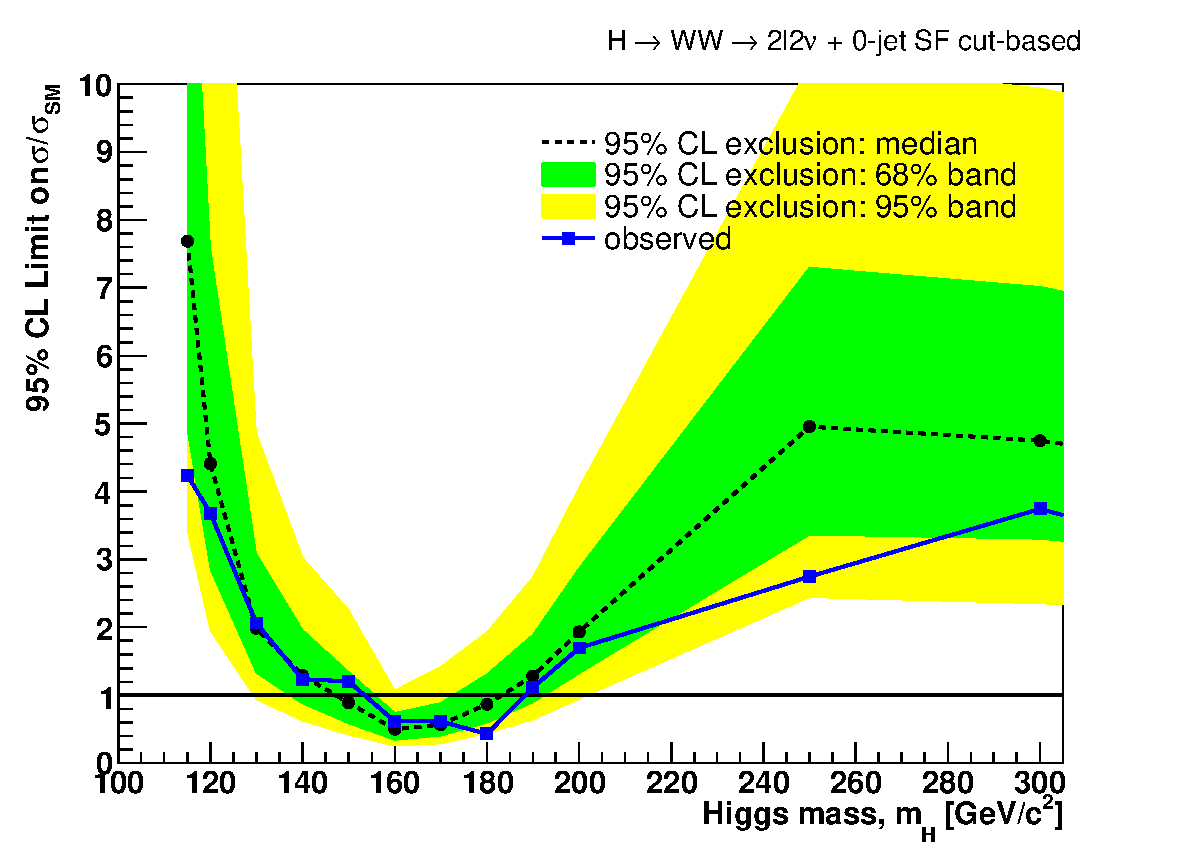
\includegraphics[width=0.48\textwidth]{lp_figures/limits_0j_sf_cut.pdf}}
\subfigure[]{
\centering
\label{subfig:lp_0j_of_cut}
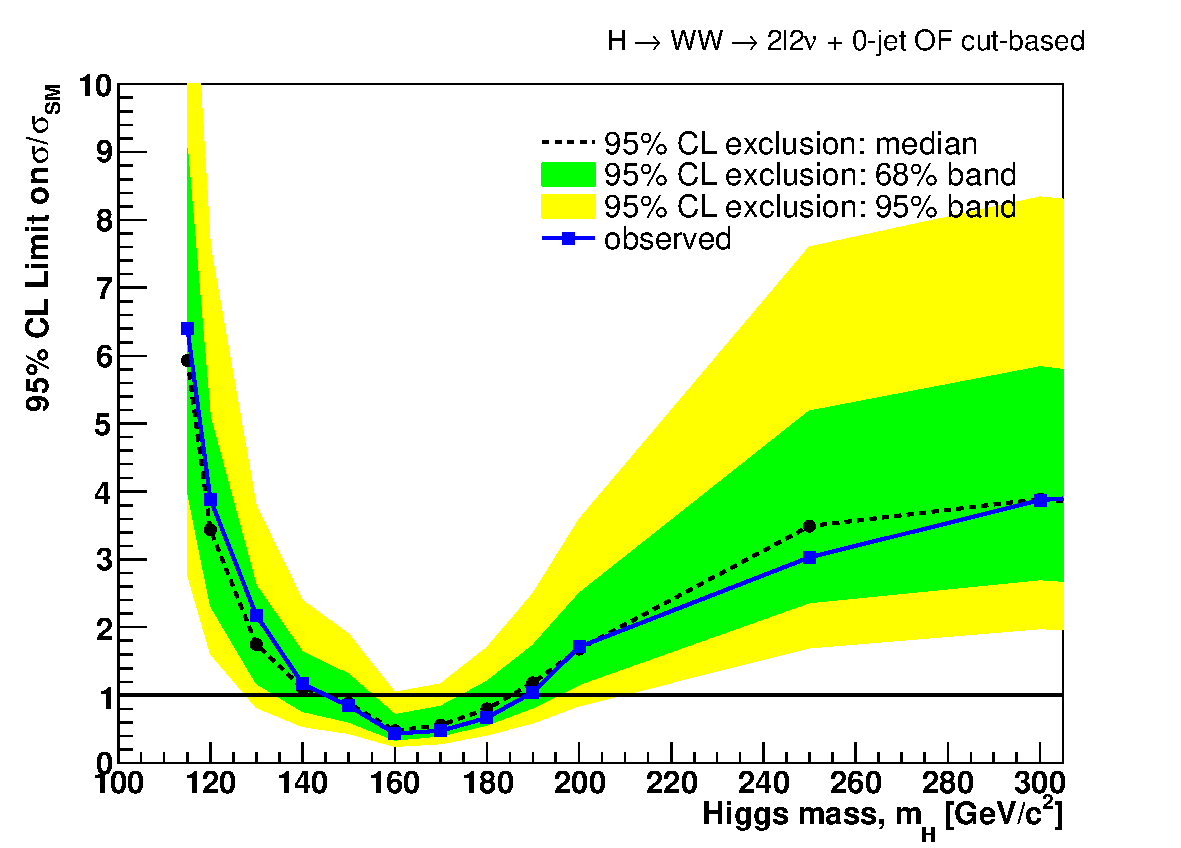
\includegraphics[width=0.48\textwidth]{lp_figures/limits_0j_of_cut.pdf}}
\subfigure[]{
\centering
\label{subfig:eps_0j_sf_cut}
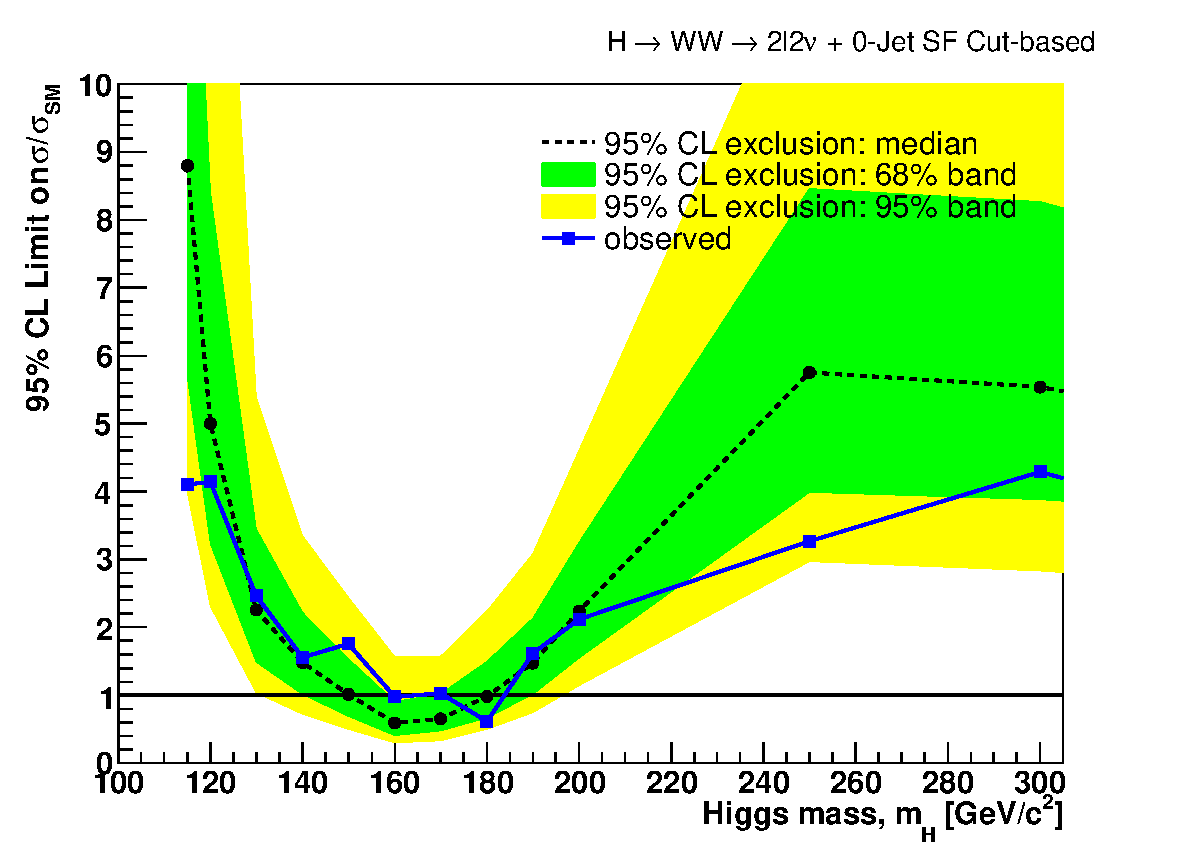
\includegraphics[width=0.48\textwidth]{lp_figures/limits_0j_sf_cut_ana_v6_1500pb_LP_EPS.pdf}}
\subfigure[]{
\centering
\label{subfig:eps_0j_of_cut}
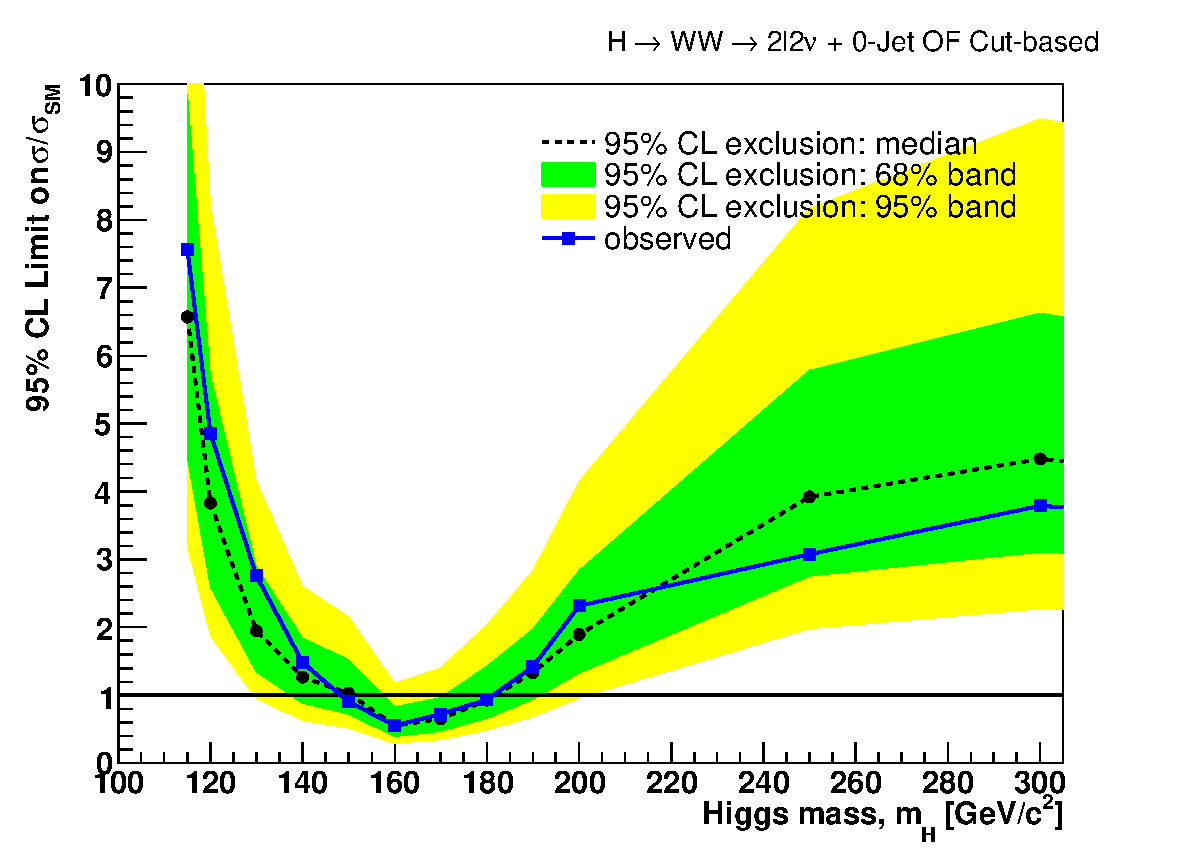
\includegraphics[width=0.48\textwidth]{lp_figures/limits_0j_of_cut_ana_v6_1500pb_LP_EPS.pdf}}
\subfigure[]{
\centering
\label{subfig:post_0j_sf_cut}
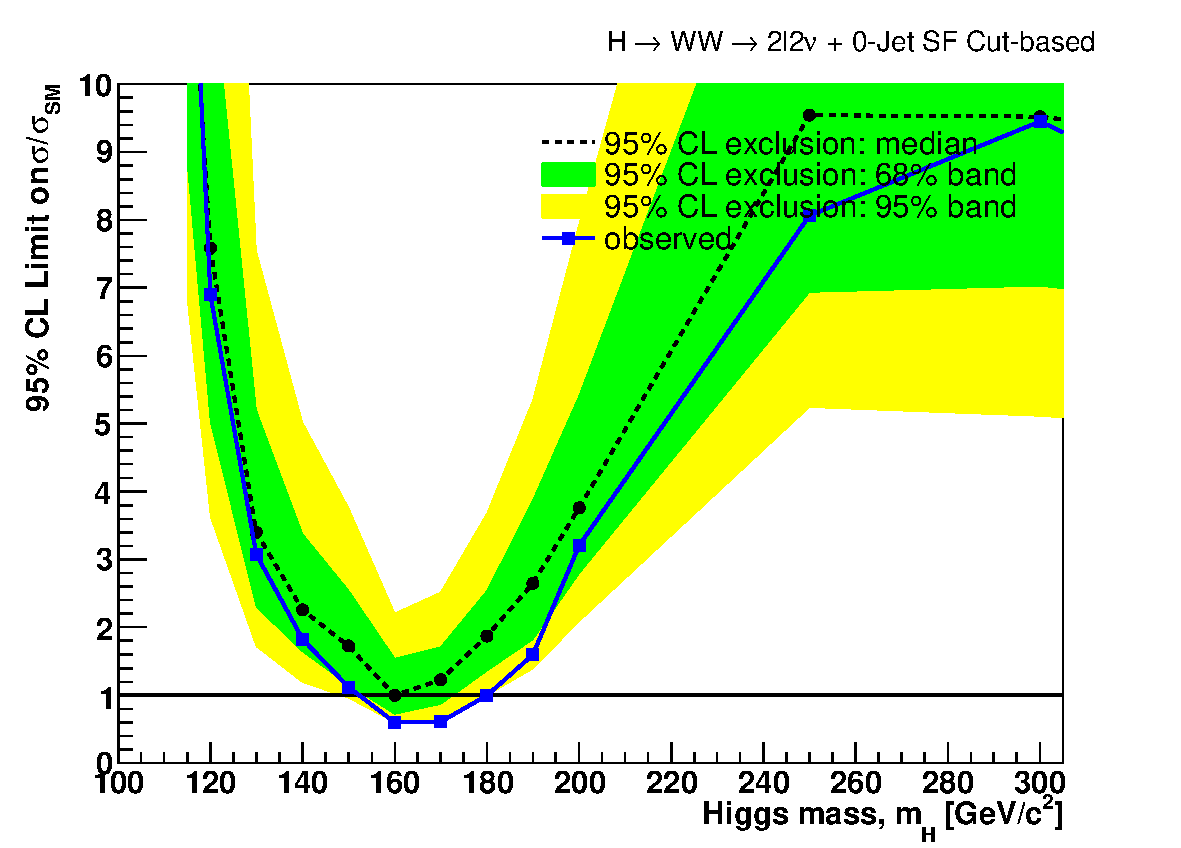
\includegraphics[width=0.48\textwidth]{lp_figures/limits_0j_sf_cut_ana_v6_1500pb_LP_POSTEPS.pdf}}
\subfigure[]{
\centering
\label{subfig:post_0j_of_cut}
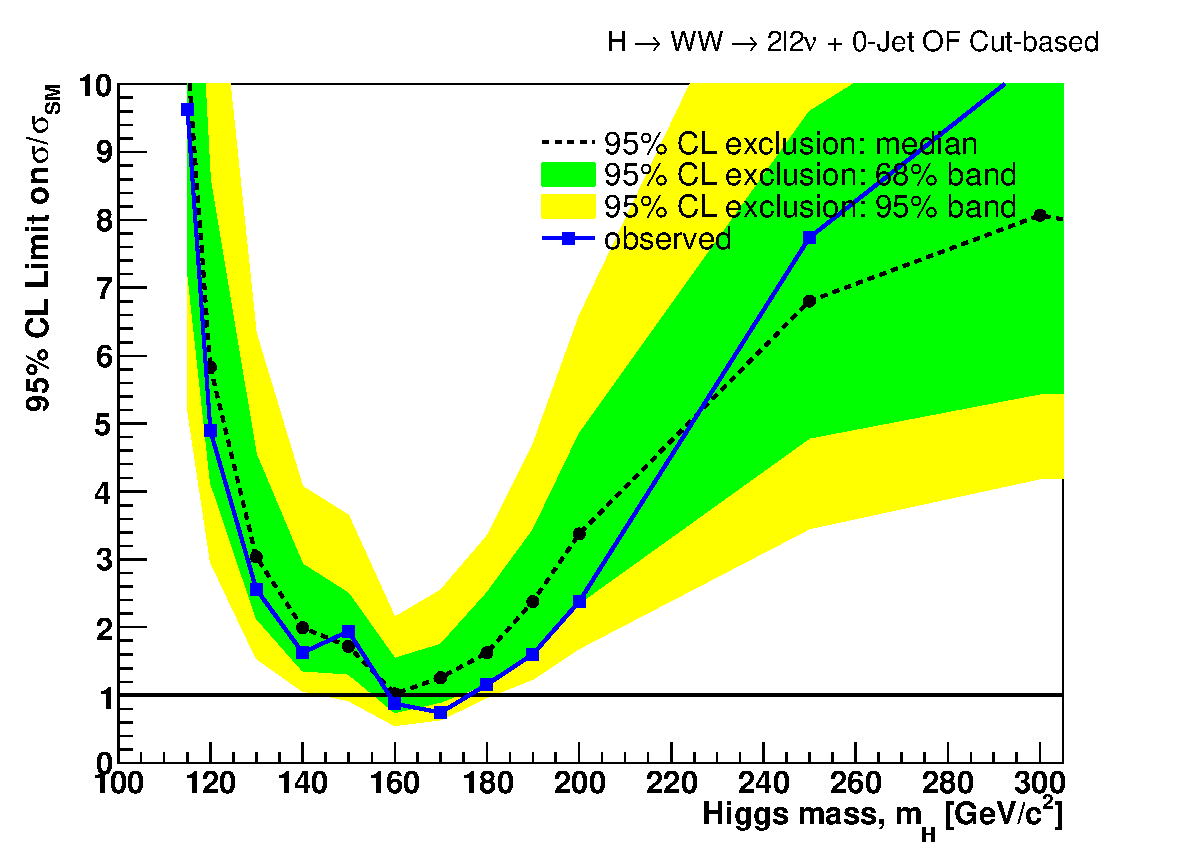
\includegraphics[width=0.48\textwidth]{lp_figures/limits_0j_of_cut_ana_v6_1500pb_LP_POSTEPS.pdf}}
\caption{Cut-based analysis upper limits at 95\% C.L. using LP, EPS and post-EPS datasets for 0-jet events.
\subref{subfig:lp_0j_sf_cut}: LP same-flavor; \subref{subfig:lp_0j_of_cut}: LP opposite-flavor;
\subref{subfig:eps_0j_sf_cut}: EPS same-flavor; \subref{subfig:eps_0j_of_cut}: EPS opposite-flavor;
\subref{subfig:post_0j_sf_cut}: post-EPS same-flavor; \subref{subfig:post_0j_of_cut}: post-EPS opposite-flavor;
}
\label{fig:limits_0j_cut}
\end{figure}

\clearpage
\subsubsection{Zero-Jet MVA-Based}
\begin{figure}[!htbp]
\centering
\subfigure[]{
\centering
\label{subfig:lp_0j_sf_shape}
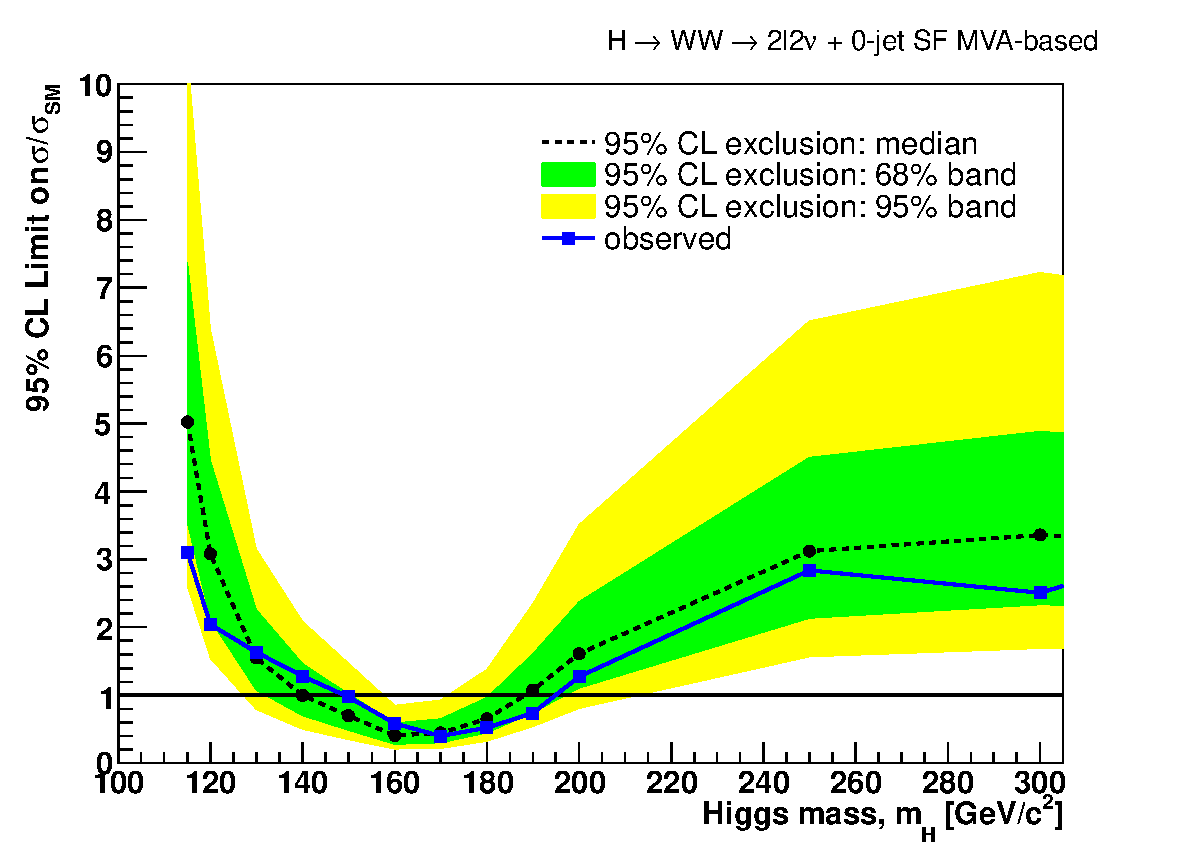
\includegraphics[width=0.48\textwidth]{lp_figures/limits_0j_sf_shape.pdf}}
\subfigure[]{
\centering
\label{subfig:lp_0j_of_shape}
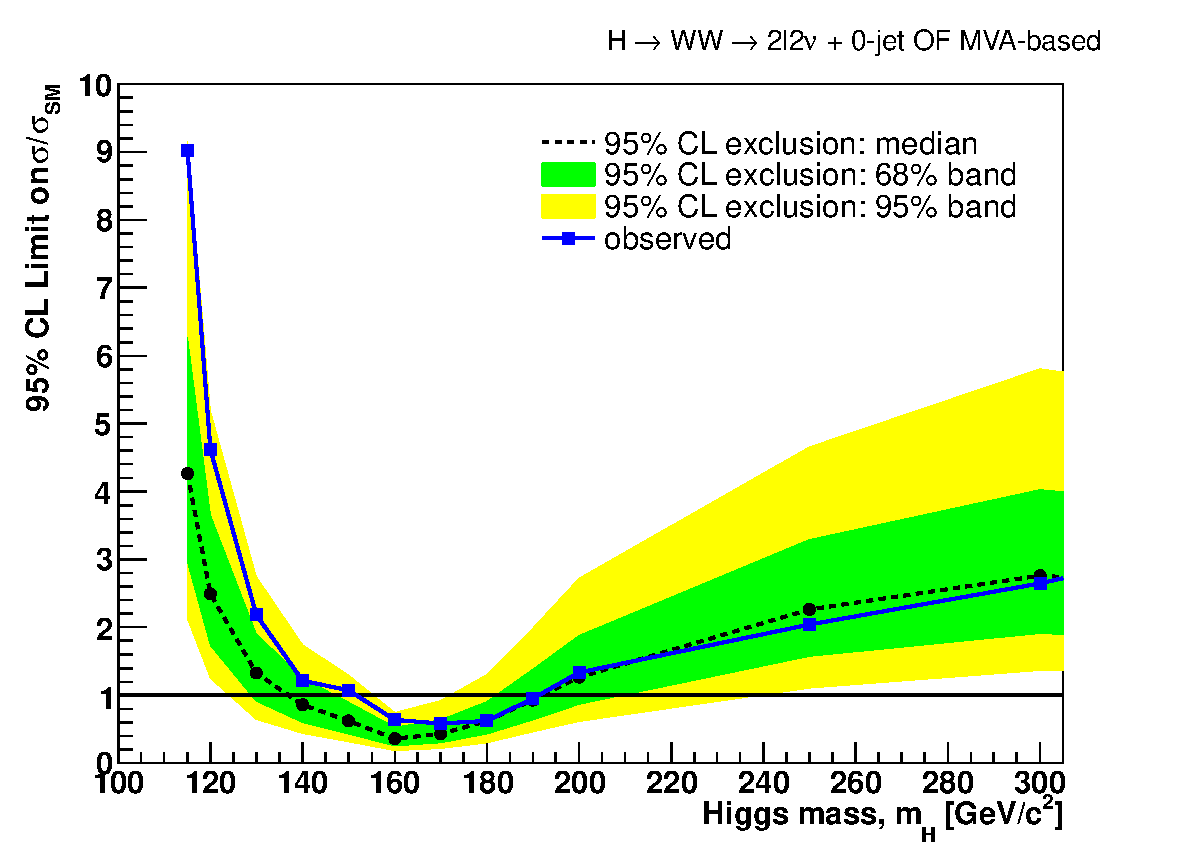
\includegraphics[width=0.48\textwidth]{lp_figures/limits_0j_of_shape.pdf}}
\subfigure[]{
\centering
\label{subfig:eps_0j_sf_shape}
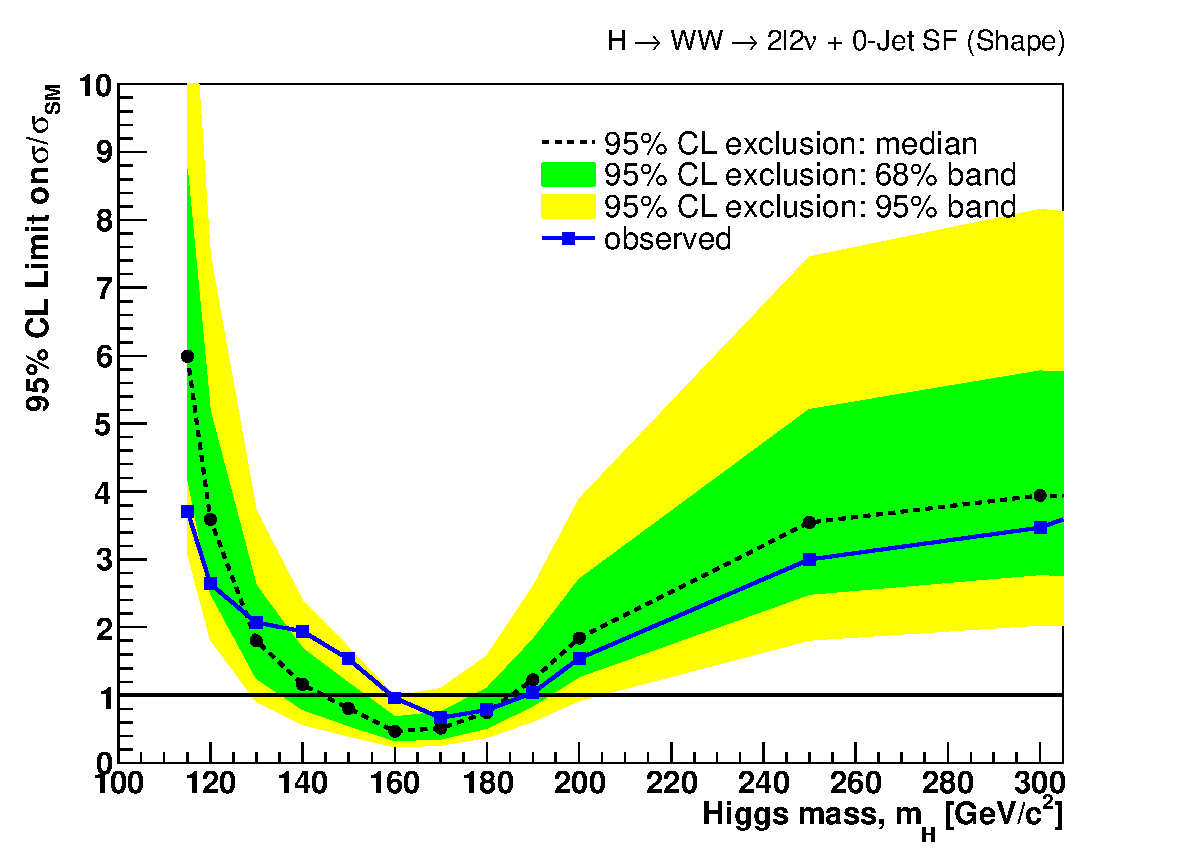
\includegraphics[width=0.48\textwidth]{lp_figures/limits_0j_sf_shape_ana_v6_1500pb_LP_EPS.pdf}}
\subfigure[]{
\centering
\label{subfig:eps_0j_of_shape}
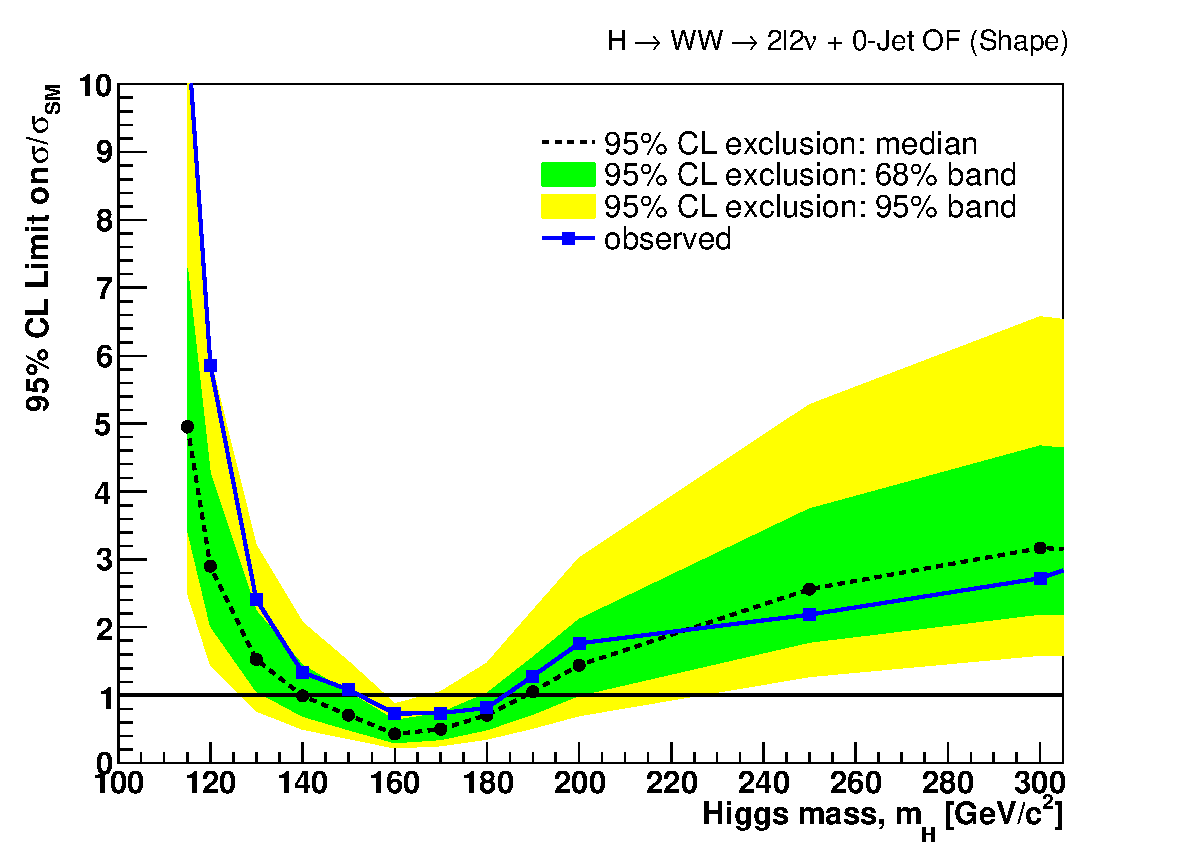
\includegraphics[width=0.48\textwidth]{lp_figures/limits_0j_of_shape_ana_v6_1500pb_LP_EPS.pdf}}
\subfigure[]{
\centering
\label{subfig:post_0j_sf_shape}
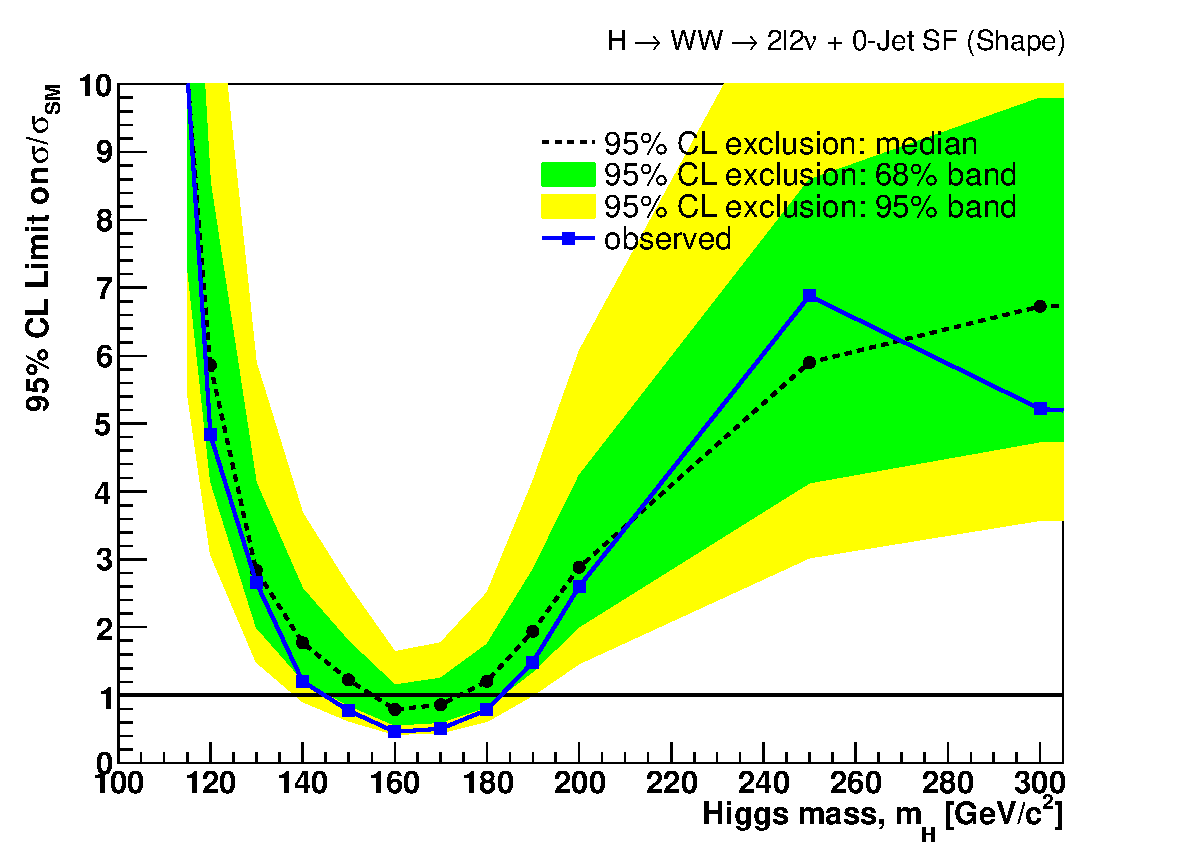
\includegraphics[width=0.48\textwidth]{lp_figures/limits_0j_sf_shape_ana_v6_1500pb_LP_POSTEPS.pdf}}
\subfigure[]{
\centering
\label{subfig:post_0j_of_shape}
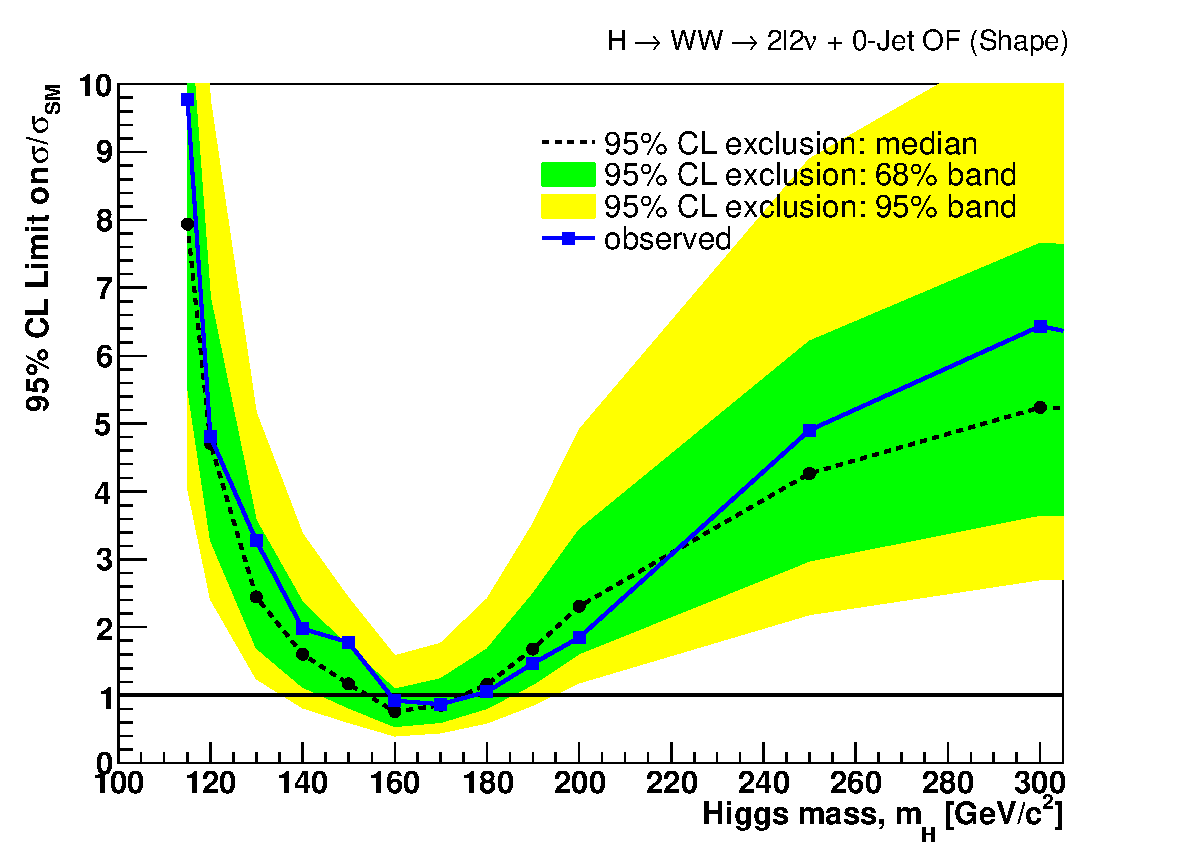
\includegraphics[width=0.48\textwidth]{lp_figures/limits_0j_of_shape_ana_v6_1500pb_LP_POSTEPS.pdf}}
\caption{Multivariate-based analysis upper limits at 95\% C.L. using LP, EPS and post-EPS datasets for 0-jet events.
\subref{subfig:lp_0j_sf_shape}: LP same-flavor; \subref{subfig:lp_0j_of_shape}: LP opposite-flavor;
\subref{subfig:eps_0j_sf_shape}: EPS same-flavor; \subref{subfig:eps_0j_of_shape}: EPS opposite-flavor;
\subref{subfig:post_0j_sf_shape}: post-EPS same-flavor; \subref{subfig:post_0j_of_shape}: post-EPS opposite-flavor;
}
\label{fig:limits_0j_shape}
\end{figure}

\clearpage
\subsubsection{One-Jet Cut-Based}
\begin{figure}[!htbp]
\centering
\subfigure[]{
\centering
\label{subfig:lp_1j_sf_cut}
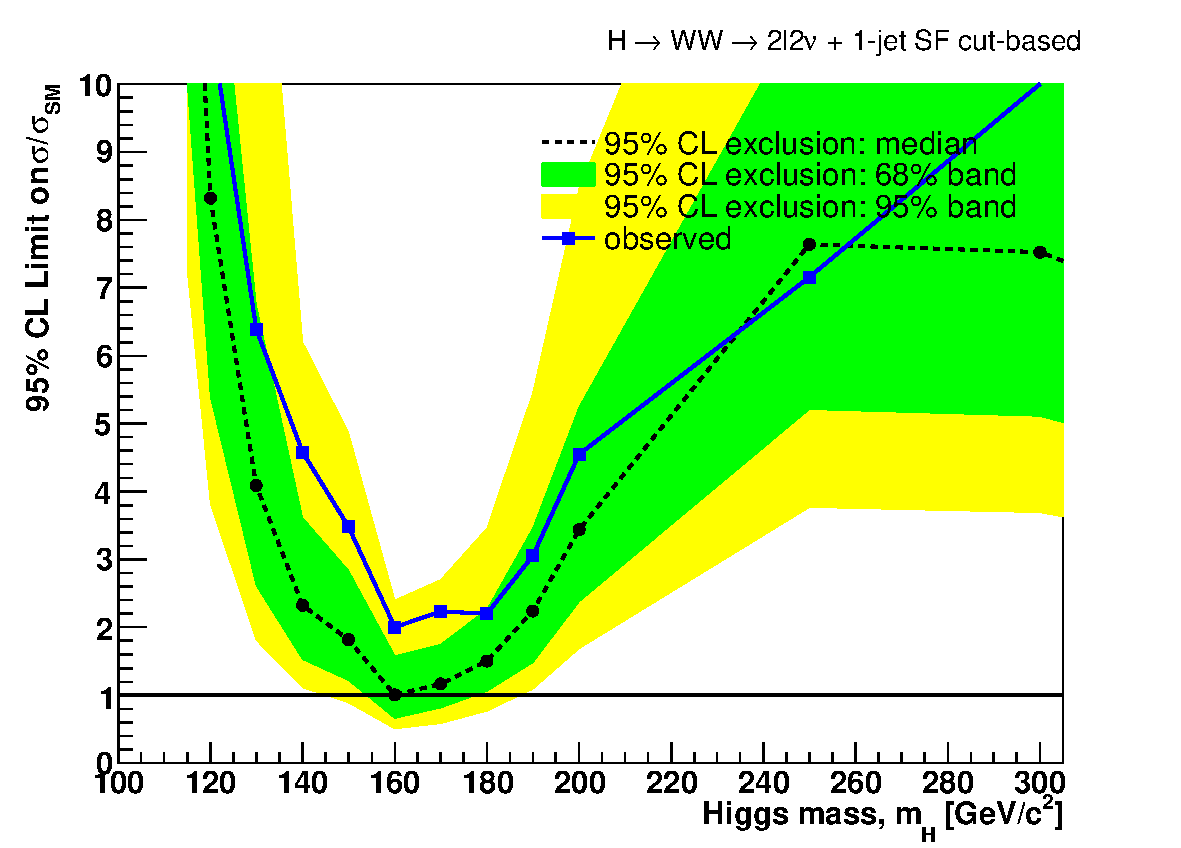
\includegraphics[width=0.48\textwidth]{lp_figures/limits_1j_sf_cut.pdf}}
\subfigure[]{
\centering
\label{subfig:lp_1j_of_cut}
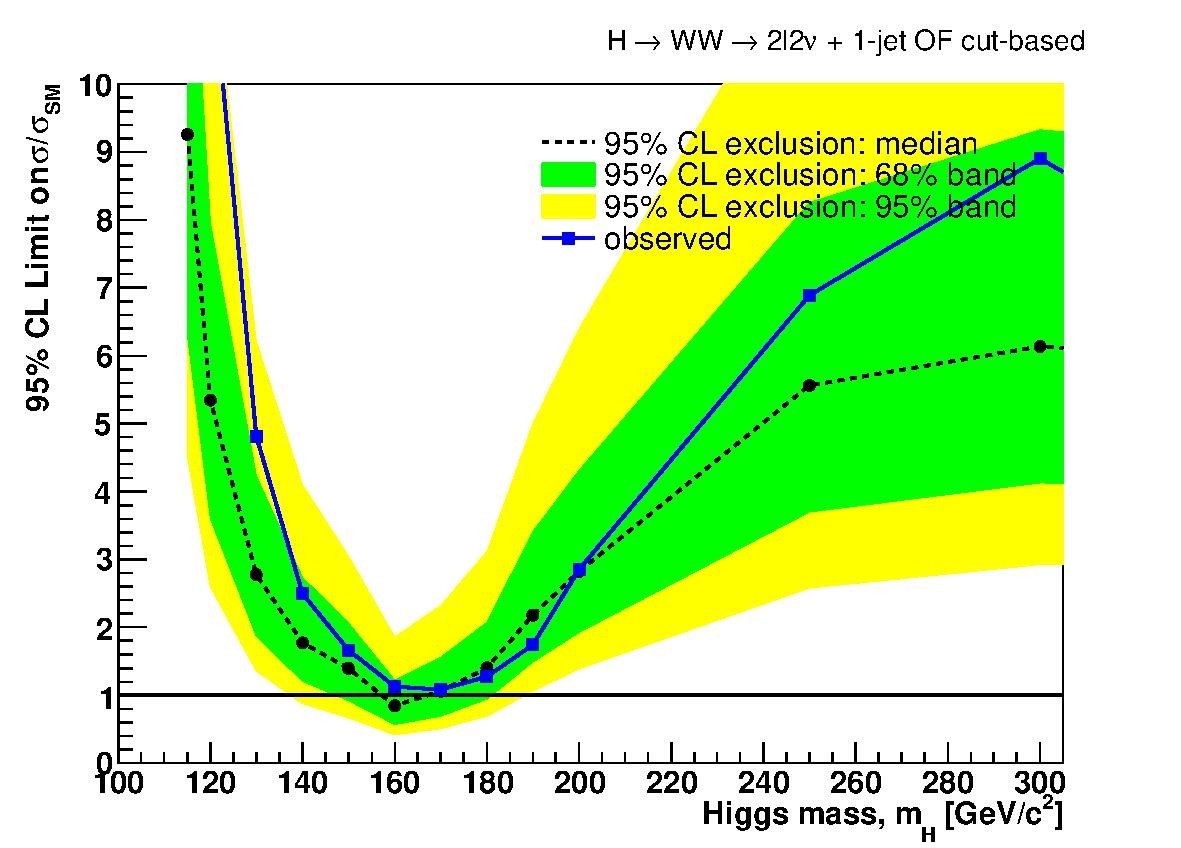
\includegraphics[width=0.48\textwidth]{lp_figures/limits_1j_of_cut.pdf}}
\subfigure[]{
\centering
\label{subfig:eps_1j_sf_cut}
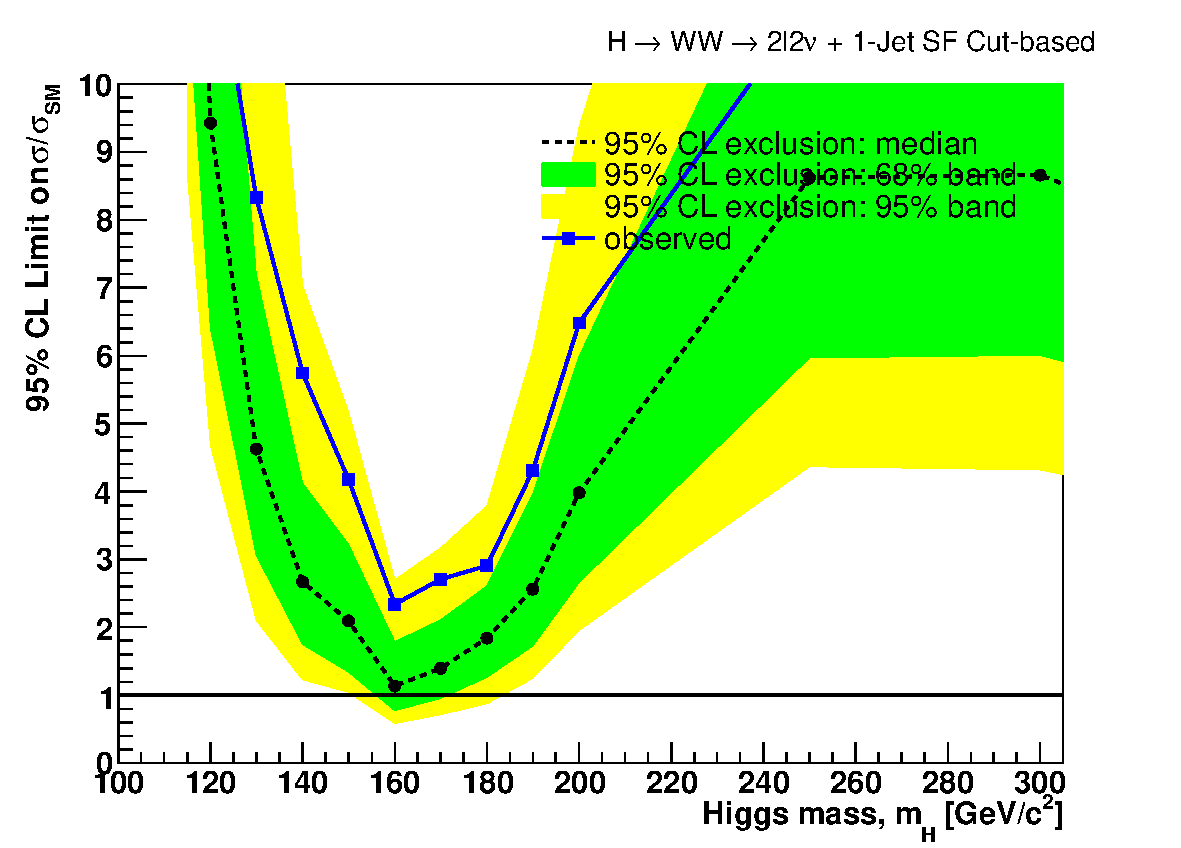
\includegraphics[width=0.48\textwidth]{lp_figures/limits_1j_sf_cut_ana_v6_1500pb_LP_EPS.pdf}}
\subfigure[]{
\centering
\label{subfig:eps_1j_of_cut}
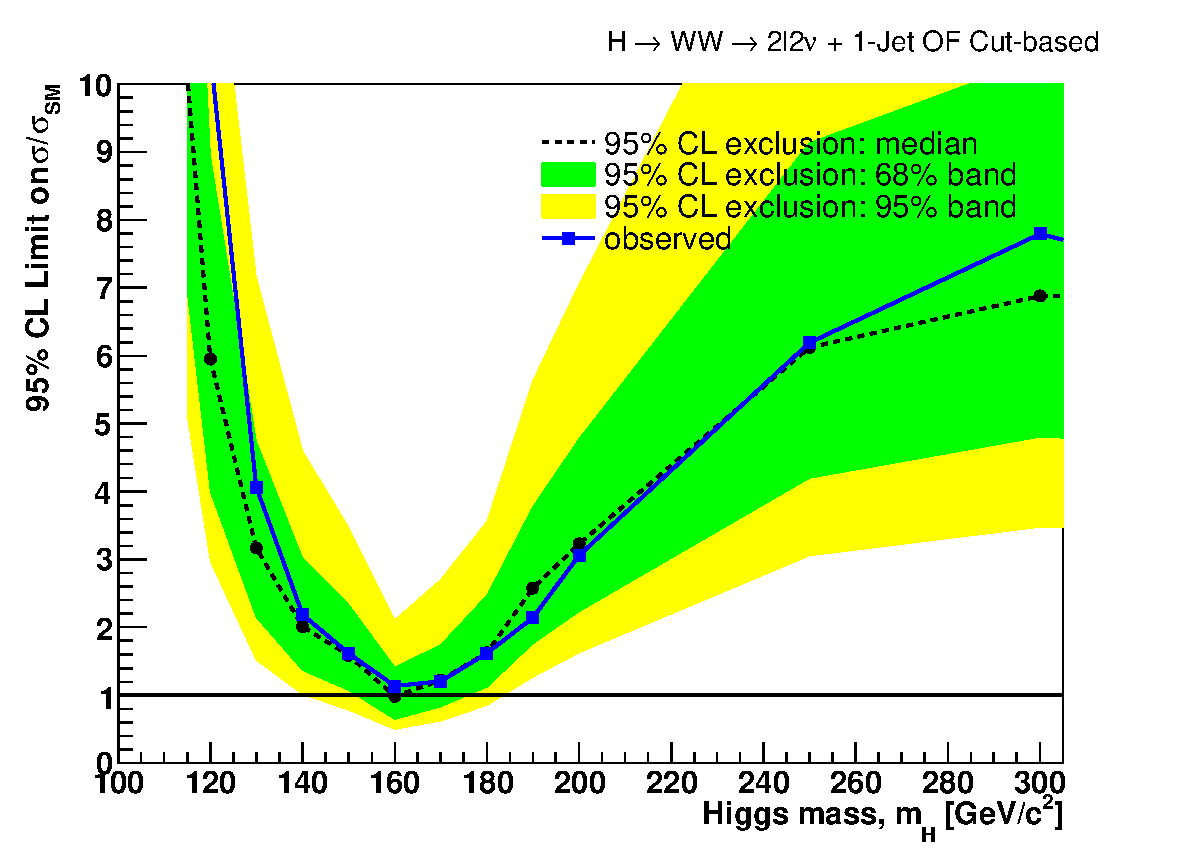
\includegraphics[width=0.48\textwidth]{lp_figures/limits_1j_of_cut_ana_v6_1500pb_LP_EPS.pdf}}
\subfigure[]{
\centering
\label{subfig:post_1j_sf_cut}
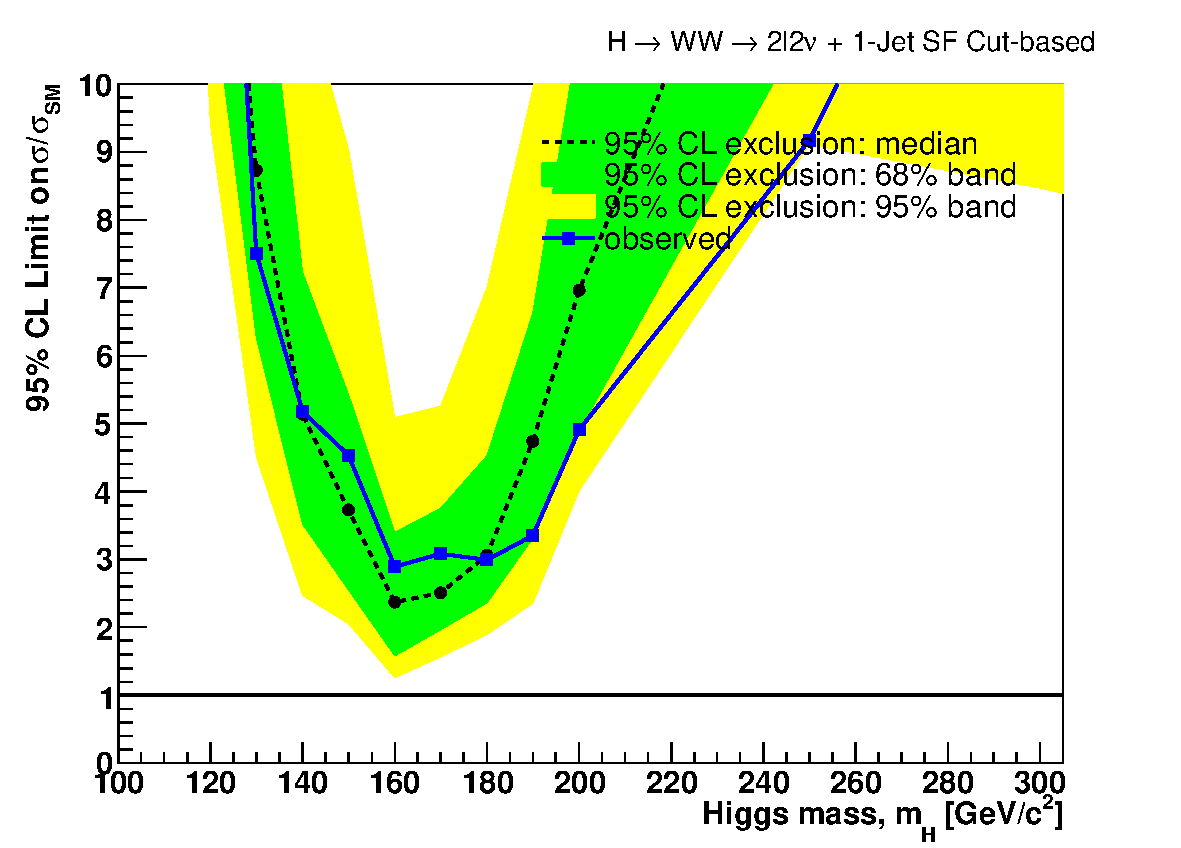
\includegraphics[width=0.48\textwidth]{lp_figures/limits_1j_sf_cut_ana_v6_1500pb_LP_POSTEPS.pdf}}
\subfigure[]{
\centering
\label{subfig:post_1j_of_cut}
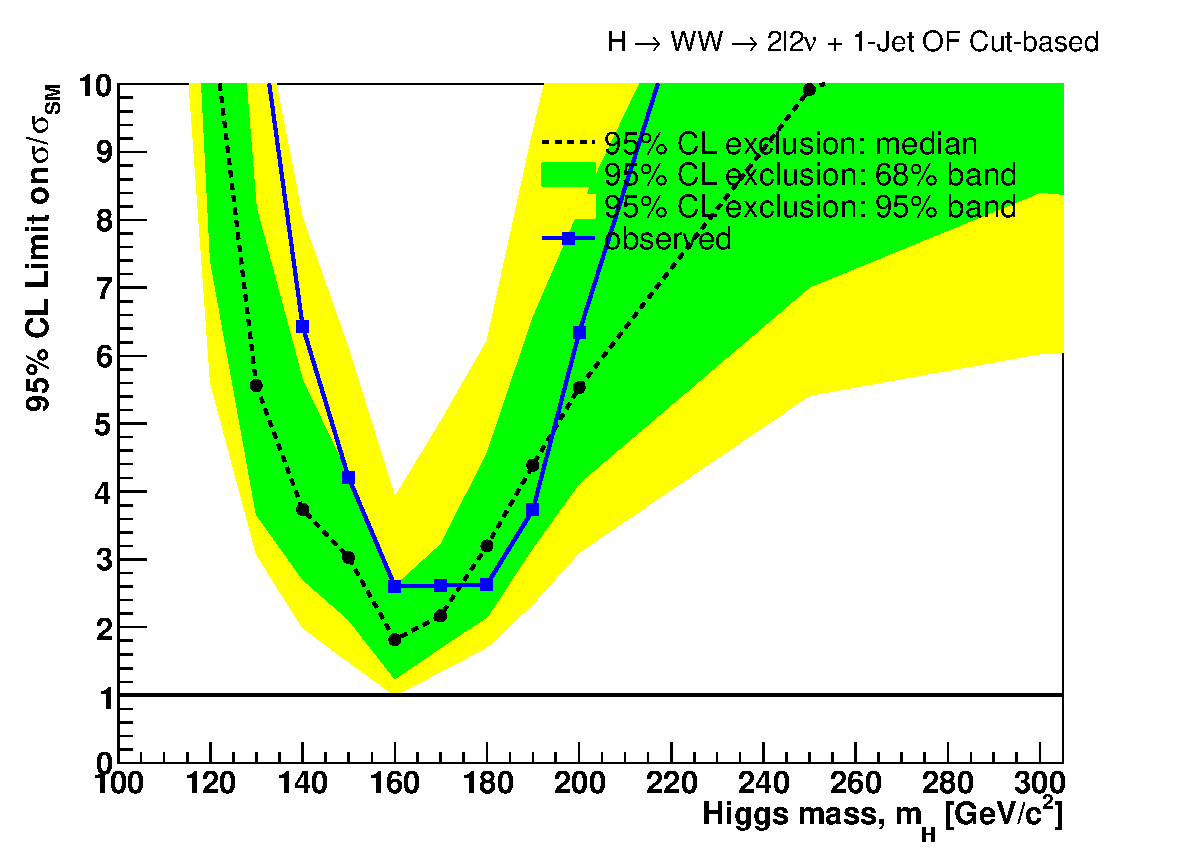
\includegraphics[width=0.48\textwidth]{lp_figures/limits_1j_of_cut_ana_v6_1500pb_LP_POSTEPS.pdf}}
\caption{Cut-based analysis upper limits at 95\% C.L. using LP, EPS and post-EPS datasets for 1-jet events.
\subref{subfig:lp_1j_sf_cut}: LP same-flavor; \subref{subfig:lp_1j_of_cut}: LP opposite-flavor;
\subref{subfig:eps_1j_sf_cut}: EPS same-flavor; \subref{subfig:eps_1j_of_cut}: EPS opposite-flavor;
\subref{subfig:post_1j_sf_cut}: post-EPS same-flavor; \subref{subfig:post_1j_of_cut}: post-EPS opposite-flavor;
}
\label{fig:limits_1j_cut}
\end{figure}

\clearpage
\subsubsection{One-Jet MVA-Based}
\begin{figure}[!htbp]
\centering
\subfigure[]{
\centering
\label{subfig:lp_1j_sf_shape}
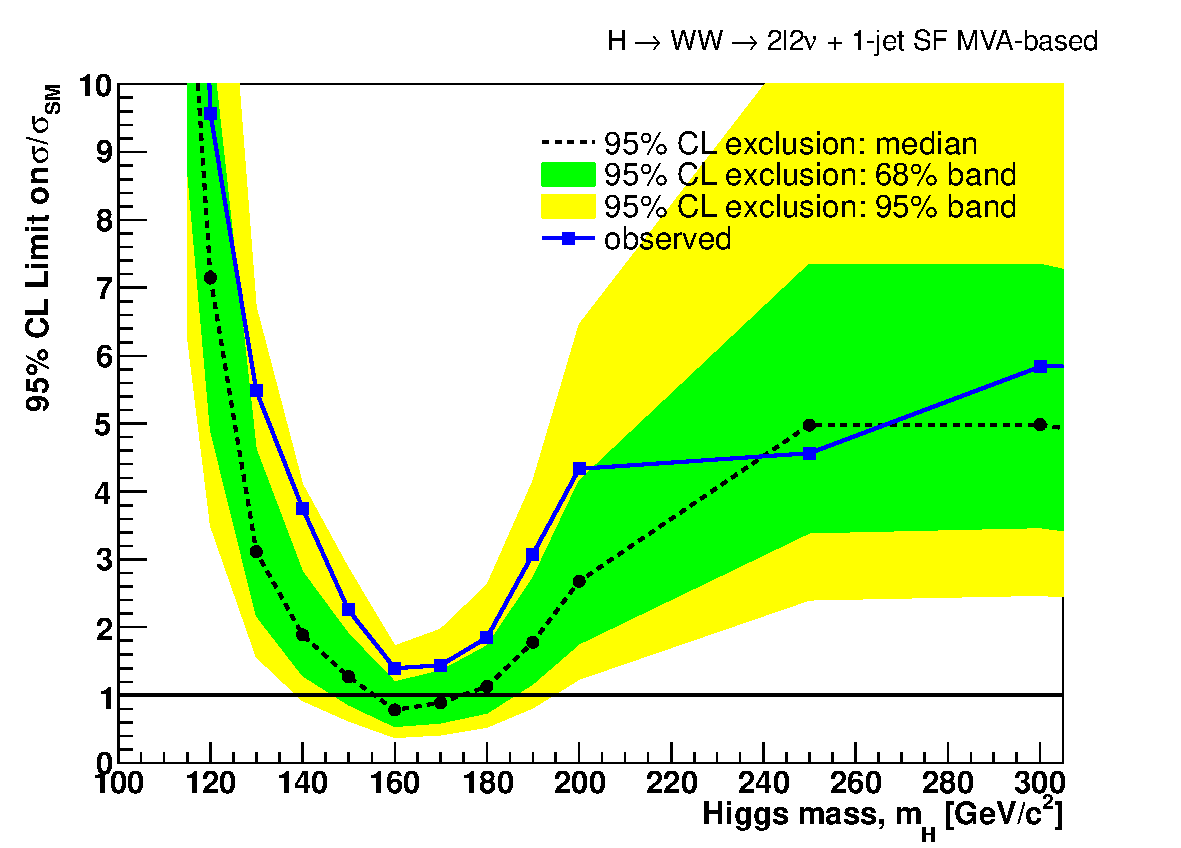
\includegraphics[width=0.48\textwidth]{lp_figures/limits_1j_sf_shape.pdf}}
\subfigure[]{
\centering
\label{subfig:lp_1j_of_shape}
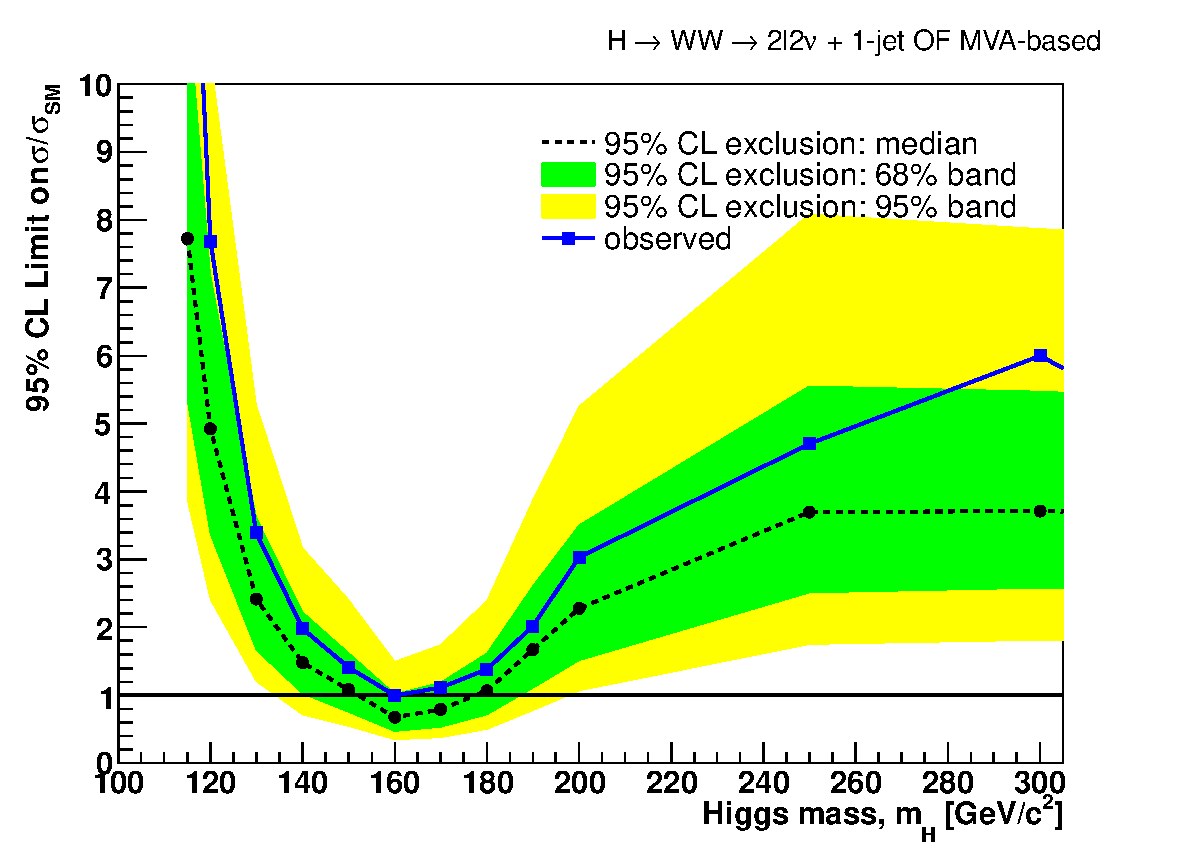
\includegraphics[width=0.48\textwidth]{lp_figures/limits_1j_of_shape.pdf}}
\subfigure[]{
\centering
\label{subfig:eps_1j_sf_shape}
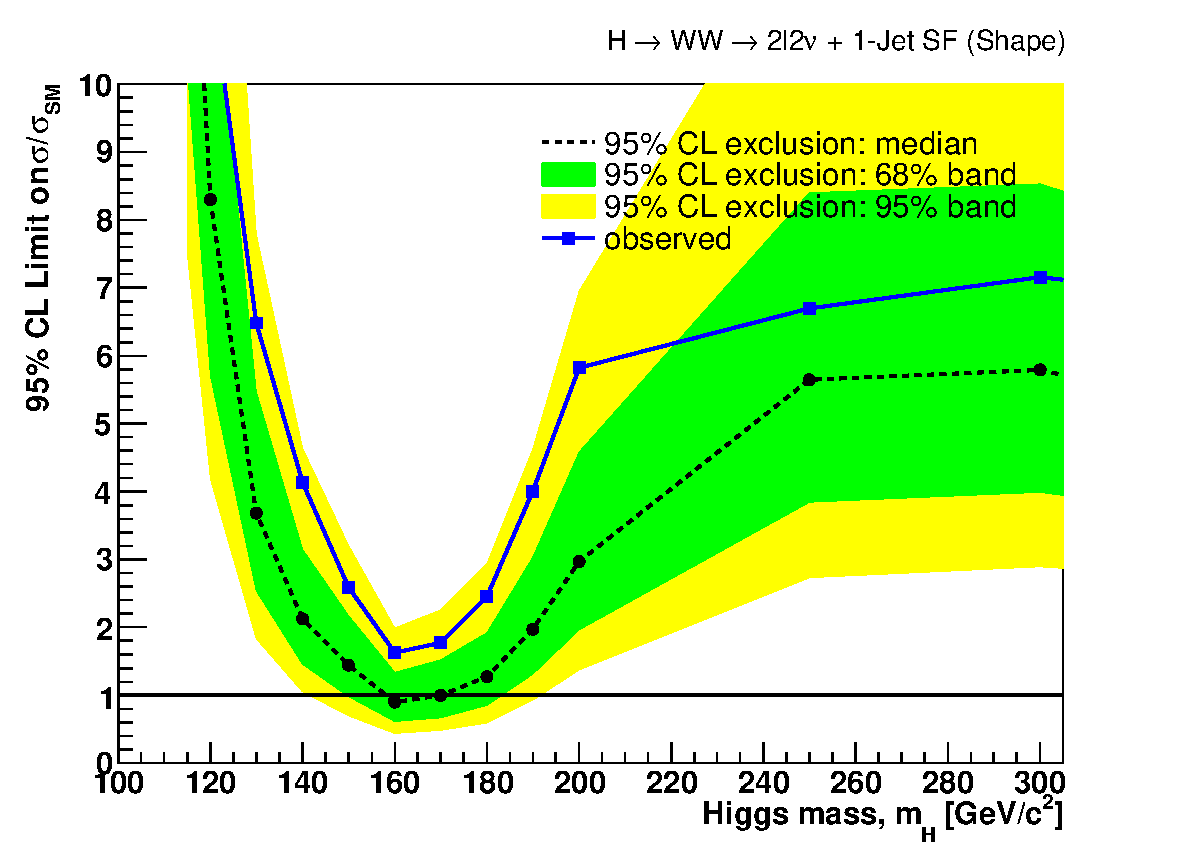
\includegraphics[width=0.48\textwidth]{lp_figures/limits_1j_sf_shape_ana_v6_1500pb_LP_EPS.pdf}}
\subfigure[]{
\centering
\label{subfig:eps_1j_of_shape}
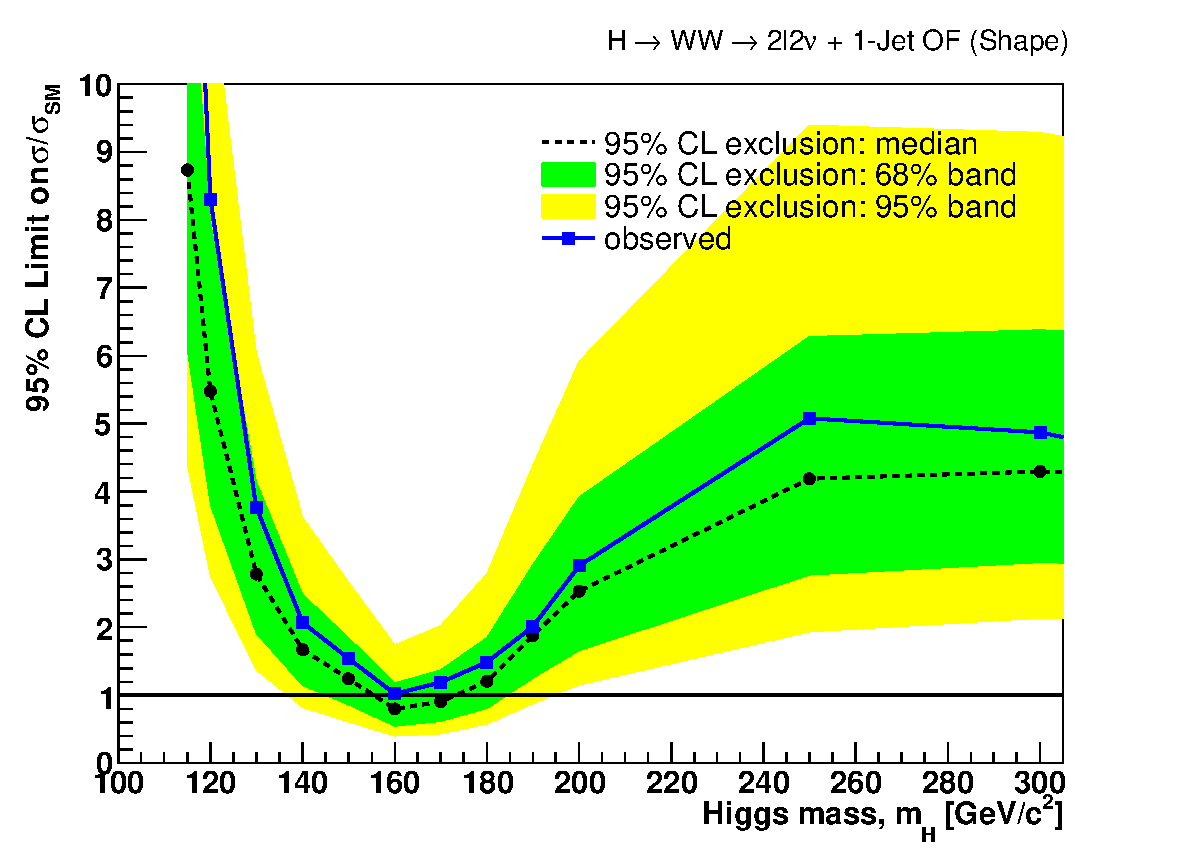
\includegraphics[width=0.48\textwidth]{lp_figures/limits_1j_of_shape_ana_v6_1500pb_LP_EPS.pdf}}
\subfigure[]{
\centering
\label{subfig:post_1j_sf_shape}
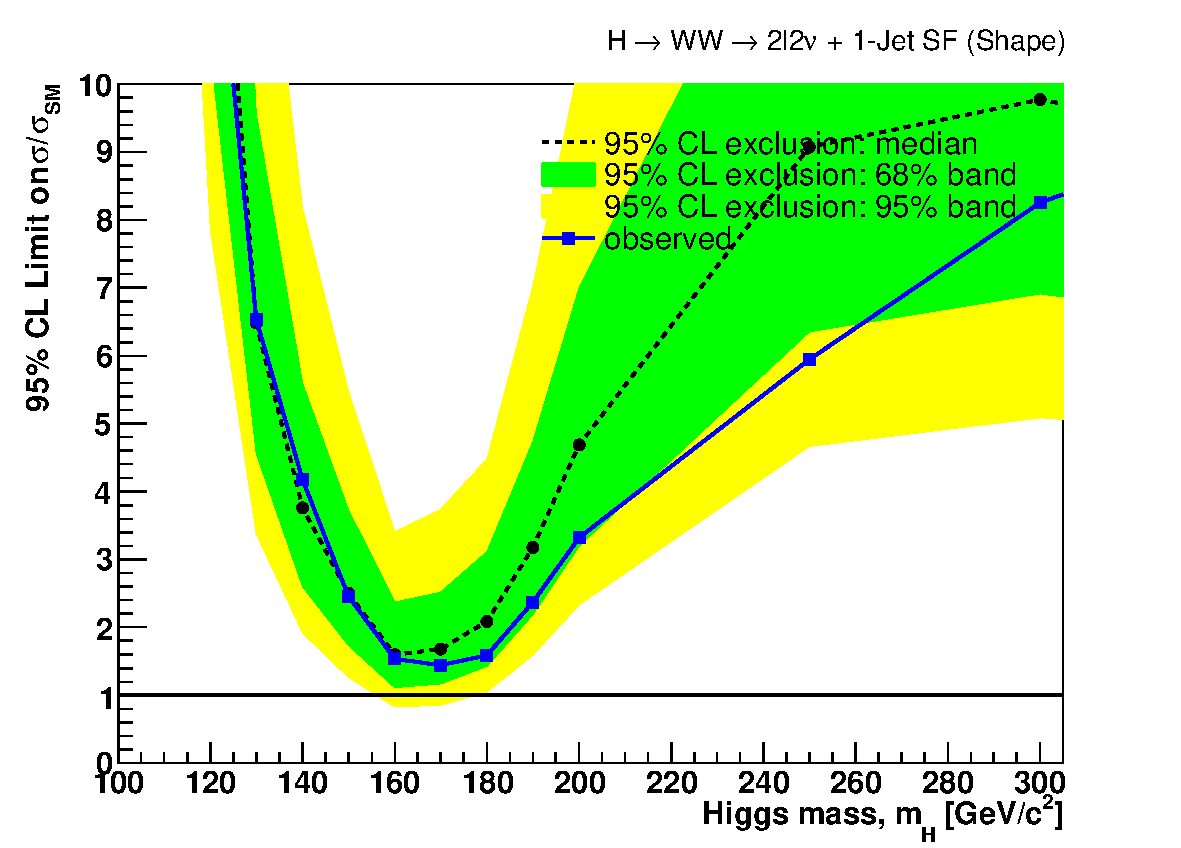
\includegraphics[width=0.48\textwidth]{lp_figures/limits_1j_sf_shape_ana_v6_1500pb_LP_POSTEPS.pdf}}
\subfigure[]{
\centering
\label{subfig:post_1j_of_shape}
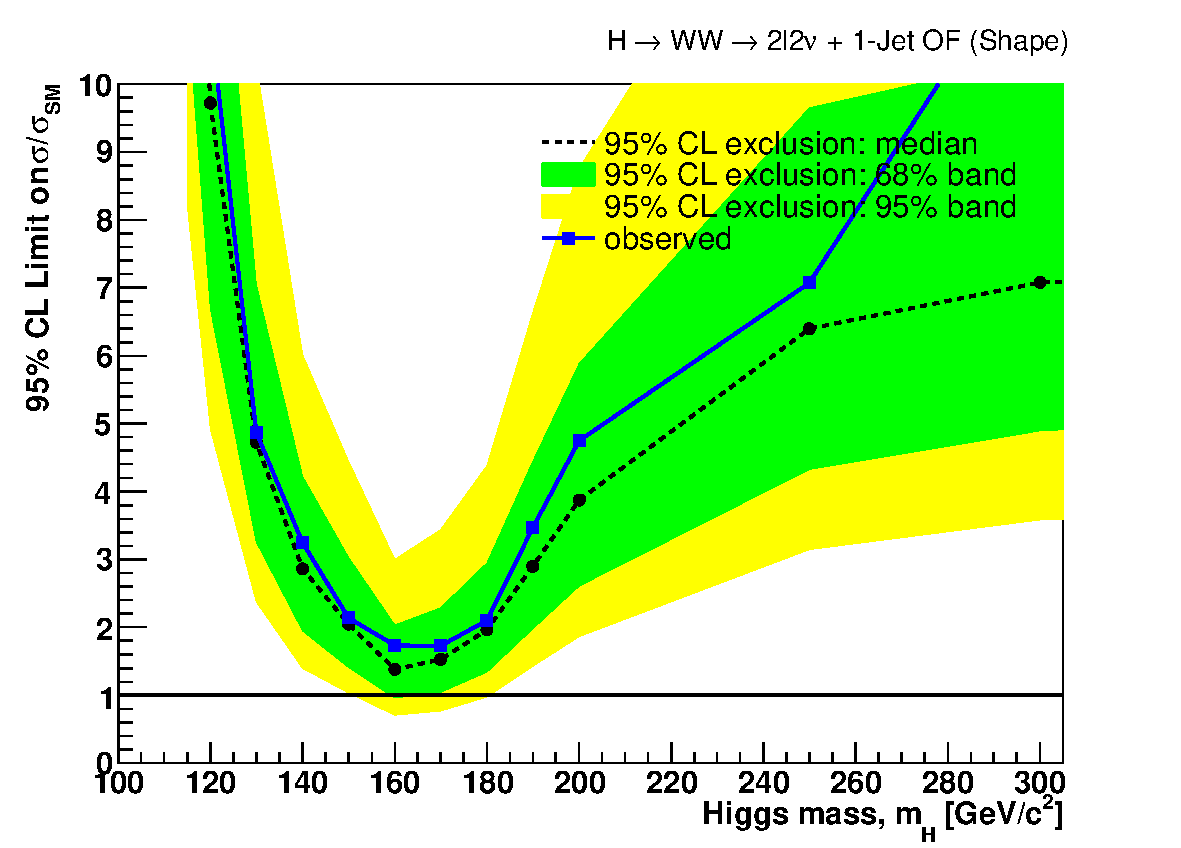
\includegraphics[width=0.48\textwidth]{lp_figures/limits_1j_of_shape_ana_v6_1500pb_LP_POSTEPS.pdf}}
\caption{Multivariate-based analysis upper limits at 95\% C.L. using LP, EPS and post-EPS datasets for 1-jet events.
\subref{subfig:lp_1j_sf_shape}: LP same-flavor; \subref{subfig:lp_1j_of_shape}: LP opposite-flavor;
\subref{subfig:eps_1j_sf_shape}: EPS same-flavor; \subref{subfig:eps_1j_of_shape}: EPS opposite-flavor;
\subref{subfig:post_1j_sf_shape}: post-EPS same-flavor; \subref{subfig:post_1j_of_shape}: post-EPS opposite-flavor;
}
\label{fig:limits_1j_shape}
\end{figure}


%%%%%%%%%%%%%%%%%%%%%%%%%%%%%%
\clearpage
\subsubsection{Cut-Based with Additional Transverse Mass Requirement}
\begin{figure}[!htbp]
\centering
\subfigure[]{
\centering
\label{subfig:0j_sf}
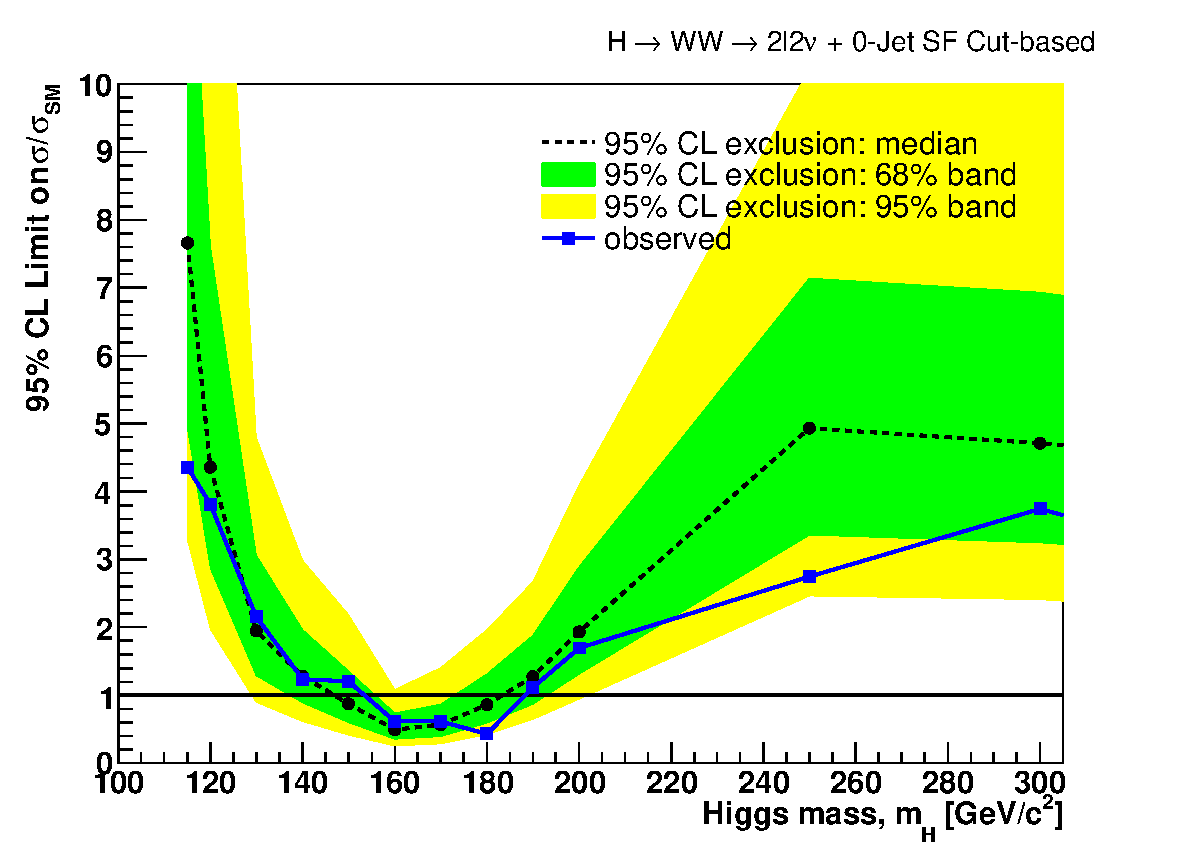
\includegraphics[width=0.48\textwidth]{lp_figures/limits_0j_sf_cut_ana_v6_1500pb_LP_MTCUT80.pdf}}
\subfigure[]{
\centering
\label{subfig:0j_of}
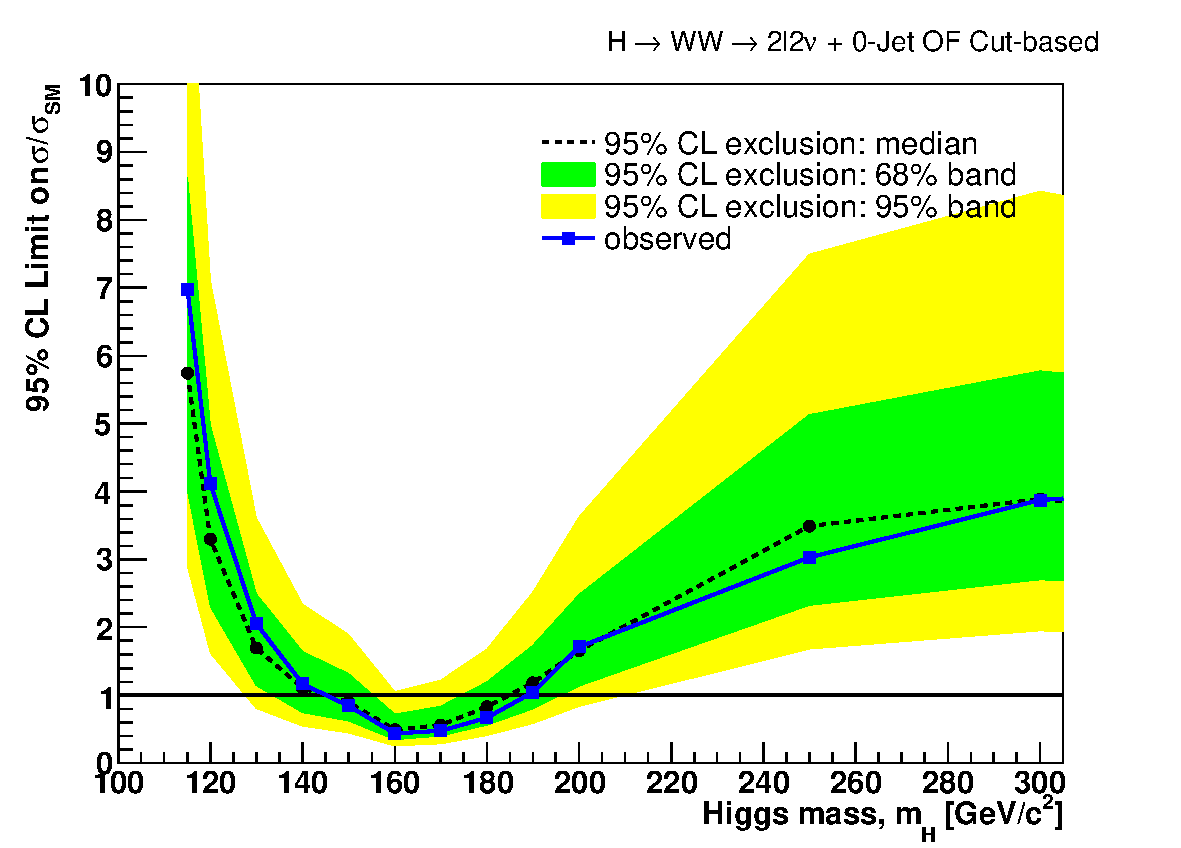
\includegraphics[width=0.48\textwidth]{lp_figures/limits_0j_of_cut_ana_v6_1500pb_LP_MTCUT80.pdf}}
\subfigure[]{
\centering
\label{subfig:1j_sf}
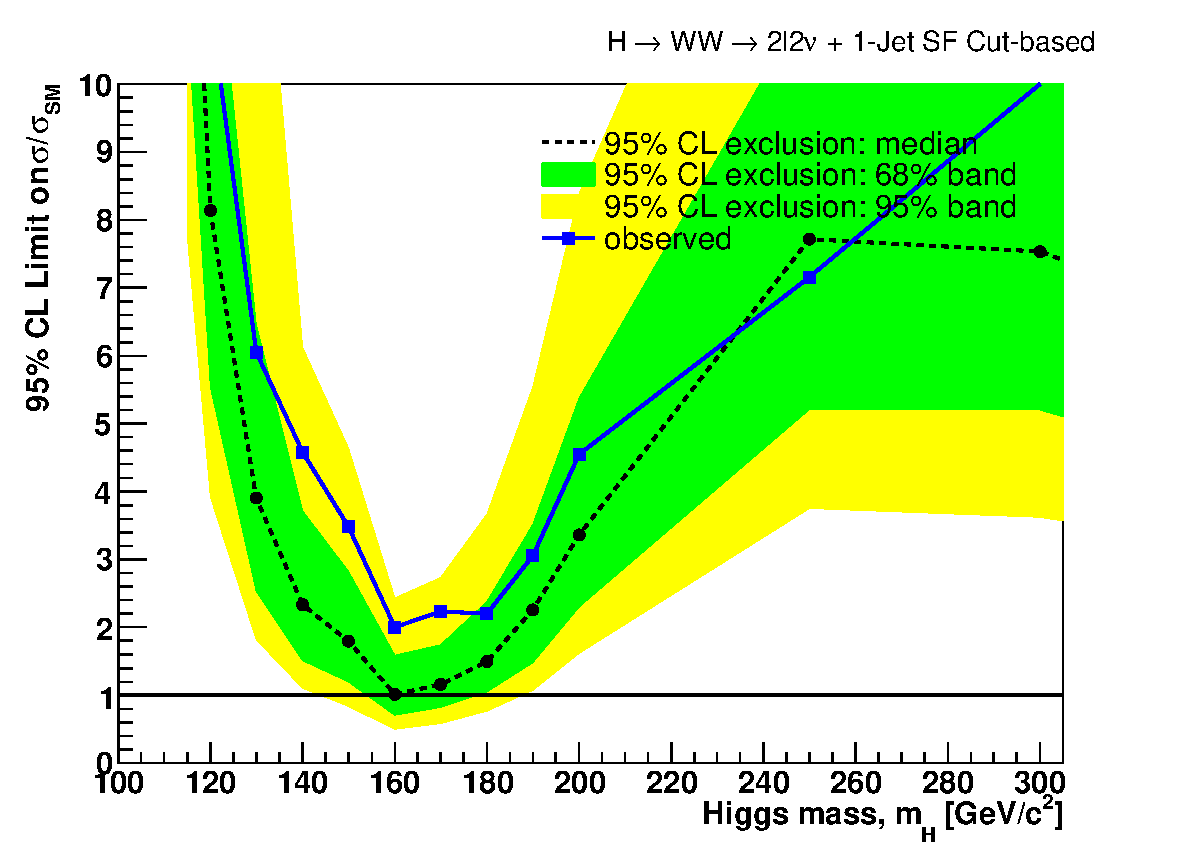
\includegraphics[width=0.48\textwidth]{lp_figures/limits_1j_sf_cut_ana_v6_1500pb_LP_MTCUT80.pdf}}
\subfigure[]{
\centering
\label{subfig:1j_of}
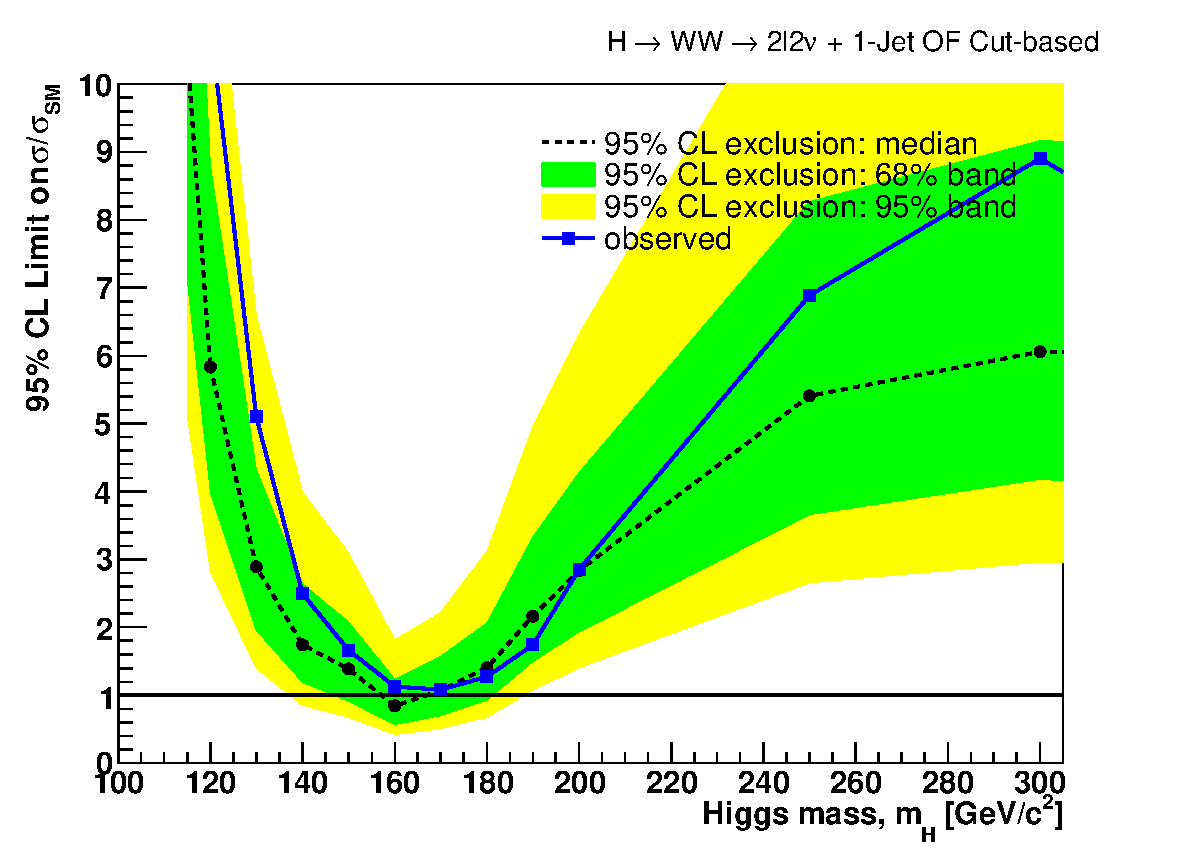
\includegraphics[width=0.48\textwidth]{lp_figures/limits_1j_of_cut_ana_v6_1500pb_LP_MTCUT80.pdf}}
\subfigure[]{
\centering
\label{subfig:2j}
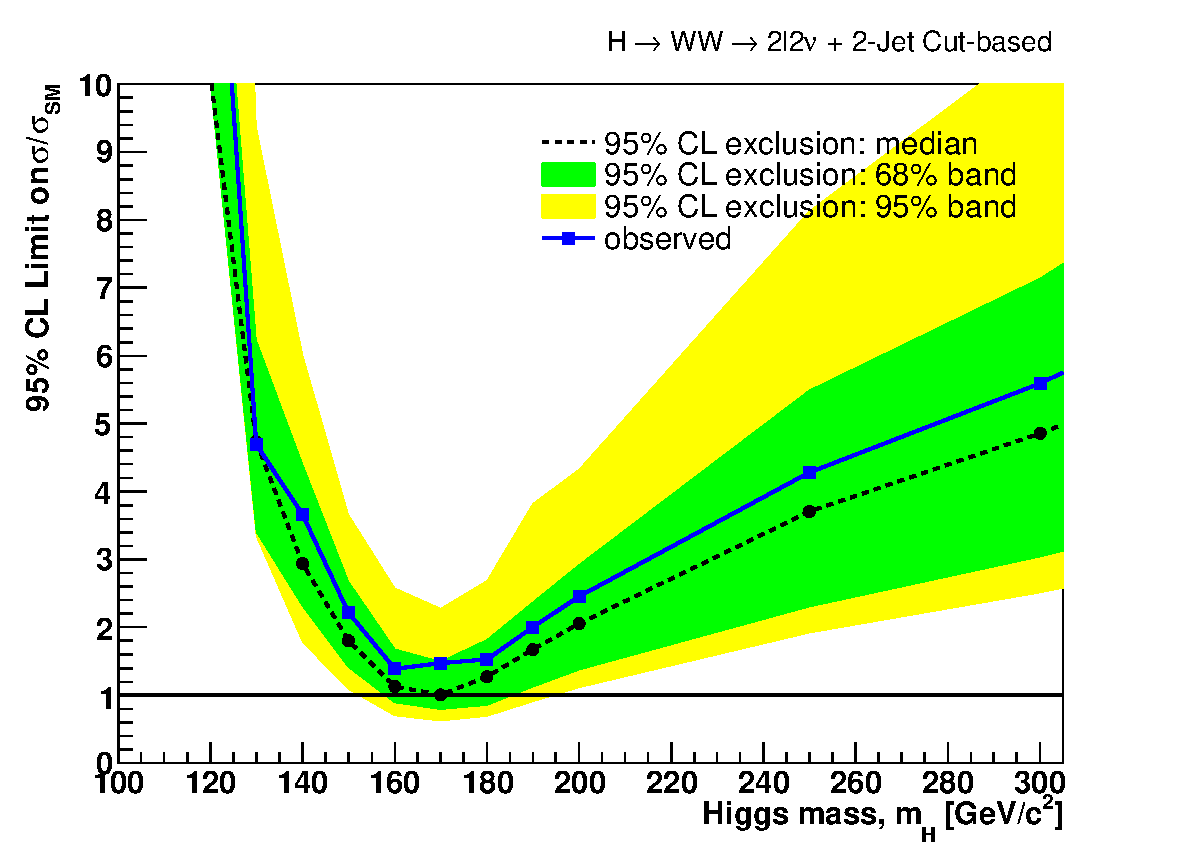
\includegraphics[width=0.48\textwidth]{lp_figures/limits_2j_cut_ana_v6_1500pb_LP_MTCUT80.pdf}}
\subfigure[]{
\centering
\label{subfig:njcomb}
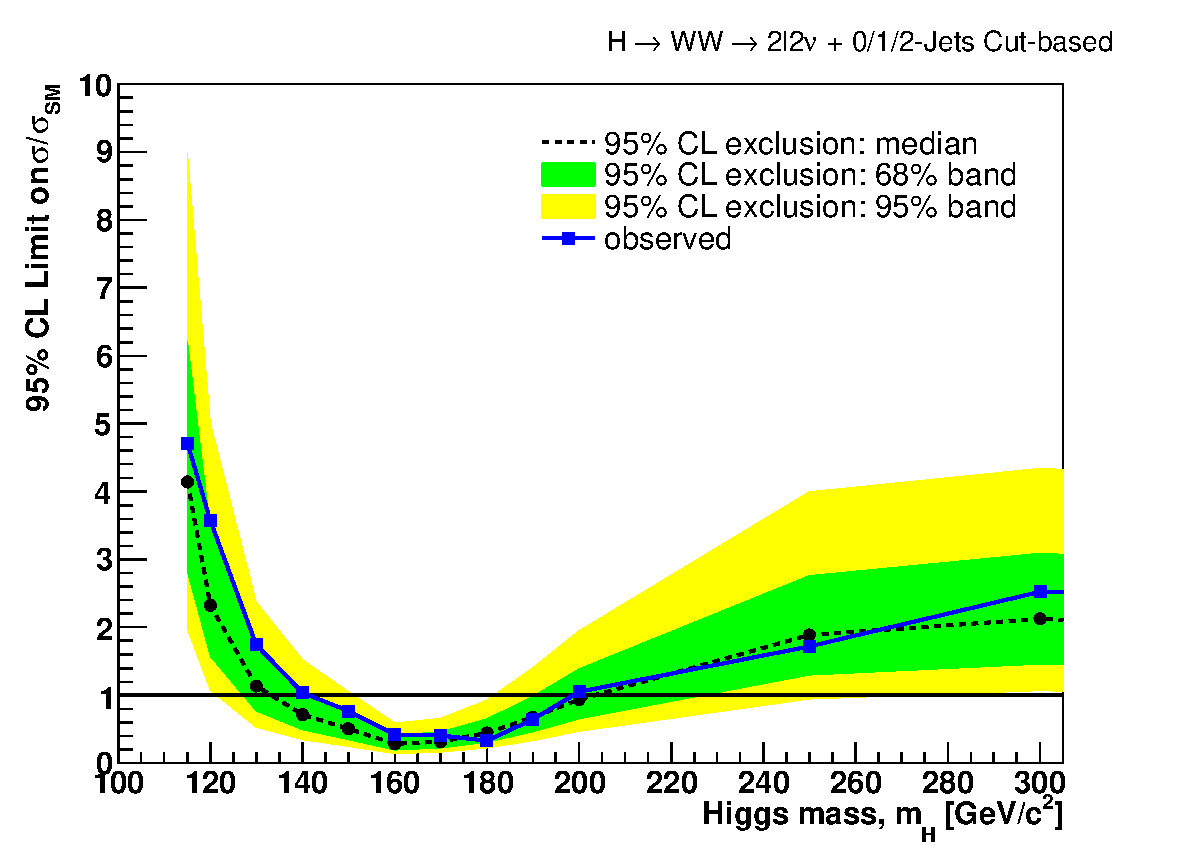
\includegraphics[width=0.48\textwidth]{lp_figures/limits_nj_cut_ana_v6_1500pb_LP_MTCUT80.pdf}}
\caption{Cut-based analysis upper limits at 95\% C.L. using data corresponding to 1.5~$\ifb$ applying the additional $m_T$ cut.
The limits are shown in 4 final states separately. \subref{subfig:0j_sf}: SF in 0 Jet bin;
\subref{subfig:0j_of}: OF in 0 Jet bin; \subref{subfig:1j_sf}: SF in 1 Jet bin;
\subref{subfig:1j_of}: OF in 1 Jet bin; \subref{subfig:2j}: 2 Jet bin; \subref{subfig:njcomb}: 0/1/2 Jets combined; }
\label{fig:limits_lp_mtcut80_cut}
\end{figure}
%%%%%%%%%%%%%%%%%%%%%%%%%%%%%%
\clearpage
\subsubsection{MVA-Based with Additional Transverse Mass Requirement}
\begin{figure}[!htbp]
\centering
\subfigure[]{
\centering
\label{subfig:0j_sf}
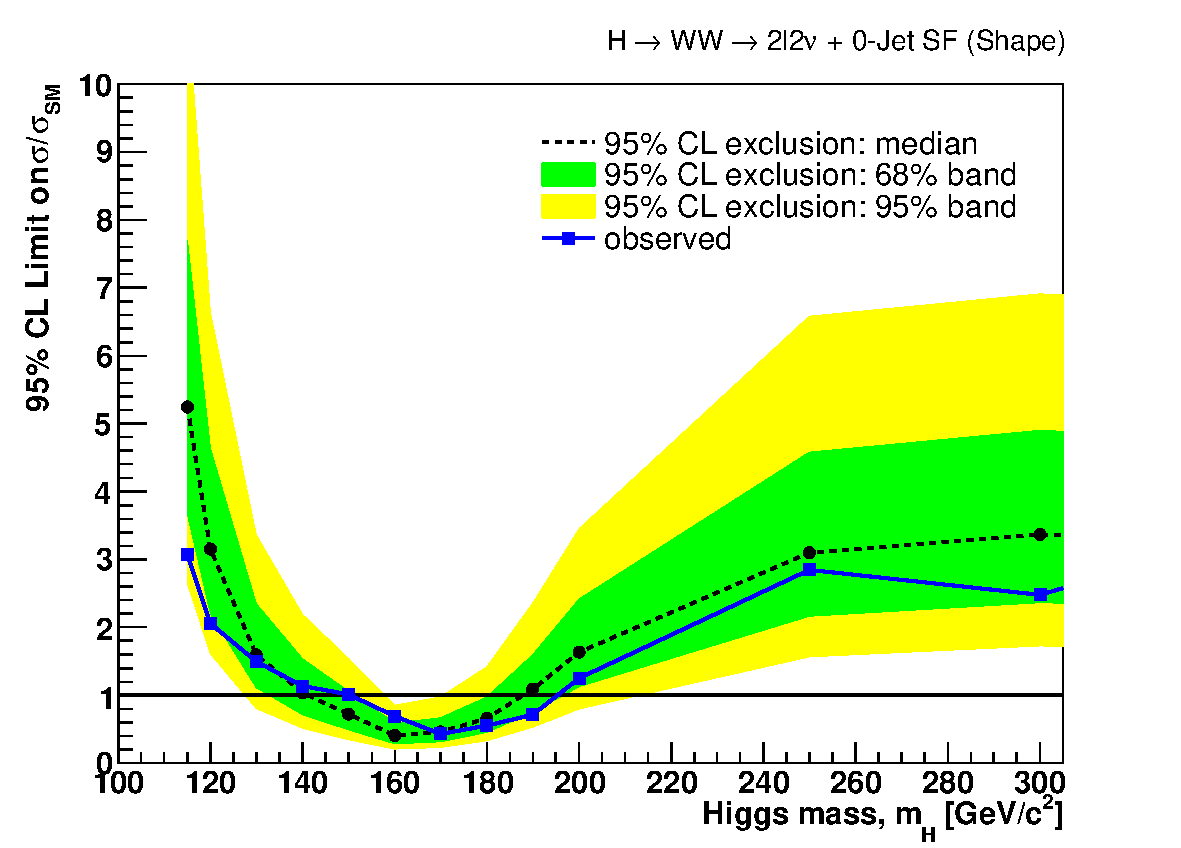
\includegraphics[width=0.48\textwidth]{lp_figures/limits_0j_sf_shape_ana_v6_1500pb_LP_MTCUT80.pdf}
}
\subfigure[]{
\centering
\label{subfig:0j_of}
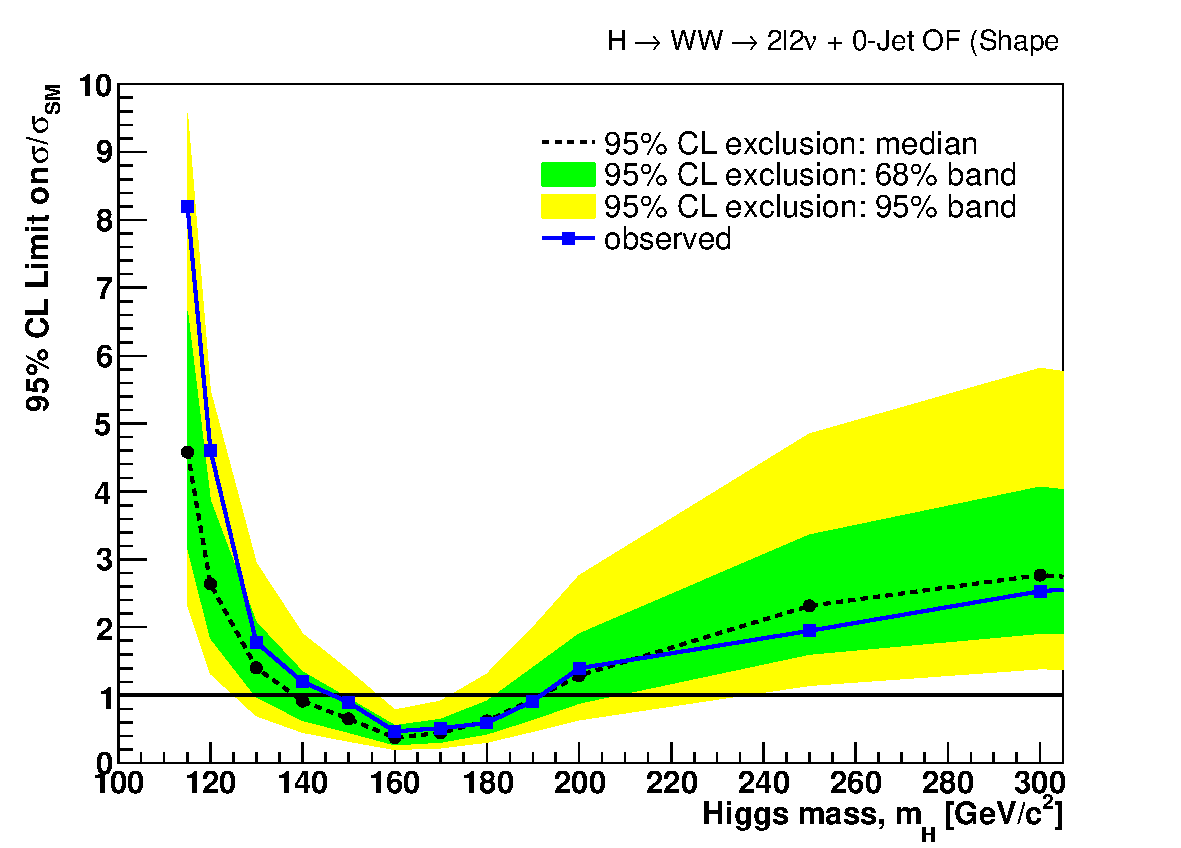
\includegraphics[width=0.48\textwidth]{lp_figures/limits_0j_of_shape_ana_v6_1500pb_LP_MTCUT80.pdf}
}
\subfigure[]{
\centering
\label{subfig:1j_sf}
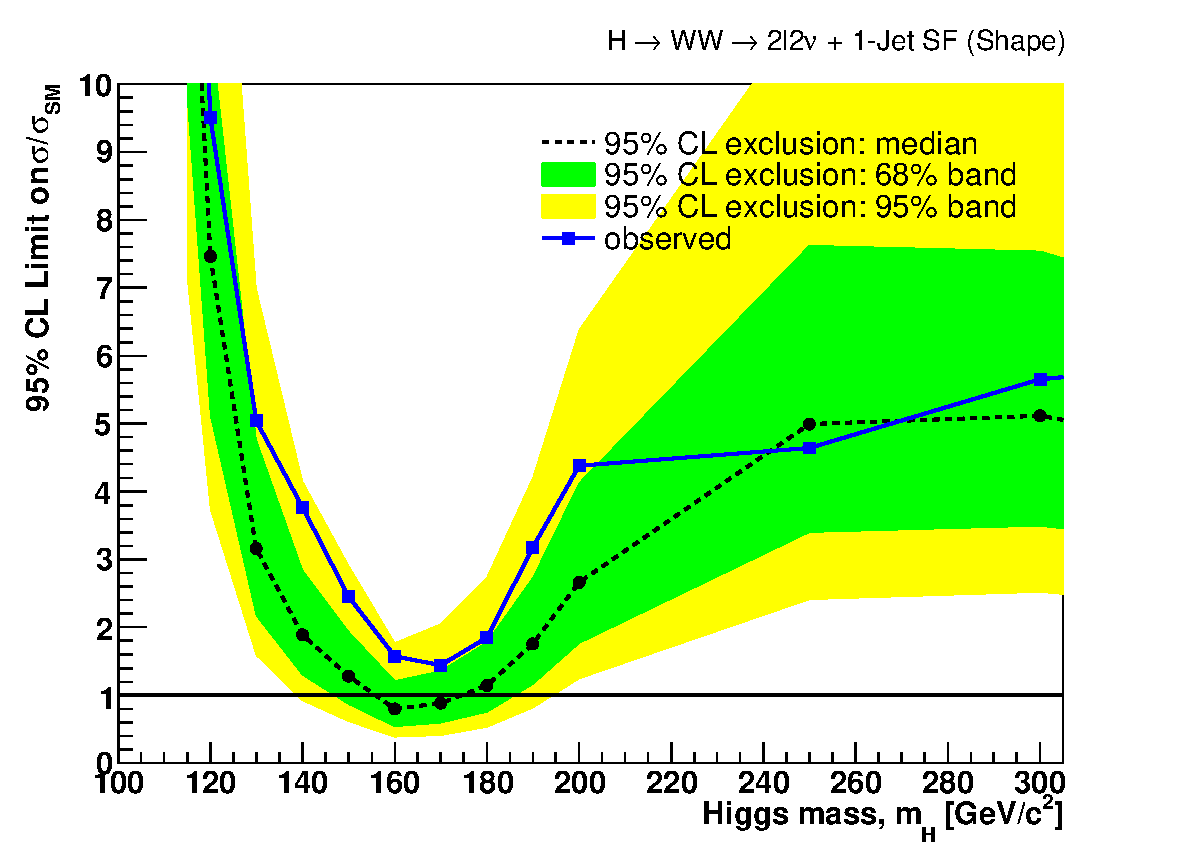
\includegraphics[width=0.48\textwidth]{lp_figures/limits_1j_sf_shape_ana_v6_1500pb_LP_MTCUT80.pdf}
}
\subfigure[]{
\centering
\label{subfig:1j_of}
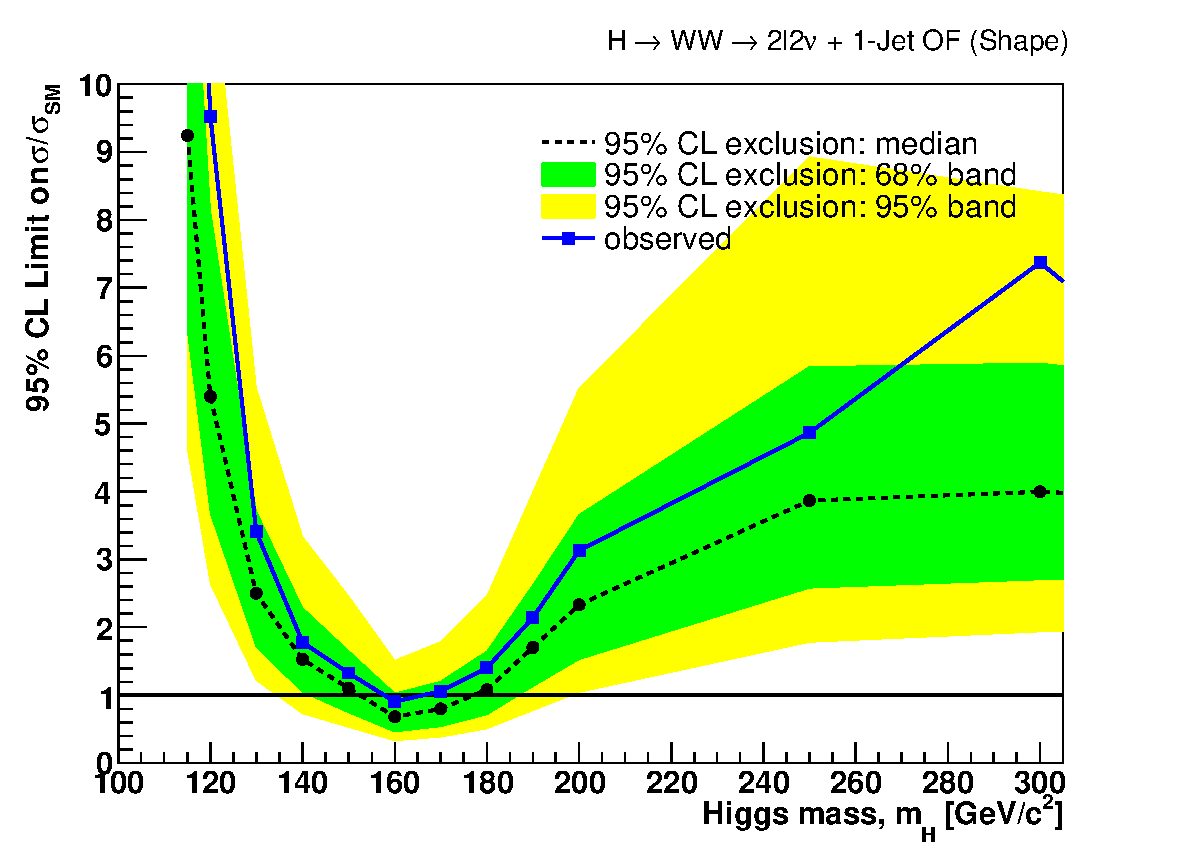
\includegraphics[width=0.48\textwidth]{lp_figures/limits_1j_of_shape_ana_v6_1500pb_LP_MTCUT80.pdf}
}
\subfigure[]{
\centering
\label{subfig:nj}
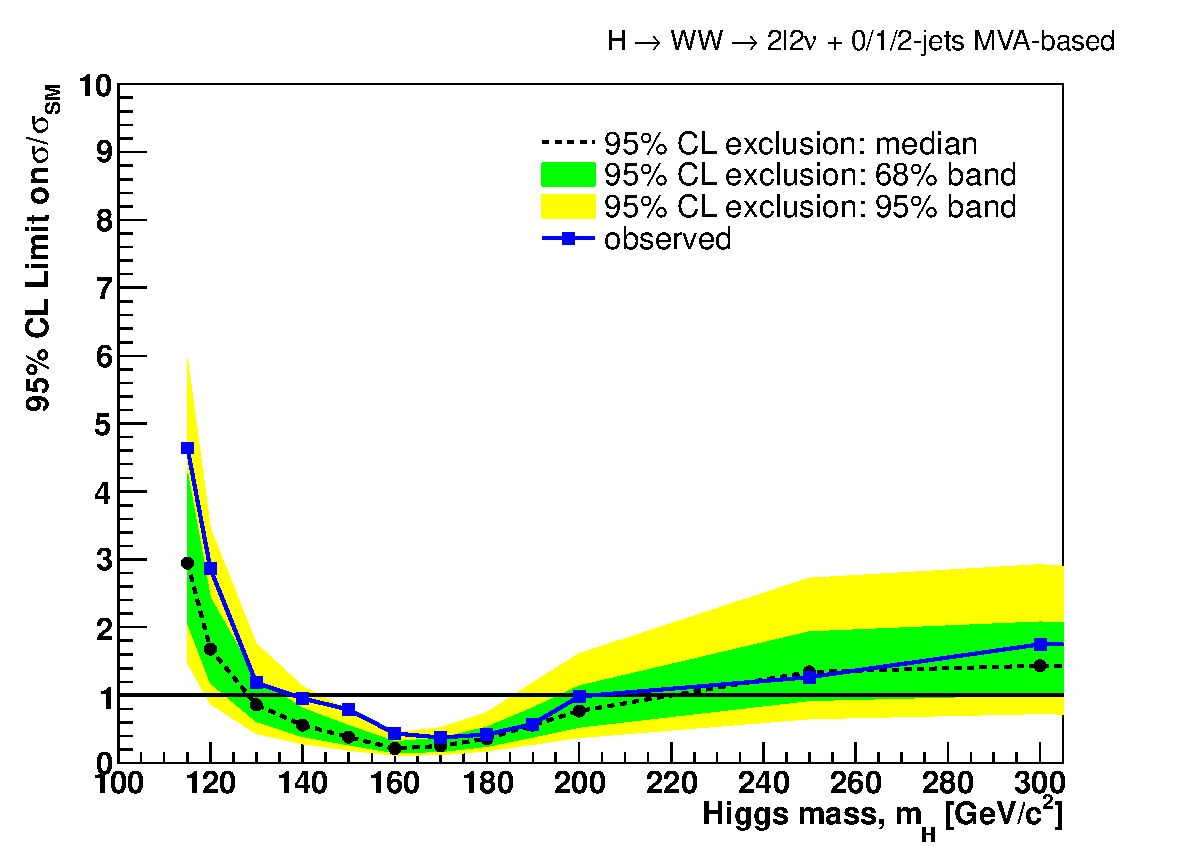
\includegraphics[width=0.48\textwidth]{lp_figures/limits_nj_shape_ana_v6_1500pb_LP_MTCUT80.pdf}
}
\caption{Multivariate based analysis upper limits at 95\% C.L. using data corresponding to 1.5~$\ifb$,
applying the additional $m_T$ cut.
The limits are shown in 4 final states separately. \subref{subfig:0j_sf}: SF in 0 Jet bin;
\subref{subfig:0j_of}: OF in 0 Jet bin; \subref{subfig:1j_sf}: SF in 1 Jet bin;
\subref{subfig:1j_of}: OF in 1 Jet bin; \subref{subfig:nj}: 0/1/2 Jets combined;
}
\label{fig:limits_lp_mtcut80_shape}
\end{figure}

%%%%%%%%%%%%%%%%%%%%%%%%%%%%%%
%
%
%
\pagebreak
\clearpage
\subsection{Tabulated Limits}
\subsubsection{EPS Dataset}
We report the upper limits obtained using the data with the run number
$<170826$ ( referred to as the EPS data) in the 0 and 1 jet bins separating the
same flavor ($ee/\mu\mu$) and opposite flavor ($e\mu$) final states.
The results tabulated in
Table~\ref{tab:limits_eps_cut}-\ref{tab:limits_eps_shape} respectively.

%%%%%%%%%%%%%%%%%%%%%%%%%%%%%%
\begin{table}
\begin{center}
\begin{tabular}{c c c c c}
\hline\hline
 $m_H$ (GeV) & Observed & Median Expected & 68\% C.L. Band & 95\% C.L. Band \\ \hline
\hline
\multicolumn{5}{c} {0-Jet Bin Same Flavor} \\
\hline
115 & 4.1 & 8.8 & [5.7, 15.4] & [4.0, 36.0] \\
120 & 4.1 & 5.0 & [3.2, 8.4] & [2.3, 17.6] \\
130 & 2.5 & 2.3 & [1.5, 3.4] & [1.0, 5.4] \\
140 & 1.6 & 1.5 & [1.0, 2.2] & [0.7, 3.3] \\
150 & 1.8 & 1.0 & [0.7, 1.5] & [0.5, 2.4] \\
160 & 1.0 & 0.6 & [0.4, 0.9] & [0.3, 1.6] \\
170 & 1.0 & 0.7 & [0.5, 1.0] & [0.3, 1.6] \\
180 & 0.6 & 1.0 & [0.7, 1.5] & [0.5, 2.2] \\
190 & 1.6 & 1.5 & [1.0, 2.1] & [0.7, 3.1] \\
200 & 2.1 & 2.2 & [1.6, 3.3] & [1.1, 4.6] \\
250 & 3.3 & 5.8 & [4.0, 8.5] & [3.0, 12.2] \\
300 & 4.3 & 5.5 & [3.9, 8.3] & [2.8, 11.9] \\
\hline
\multicolumn{5}{c} {0-Jet Bin Opposite Flavor} \\
\hline
115 & 7.6 & 6.6 & [4.5, 9.8] & [3.2, 14.4] \\
120 & 4.9 & 3.8 & [2.6, 5.7] & [1.9, 8.2] \\
130 & 2.8 & 1.9 & [1.3, 2.9] & [1.0, 4.2] \\
140 & 1.5 & 1.3 & [0.9, 1.8] & [0.6, 2.6] \\
150 & 0.9 & 1.0 & [0.7, 1.5] & [0.5, 2.2] \\
160 & 0.5 & 0.5 & [0.4, 0.8] & [0.3, 1.2] \\
170 & 0.7 & 0.7 & [0.5, 1.0] & [0.3, 1.4] \\
180 & 0.9 & 0.9 & [0.7, 1.4] & [0.5, 2.0] \\
190 & 1.4 & 1.3 & [0.9, 2.0] & [0.7, 2.8] \\
200 & 2.3 & 1.9 & [1.3, 2.8] & [1.0, 4.2] \\
250 & 3.1 & 3.9 & [2.8, 5.8] & [2.0, 8.2] \\
300 & 3.8 & 4.5 & [3.1, 6.6] & [2.3, 9.5] \\
\hline
\multicolumn{5}{c} {1-Jet Bin Same Flavor} \\
\hline
115 & 19.7 & 17.7 & [11.4, 26.5] & [8.6, 43.9] \\
120 & 12.4 & 9.4 & [6.4, 15.3] & [4.7, 27.8] \\
130 & 8.3 & 4.6 & [3.1, 7.2] & [2.1, 14.5] \\
140 & 5.7 & 2.7 & [1.7, 4.1] & [1.2, 7.0] \\
150 & 4.2 & 2.1 & [1.3, 3.2] & [1.0, 5.2] \\
160 & 2.3 & 1.1 & [0.8, 1.8] & [0.6, 2.7] \\
170 & 2.7 & 1.4 & [1.0, 2.1] & [0.7, 3.2] \\
180 & 2.9 & 1.8 & [1.3, 2.6] & [0.9, 3.8] \\
190 & 4.3 & 2.6 & [1.7, 4.0] & [1.3, 6.1] \\
200 & 6.5 & 4.0 & [2.7, 6.0] & [2.0, 9.4] \\
250 & 11.2 & 8.6 & [6.0, 13.2] & [4.4, 19.7] \\
300 & 12.1 & 8.7 & [6.0, 13.1] & [4.3, 19.5] \\
\hline
\multicolumn{5}{c} {1-Jet Bin Opposite Flavor} \\
\hline
115 & 19.4 & 10.2 & [6.9, 15.4] & [5.1, 22.9] \\
120 & 10.4 & 6.0 & [4.0, 8.9] & [3.0, 13.0] \\
130 & 4.1 & 3.2 & [2.1, 4.7] & [1.5, 7.2] \\
140 & 2.2 & 2.0 & [1.4, 3.0] & [1.0, 4.6] \\
150 & 1.6 & 1.6 & [1.1, 2.3] & [0.8, 3.5] \\
160 & 1.1 & 1.0 & [0.6, 1.4] & [0.5, 2.1] \\
170 & 1.2 & 1.2 & [0.8, 1.7] & [0.6, 2.7] \\
180 & 1.6 & 1.6 & [1.1, 2.5] & [0.9, 3.6] \\
190 & 2.1 & 2.6 & [1.8, 3.8] & [1.3, 5.6] \\
200 & 3.1 & 3.2 & [2.2, 4.8] & [1.6, 7.1] \\
250 & 6.2 & 6.1 & [4.2, 9.1] & [3.1, 13.6] \\
300 & 7.8 & 6.9 & [4.8, 10.4] & [3.5, 15.2] \\
\hline\hline
\end{tabular}
\end{center}
\caption{Cut based upper limits at 95\% C.L. in 0 and 1 Jet final state,
using the EPS data (run $<$ 170826) corresponding to  1.1~$\ifb$.}
\label{tab:limits_eps_cut}
\end{table}
%%%%%%%%%%%%%%%%%%%%%%%%%%%%%%
%%%%%%%%%%%%%%%%%%%%%%%%%%%%%%
\begin{table}
\begin{center}
\begin{tabular}{c c c c c}
\hline\hline
 $m_H$ (GeV) & Observed & Median Expected & 68\% C.L. Band & 95\% C.L. Band \\ \hline
\hline
\multicolumn{5}{c} {0-Jet Bin Same Flavor} \\
\hline
115 & 3.7 & 6.0 & [4.2, 8.7] & [3.1, 12.6] \\
120 & 2.6 & 3.6 & [2.5, 5.2] & [1.8, 7.5] \\
130 & 2.1 & 1.8 & [1.2, 2.6] & [0.9, 3.7] \\
140 & 1.9 & 1.2 & [0.8, 1.7] & [0.6, 2.4] \\
150 & 1.5 & 0.8 & [0.6, 1.2] & [0.4, 1.7] \\
160 & 1.0 & 0.5 & [0.3, 0.7] & [0.2, 1.0] \\
170 & 0.7 & 0.5 & [0.4, 0.8] & [0.3, 1.1] \\
180 & 0.8 & 0.7 & [0.5, 1.1] & [0.4, 1.6] \\
190 & 1.0 & 1.2 & [0.8, 1.8] & [0.6, 2.6] \\
200 & 1.5 & 1.8 & [1.3, 2.7] & [0.9, 3.9] \\
250 & 3.0 & 3.5 & [2.5, 5.2] & [1.8, 7.5] \\
300 & 3.5 & 3.9 & [2.8, 5.8] & [2.0, 8.2] \\
\hline
\multicolumn{5}{c} {0-Jet Bin Opposite Flavor} \\
\hline
115 & 10.9 & 5.0 & [3.4, 7.3] & [2.5, 10.5] \\
120 & 5.9 & 2.9 & [2.0, 4.3] & [1.4, 5.9] \\
130 & 2.4 & 1.5 & [1.1, 2.2] & [0.8, 3.2] \\
140 & 1.3 & 1.0 & [0.7, 1.4] & [0.5, 2.1] \\
150 & 1.1 & 0.7 & [0.5, 1.0] & [0.4, 1.5] \\
160 & 0.7 & 0.4 & [0.3, 0.6] & [0.2, 0.9] \\
170 & 0.7 & 0.5 & [0.3, 0.7] & [0.3, 1.1] \\
180 & 0.8 & 0.7 & [0.5, 1.0] & [0.4, 1.5] \\
190 & 1.3 & 1.1 & [0.7, 1.6] & [0.5, 2.2] \\
200 & 1.8 & 1.4 & [1.0, 2.1] & [0.7, 3.0] \\
250 & 2.2 & 2.6 & [1.8, 3.7] & [1.3, 5.3] \\
300 & 2.7 & 3.2 & [2.2, 4.7] & [1.6, 6.6] \\
\hline
\multicolumn{5}{c} {1-Jet Bin Same Flavor} \\
\hline
115 & 24.4 & 14.8 & [10.3, 21.7] & [7.5, 30.8] \\
120 & 11.5 & 8.3 & [5.7, 12.2] & [4.2, 17.9] \\
130 & 6.5 & 3.7 & [2.5, 5.5] & [1.8, 7.8] \\
140 & 4.1 & 2.1 & [1.5, 3.1] & [1.1, 4.6] \\
150 & 2.6 & 1.4 & [1.0, 2.2] & [0.7, 3.2] \\
160 & 1.6 & 0.9 & [0.6, 1.3] & [0.4, 2.0] \\
170 & 1.8 & 1.0 & [0.7, 1.5] & [0.5, 2.3] \\
180 & 2.5 & 1.3 & [0.8, 1.9] & [0.6, 2.9] \\
190 & 4.0 & 2.0 & [1.3, 3.0] & [0.9, 4.6] \\
200 & 5.8 & 3.0 & [2.0, 4.6] & [1.4, 6.9] \\
250 & 6.7 & 5.6 & [3.8, 8.4] & [2.7, 12.5] \\
300 & 7.2 & 5.8 & [4.0, 8.5] & [2.9, 12.2] \\
\hline
\multicolumn{5}{c} {1-Jet Bin Opposite Flavor} \\
\hline
115 & 15.8 & 8.7 & [6.1, 12.8] & [4.4, 18.3] \\
120 & 8.3 & 5.5 & [3.8, 8.0] & [2.8, 11.6] \\
130 & 3.8 & 2.8 & [1.9, 4.2] & [1.4, 6.0] \\
140 & 2.1 & 1.7 & [1.1, 2.5] & [0.8, 3.6] \\
150 & 1.5 & 1.2 & [0.9, 1.9] & [0.6, 2.7] \\
160 & 1.0 & 0.8 & [0.5, 1.2] & [0.4, 1.7] \\
170 & 1.2 & 0.9 & [0.6, 1.4] & [0.4, 2.0] \\
180 & 1.5 & 1.2 & [0.8, 1.8] & [0.6, 2.8] \\
190 & 2.0 & 1.9 & [1.2, 2.9] & [0.9, 4.4] \\
200 & 2.9 & 2.5 & [1.7, 3.9] & [1.2, 5.9] \\
250 & 5.1 & 4.2 & [2.8, 6.3] & [1.9, 9.4] \\
300 & 4.9 & 4.3 & [3.0, 6.4] & [2.1, 9.3] \\
\hline\hline
\end{tabular}
\end{center}
\caption{Multivariate based upper limits at 95\% C.L. in 0 and 1 Jet final state,
using the EPS data (run $<$ 170826) corresponding to  1.1~$\ifb$.}
\label{tab:limits_eps_shape}
\end{table}
%%%%%%%%%%%%%%%%%%%%%%%%%%%%%%

%
%
%
\pagebreak
\clearpage
\subsubsection{post-EPS Dataset}
We report the upper limits obtained using the data with the run number $>=170826$ ( referred to
as the post-EPS data) in the 0 and 1 jet bins separating the
same flavor ($ee/\mu\mu$) and opposite flavor ($e\mu$) final states.
The results are tabulated in
Table~\ref{tab:limits_posteps_cut}-\ref{tab:limits_posteps_shape} respectively.

%%%%%%%%%%%%%%%%%%%%%%%%%%%%%%
\begin{table}
\begin{center}
\begin{tabular}{c c c c c}
\hline\hline
 $m_H$ (GeV) & Observed & Median Expected & 68\% C.L. Band & 95\% C.L. Band \\ \hline
\hline
\multicolumn{5}{c} {0-Jet Bin Same Flavor} \\
\hline
115 & 14.3 & 12.9 & [8.8, 21.4] & [6.8, 43.3] \\
120 & 6.9 & 7.6 & [5.0, 11.9] & [3.6, 21.3] \\
130 & 3.1 & 3.4 & [2.3, 5.2] & [1.7, 7.5] \\
140 & 1.8 & 2.3 & [1.6, 3.4] & [1.2, 5.0] \\
150 & 1.1 & 1.7 & [1.1, 2.5] & [1.0, 3.8] \\
160 & 0.6 & 1.0 & [0.7, 1.5] & [0.6, 2.2] \\
170 & 0.6 & 1.2 & [0.9, 1.7] & [0.6, 2.5] \\
180 & 1.0 & 1.9 & [1.4, 2.5] & [1.0, 3.7] \\
190 & 1.6 & 2.6 & [1.8, 3.9] & [1.4, 5.3] \\
200 & 3.2 & 3.8 & [2.8, 5.4] & [2.1, 7.9] \\
250 & 8.1 & 9.5 & [6.9, 14.4] & [5.2, 20.2] \\
300 & 9.5 & 9.5 & [7.0, 14.4] & [5.1, 20.2] \\
\hline
\multicolumn{5}{c} {0-Jet Bin Opposite Flavor} \\
\hline
115 & 9.6 & 10.4 & [7.2, 15.1] & [5.2, 22.3] \\
120 & 4.9 & 5.8 & [4.1, 8.6] & [3.0, 12.8] \\
130 & 2.6 & 3.0 & [2.1, 4.5] & [1.5, 6.3] \\
140 & 1.6 & 2.0 & [1.4, 2.9] & [1.1, 4.1] \\
150 & 1.9 & 1.7 & [1.3, 2.5] & [0.9, 3.7] \\
160 & 0.9 & 1.0 & [0.7, 1.5] & [0.6, 2.2] \\
170 & 0.7 & 1.3 & [0.9, 1.7] & [0.6, 2.6] \\
180 & 1.2 & 1.6 & [1.2, 2.5] & [1.0, 3.3] \\
190 & 1.6 & 2.4 & [1.6, 3.4] & [1.2, 4.7] \\
200 & 2.4 & 3.4 & [2.4, 4.8] & [1.7, 6.6] \\
250 & 7.7 & 6.8 & [4.8, 9.6] & [3.5, 13.7] \\
300 & 10.4 & 8.1 & [5.4, 11.7] & [4.2, 16.0] \\
\hline
\multicolumn{5}{c} {1-Jet Bin Same Flavor} \\
\hline
115 & 37.5 & 31.2 & [21.4, 50.3] & [17.2, 74.9] \\
120 & 19.1 & 16.3 & [11.7, 25.6] & [9.4, 42.9] \\
130 & 7.5 & 8.7 & [6.3, 13.2] & [4.5, 21.9] \\
140 & 5.2 & 5.1 & [3.5, 7.2] & [2.5, 11.4] \\
150 & 4.5 & 3.7 & [2.6, 5.4] & [2.1, 9.0] \\
160 & 2.9 & 2.4 & [1.6, 3.4] & [1.3, 5.1] \\
170 & 3.1 & 2.5 & [2.0, 3.8] & [1.6, 5.3] \\
180 & 3.0 & 3.1 & [2.4, 4.5] & [1.9, 7.0] \\
190 & 3.3 & 4.7 & [3.3, 6.6] & [2.4, 9.9] \\
200 & 4.9 & 7.0 & [4.9, 10.8] & [4.0, 15.4] \\
250 & 9.2 & 15.3 & [11.0, 23.8] & [9.1, 34.2] \\
300 & 16.0 & 15.9 & [11.5, 21.6] & [8.5, 30.9] \\
\hline
\multicolumn{5}{c} {1-Jet Bin Opposite Flavor} \\
\hline
115 & 41.3 & 19.6 & [14.2, 29.5] & [10.4, 41.5] \\
120 & 24.8 & 11.2 & [7.4, 16.5] & [5.6, 24.4] \\
130 & 11.4 & 5.6 & [3.7, 8.2] & [3.1, 11.5] \\
140 & 6.4 & 3.7 & [2.7, 5.6] & [2.0, 8.0] \\
150 & 4.2 & 3.0 & [2.1, 4.2] & [1.5, 6.1] \\
160 & 2.6 & 1.8 & [1.2, 2.6] & [1.0, 3.9] \\
170 & 2.6 & 2.2 & [1.7, 3.2] & [1.4, 5.0] \\
180 & 2.6 & 3.2 & [2.2, 4.6] & [1.7, 6.2] \\
190 & 3.7 & 4.4 & [3.2, 6.6] & [2.4, 9.3] \\
200 & 6.3 & 5.5 & [4.1, 8.1] & [3.1, 12.2] \\
250 & 17.0 & 9.9 & [7.0, 15.2] & [5.4, 21.8] \\
300 & 21.4 & 11.2 & [8.4, 17.3] & [6.0, 24.9] \\
\hline\hline
\end{tabular}
\end{center}
\caption{Cut-based upper limits at 95\% C.L. in 0 and 1 Jet final state,
using the post-EPS data (run $>=$ 170826) corresponding to  0.4~$\ifb$.}
\label{tab:limits_posteps_cut}
\end{table}
%%%%%%%%%%%%%%%%%%%%%%%%%%%%%%
%%%%%%%%%%%%%%%%%%%%%%%%%%%%%%
\begin{table}
\begin{center}
\begin{tabular}{c c c c c}
\hline\hline
 $m_H$ (GeV) & Observed & Median Expected & 68\% C.L. Band & 95\% C.L. Band \\ \hline
\hline
\multicolumn{5}{c} {0-Jet Bin Same Flavor} \\
\hline
115 & 10.2 & 10.2 & [7.3, 14.7] & [5.4, 20.9] \\
120 & 4.8 & 5.9 & [4.2, 8.5] & [3.1, 12.4] \\
130 & 2.7 & 2.8 & [2.0, 4.1] & [1.5, 5.9] \\
140 & 1.2 & 1.8 & [1.2, 2.6] & [0.9, 3.7] \\
150 & 0.8 & 1.2 & [0.9, 1.8] & [0.6, 2.6] \\
160 & 0.5 & 0.8 & [0.6, 1.1] & [0.4, 1.6] \\
170 & 0.5 & 0.9 & [0.6, 1.2] & [0.4, 1.8] \\
180 & 0.8 & 1.2 & [0.8, 1.8] & [0.6, 2.5] \\
190 & 1.5 & 1.9 & [1.3, 2.8] & [1.0, 4.1] \\
200 & 2.6 & 2.9 & [2.0, 4.2] & [1.5, 6.1] \\
250 & 6.9 & 5.9 & [4.1, 8.6] & [3.0, 12.3] \\
300 & 5.2 & 6.7 & [4.7, 9.8] & [3.6, 14.0] \\
\hline
\multicolumn{5}{c} {0-Jet Bin Opposite Flavor} \\
\hline
115 & 9.8 & 7.9 & [5.5, 11.5] & [4.1, 16.5] \\
120 & 4.8 & 4.7 & [3.3, 6.9] & [2.4, 9.8] \\
130 & 3.3 & 2.4 & [1.7, 3.6] & [1.2, 5.2] \\
140 & 2.0 & 1.6 & [1.1, 2.4] & [0.8, 3.4] \\
150 & 1.8 & 1.2 & [0.8, 1.7] & [0.6, 2.4] \\
160 & 0.9 & 0.8 & [0.5, 1.1] & [0.4, 1.6] \\
170 & 0.9 & 0.9 & [0.6, 1.2] & [0.4, 1.8] \\
180 & 1.0 & 1.2 & [0.8, 1.7] & [0.6, 2.4] \\
190 & 1.5 & 1.7 & [1.2, 2.5] & [0.8, 3.5] \\
200 & 1.9 & 2.3 & [1.6, 3.4] & [1.2, 4.9] \\
250 & 4.9 & 4.3 & [3.0, 6.2] & [2.2, 8.9] \\
300 & 6.4 & 5.2 & [3.7, 7.7] & [2.7, 10.9] \\
\hline
\multicolumn{5}{c} {1-Jet Bin Same Flavor} \\
\hline
115 & 26.5 & 26.2 & [18.5, 38.7] & [14.1, 55.0] \\
120 & 13.4 & 15.0 & [10.5, 22.0] & [7.9, 32.3] \\
130 & 6.5 & 6.5 & [4.6, 9.6] & [3.4, 13.9] \\
140 & 4.2 & 3.8 & [2.6, 5.6] & [1.9, 8.2] \\
150 & 2.5 & 2.5 & [1.7, 3.7] & [1.3, 5.5] \\
160 & 1.5 & 1.6 & [1.1, 2.4] & [0.8, 3.4] \\
170 & 1.4 & 1.7 & [1.2, 2.5] & [0.9, 3.7] \\
180 & 1.6 & 2.1 & [1.4, 3.1] & [1.0, 4.5] \\
190 & 2.4 & 3.2 & [2.2, 4.7] & [1.6, 7.0] \\
200 & 3.3 & 4.7 & [3.2, 7.0] & [2.3, 10.3] \\
250 & 5.9 & 9.1 & [6.3, 13.6] & [4.7, 19.9] \\
300 & 8.3 & 9.8 & [6.9, 14.4] & [5.1, 20.9] \\
\hline
\multicolumn{5}{c} {1-Jet Bin Opposite Flavor} \\
\hline
115 & 20.2 & 15.9 & [11.1, 23.5] & [8.2, 33.6] \\
120 & 11.0 & 9.7 & [6.7, 14.3] & [4.9, 20.9] \\
130 & 4.9 & 4.7 & [3.3, 7.1] & [2.4, 10.3] \\
140 & 3.2 & 2.9 & [2.0, 4.2] & [1.4, 6.0] \\
150 & 2.1 & 2.0 & [1.4, 3.0] & [1.0, 4.4] \\
160 & 1.7 & 1.4 & [1.0, 2.0] & [0.7, 3.0] \\
170 & 1.7 & 1.5 & [1.0, 2.3] & [0.8, 3.4] \\
180 & 2.1 & 2.0 & [1.3, 2.9] & [1.0, 4.4] \\
190 & 3.5 & 2.9 & [2.0, 4.4] & [1.4, 6.6] \\
200 & 4.7 & 3.9 & [2.6, 5.9] & [1.9, 8.8] \\
250 & 7.1 & 6.4 & [4.3, 9.6] & [3.1, 14.1] \\
300 & 12.3 & 7.1 & [4.9, 10.4] & [3.6, 15.4] \\
\hline\hline
\end{tabular}
\end{center}
\caption{Multivariate based upper limits at 95\% C.L. in 0 and 1 Jet final state,
using the post-EPS data (run $>=$ 170826) corresponding to  0.4~$\ifb$.}
\label{tab:limits_posteps_shape}
\end{table}
%%%%%%%%%%%%%%%%%%%%%%%%%%%%%%


%
%
%
\pagebreak
\clearpage

\subsubsection{LP Dataset}
\label{app:lp_limits_default}
In this section we report the observed and expected upper limits
correspoinding to 1.5~$\ifb$ LP2011 dataset.
The results are tabulated in Table~\ref{tab:limits_lp}
and Table~\ref{tab:limits_lp_shape_splitflavor}.

%%%%%%%%%%%%%%%%%%%%%%%%%%%%%%
\begin{table}
\begin{center}
\begin{tabular}{c c c c c}
\hline\hline
 $m_H$ (GeV) & Observed & Median Expected & 68\% C.L. Band & 95\% C.L. Band \\ \hline
\hline
\multicolumn{5}{c} {0/1/2-Jets Cut-Based}\\
\hline
115 & 5.6 & 4.3 & [2.8, 6.5] & [1.9, 9.4] \\
120 & 3.9 & 2.5 & [1.7, 3.7] & [1.1, 5.4] \\
130 & 1.9 & 1.2 & [0.8, 1.8] & [0.6, 2.6] \\
140 & 1.0 & 0.7 & [0.5, 1.1] & [0.3, 1.5] \\
150 & 0.8 & 0.5 & [0.4, 0.8] & [0.3, 1.1] \\
160 & 0.4 & 0.3 & [0.2, 0.4] & [0.1, 0.6] \\
170 & 0.4 & 0.3 & [0.2, 0.5] & [0.2, 0.7] \\
180 & 0.3 & 0.5 & [0.3, 0.7] & [0.2, 1.0] \\
190 & 0.7 & 0.7 & [0.5, 1.0] & [0.3, 1.4] \\
200 & 1.1 & 1.0 & [0.7, 1.4] & [0.5, 2.1] \\
250 & 1.8 & 1.9 & [1.3, 2.8] & [0.9, 3.9] \\
300 & 2.6 & 2.1 & [1.5, 3.1] & [1.1, 4.4] \\
\hline
\multicolumn{5}{c} {0/1/-Jets Multivariate Based combined with 2-Jet Cut Based}\\
\hline
115 & 6.1 & 2.8 & [1.9, 4.1] & [1.4, 5.9]  \\
120 & 2.8 & 1.6 & [1.1, 2.3] & [0.8, 3.3]  \\
130 & 1.7 & 0.8 & [0.6, 1.2] & [0.4, 1.7]  \\
140 & 1.1 & 0.5 & [0.4, 0.7] & [0.3, 1.1]  \\
150 & 0.8 & 0.4 & [0.3, 0.5] & [0.2, 0.7]  \\
160 & 0.5 & 0.2 & [0.1, 0.3] & [0.1, 0.4]  \\
170 & 0.4 & 0.3 & [0.2, 0.4] & [0.1, 0.5]  \\
180 & 0.4 & 0.4 & [0.3, 0.5] & [0.2, 0.7]  \\
190 & 0.6 & 0.5 & [0.4, 0.8] & [0.3, 1.1]  \\
200 & 1.0 & 0.8 & [0.5, 1.1] & [0.4, 1.6]  \\
250 & 1.3 & 1.3 & [0.9, 1.9] & [0.6, 2.7]  \\
300 & 1.7 & 1.4 & [1.0, 2.1] & [0.7, 2.9]  \\
\hline\hline
\end{tabular}
\end{center}
\caption{Upper limits at 95\% C.L. in 0, 1 and 2 Jet final states for both
cut-based and multivariate based analyses.
The results correspond to the 1.5~$\ifb$ data.
}
\label{tab:limits_lp}
\end{table}
%%%%%%%%%%%%%%%%%%%%%%%%%%%%%%
%%%%%%%%%%%%%%%%%%%%%%%%%%%%%%
\begin{table}
\begin{center}
\begin{tabular}{c c c c c}
\hline\hline
 $m_H$ (GeV) & Observed & Median Expected & 68\% C.L. Band & 95\% C.L. Band \\ \hline
\hline
\multicolumn{5}{c} {0-Jet Bin Same Flavor} \\
\hline
115 & 4.2 & 7.7 & [4.9, 13.9] & [3.4, 35.6] \\
120 & 3.7 & 4.4 & [2.8, 7.6] & [2.0, 16.9] \\
130 & 2.1 & 2.0 & [1.3, 3.1] & [0.9, 4.9] \\
140 & 1.2 & 1.3 & [0.9, 2.0] & [0.6, 3.0] \\
150 & 1.2 & 0.9 & [0.6, 1.3] & [0.4, 2.3] \\
160 & 0.6 & 0.5 & [0.3, 0.7] & [0.3, 1.1] \\
170 & 0.6 & 0.6 & [0.4, 0.9] & [0.3, 1.4] \\
180 & 0.4 & 0.9 & [0.6, 1.3] & [0.4, 1.9] \\
190 & 1.1 & 1.3 & [0.9, 1.9] & [0.6, 2.7] \\
200 & 1.7 & 1.9 & [1.3, 2.9] & [0.9, 4.1] \\
250 & 2.8 & 5.0 & [3.4, 7.3] & [2.4, 10.3] \\
300 & 3.7 & 4.7 & [3.3, 7.0] & [2.3, 9.9] \\
\hline
\multicolumn{5}{c} {0-Jet Bin Opposite Flavor} \\
\hline
115 & 6.4 & 5.9 & [4.0, 9.0] & [2.8, 13.3] \\
120 & 3.9 & 3.4 & [2.3, 5.1] & [1.6, 7.6] \\
130 & 2.2 & 1.7 & [1.2, 2.6] & [0.8, 3.8] \\
140 & 1.2 & 1.1 & [0.8, 1.6] & [0.5, 2.4] \\
150 & 0.8 & 0.9 & [0.6, 1.3] & [0.4, 1.9] \\
160 & 0.4 & 0.5 & [0.3, 0.7] & [0.2, 1.0] \\
170 & 0.5 & 0.6 & [0.4, 0.8] & [0.3, 1.2] \\
180 & 0.7 & 0.8 & [0.6, 1.2] & [0.4, 1.7] \\
190 & 1.0 & 1.2 & [0.8, 1.7] & [0.6, 2.5] \\
200 & 1.7 & 1.7 & [1.2, 2.5] & [0.8, 3.6] \\
250 & 3.0 & 3.5 & [2.4, 5.2] & [1.7, 7.6] \\
300 & 3.9 & 3.9 & [2.7, 5.8] & [2.0, 8.3] \\
\hline
\multicolumn{5}{c} {1-Jet Bin Same Flavor} \\
\hline
115 & 17.8 & 14.9 & [10.0, 23.6] & [7.2, 39.8] \\
120 & 10.9 & 8.3 & [5.4, 13.4] & [3.8, 25.8] \\
130 & 6.4 & 4.1 & [2.6, 6.7] & [1.8, 14.5] \\
140 & 4.6 & 2.3 & [1.5, 3.6] & [1.1, 6.2] \\
150 & 3.5 & 1.8 & [1.2, 2.8] & [0.9, 4.9] \\
160 & 2.0 & 1.0 & [0.7, 1.6] & [0.5, 2.4] \\
170 & 2.2 & 1.2 & [0.8, 1.8] & [0.6, 2.7] \\
180 & 2.2 & 1.5 & [1.1, 2.3] & [0.8, 3.5] \\
190 & 3.1 & 2.2 & [1.5, 3.5] & [1.1, 5.5] \\
200 & 4.5 & 3.4 & [2.4, 5.2] & [1.7, 8.5] \\
250 & 7.2 & 7.6 & [5.2, 11.3] & [3.8, 16.8] \\
300 & 10.0 & 7.5 & [5.1, 11.3] & [3.7, 16.7] \\
\hline
\multicolumn{5}{c} {1-Jet Bin Opposite Flavor} \\
\hline
115 & 21.2 & 9.3 & [6.3, 13.6] & [4.5, 20.0] \\
120 & 12.0 & 5.3 & [3.6, 8.0] & [2.6, 12.1] \\
130 & 4.8 & 2.8 & [1.9, 4.2] & [1.4, 6.2] \\
140 & 2.5 & 1.8 & [1.2, 2.7] & [0.9, 4.1] \\
150 & 1.7 & 1.4 & [0.9, 2.1] & [0.7, 3.0] \\
160 & 1.1 & 0.8 & [0.6, 1.2] & [0.4, 1.9] \\
170 & 1.1 & 1.1 & [0.7, 1.6] & [0.5, 2.3] \\
180 & 1.3 & 1.4 & [0.9, 2.1] & [0.7, 3.1] \\
190 & 1.7 & 2.2 & [1.5, 3.4] & [1.1, 5.0] \\
200 & 2.9 & 2.8 & [1.9, 4.3] & [1.4, 6.4] \\
250 & 6.9 & 5.6 & [3.7, 8.3] & [2.6, 12.2] \\
300 & 8.9 & 6.1 & [4.1, 9.3] & [2.9, 13.5] \\
\hline\hline
\end{tabular}
\end{center}
\caption{Cut based upper limits at 95\% C.L. in 0 and 1 Jet final states
using data corresponding to 1.5~$\ifb$.}
\label{tab:limits_lp_cut_splitflavor}
\end{table}
%%%%%%%%%%%%%%%%%%%%%%%%%%%%%%
%%%%%%%%%%%%%%%%%%%%%%%%%%%%%%
\begin{table}
\begin{center}
\begin{tabular}{c c c c c}
\hline\hline
 $m_H$ (GeV) & Observed & Median Expected & 68\% C.L. Band & 95\% C.L. Band \\ \hline
\hline
\multicolumn{5}{c} {0-Jet Bin Same Flavor} \\
\hline
115 & 3.1 & 5.0 & [3.5, 7.4] & [2.6, 10.6] \\
120 & 2.0 & 3.1 & [2.1, 4.5] & [1.5, 6.4] \\
130 & 1.6 & 1.6 & [1.1, 2.3] & [0.8, 3.2] \\
140 & 1.3 & 1.0 & [0.7, 1.5] & [0.5, 2.1] \\
150 & 1.0 & 0.7 & [0.5, 1.0] & [0.3, 1.5] \\
160 & 0.6 & 0.4 & [0.3, 0.6] & [0.2, 0.9] \\
170 & 0.4 & 0.4 & [0.3, 0.7] & [0.2, 0.9] \\
180 & 0.5 & 0.7 & [0.4, 1.0] & [0.3, 1.4] \\
190 & 0.7 & 1.1 & [0.7, 1.6] & [0.5, 2.3] \\
200 & 1.3 & 1.6 & [1.1, 2.4] & [0.8, 3.5] \\
250 & 2.8 & 3.1 & [2.1, 4.5] & [1.6, 6.5] \\
300 & 2.5 & 3.4 & [2.3, 4.9] & [1.7, 7.2] \\
\hline
\multicolumn{5}{c} {0-Jet Bin Opposite Flavor} \\
\hline
115 & 9.0 & 4.3 & [3.0, 6.3] & [2.1, 9.2] \\
120 & 4.6 & 2.5 & [1.7, 3.7] & [1.3, 5.2] \\
130 & 2.2 & 1.3 & [0.9, 1.9] & [0.6, 2.7] \\
140 & 1.2 & 0.9 & [0.6, 1.2] & [0.4, 1.7] \\
150 & 1.1 & 0.6 & [0.4, 0.9] & [0.3, 1.3] \\
160 & 0.6 & 0.4 & [0.3, 0.5] & [0.2, 0.7] \\
170 & 0.6 & 0.4 & [0.3, 0.6] & [0.2, 0.9] \\
180 & 0.6 & 0.6 & [0.4, 0.9] & [0.3, 1.3] \\
190 & 1.0 & 0.9 & [0.6, 1.4] & [0.5, 2.0] \\
200 & 1.3 & 1.3 & [0.9, 1.9] & [0.6, 2.7] \\
250 & 2.0 & 2.3 & [1.6, 3.3] & [1.1, 4.7] \\
300 & 2.6 & 2.8 & [1.9, 4.0] & [1.4, 5.8] \\
\hline
\multicolumn{5}{c} {1-Jet Bin Same Flavor} \\
\hline
115 & 20.1 & 12.5 & [8.7, 18.4] & [6.3, 27.3] \\
120 & 9.6 & 7.2 & [4.9, 10.7] & [3.5, 15.4] \\
130 & 5.5 & 3.1 & [2.2, 4.6] & [1.6, 6.7] \\
140 & 3.8 & 1.9 & [1.3, 2.8] & [0.9, 4.1] \\
150 & 2.3 & 1.3 & [0.9, 1.9] & [0.6, 2.9] \\
160 & 1.4 & 0.8 & [0.5, 1.2] & [0.4, 1.7] \\
170 & 1.4 & 0.9 & [0.6, 1.4] & [0.4, 2.0] \\
180 & 1.9 & 1.1 & [0.7, 1.7] & [0.5, 2.6] \\
190 & 3.1 & 1.8 & [1.2, 2.7] & [0.8, 4.1] \\
200 & 4.3 & 2.7 & [1.8, 4.2] & [1.2, 6.5] \\
250 & 4.6 & 5.0 & [3.4, 7.3] & [2.4, 10.8] \\
300 & 5.8 & 5.0 & [3.5, 7.4] & [2.5, 11.0] \\
\hline
\multicolumn{5}{c} {1-Jet Bin Opposite Flavor} \\
\hline
115 & 20.1 & 12.5 & [8.7, 18.4] & [6.3, 27.3] \\
120 & 9.6 & 7.2 & [4.9, 10.7] & [3.5, 15.4] \\
130 & 5.5 & 3.1 & [2.2, 4.6] & [1.6, 6.7] \\
140 & 3.8 & 1.9 & [1.3, 2.8] & [0.9, 4.1] \\
150 & 2.3 & 1.3 & [0.9, 1.9] & [0.6, 2.9] \\
160 & 1.4 & 0.8 & [0.5, 1.2] & [0.4, 1.7] \\
170 & 1.4 & 0.9 & [0.6, 1.4] & [0.4, 2.0] \\
180 & 1.9 & 1.1 & [0.7, 1.7] & [0.5, 2.6] \\
190 & 3.1 & 1.8 & [1.2, 2.7] & [0.8, 4.1] \\
200 & 4.3 & 2.7 & [1.8, 4.2] & [1.2, 6.5] \\
250 & 4.6 & 5.0 & [3.4, 7.3] & [2.4, 10.8] \\
300 & 5.8 & 5.0 & [3.5, 7.4] & [2.5, 11.0] \\
\hline\hline
\end{tabular}
\end{center}
\caption{Multivariate based upper limits at 95\% C.L. in 0 and 1 Jet final state,
using data corresponding to 1.5~$\ifb$.}
\label{tab:limits_lp_shape_splitflavor}
\end{table}
%%%%%%%%%%%%%%%%%%%%%%%%%%%%%%


%
%
%
\pagebreak
\clearpage
\subsubsection{LP Dataset with Additional Transverse Mass Requirement}
In this section we report the observed and expected upper limits using the entire
LP dataset corresponding to 1.5~$\ifb$ data. The only difference compared to the
results repported in Section~\ref{app:lp_limits_default} is the additional cut on the
transverse mass discussed in Section~\ref{sec:mt}.
The results for the cut based analysis are tabulated in Table~\ref{tab:limits_lp_mtcut80}
and Table~\ref{tab:limits_lp_mtcut80_cut_splitflavor}.
Figure~\ref{fig:limits_lp_mtcut80_shape} shows the upper limits for the multivariate based analysis,
The results for the MVA based analysis are tabulated in Table~\ref{tab:limits_lp_mtcut80}
and Table~\ref{tab:limits_lp_mtcut80_shape_splitflavor}.

%%%%%%%%%%%%%%%%%%%%%%%%%%%%%%
\begin{table}
\begin{center}
\begin{tabular}{c c c c c}
\hline\hline
 $m_H$ (GeV) & Observed & Median Expected & 68\% C.L. Band & 95\% C.L. Band \\ \hline
\hline
\multicolumn{5}{c} {0/1/2-Jets Cut-Based}\\
\hline
115 & 4.7 & 4.1 & [2.8, 6.2] & [2.0, 9.0] \\
120 & 3.6 & 2.3 & [1.6, 3.5] & [1.1, 5.0] \\
130 & 1.7 & 1.1 & [0.8, 1.7] & [0.5, 2.4] \\
140 & 1.0 & 0.7 & [0.5, 1.1] & [0.3, 1.5] \\
150 & 0.8 & 0.5 & [0.3, 0.7] & [0.2, 1.1] \\
160 & 0.4 & 0.3 & [0.2, 0.4] & [0.1, 0.6] \\
170 & 0.4 & 0.3 & [0.2, 0.5] & [0.2, 0.7] \\
180 & 0.3 & 0.4 & [0.3, 0.7] & [0.2, 0.9] \\
190 & 0.6 & 0.7 & [0.5, 1.0] & [0.3, 1.4] \\
200 & 1.1 & 0.9 & [0.7, 1.4] & [0.5, 1.9] \\
250 & 1.7 & 1.9 & [1.3, 2.8] & [0.9, 4.0] \\
300 & 2.5 & 2.1 & [1.5, 3.1] & [1.1, 4.3] \\
\hline
\multicolumn{5}{c} {0/1/-Jets Multivariate Based combined with 2-Jet Cut Based}\\
\hline
115 & 4.6 & 2.9 & [2.1, 4.3] & [1.5, 6.0] \\
120 & 2.9 & 1.7 & [1.2, 2.4] & [0.9, 3.5] \\
130 & 1.2 & 0.9 & [0.6, 1.2] & [0.4, 1.8] \\
140 & 1.0 & 0.6 & [0.4, 0.8] & [0.3, 1.1] \\
150 & 0.8 & 0.4 & [0.3, 0.6] & [0.2, 0.8] \\
160 & 0.4 & 0.2 & [0.2, 0.3] & [0.1, 0.4] \\
170 & 0.4 & 0.3 & [0.2, 0.4] & [0.1, 0.5] \\
180 & 0.4 & 0.4 & [0.2, 0.5] & [0.2, 0.7] \\
190 & 0.6 & 0.6 & [0.4, 0.8] & [0.3, 1.2] \\
200 & 1.0 & 0.8 & [0.5, 1.1] & [0.4, 1.6] \\
250 & 1.3 & 1.3 & [0.9, 1.9] & [0.7, 2.7] \\
300 & 1.8 & 1.4 & [1.0, 2.1] & [0.7, 2.9] \\
\hline\hline
\end{tabular}
\end{center}
\caption{Upper limits at 95\% C.L. combining 0, 1 and 2 Jet final states
for both cut-based and multivariate based analyses.
The results correspond to the 1.5~$\ifb$ data, applying the additional $m_T$ cut.
}
\label{tab:limits_lp_mtcut80}
\end{table}
%%%%%%%%%%%%%%%%%%%%%%%%%%%%%%
%%%%%%%%%%%%%%%%%%%%%%%%%%%%%%
\begin{table}
\begin{center}
\begin{tabular}{c c c c c}
\hline\hline
 $m_H$ (GeV) & Observed & Median Expected & 68\% C.L. Band & 95\% C.L. Band \\ \hline
\hline
\multicolumn{5}{c} {0-Jet Bin Same Flavor} \\
\hline
115 & 4.4 & 7.7 & [4.9, 13.5] & [3.3, 33.4] \\
120 & 3.8 & 4.4 & [2.9, 7.6] & [2.0, 16.7] \\
130 & 2.2 & 1.9 & [1.3, 3.1] & [0.9, 4.8] \\
140 & 1.2 & 1.3 & [0.9, 2.0] & [0.6, 3.0] \\
150 & 1.2 & 0.9 & [0.6, 1.4] & [0.4, 2.2] \\
160 & 0.6 & 0.5 & [0.3, 0.7] & [0.3, 1.1] \\
170 & 0.6 & 0.6 & [0.4, 0.9] & [0.3, 1.4] \\
180 & 0.4 & 0.9 & [0.6, 1.3] & [0.4, 2.0] \\
190 & 1.1 & 1.3 & [0.9, 1.9] & [0.6, 2.7] \\
200 & 1.7 & 1.9 & [1.3, 2.9] & [0.9, 4.1] \\
250 & 2.8 & 4.9 & [3.4, 7.1] & [2.5, 10.2] \\
300 & 3.7 & 4.7 & [3.2, 6.9] & [2.4, 10.2] \\
\hline
\multicolumn{5}{c} {0-Jet Bin Opposite Flavor} \\
\hline
115 & 7.0 & 5.7 & [4.0, 8.6] & [2.9, 12.6] \\
120 & 4.1 & 3.3 & [2.3, 5.0] & [1.6, 7.1] \\
130 & 2.1 & 1.7 & [1.1, 2.5] & [0.8, 3.6] \\
140 & 1.2 & 1.1 & [0.7, 1.6] & [0.5, 2.3] \\
150 & 0.8 & 0.9 & [0.6, 1.3] & [0.4, 1.9] \\
160 & 0.4 & 0.5 & [0.3, 0.7] & [0.3, 1.0] \\
170 & 0.5 & 0.6 & [0.4, 0.8] & [0.3, 1.2] \\
180 & 0.7 & 0.8 & [0.6, 1.2] & [0.4, 1.7] \\
190 & 1.0 & 1.2 & [0.8, 1.7] & [0.6, 2.5] \\
200 & 1.7 & 1.7 & [1.1, 2.5] & [0.8, 3.6] \\
250 & 3.0 & 3.5 & [2.3, 5.1] & [1.7, 7.5] \\
300 & 3.9 & 3.9 & [2.7, 5.8] & [1.9, 8.4] \\
\hline
\multicolumn{5}{c} {1-Jet Bin Same Flavor} \\
\hline
115 & 18.7 & 15.4 & [11.0, 24.4] & [7.7, 40.3] \\
120 & 11.2 & 8.1 & [5.5, 13.0] & [3.9, 22.8] \\
130 & 6.1 & 3.9 & [2.5, 6.5] & [1.8, 14.2] \\
140 & 4.6 & 2.3 & [1.5, 3.7] & [1.1, 6.1] \\
150 & 3.5 & 1.8 & [1.2, 2.8] & [0.8, 4.6] \\
160 & 2.0 & 1.0 & [0.7, 1.6] & [0.5, 2.4] \\
170 & 2.2 & 1.2 & [0.8, 1.7] & [0.6, 2.7] \\
180 & 2.2 & 1.5 & [1.1, 2.4] & [0.8, 3.7] \\
190 & 3.1 & 2.3 & [1.5, 3.5] & [1.1, 5.5] \\
200 & 4.5 & 3.4 & [2.3, 5.4] & [1.6, 8.4] \\
250 & 7.2 & 7.7 & [5.2, 11.3] & [3.8, 16.1] \\
300 & 10.0 & 7.5 & [5.2, 11.5] & [3.6, 16.8] \\
\hline
\multicolumn{5}{c} {1-Jet Bin Opposite Flavor} \\
\hline
115 & 19.6 & 10.5 & [7.1, 15.4] & [5.1, 22.5] \\
120 & 10.9 & 5.8 & [4.0, 8.8] & [2.8, 12.8] \\
130 & 5.1 & 2.9 & [2.0, 4.3] & [1.4, 6.6] \\
140 & 2.5 & 1.7 & [1.2, 2.6] & [0.8, 4.0] \\
150 & 1.7 & 1.4 & [0.9, 2.1] & [0.7, 3.1] \\
160 & 1.1 & 0.8 & [0.6, 1.2] & [0.4, 1.8] \\
170 & 1.1 & 1.1 & [0.7, 1.6] & [0.5, 2.2] \\
180 & 1.3 & 1.4 & [0.9, 2.1] & [0.7, 3.1] \\
190 & 1.7 & 2.2 & [1.5, 3.3] & [1.1, 5.0] \\
200 & 2.9 & 2.8 & [1.9, 4.3] & [1.4, 6.3] \\
250 & 6.9 & 5.4 & [3.7, 8.3] & [2.7, 12.1] \\
300 & 8.9 & 6.1 & [4.2, 9.2] & [3.0, 13.8] \\
\hline\hline
\end{tabular}
\end{center} 
\caption{Cut based upper limits at 95\% C.L. in 0 and 1 Jet final state,
using data corresponding to 1.5~$\ifb$.  
We apply the additonal $m_T$ cut.}
\label{tab:limits_lp_mtcut80_cut_splitflavor}
\end{table}
%%%%%%%%%%%%%%%%%%%%%%%%%%%%%%
%%%%%%%%%%%%%%%%%%%%%%%%%%%%%%
\begin{table}
\begin{center}
\begin{tabular}{c c c c c}
\hline\hline
 $m_H$ (GeV) & Observed & Median Expected & 68\% C.L. Band & 95\% C.L. Band \\ \hline
\hline
\multicolumn{5}{c} {0-Jet Bin Same Flavor} \\
\hline
115 & 3.1 & 5.2 & [3.7, 7.7] & [2.6, 11.2] \\
120 & 2.1 & 3.2 & [2.2, 4.6] & [1.6, 6.6] \\
130 & 1.5 & 1.6 & [1.1, 2.4] & [0.8, 3.4] \\
140 & 1.1 & 1.0 & [0.7, 1.5] & [0.5, 2.2] \\
150 & 1.0 & 0.7 & [0.5, 1.1] & [0.3, 1.5] \\
160 & 0.7 & 0.4 & [0.3, 0.6] & [0.2, 0.9] \\
170 & 0.4 & 0.5 & [0.3, 0.7] & [0.2, 1.0] \\
180 & 0.6 & 0.7 & [0.5, 1.0] & [0.3, 1.4] \\
190 & 0.7 & 1.1 & [0.8, 1.6] & [0.5, 2.4] \\
200 & 1.3 & 1.6 & [1.1, 2.4] & [0.8, 3.4] \\
250 & 2.8 & 3.1 & [2.2, 4.6] & [1.6, 6.6] \\
300 & 2.5 & 3.4 & [2.4, 4.9] & [1.7, 6.9] \\
\hline
\multicolumn{5}{c} {0-Jet Bin Opposite Flavor} \\
\hline
115 & 8.2 & 4.6 & [3.2, 6.6] & [2.3, 9.6] \\
120 & 4.6 & 2.6 & [1.8, 3.9] & [1.3, 5.5] \\
130 & 1.8 & 1.4 & [1.0, 2.1] & [0.7, 2.9] \\
140 & 1.2 & 0.9 & [0.6, 1.3] & [0.5, 1.9] \\
150 & 0.9 & 0.6 & [0.5, 1.0] & [0.3, 1.4] \\
160 & 0.5 & 0.4 & [0.3, 0.6] & [0.2, 0.8] \\
170 & 0.5 & 0.4 & [0.3, 0.6] & [0.2, 0.9] \\
180 & 0.6 & 0.6 & [0.4, 0.9] & [0.3, 1.3] \\
190 & 0.9 & 0.9 & [0.6, 1.4] & [0.5, 2.0] \\
200 & 1.4 & 1.3 & [0.9, 1.9] & [0.6, 2.8] \\
250 & 1.9 & 2.3 & [1.6, 3.4] & [1.1, 4.8] \\
300 & 2.5 & 2.8 & [1.9, 4.1] & [1.4, 5.8] \\
\hline
\multicolumn{5}{c} {1-Jet Bin Same Flavor} \\
\hline
115 & 18.7 & 14.1 & [9.8, 20.8] & [7.1, 30.0] \\
120 & 9.5 & 7.5 & [5.1, 11.0] & [3.7, 16.2] \\
130 & 5.0 & 3.2 & [2.2, 4.8] & [1.6, 7.0] \\
140 & 3.8 & 1.9 & [1.3, 2.8] & [0.9, 4.1] \\
150 & 2.5 & 1.3 & [0.9, 1.9] & [0.6, 2.9] \\
160 & 1.6 & 0.8 & [0.5, 1.2] & [0.4, 1.8] \\
170 & 1.4 & 0.9 & [0.6, 1.4] & [0.4, 2.0] \\
180 & 1.8 & 1.1 & [0.8, 1.8] & [0.5, 2.7] \\
190 & 3.2 & 1.8 & [1.2, 2.7] & [0.8, 4.2] \\
200 & 4.4 & 2.7 & [1.8, 4.1] & [1.2, 6.4] \\
250 & 4.6 & 5.0 & [3.4, 7.6] & [2.4, 11.2] \\
300 & 5.7 & 5.1 & [3.5, 7.5] & [2.5, 10.9] \\
\hline
\multicolumn{5}{c} {1-Jet Bin Opposite Flavor} \\
\hline
115 & 17.2 & 9.2 & [6.4, 13.7] & [4.6, 20.1] \\
120 & 9.5 & 5.4 & [3.7, 8.1] & [2.6, 12.0] \\
130 & 3.4 & 2.5 & [1.7, 3.7] & [1.2, 5.5] \\
140 & 1.8 & 1.5 & [1.0, 2.3] & [0.7, 3.3] \\
150 & 1.3 & 1.1 & [0.7, 1.7] & [0.5, 2.5] \\
160 & 0.9 & 0.7 & [0.5, 1.0] & [0.3, 1.5] \\
170 & 1.1 & 0.8 & [0.5, 1.2] & [0.4, 1.8] \\
180 & 1.4 & 1.1 & [0.7, 1.6] & [0.5, 2.5] \\
190 & 2.1 & 1.7 & [1.1, 2.6] & [0.8, 4.0] \\
200 & 3.1 & 2.3 & [1.5, 3.7] & [1.0, 5.5] \\
250 & 4.9 & 3.9 & [2.6, 5.8] & [1.8, 8.9] \\
300 & 7.4 & 4.0 & [2.7, 5.9] & [1.9, 8.4] \\
\hline\hline
\end{tabular}
\end{center}
\caption{Multivariate based upper limits at 95\% C.L. in 0 and 1 Jet final state,
using data corresponding to 1.5~$\ifb$.
We apply the additional $m_T$ cut.}
\label{tab:limits_lp_mtcut80_shape_splitflavor}
\end{table}
%%%%%%%%%%%%%%%%%%%%%%%%%%%%%%




%===================================================================================================
% Comparison of limit tables

%===================================================================================================
% Comparison of yields
\pagebreak
\clearpage
\section{Yields}
%
%\%subsection{EPS Dataset}
%\subsubsection{Cut-Based}
    %\begin{table}[!hb]
{\footnotesize
 \begin{center}
 \begin{tabular}{l c c c c c c c c c c c }
 \hline
 process & ggH & qqWW & ggWW & VV & Top & Zjets & Wjets & Wgamma & Ztt & $\sum$Bkg & Data \\
 \hline
115 & $3.0\pm0.7$ & $20.3\pm3.6$ & $0.7\pm0.4$ & $0.5\pm0.1$ & $1.7\pm0.6$ & $0.1\pm0.0$ & $14.0\pm5.3$ & $2.9\pm0.9$ & $0.0\pm0.0$ & $40.3\pm6.5$ & 44 \\
120 & $5.6\pm1.3$ & $25.0\pm4.4$ & $1.0\pm0.5$ & $0.6\pm0.1$ & $2.2\pm0.8$ & $0.1\pm0.0$ & $14.4\pm5.5$ & $2.9\pm0.9$ & $0.0\pm0.0$ & $46.2\pm7.1$ & 53 \\
130 & $10.4\pm2.4$ & $27.1\pm4.7$ & $1.2\pm0.6$ & $0.6\pm0.1$ & $2.3\pm0.8$ & $0.1\pm0.0$ & $10.2\pm4.0$ & $1.4\pm0.6$ & $0.0\pm0.0$ & $42.9\pm6.3$ & 52 \\
140 & $13.9\pm3.1$ & $23.3\pm4.1$ & $1.1\pm0.6$ & $0.6\pm0.1$ & $2.3\pm0.8$ & $0.0\pm0.0$ & $4.8\pm2.0$ & $1.1\pm0.5$ & $0.0\pm0.0$ & $33.2\pm4.7$ & 37 \\
150 & $13.1\pm3.0$ & $14.8\pm2.6$ & $1.0\pm0.5$ & $0.3\pm0.1$ & $1.8\pm0.8$ & $0.0\pm0.0$ & $2.0\pm1.1$ & $0.3\pm0.3$ & $0.0\pm0.0$ & $20.3\pm3.0$ & 19 \\
160 & $19.7\pm4.5$ & $10.0\pm1.8$ & $0.9\pm0.5$ & $0.3\pm0.1$ & $1.4\pm0.7$ & $0.0\pm0.0$ & $1.5\pm0.9$ & $0.0\pm0.0$ & $0.0\pm0.0$ & $14.1\pm2.2$ & 14 \\
170 & $15.0\pm3.5$ & $7.6\pm1.3$ & $0.9\pm0.5$ & $0.2\pm0.1$ & $0.9\pm0.5$ & $0.0\pm0.0$ & $1.4\pm0.9$ & $0.0\pm0.0$ & $0.0\pm0.0$ & $10.9\pm1.8$ & 12 \\
180 & $11.3\pm2.6$ & $8.8\pm1.6$ & $1.1\pm0.6$ & $0.2\pm0.1$ & $1.7\pm0.8$ & $0.0\pm0.0$ & $1.0\pm0.7$ & $0.0\pm0.0$ & $0.0\pm0.0$ & $12.9\pm2.0$ & 13 \\
190 & $9.9\pm2.4$ & $14.0\pm2.5$ & $1.6\pm0.8$ & $0.3\pm0.1$ & $2.8\pm1.1$ & $0.0\pm0.0$ & $1.3\pm0.8$ & $0.0\pm0.0$ & $0.0\pm0.0$ & $20.0\pm2.9$ & 21 \\
200 & $7.2\pm1.7$ & $15.2\pm2.7$ & $1.6\pm0.8$ & $0.4\pm0.1$ & $3.5\pm1.3$ & $0.0\pm0.0$ & $1.1\pm0.7$ & $0.0\pm0.0$ & $0.0\pm0.0$ & $21.9\pm3.2$ & 25 \\
250 & $3.8\pm1.0$ & $14.9\pm2.6$ & $1.3\pm0.7$ & $0.5\pm0.1$ & $6.6\pm2.1$ & $0.0\pm0.0$ & $1.0\pm0.6$ & $0.0\pm0.0$ & $0.0\pm0.0$ & $24.4\pm3.5$ & 21 \\
300 & $3.0\pm0.8$ & $12.6\pm2.2$ & $1.0\pm0.5$ & $0.3\pm0.1$ & $4.0\pm1.3$ & $0.0\pm0.0$ & $0.8\pm0.5$ & $0.3\pm0.3$ & $0.0\pm0.0$ & $19.0\pm2.7$ & 17 \\
350 & $3.1\pm0.9$ & $10.8\pm1.9$ & $0.8\pm0.4$ & $0.3\pm0.1$ & $3.6\pm1.2$ & $0.0\pm0.0$ & $0.9\pm0.5$ & $0.3\pm0.3$ & $0.0\pm0.0$ & $16.6\pm2.4$ & 15 \\
400 & $2.5\pm0.7$ & $8.8\pm1.6$ & $0.7\pm0.4$ & $0.2\pm0.1$ & $4.0\pm1.4$ & $0.0\pm0.0$ & $0.5\pm0.4$ & $0.3\pm0.3$ & $0.0\pm0.0$ & $14.5\pm2.2$ & 12 \\
450 & $1.4\pm0.4$ & $5.3\pm0.9$ & $0.4\pm0.2$ & $0.1\pm0.0$ & $2.7\pm1.1$ & $0.0\pm0.0$ & $0.8\pm0.4$ & $0.0\pm0.0$ & $0.0\pm0.0$ & $9.3\pm1.5$ & 6 \\
500 & $0.9\pm0.3$ & $4.2\pm0.8$ & $0.4\pm0.2$ & $0.1\pm0.0$ & $2.4\pm1.0$ & $0.0\pm0.0$ & $0.7\pm0.4$ & $0.0\pm0.0$ & $0.0\pm0.0$ & $7.8\pm1.3$ & 4 \\
550 & $0.6\pm0.2$ & $3.2\pm0.6$ & $0.3\pm0.2$ & $0.1\pm0.0$ & $1.7\pm0.8$ & $0.0\pm0.0$ & $0.7\pm0.4$ & $0.0\pm0.0$ & $0.0\pm0.0$ & $6.0\pm1.1$ & 2 \\
600 & $0.3\pm0.1$ & $2.7\pm0.5$ & $0.2\pm0.1$ & $0.1\pm0.0$ & $1.1\pm0.6$ & $0.0\pm0.0$ & $0.6\pm0.4$ & $0.0\pm0.0$ & $0.0\pm0.0$ & $4.7\pm0.9$ & 1 \\
\hline
\end{tabular}
\end{center}
}
\caption{Summary of the cut-based yields in the 0-Jet bin opposite flavor final state corresponding to the EPS 1.1$/fb$ data.}
\end{table}
\begin{table}[!hb]
{\footnotesize
 \begin{center}
 \begin{tabular}{l c c c c c c c c c c c }
 \hline
 process & ggH & qqWW & ggWW & VV & Top & Zjets & Wjets & Wgamma & Ztt & $\sum$Bkg & Data \\
 \hline
115 & $1.9\pm0.4$ & $12.8\pm2.3$ & $0.5\pm0.3$ & $0.2\pm0.1$ & $0.7\pm0.4$ & $3.6\pm8.6$ & $7.5\pm3.0$ & $0.1\pm0.1$ & $0.0\pm0.0$ & $25.4\pm9.4$ & 15 \\
120 & $3.8\pm0.9$ & $18.3\pm3.2$ & $0.8\pm0.4$ & $0.4\pm0.1$ & $1.0\pm0.5$ & $3.6\pm8.1$ & $8.6\pm3.4$ & $0.1\pm0.1$ & $0.0\pm0.0$ & $32.7\pm9.4$ & 31 \\
130 & $8.6\pm1.9$ & $22.6\pm3.9$ & $1.0\pm0.5$ & $0.5\pm0.1$ & $0.8\pm0.3$ & $2.8\pm4.4$ & $7.4\pm3.0$ & $0.1\pm0.1$ & $0.0\pm0.0$ & $35.2\pm6.7$ & 39 \\
140 & $11.7\pm2.6$ & $21.5\pm3.8$ & $1.0\pm0.5$ & $0.3\pm0.1$ & $1.0\pm0.4$ & $2.3\pm3.1$ & $4.7\pm2.0$ & $0.0\pm0.0$ & $0.0\pm0.0$ & $30.8\pm5.3$ & 33 \\
150 & $12.7\pm2.9$ & $13.5\pm2.4$ & $1.0\pm0.5$ & $0.4\pm0.1$ & $0.6\pm0.3$ & $0.8\pm2.2$ & $0.6\pm0.5$ & $0.0\pm0.0$ & $0.0\pm0.0$ & $16.8\pm3.3$ & 26 \\
160 & $18.4\pm4.2$ & $9.5\pm1.7$ & $0.9\pm0.5$ & $0.3\pm0.1$ & $1.0\pm0.5$ & $0.8\pm1.0$ & $0.0\pm0.2$ & $0.0\pm0.0$ & $0.0\pm0.0$ & $12.3\pm2.1$ & 19 \\
170 & $15.3\pm3.6$ & $7.3\pm1.3$ & $0.8\pm0.4$ & $0.3\pm0.1$ & $1.4\pm0.7$ & $0.8\pm1.6$ & $0.0\pm0.0$ & $0.0\pm0.0$ & $0.0\pm0.0$ & $10.6\pm2.2$ & 16 \\
180 & $10.9\pm2.5$ & $8.2\pm1.4$ & $1.1\pm0.6$ & $0.2\pm0.1$ & $2.3\pm1.0$ & $0.8\pm1.3$ & $0.0\pm0.0$ & $0.0\pm0.0$ & $0.0\pm0.0$ & $12.6\pm2.3$ & 8 \\
190 & $8.7\pm2.1$ & $12.1\pm2.1$ & $1.5\pm0.8$ & $0.3\pm0.1$ & $3.2\pm1.2$ & $0.7\pm0.7$ & $0.4\pm0.4$ & $0.0\pm0.0$ & $0.0\pm0.0$ & $18.2\pm2.7$ & 20 \\
200 & $5.7\pm1.4$ & $11.8\pm2.1$ & $1.5\pm0.8$ & $0.3\pm0.1$ & $3.1\pm1.2$ & $0.7\pm0.8$ & $0.7\pm0.6$ & $0.0\pm0.0$ & $0.0\pm0.0$ & $18.1\pm2.7$ & 18 \\
250 & $2.1\pm0.5$ & $8.7\pm1.5$ & $0.9\pm0.5$ & $0.3\pm0.1$ & $4.1\pm1.4$ & $1.0\pm0.2$ & $1.7\pm0.9$ & $0.0\pm0.0$ & $0.0\pm0.0$ & $16.7\pm2.3$ & 10 \\
300 & $2.2\pm0.6$ & $8.4\pm1.5$ & $0.7\pm0.4$ & $0.2\pm0.1$ & $4.2\pm1.4$ & $1.0\pm0.2$ & $1.3\pm0.7$ & $0.0\pm0.0$ & $0.0\pm0.0$ & $15.9\pm2.2$ & 13 \\
350 & $2.4\pm0.7$ & $8.0\pm1.4$ & $0.6\pm0.3$ & $0.3\pm0.1$ & $3.6\pm1.2$ & $0.8\pm0.1$ & $1.1\pm0.6$ & $0.0\pm0.0$ & $0.0\pm0.0$ & $14.3\pm2.0$ & 10 \\
400 & $1.9\pm0.5$ & $6.6\pm1.2$ & $0.5\pm0.3$ & $0.2\pm0.1$ & $3.0\pm1.1$ & $0.6\pm0.1$ & $1.0\pm0.6$ & $0.0\pm0.0$ & $0.0\pm0.0$ & $11.8\pm1.7$ & 9 \\
450 & $1.1\pm0.3$ & $3.6\pm0.7$ & $0.3\pm0.2$ & $0.2\pm0.0$ & $2.8\pm1.0$ & $0.3\pm0.1$ & $0.8\pm0.5$ & $0.0\pm0.0$ & $0.0\pm0.0$ & $8.0\pm1.3$ & 5 \\
500 & $0.7\pm0.2$ & $2.9\pm0.5$ & $0.2\pm0.1$ & $0.1\pm0.0$ & $1.9\pm0.8$ & $0.3\pm0.0$ & $0.4\pm0.3$ & $0.0\pm0.0$ & $0.0\pm0.0$ & $5.8\pm1.0$ & 2 \\
550 & $0.4\pm0.2$ & $2.4\pm0.4$ & $0.2\pm0.1$ & $0.1\pm0.0$ & $1.5\pm0.6$ & $0.2\pm0.0$ & $0.2\pm0.2$ & $0.0\pm0.0$ & $0.0\pm0.0$ & $4.5\pm0.8$ & 2 \\
600 & $0.3\pm0.1$ & $1.9\pm0.4$ & $0.1\pm0.1$ & $0.0\pm0.0$ & $1.2\pm0.6$ & $0.2\pm0.0$ & $0.2\pm0.2$ & $0.0\pm0.0$ & $0.0\pm0.0$ & $3.7\pm0.7$ & 1 \\
\hline
\end{tabular}
\end{center}
}
\caption{Summary of the cut-based yields in the 0-Jet bin same flavor final state corresponding to the EPS 1.1$/fb$ data.}
\end{table}
\begin{table}[!hb]
{\footnotesize
 \begin{center}
 \begin{tabular}{l c c c c c c c c c c c }
 \hline
 process & ggH & qqWW & ggWW & VV & Top & Zjets & Wjets & Wgamma & Ztt & $\sum$Bkg & Data \\
 \hline
115 & $0.9\pm0.3$ & $5.0\pm1.9$ & $0.3\pm0.2$ & $0.5\pm0.1$ & $3.3\pm0.8$ & $0.1\pm0.0$ & $2.6\pm1.2$ & $0.3\pm0.2$ & $0.0\pm0.0$ & $12.0\pm2.4$ & 20 \\
120 & $1.7\pm0.6$ & $6.3\pm2.4$ & $0.4\pm0.2$ & $0.5\pm0.1$ & $3.7\pm0.8$ & $0.1\pm0.0$ & $2.9\pm1.3$ & $0.3\pm0.2$ & $0.0\pm0.0$ & $14.2\pm2.9$ & 22 \\
130 & $3.6\pm1.2$ & $7.0\pm2.6$ & $0.4\pm0.3$ & $0.5\pm0.1$ & $4.8\pm0.9$ & $0.2\pm0.1$ & $3.1\pm1.4$ & $0.0\pm0.0$ & $0.1\pm0.1$ & $16.3\pm3.2$ & 20 \\
140 & $4.9\pm1.6$ & $6.2\pm2.3$ & $0.4\pm0.2$ & $0.4\pm0.1$ & $4.2\pm0.9$ & $0.1\pm0.1$ & $1.5\pm0.8$ & $0.0\pm0.0$ & $0.1\pm0.1$ & $12.9\pm2.6$ & 14 \\
150 & $5.7\pm1.9$ & $5.2\pm2.0$ & $0.4\pm0.3$ & $0.3\pm0.1$ & $3.9\pm0.8$ & $0.0\pm0.0$ & $0.6\pm0.4$ & $0.0\pm0.0$ & $0.1\pm0.1$ & $10.6\pm2.2$ & 11 \\
160 & $8.4\pm2.7$ & $4.2\pm1.6$ & $0.4\pm0.2$ & $0.2\pm0.1$ & $3.3\pm0.7$ & $0.0\pm0.0$ & $0.3\pm0.3$ & $0.0\pm0.0$ & $0.0\pm0.0$ & $8.4\pm1.8$ & 10 \\
170 & $6.2\pm2.0$ & $3.4\pm1.3$ & $0.4\pm0.2$ & $0.1\pm0.0$ & $3.0\pm0.8$ & $0.0\pm0.0$ & $0.1\pm0.2$ & $0.0\pm0.0$ & $0.0\pm0.0$ & $7.0\pm1.5$ & 7 \\
180 & $4.9\pm1.6$ & $4.1\pm1.6$ & $0.4\pm0.3$ & $0.1\pm0.0$ & $3.1\pm0.8$ & $0.0\pm0.0$ & $0.2\pm0.3$ & $0.0\pm0.0$ & $0.0\pm0.0$ & $8.0\pm1.8$ & 8 \\
190 & $4.1\pm1.3$ & $6.0\pm2.3$ & $0.6\pm0.4$ & $0.2\pm0.1$ & $6.7\pm1.3$ & $0.2\pm0.1$ & $0.8\pm0.6$ & $0.0\pm0.0$ & $0.0\pm0.0$ & $14.7\pm2.7$ & 13 \\
200 & $3.3\pm1.0$ & $7.3\pm2.7$ & $0.7\pm0.4$ & $0.3\pm0.1$ & $7.8\pm1.4$ & $0.2\pm0.1$ & $1.2\pm0.7$ & $0.0\pm0.0$ & $0.0\pm0.0$ & $17.5\pm3.2$ & 17 \\
250 & $2.1\pm0.6$ & $8.6\pm3.2$ & $0.6\pm0.4$ & $0.4\pm0.1$ & $13.0\pm2.0$ & $0.2\pm0.1$ & $1.8\pm1.0$ & $0.0\pm0.0$ & $0.0\pm0.0$ & $24.5\pm3.9$ & 25 \\
300 & $1.8\pm0.6$ & $8.0\pm3.0$ & $0.5\pm0.3$ & $0.3\pm0.1$ & $11.4\pm1.8$ & $0.1\pm0.1$ & $1.5\pm0.9$ & $0.0\pm0.0$ & $0.0\pm0.0$ & $21.9\pm3.7$ & 24 \\
350 & $1.8\pm0.6$ & $7.1\pm2.7$ & $0.5\pm0.3$ & $0.3\pm0.1$ & $10.0\pm1.7$ & $0.1\pm0.1$ & $1.3\pm0.8$ & $0.0\pm0.0$ & $0.0\pm0.0$ & $19.2\pm3.3$ & 20 \\
400 & $1.7\pm0.5$ & $6.1\pm2.3$ & $0.4\pm0.2$ & $0.3\pm0.1$ & $10.0\pm1.7$ & $0.1\pm0.1$ & $1.0\pm0.8$ & $0.0\pm0.0$ & $0.0\pm0.0$ & $17.9\pm3.0$ & 16 \\
450 & $1.1\pm0.3$ & $3.9\pm1.5$ & $0.2\pm0.1$ & $0.2\pm0.0$ & $5.7\pm1.2$ & $0.1\pm0.1$ & $0.6\pm0.5$ & $0.0\pm0.0$ & $0.0\pm0.0$ & $10.7\pm2.0$ & 9 \\
500 & $0.7\pm0.2$ & $3.0\pm1.2$ & $0.2\pm0.1$ & $0.1\pm0.0$ & $3.8\pm0.9$ & $0.1\pm0.1$ & $0.6\pm0.5$ & $0.0\pm0.0$ & $0.0\pm0.0$ & $7.8\pm1.6$ & 8 \\
550 & $0.5\pm0.1$ & $2.6\pm1.0$ & $0.1\pm0.1$ & $0.1\pm0.0$ & $3.5\pm0.9$ & $0.1\pm0.1$ & $0.8\pm0.5$ & $0.0\pm0.0$ & $0.0\pm0.0$ & $7.2\pm1.4$ & 5 \\
600 & $0.3\pm0.1$ & $2.0\pm0.8$ & $0.1\pm0.1$ & $0.1\pm0.0$ & $2.6\pm0.8$ & $0.1\pm0.1$ & $0.7\pm0.5$ & $0.0\pm0.0$ & $0.0\pm0.0$ & $5.7\pm1.2$ & 4 \\
\hline
\end{tabular}
\end{center}
}
\caption{Summary of the cut-based yields in the 1-Jet bin opposite flavor final state corresponding to the EPS 1.1$/fb$ data.}
\end{table}
\begin{table}[!hb]
{\footnotesize
 \begin{center}
 \begin{tabular}{l c c c c c c c c c c c }
 \hline
 process & ggH & qqWW & ggWW & VV & Top & Zjets & Wjets & Wgamma & Ztt & $\sum$Bkg & Data \\
 \hline
115 & $0.5\pm0.2$ & $2.6\pm1.0$ & $0.1\pm0.1$ & $0.2\pm0.0$ & $1.5\pm0.6$ & $0.9\pm1.9$ & $2.6\pm1.3$ & $0.2\pm0.2$ & $0.0\pm0.0$ & $8.1\pm2.6$ & 10 \\
120 & $1.0\pm0.3$ & $3.8\pm1.4$ & $0.2\pm0.1$ & $0.2\pm0.1$ & $2.3\pm0.7$ & $1.5\pm3.2$ & $2.8\pm1.4$ & $0.2\pm0.2$ & $0.0\pm0.0$ & $11.0\pm3.9$ & 15 \\
130 & $2.2\pm0.7$ & $4.6\pm1.7$ & $0.2\pm0.1$ & $0.2\pm0.1$ & $2.2\pm0.6$ & $0.9\pm3.0$ & $2.0\pm1.1$ & $0.2\pm0.2$ & $0.0\pm0.0$ & $10.5\pm3.7$ & 19 \\
140 & $3.4\pm1.1$ & $4.3\pm1.6$ & $0.2\pm0.1$ & $0.2\pm0.1$ & $2.4\pm0.6$ & $0.9\pm2.0$ & $1.0\pm0.7$ & $0.2\pm0.2$ & $0.0\pm0.0$ & $9.1\pm2.8$ & 19 \\
150 & $4.1\pm1.3$ & $3.9\pm1.5$ & $0.3\pm0.2$ & $0.1\pm0.0$ & $1.7\pm0.4$ & $1.1\pm2.0$ & $0.7\pm0.6$ & $0.0\pm0.0$ & $0.0\pm0.0$ & $7.9\pm2.6$ & 16 \\
160 & $6.6\pm2.1$ & $3.4\pm1.3$ & $0.3\pm0.2$ & $0.1\pm0.0$ & $1.4\pm0.4$ & $1.1\pm1.3$ & $0.6\pm0.5$ & $0.0\pm0.0$ & $0.0\pm0.0$ & $6.9\pm1.9$ & 14 \\
170 & $5.3\pm1.7$ & $3.0\pm1.1$ & $0.3\pm0.2$ & $0.1\pm0.0$ & $2.0\pm0.5$ & $0.9\pm1.0$ & $0.2\pm0.4$ & $0.0\pm0.0$ & $0.0\pm0.0$ & $6.6\pm1.6$ & 13 \\
180 & $4.4\pm1.4$ & $3.6\pm1.4$ & $0.4\pm0.2$ & $0.1\pm0.0$ & $2.5\pm0.6$ & $0.5\pm0.6$ & $0.1\pm0.4$ & $0.0\pm0.0$ & $0.0\pm0.0$ & $7.1\pm1.6$ & 12 \\
190 & $3.6\pm1.2$ & $5.2\pm2.0$ & $0.5\pm0.3$ & $0.1\pm0.0$ & $3.3\pm0.8$ & $1.1\pm1.6$ & $0.4\pm0.5$ & $0.0\pm0.0$ & $0.0\pm0.0$ & $10.5\pm2.7$ & 17 \\
200 & $2.4\pm0.7$ & $5.4\pm2.0$ & $0.5\pm0.3$ & $0.1\pm0.0$ & $3.5\pm0.8$ & $1.4\pm1.7$ & $0.7\pm0.6$ & $0.0\pm0.0$ & $0.0\pm0.0$ & $11.6\pm2.9$ & 18 \\
250 & $1.0\pm0.3$ & $4.6\pm1.7$ & $0.3\pm0.2$ & $0.2\pm0.0$ & $4.7\pm1.0$ & $2.0\pm0.8$ & $0.0\pm0.2$ & $0.0\pm0.0$ & $0.0\pm0.0$ & $11.9\pm2.2$ & 15 \\
300 & $1.2\pm0.4$ & $4.5\pm1.7$ & $0.2\pm0.1$ & $0.1\pm0.0$ & $7.2\pm1.3$ & $1.4\pm1.4$ & $0.2\pm0.3$ & $0.0\pm0.0$ & $0.0\pm0.0$ & $13.5\pm2.6$ & 18 \\
350 & $1.3\pm0.4$ & $3.9\pm1.5$ & $0.2\pm0.1$ & $0.1\pm0.0$ & $5.9\pm1.2$ & $1.0\pm0.5$ & $0.4\pm0.4$ & $0.0\pm0.0$ & $0.0\pm0.0$ & $11.4\pm2.0$ & 18 \\
400 & $1.2\pm0.4$ & $3.4\pm1.3$ & $0.2\pm0.1$ & $0.1\pm0.0$ & $5.0\pm1.1$ & $0.9\pm0.5$ & $0.3\pm0.4$ & $0.0\pm0.0$ & $0.0\pm0.0$ & $9.9\pm1.8$ & 14 \\
450 & $0.7\pm0.2$ & $1.9\pm0.7$ & $0.1\pm0.1$ & $0.0\pm0.0$ & $3.0\pm0.8$ & $0.3\pm0.2$ & $0.3\pm0.3$ & $0.0\pm0.0$ & $0.0\pm0.0$ & $5.6\pm1.2$ & 8 \\
500 & $0.5\pm0.1$ & $1.6\pm0.6$ & $0.1\pm0.1$ & $0.0\pm0.0$ & $2.2\pm0.7$ & $0.3\pm0.2$ & $0.2\pm0.3$ & $0.0\pm0.0$ & $0.0\pm0.0$ & $4.4\pm1.0$ & 7 \\
550 & $0.3\pm0.1$ & $1.4\pm0.5$ & $0.1\pm0.1$ & $0.0\pm0.0$ & $1.4\pm0.5$ & $0.2\pm0.2$ & $0.3\pm0.3$ & $0.0\pm0.0$ & $0.0\pm0.0$ & $3.4\pm0.8$ & 3 \\
600 & $0.2\pm0.1$ & $1.1\pm0.4$ & $0.1\pm0.0$ & $0.0\pm0.0$ & $1.4\pm0.5$ & $0.2\pm0.2$ & $0.1\pm0.2$ & $0.0\pm0.0$ & $0.0\pm0.0$ & $2.9\pm0.7$ & 2 \\
\hline
\end{tabular}
\end{center}
}
\caption{Summary of the cut-based yields in the 1-Jet bin same flavor final state corresponding to the EPS 1.1$/fb$ data.}
\end{table}
\begin{table}[!hb]
{\footnotesize
 \begin{center}
 \begin{tabular}{l c c c c c c c c c c c }
 \hline
 process & ggH & qqWW & ggWW & VV & Top & Zjets & Wjets & Wgamma & Ztt & $\sum$Bkg & Data \\
 \hline
115 & $0.0\pm0.0$ & $0.3\pm0.1$ & $0.1\pm0.0$ & $0.0\pm0.0$ & $1.7\pm1.0$ & $0.6\pm0.4$ & $0.6\pm0.4$ & $0.0\pm0.0$ & $0.2\pm0.1$ & $3.5\pm1.2$ & 5 \\
120 & $0.1\pm0.0$ & $0.3\pm0.1$ & $0.1\pm0.0$ & $0.0\pm0.0$ & $1.7\pm1.0$ & $0.6\pm0.4$ & $0.6\pm0.4$ & $0.0\pm0.0$ & $0.2\pm0.1$ & $3.5\pm1.2$ & 5 \\
130 & $0.2\pm0.1$ & $0.4\pm0.1$ & $0.1\pm0.0$ & $0.0\pm0.0$ & $1.8\pm1.1$ & $0.6\pm0.4$ & $0.6\pm0.4$ & $0.0\pm0.0$ & $0.2\pm0.1$ & $3.6\pm1.2$ & 6 \\
140 & $0.3\pm0.1$ & $0.4\pm0.1$ & $0.1\pm0.0$ & $0.0\pm0.0$ & $1.9\pm1.1$ & $0.6\pm0.4$ & $0.6\pm0.4$ & $0.0\pm0.0$ & $0.2\pm0.1$ & $3.8\pm1.3$ & 6 \\
150 & $0.5\pm0.1$ & $0.4\pm0.2$ & $0.1\pm0.0$ & $0.0\pm0.0$ & $1.9\pm1.1$ & $0.6\pm0.4$ & $0.6\pm0.4$ & $0.0\pm0.0$ & $0.2\pm0.1$ & $3.8\pm1.3$ & 6 \\
160 & $0.6\pm0.2$ & $0.4\pm0.2$ & $0.1\pm0.0$ & $0.0\pm0.0$ & $1.9\pm1.1$ & $0.6\pm0.4$ & $0.6\pm0.4$ & $0.0\pm0.0$ & $0.2\pm0.1$ & $3.8\pm1.3$ & 6 \\
170 & $0.8\pm0.2$ & $0.4\pm0.2$ & $0.1\pm0.0$ & $0.0\pm0.0$ & $1.9\pm1.1$ & $0.6\pm0.4$ & $0.6\pm0.4$ & $0.0\pm0.0$ & $0.2\pm0.1$ & $3.8\pm1.3$ & 6 \\
180 & $0.7\pm0.2$ & $0.4\pm0.2$ & $0.1\pm0.0$ & $0.0\pm0.0$ & $1.9\pm1.1$ & $0.6\pm0.4$ & $0.6\pm0.4$ & $0.0\pm0.0$ & $0.2\pm0.1$ & $3.8\pm1.3$ & 6 \\
190 & $0.5\pm0.1$ & $0.4\pm0.2$ & $0.1\pm0.0$ & $0.0\pm0.0$ & $1.9\pm1.1$ & $0.6\pm0.4$ & $0.6\pm0.4$ & $0.0\pm0.0$ & $0.2\pm0.1$ & $3.8\pm1.3$ & 6 \\
200 & $0.4\pm0.1$ & $0.4\pm0.2$ & $0.1\pm0.0$ & $0.0\pm0.0$ & $1.9\pm1.1$ & $0.6\pm0.4$ & $0.6\pm0.4$ & $0.0\pm0.0$ & $0.2\pm0.1$ & $3.8\pm1.3$ & 6 \\
250 & $0.3\pm0.1$ & $0.6\pm0.2$ & $0.1\pm0.1$ & $0.0\pm0.0$ & $2.7\pm1.5$ & $0.8\pm0.5$ & $0.6\pm0.4$ & $0.0\pm0.0$ & $0.2\pm0.1$ & $5.1\pm1.7$ & 7 \\
300 & $0.2\pm0.1$ & $0.6\pm0.2$ & $0.1\pm0.1$ & $0.0\pm0.0$ & $2.7\pm1.5$ & $0.8\pm0.5$ & $0.6\pm0.4$ & $0.0\pm0.0$ & $0.2\pm0.1$ & $5.1\pm1.7$ & 7 \\
350 & $0.3\pm0.1$ & $0.6\pm0.2$ & $0.1\pm0.1$ & $0.0\pm0.0$ & $2.7\pm1.5$ & $0.8\pm0.5$ & $0.6\pm0.4$ & $0.0\pm0.0$ & $0.2\pm0.1$ & $5.1\pm1.7$ & 7 \\
400 & $0.2\pm0.1$ & $0.6\pm0.2$ & $0.1\pm0.1$ & $0.0\pm0.0$ & $2.7\pm1.5$ & $0.8\pm0.5$ & $0.6\pm0.4$ & $0.0\pm0.0$ & $0.2\pm0.1$ & $5.1\pm1.7$ & 7 \\
450 & $0.2\pm0.0$ & $0.6\pm0.2$ & $0.1\pm0.1$ & $0.0\pm0.0$ & $2.7\pm1.5$ & $0.8\pm0.5$ & $0.6\pm0.4$ & $0.0\pm0.0$ & $0.2\pm0.1$ & $5.1\pm1.7$ & 7 \\
500 & $0.1\pm0.0$ & $0.6\pm0.2$ & $0.1\pm0.1$ & $0.0\pm0.0$ & $2.7\pm1.5$ & $0.8\pm0.5$ & $0.6\pm0.4$ & $0.0\pm0.0$ & $0.2\pm0.1$ & $5.1\pm1.7$ & 7 \\
550 & $0.1\pm0.0$ & $0.6\pm0.2$ & $0.1\pm0.1$ & $0.0\pm0.0$ & $2.7\pm1.5$ & $0.8\pm0.5$ & $0.6\pm0.4$ & $0.0\pm0.0$ & $0.2\pm0.1$ & $5.1\pm1.7$ & 7 \\
600 & $0.0\pm0.0$ & $0.6\pm0.2$ & $0.1\pm0.1$ & $0.0\pm0.0$ & $2.7\pm1.5$ & $0.8\pm0.5$ & $0.6\pm0.4$ & $0.0\pm0.0$ & $0.2\pm0.1$ & $5.1\pm1.7$ & 7 \\
\hline
\end{tabular}
\end{center}
}
\caption{Summary of the cut-based yields in the 2-Jet bin final state corresponding to the EPS 1.1$/fb$ data.}
\end{table}

%\subsubsection{MVA-Based}
    %\begin{table}
{\tiny
 \begin{center}
 \begin{tabular}{l c c c c c c c c c c c }
 \hline
 process & ggH & qqWW & ggWW & VV & Top & Zjets & Wjets & Wgamma & Ztt & $\sum$Bkg & Data \\
 \hline
115 & $5.6\pm1.3$ & $118.8\pm20.7$ & $6.3\pm3.3$ & $2.9\pm0.3$ & $11.3\pm3.1$ & $1.2\pm0.3$ & $53.1\pm19.4$ & $6.6\pm1.3$ & $0.6\pm0.2$ & $200.9\pm28.8$ & 212 \\
120 & $10.0\pm2.3$ & $118.8\pm20.7$ & $6.3\pm3.3$ & $2.9\pm0.3$ & $11.3\pm3.1$ & $1.2\pm0.3$ & $53.1\pm19.4$ & $6.6\pm1.3$ & $0.6\pm0.2$ & $200.9\pm28.8$ & 212 \\
130 & $22.2\pm5.0$ & $141.3\pm24.6$ & $7.2\pm3.8$ & $3.5\pm0.4$ & $13.6\pm3.7$ & $1.3\pm0.3$ & $60.1\pm22.0$ & $6.9\pm1.4$ & $1.2\pm0.4$ & $235.1\pm33.4$ & 243 \\
140 & $36.2\pm8.1$ & $160.8\pm28.0$ & $8.1\pm4.3$ & $3.8\pm0.4$ & $16.4\pm4.4$ & $1.6\pm0.3$ & $65.0\pm23.7$ & $7.5\pm1.4$ & $1.3\pm0.4$ & $264.3\pm37.2$ & 267 \\
150 & $48.5\pm11.1$ & $177.5\pm30.9$ & $8.8\pm4.6$ & $4.3\pm0.5$ & $18.3\pm4.8$ & $1.6\pm0.3$ & $67.6\pm24.6$ & $7.5\pm1.4$ & $1.4\pm0.4$ & $287.0\pm40.1$ & 287 \\
160 & $60.8\pm13.9$ & $177.5\pm30.9$ & $8.8\pm4.6$ & $4.3\pm0.5$ & $18.3\pm4.8$ & $1.6\pm0.3$ & $67.6\pm24.6$ & $7.5\pm1.4$ & $1.4\pm0.4$ & $287.0\pm40.1$ & 287 \\
170 & $57.1\pm13.3$ & $177.5\pm30.9$ & $8.8\pm4.6$ & $4.3\pm0.5$ & $18.3\pm4.8$ & $1.6\pm0.3$ & $67.6\pm24.6$ & $7.5\pm1.4$ & $1.4\pm0.4$ & $287.0\pm40.1$ & 287 \\
180 & $48.5\pm11.3$ & $192.1\pm33.4$ & $9.3\pm4.9$ & $4.7\pm0.5$ & $20.5\pm5.4$ & $1.7\pm0.3$ & $70.5\pm25.7$ & $7.5\pm1.4$ & $1.4\pm0.4$ & $307.7\pm42.8$ & 304 \\
190 & $36.2\pm8.6$ & $204.2\pm35.5$ & $9.8\pm5.2$ & $4.9\pm0.5$ & $21.9\pm5.7$ & $1.7\pm0.3$ & $73.4\pm26.7$ & $7.5\pm1.4$ & $1.4\pm0.4$ & $324.8\pm45.1$ & 320 \\
200 & $27.5\pm6.5$ & $214.1\pm37.2$ & $10.2\pm5.4$ & $5.1\pm0.5$ & $24.3\pm6.3$ & $1.7\pm0.3$ & $75.5\pm27.5$ & $7.5\pm1.4$ & $1.4\pm0.4$ & $339.7\pm47.0$ & 332 \\
250 & $15.3\pm3.9$ & $243.2\pm42.3$ & $10.8\pm5.7$ & $6.1\pm0.6$ & $33.0\pm8.4$ & $1.7\pm0.3$ & $82.9\pm30.2$ & $8.0\pm1.5$ & $1.4\pm0.4$ & $387.3\pm52.9$ & 405 \\
300 & $10.5\pm2.8$ & $247.7\pm43.0$ & $10.9\pm5.8$ & $6.2\pm0.7$ & $34.1\pm8.7$ & $1.8\pm0.4$ & $83.3\pm30.3$ & $8.3\pm1.5$ & $1.4\pm0.4$ & $393.7\pm53.7$ & 409 \\
350 & $9.3\pm2.7$ & $249.9\pm43.4$ & $11.0\pm5.8$ & $6.2\pm0.7$ & $34.5\pm8.7$ & $1.8\pm0.4$ & $83.6\pm30.4$ & $8.6\pm1.6$ & $1.4\pm0.4$ & $397.0\pm54.1$ & 409 \\
400 & $6.8\pm1.9$ & $250.9\pm43.6$ & $11.0\pm5.8$ & $6.2\pm0.7$ & $34.8\pm8.8$ & $1.8\pm0.4$ & $83.6\pm30.4$ & $8.6\pm1.6$ & $1.4\pm0.4$ & $398.4\pm54.2$ & 411 \\
450 & $4.2\pm1.3$ & $251.6\pm43.7$ & $11.1\pm5.8$ & $6.2\pm0.7$ & $34.8\pm8.8$ & $1.8\pm0.4$ & $83.6\pm30.4$ & $8.6\pm1.6$ & $1.4\pm0.4$ & $399.1\pm54.3$ & 411 \\
500 & $2.5\pm0.8$ & $252.0\pm43.8$ & $11.1\pm5.8$ & $6.2\pm0.7$ & $34.8\pm8.8$ & $1.8\pm0.4$ & $83.6\pm30.4$ & $8.6\pm1.6$ & $1.4\pm0.4$ & $399.5\pm54.4$ & 412 \\
550 & $1.5\pm0.5$ & $252.1\pm43.8$ & $11.1\pm5.8$ & $6.2\pm0.7$ & $34.8\pm8.8$ & $1.8\pm0.4$ & $83.6\pm30.4$ & $8.6\pm1.6$ & $1.4\pm0.4$ & $399.6\pm54.4$ & 412 \\
600 & $0.9\pm0.3$ & $252.3\pm43.8$ & $11.1\pm5.8$ & $6.2\pm0.7$ & $34.8\pm8.8$ & $1.8\pm0.4$ & $83.6\pm30.4$ & $8.6\pm1.6$ & $1.4\pm0.4$ & $399.8\pm54.4$ & 412 \\
\hline
\end{tabular}
\end{center}
}
\caption{Summary of the mva-based yields in the 0-Jet bin opposite flavor final state corresponding to the EPS 1.1$/fb$ data.}
\end{table}
\begin{table}
{\tiny
 \begin{center}
 \begin{tabular}{l c c c c c c c c c c c }
 \hline
 process & ggH & qqWW & ggWW & VV & Top & Zjets & Wjets & Wgamma & Ztt & $\sum$Bkg & Data \\
 \hline
115 & $2.7\pm0.6$ & $72.7\pm12.7$ & $4.9\pm2.6$ & $1.7\pm0.2$ & $8.7\pm2.5$ & $6.8\pm2.7$ & $19.6\pm7.4$ & $0.3\pm0.2$ & $0.0\pm0.0$ & $114.7\pm15.3$ & 130 \\
120 & $5.0\pm1.2$ & $72.7\pm12.7$ & $4.9\pm2.6$ & $1.7\pm0.2$ & $8.7\pm2.5$ & $6.8\pm2.7$ & $19.6\pm7.4$ & $0.3\pm0.2$ & $0.0\pm0.0$ & $114.7\pm15.3$ & 130 \\
130 & $12.3\pm2.8$ & $80.3\pm14.0$ & $5.4\pm2.8$ & $1.9\pm0.2$ & $9.3\pm2.6$ & $7.6\pm2.8$ & $21.4\pm8.0$ & $0.3\pm0.2$ & $0.0\pm0.0$ & $126.1\pm16.8$ & 141 \\
140 & $22.5\pm5.1$ & $80.3\pm14.0$ & $5.4\pm2.8$ & $1.9\pm0.2$ & $9.3\pm2.6$ & $7.6\pm2.8$ & $21.4\pm8.0$ & $0.3\pm0.2$ & $0.0\pm0.0$ & $126.1\pm16.8$ & 141 \\
150 & $33.7\pm7.7$ & $80.3\pm14.0$ & $5.4\pm2.8$ & $1.9\pm0.2$ & $9.3\pm2.6$ & $7.6\pm2.8$ & $21.4\pm8.0$ & $0.3\pm0.2$ & $0.0\pm0.0$ & $126.1\pm16.8$ & 141 \\
160 & $46.3\pm10.6$ & $80.3\pm14.0$ & $5.4\pm2.8$ & $1.9\pm0.2$ & $9.3\pm2.6$ & $7.6\pm2.8$ & $21.4\pm8.0$ & $0.3\pm0.2$ & $0.0\pm0.0$ & $126.1\pm16.8$ & 141 \\
170 & $44.9\pm10.4$ & $80.3\pm14.0$ & $5.4\pm2.8$ & $1.9\pm0.2$ & $9.3\pm2.6$ & $7.6\pm2.8$ & $21.4\pm8.0$ & $0.3\pm0.2$ & $0.0\pm0.0$ & $126.1\pm16.8$ & 141 \\
180 & $34.8\pm8.1$ & $82.8\pm14.4$ & $5.5\pm2.9$ & $1.9\pm0.2$ & $10.1\pm2.8$ & $8.1\pm2.9$ & $21.7\pm8.2$ & $0.3\pm0.2$ & $0.0\pm0.0$ & $130.5\pm17.3$ & 145 \\
190 & $22.6\pm5.4$ & $88.6\pm15.4$ & $5.8\pm3.1$ & $2.1\pm0.3$ & $11.5\pm3.2$ & $8.7\pm3.0$ & $22.0\pm8.3$ & $0.3\pm0.2$ & $0.0\pm0.0$ & $138.9\pm18.3$ & 157 \\
200 & $16.2\pm3.8$ & $93.5\pm16.3$ & $6.0\pm3.2$ & $2.2\pm0.3$ & $12.6\pm3.5$ & $8.9\pm3.0$ & $22.2\pm8.3$ & $0.3\pm0.2$ & $0.0\pm0.0$ & $145.7\pm19.1$ & 163 \\
250 & $7.6\pm1.9$ & $109.3\pm19.0$ & $6.4\pm3.4$ & $2.6\pm0.3$ & $17.4\pm4.6$ & $9.3\pm3.0$ & $24.1\pm9.0$ & $0.6\pm0.3$ & $0.0\pm0.0$ & $169.7\pm22.0$ & 196 \\
300 & $5.5\pm1.5$ & $111.3\pm19.3$ & $6.4\pm3.4$ & $2.7\pm0.3$ & $18.0\pm4.8$ & $9.3\pm3.0$ & $24.1\pm9.0$ & $0.6\pm0.3$ & $0.0\pm0.0$ & $172.3\pm22.3$ & 198 \\
350 & $5.1\pm1.5$ & $112.4\pm19.5$ & $6.5\pm3.4$ & $2.7\pm0.3$ & $18.5\pm4.9$ & $9.3\pm3.0$ & $24.1\pm9.0$ & $0.6\pm0.3$ & $0.0\pm0.0$ & $173.9\pm22.5$ & 198 \\
400 & $3.9\pm1.1$ & $112.8\pm19.6$ & $6.5\pm3.4$ & $2.7\pm0.3$ & $18.9\pm5.0$ & $9.3\pm3.0$ & $24.3\pm9.1$ & $0.6\pm0.3$ & $0.0\pm0.0$ & $175.1\pm22.7$ & 198 \\
450 & $2.5\pm0.7$ & $113.2\pm19.7$ & $6.5\pm3.4$ & $2.7\pm0.3$ & $18.9\pm5.0$ & $9.3\pm3.0$ & $24.3\pm9.1$ & $0.6\pm0.3$ & $0.0\pm0.0$ & $175.5\pm22.7$ & 198 \\
500 & $1.5\pm0.5$ & $113.4\pm19.7$ & $6.5\pm3.4$ & $2.7\pm0.3$ & $18.9\pm5.0$ & $9.3\pm3.0$ & $24.3\pm9.1$ & $0.6\pm0.3$ & $0.0\pm0.0$ & $175.6\pm22.7$ & 198 \\
550 & $0.9\pm0.3$ & $113.4\pm19.7$ & $6.5\pm3.4$ & $2.7\pm0.3$ & $18.9\pm5.0$ & $9.4\pm3.0$ & $24.3\pm9.1$ & $0.6\pm0.3$ & $0.0\pm0.0$ & $175.7\pm22.7$ & 198 \\
600 & $0.6\pm0.2$ & $113.5\pm19.7$ & $6.5\pm3.4$ & $2.7\pm0.3$ & $18.9\pm5.0$ & $9.4\pm3.0$ & $24.3\pm9.1$ & $0.6\pm0.3$ & $0.0\pm0.0$ & $175.8\pm22.8$ & 198 \\
\hline
\end{tabular}
\end{center}
}
\caption{Summary of the mva-based yields in the 0-Jet bin same flavor final state corresponding to the EPS 1.1$/fb$ data.}
\end{table}
\begin{table}
{\tiny
 \begin{center}
 \begin{tabular}{l c c c c c c c c c c c }
 \hline
 process & ggH & qqWW & ggWW & VV & Top & Zjets & Wjets & Wgamma & Ztt & $\sum$Bkg & Data \\
 \hline
115 & $1.8\pm0.6$ & $36.0\pm13.5$ & $2.3\pm1.4$ & $2.5\pm0.3$ & $28.9\pm3.5$ & $1.8\pm0.4$ & $16.8\pm6.4$ & $1.6\pm0.6$ & $9.8\pm1.8$ & $99.6\pm15.5$ & 102 \\
120 & $3.2\pm1.1$ & $36.0\pm13.5$ & $2.3\pm1.4$ & $2.5\pm0.3$ & $28.9\pm3.5$ & $1.8\pm0.4$ & $16.8\pm6.4$ & $1.6\pm0.6$ & $9.8\pm1.8$ & $99.6\pm15.5$ & 102 \\
130 & $7.6\pm2.6$ & $43.4\pm16.3$ & $2.7\pm1.6$ & $2.9\pm0.4$ & $35.1\pm4.0$ & $2.5\pm0.5$ & $19.5\pm7.4$ & $1.7\pm0.6$ & $10.3\pm1.9$ & $118.1\pm18.5$ & 117 \\
140 & $13.5\pm4.4$ & $49.5\pm18.5$ & $3.0\pm1.7$ & $3.4\pm0.4$ & $40.7\pm4.6$ & $3.0\pm0.5$ & $21.5\pm8.1$ & $1.7\pm0.6$ & $10.5\pm1.9$ & $133.3\pm20.9$ & 133 \\
150 & $19.3\pm6.3$ & $54.5\pm20.4$ & $3.2\pm1.9$ & $3.7\pm0.4$ & $46.2\pm5.1$ & $3.2\pm0.6$ & $22.5\pm8.5$ & $2.0\pm0.7$ & $10.5\pm1.9$ & $145.7\pm22.8$ & 144 \\
160 & $25.2\pm8.2$ & $54.5\pm20.4$ & $3.2\pm1.9$ & $3.7\pm0.4$ & $46.2\pm5.1$ & $3.2\pm0.6$ & $22.5\pm8.5$ & $2.0\pm0.7$ & $10.5\pm1.9$ & $145.7\pm22.8$ & 144 \\
170 & $24.3\pm7.8$ & $54.5\pm20.4$ & $3.2\pm1.9$ & $3.7\pm0.4$ & $46.2\pm5.1$ & $3.2\pm0.6$ & $22.5\pm8.5$ & $2.0\pm0.7$ & $10.5\pm1.9$ & $145.7\pm22.8$ & 144 \\
180 & $21.3\pm6.8$ & $59.0\pm22.1$ & $3.4\pm2.0$ & $4.1\pm0.5$ & $52.3\pm5.7$ & $3.2\pm0.6$ & $23.9\pm9.0$ & $2.1\pm0.7$ & $10.6\pm1.9$ & $158.6\pm24.7$ & 160 \\
190 & $16.4\pm5.3$ & $63.1\pm23.6$ & $3.6\pm2.1$ & $4.3\pm0.5$ & $57.6\pm6.1$ & $3.2\pm0.6$ & $25.3\pm9.5$ & $2.1\pm0.7$ & $10.8\pm1.9$ & $169.9\pm26.4$ & 170 \\
200 & $12.7\pm3.9$ & $66.2\pm24.8$ & $3.7\pm2.2$ & $4.5\pm0.5$ & $60.1\pm6.4$ & $3.2\pm0.6$ & $26.3\pm9.8$ & $2.4\pm0.7$ & $10.8\pm1.9$ & $177.1\pm27.6$ & 178 \\
250 & $8.1\pm2.5$ & $73.9\pm27.7$ & $3.9\pm2.3$ & $5.6\pm0.7$ & $76.2\pm7.8$ & $3.3\pm0.6$ & $29.3\pm10.9$ & $2.4\pm0.7$ & $11.0\pm2.0$ & $205.6\pm30.9$ & 213 \\
300 & $6.3\pm2.0$ & $75.0\pm28.1$ & $3.9\pm2.3$ & $5.8\pm0.7$ & $77.9\pm8.0$ & $3.3\pm0.6$ & $29.7\pm11.1$ & $2.4\pm0.7$ & $11.0\pm2.0$ & $209.1\pm31.4$ & 215 \\
350 & $5.9\pm1.9$ & $75.8\pm28.4$ & $4.0\pm2.3$ & $5.8\pm0.7$ & $79.1\pm8.1$ & $3.3\pm0.6$ & $29.9\pm11.1$ & $2.4\pm0.7$ & $11.0\pm2.0$ & $211.3\pm31.7$ & 218 \\
400 & $4.9\pm1.5$ & $76.2\pm28.5$ & $4.0\pm2.3$ & $5.8\pm0.7$ & $79.3\pm8.1$ & $3.3\pm0.6$ & $30.0\pm11.2$ & $2.4\pm0.7$ & $11.0\pm2.0$ & $212.0\pm31.9$ & 218 \\
450 & $3.2\pm1.0$ & $76.5\pm28.6$ & $4.0\pm2.3$ & $5.8\pm0.7$ & $79.3\pm8.1$ & $3.3\pm0.6$ & $30.4\pm11.3$ & $2.4\pm0.7$ & $11.0\pm2.0$ & $212.7\pm32.0$ & 219 \\
500 & $2.0\pm0.6$ & $76.7\pm28.7$ & $4.0\pm2.4$ & $5.8\pm0.7$ & $79.5\pm8.1$ & $3.3\pm0.6$ & $30.4\pm11.3$ & $2.4\pm0.7$ & $11.0\pm2.0$ & $213.1\pm32.1$ & 219 \\
550 & $1.3\pm0.4$ & $76.7\pm28.7$ & $4.0\pm2.4$ & $5.8\pm0.7$ & $79.5\pm8.1$ & $3.3\pm0.6$ & $30.4\pm11.3$ & $2.4\pm0.7$ & $11.0\pm2.0$ & $213.1\pm32.1$ & 220 \\
600 & $0.8\pm0.3$ & $76.8\pm28.7$ & $4.0\pm2.4$ & $5.8\pm0.7$ & $79.5\pm8.1$ & $3.3\pm0.6$ & $30.4\pm11.3$ & $2.4\pm0.7$ & $11.0\pm2.0$ & $213.2\pm32.1$ & 220 \\
\hline
\end{tabular}
\end{center}
}
\caption{Summary of the mva-based yields in the 1-Jet bin opposite flavor final state corresponding to the EPS 1.1$/fb$ data.}
\end{table}
\begin{table}
{\tiny
 \begin{center}
 \begin{tabular}{l c c c c c c c c c c c }
 \hline
 process & ggH & qqWW & ggWW & VV & Top & Zjets & Wjets & Wgamma & Ztt & $\sum$Bkg & Data \\
 \hline
115 & $0.7\pm0.3$ & $22.9\pm8.6$ & $1.5\pm0.9$ & $1.0\pm0.2$ & $18.6\pm2.5$ & $6.1\pm2.8$ & $8.1\pm3.4$ & $0.2\pm0.2$ & $0.0\pm0.0$ & $58.5\pm10.0$ & 63 \\
120 & $1.5\pm0.5$ & $22.9\pm8.6$ & $1.5\pm0.9$ & $1.0\pm0.2$ & $18.6\pm2.5$ & $6.1\pm2.8$ & $8.1\pm3.4$ & $0.2\pm0.2$ & $0.0\pm0.0$ & $58.5\pm10.0$ & 63 \\
130 & $3.7\pm1.3$ & $25.4\pm9.5$ & $1.7\pm1.0$ & $1.1\pm0.2$ & $20.9\pm2.7$ & $6.8\pm3.1$ & $8.2\pm3.4$ & $0.2\pm0.2$ & $0.0\pm0.0$ & $64.2\pm10.9$ & 73 \\
140 & $7.2\pm2.4$ & $25.4\pm9.5$ & $1.7\pm1.0$ & $1.1\pm0.2$ & $20.9\pm2.7$ & $6.8\pm3.1$ & $8.2\pm3.4$ & $0.2\pm0.2$ & $0.0\pm0.0$ & $64.2\pm10.9$ & 73 \\
150 & $11.4\pm3.7$ & $25.4\pm9.5$ & $1.7\pm1.0$ & $1.1\pm0.2$ & $20.9\pm2.7$ & $6.8\pm3.1$ & $8.2\pm3.4$ & $0.2\pm0.2$ & $0.0\pm0.0$ & $64.2\pm10.9$ & 73 \\
160 & $17.0\pm5.5$ & $25.4\pm9.5$ & $1.7\pm1.0$ & $1.1\pm0.2$ & $20.9\pm2.7$ & $6.8\pm3.1$ & $8.2\pm3.4$ & $0.2\pm0.2$ & $0.0\pm0.0$ & $64.2\pm10.9$ & 73 \\
170 & $17.0\pm5.5$ & $25.4\pm9.5$ & $1.7\pm1.0$ & $1.1\pm0.2$ & $20.9\pm2.7$ & $6.8\pm3.1$ & $8.2\pm3.4$ & $0.2\pm0.2$ & $0.0\pm0.0$ & $64.2\pm10.9$ & 73 \\
180 & $14.0\pm4.5$ & $26.3\pm9.9$ & $1.7\pm1.0$ & $1.1\pm0.2$ & $22.0\pm2.8$ & $7.2\pm3.2$ & $8.4\pm3.5$ & $0.2\pm0.2$ & $0.0\pm0.0$ & $66.9\pm11.3$ & 75 \\
190 & $9.6\pm3.1$ & $28.4\pm10.7$ & $1.8\pm1.1$ & $1.2\pm0.2$ & $23.9\pm3.0$ & $7.7\pm3.4$ & $8.5\pm3.5$ & $0.2\pm0.2$ & $0.0\pm0.0$ & $71.7\pm12.1$ & 80 \\
200 & $6.7\pm2.1$ & $30.0\pm11.2$ & $1.9\pm1.1$ & $1.3\pm0.2$ & $26.4\pm3.3$ & $8.0\pm3.5$ & $8.4\pm3.5$ & $0.2\pm0.2$ & $0.0\pm0.0$ & $76.2\pm12.8$ & 87 \\
250 & $3.6\pm1.1$ & $34.1\pm12.8$ & $2.0\pm1.2$ & $1.5\pm0.2$ & $34.7\pm4.1$ & $8.5\pm3.7$ & $8.6\pm3.6$ & $0.2\pm0.2$ & $0.0\pm0.0$ & $89.6\pm14.4$ & 105 \\
300 & $3.0\pm0.9$ & $34.8\pm13.0$ & $2.0\pm1.2$ & $1.5\pm0.2$ & $35.3\pm4.1$ & $8.5\pm3.7$ & $8.6\pm3.6$ & $0.2\pm0.2$ & $0.0\pm0.0$ & $91.0\pm14.7$ & 106 \\
350 & $3.0\pm1.0$ & $35.1\pm13.2$ & $2.0\pm1.2$ & $1.6\pm0.2$ & $35.5\pm4.1$ & $8.5\pm3.7$ & $8.8\pm3.6$ & $0.2\pm0.2$ & $0.0\pm0.0$ & $91.8\pm14.8$ & 107 \\
400 & $2.6\pm0.8$ & $35.4\pm13.3$ & $2.1\pm1.2$ & $1.6\pm0.2$ & $36.1\pm4.2$ & $8.6\pm3.7$ & $8.8\pm3.6$ & $0.2\pm0.2$ & $0.0\pm0.0$ & $92.8\pm14.9$ & 108 \\
450 & $1.6\pm0.5$ & $35.5\pm13.3$ & $2.1\pm1.2$ & $1.6\pm0.2$ & $36.1\pm4.2$ & $8.6\pm3.7$ & $8.8\pm3.6$ & $0.2\pm0.2$ & $0.0\pm0.0$ & $92.9\pm14.9$ & 108 \\
500 & $1.1\pm0.3$ & $35.6\pm13.3$ & $2.1\pm1.2$ & $1.6\pm0.2$ & $36.1\pm4.2$ & $8.6\pm3.7$ & $8.8\pm3.6$ & $0.2\pm0.2$ & $0.0\pm0.0$ & $92.9\pm15.0$ & 108 \\
550 & $0.7\pm0.2$ & $35.7\pm13.4$ & $2.1\pm1.2$ & $1.6\pm0.2$ & $36.1\pm4.2$ & $8.6\pm3.7$ & $8.8\pm3.6$ & $0.2\pm0.2$ & $0.0\pm0.0$ & $93.0\pm15.0$ & 108 \\
600 & $0.4\pm0.1$ & $35.7\pm13.4$ & $2.1\pm1.2$ & $1.6\pm0.2$ & $36.1\pm4.2$ & $8.6\pm3.7$ & $8.8\pm3.6$ & $0.2\pm0.2$ & $0.0\pm0.0$ & $93.0\pm15.0$ & 109 \\
\hline
\end{tabular}
\end{center}
}
\caption{Summary of the mva-based yields in the 1-Jet bin same flavor final state corresponding to the EPS 1.1$/fb$ data.}
\end{table}


%
%\clearpage
%\subsection{post-EPS Dataset}
%\subsubsection{Cut-Based}
    %\begin{table}[!hb]
{\footnotesize
 \begin{center}
 \begin{tabular}{l c c c c c c c c c c c }
 \hline
 process & ggH & qqWW & ggWW & VV & Top & Zjets & Wjets & Wgamma & Ztt & $\sum$Bkg & Data \\
 \hline
115 & $1.0\pm0.2$ & $7.2\pm1.3$ & $0.3\pm0.1$ & $0.2\pm0.0$ & $0.6\pm0.2$ & $0.0\pm0.0$ & $4.3\pm1.8$ & $1.0\pm0.3$ & $0.0\pm0.0$ & $13.5\pm2.2$ & 13 \\
120 & $2.0\pm0.5$ & $8.8\pm1.5$ & $0.3\pm0.2$ & $0.2\pm0.0$ & $0.8\pm0.3$ & $0.0\pm0.0$ & $5.0\pm2.1$ & $1.0\pm0.3$ & $0.0\pm0.0$ & $16.1\pm2.6$ & 14 \\
130 & $3.7\pm0.8$ & $9.5\pm1.7$ & $0.4\pm0.2$ & $0.2\pm0.0$ & $0.8\pm0.3$ & $0.0\pm0.0$ & $3.3\pm1.5$ & $0.5\pm0.2$ & $0.0\pm0.0$ & $14.8\pm2.3$ & 13 \\
140 & $4.9\pm1.1$ & $8.2\pm1.4$ & $0.4\pm0.2$ & $0.2\pm0.0$ & $0.8\pm0.3$ & $0.0\pm0.0$ & $0.8\pm0.5$ & $0.4\pm0.2$ & $0.0\pm0.0$ & $10.8\pm1.6$ & 9 \\
150 & $4.6\pm1.1$ & $5.2\pm0.9$ & $0.4\pm0.2$ & $0.1\pm0.0$ & $0.6\pm0.3$ & $0.0\pm0.0$ & $0.7\pm0.5$ & $0.1\pm0.1$ & $0.0\pm0.0$ & $7.2\pm1.1$ & 8 \\
160 & $6.9\pm1.6$ & $3.5\pm0.6$ & $0.3\pm0.2$ & $0.1\pm0.0$ & $0.5\pm0.2$ & $0.0\pm0.0$ & $0.5\pm0.4$ & $0.0\pm0.0$ & $0.0\pm0.0$ & $5.0\pm0.8$ & 4 \\
170 & $5.3\pm1.2$ & $2.7\pm0.5$ & $0.3\pm0.2$ & $0.1\pm0.0$ & $0.3\pm0.2$ & $0.0\pm0.0$ & $0.4\pm0.4$ & $0.0\pm0.0$ & $0.0\pm0.0$ & $3.8\pm0.7$ & 1 \\
180 & $4.0\pm0.9$ & $3.1\pm0.5$ & $0.4\pm0.2$ & $0.1\pm0.0$ & $0.6\pm0.3$ & $0.0\pm0.0$ & $0.0\pm0.1$ & $0.0\pm0.0$ & $0.0\pm0.0$ & $4.2\pm0.7$ & 2 \\
190 & $3.5\pm0.8$ & $4.9\pm0.9$ & $0.5\pm0.3$ & $0.1\pm0.0$ & $1.0\pm0.4$ & $0.0\pm0.0$ & $0.0\pm0.1$ & $0.0\pm0.0$ & $0.0\pm0.0$ & $6.6\pm1.0$ & 4 \\
200 & $2.5\pm0.6$ & $5.3\pm0.9$ & $0.6\pm0.3$ & $0.2\pm0.0$ & $1.2\pm0.5$ & $0.0\pm0.0$ & $0.1\pm0.2$ & $0.0\pm0.0$ & $0.0\pm0.0$ & $7.5\pm1.1$ & 5 \\
250 & $1.3\pm0.3$ & $5.2\pm0.9$ & $0.5\pm0.2$ & $0.2\pm0.0$ & $2.3\pm0.7$ & $0.0\pm0.0$ & $0.3\pm0.4$ & $0.0\pm0.0$ & $0.0\pm0.0$ & $8.5\pm1.3$ & 10 \\
300 & $1.0\pm0.3$ & $4.4\pm0.8$ & $0.4\pm0.2$ & $0.1\pm0.0$ & $1.4\pm0.5$ & $0.0\pm0.0$ & $0.4\pm0.3$ & $0.1\pm0.1$ & $0.0\pm0.0$ & $6.8\pm1.0$ & 9 \\
350 & $1.1\pm0.3$ & $3.8\pm0.7$ & $0.3\pm0.2$ & $0.1\pm0.0$ & $1.3\pm0.4$ & $0.0\pm0.0$ & $0.4\pm0.3$ & $0.1\pm0.1$ & $0.0\pm0.0$ & $5.9\pm0.9$ & 10 \\
400 & $0.9\pm0.2$ & $3.1\pm0.5$ & $0.2\pm0.1$ & $0.1\pm0.0$ & $1.4\pm0.5$ & $0.0\pm0.0$ & $0.3\pm0.3$ & $0.1\pm0.1$ & $0.0\pm0.0$ & $5.2\pm0.8$ & 9 \\
450 & $0.5\pm0.1$ & $1.9\pm0.3$ & $0.2\pm0.1$ & $0.0\pm0.0$ & $0.9\pm0.4$ & $0.0\pm0.0$ & $0.2\pm0.2$ & $0.0\pm0.0$ & $0.0\pm0.0$ & $3.2\pm0.5$ & 1 \\
500 & $0.3\pm0.1$ & $1.5\pm0.3$ & $0.1\pm0.1$ & $0.0\pm0.0$ & $0.8\pm0.3$ & $0.0\pm0.0$ & $0.2\pm0.2$ & $0.0\pm0.0$ & $0.0\pm0.0$ & $2.7\pm0.5$ & 1 \\
550 & $0.2\pm0.1$ & $1.1\pm0.2$ & $0.1\pm0.1$ & $0.0\pm0.0$ & $0.6\pm0.3$ & $0.0\pm0.0$ & $0.1\pm0.1$ & $0.0\pm0.0$ & $0.0\pm0.0$ & $2.0\pm0.4$ & 1 \\
600 & $0.1\pm0.0$ & $0.9\pm0.2$ & $0.1\pm0.0$ & $0.0\pm0.0$ & $0.4\pm0.2$ & $0.0\pm0.0$ & $0.1\pm0.1$ & $0.0\pm0.0$ & $0.0\pm0.0$ & $1.5\pm0.3$ & 1 \\
\hline
\end{tabular}
\end{center}
}
\caption{Summary of the cut-based yields in the 0-Jet bin opposite flavor final state corresponding to the post-EPS 0.4$/fb$ data.}
\end{table}
\begin{table}[!hb]
{\footnotesize
 \begin{center}
 \begin{tabular}{l c c c c c c c c c c c }
 \hline
 process & ggH & qqWW & ggWW & VV & Top & Zjets & Wjets & Wgamma & Ztt & $\sum$Bkg & Data \\
 \hline
115 & $0.7\pm0.2$ & $4.5\pm0.8$ & $0.2\pm0.1$ & $0.1\pm0.0$ & $0.3\pm0.1$ & $1.3\pm3.0$ & $1.3\pm0.7$ & $0.0\pm0.0$ & $0.0\pm0.0$ & $7.6\pm3.2$ & 9 \\
120 & $1.3\pm0.3$ & $6.4\pm1.1$ & $0.3\pm0.1$ & $0.1\pm0.0$ & $0.4\pm0.2$ & $1.3\pm2.8$ & $1.5\pm0.9$ & $0.0\pm0.0$ & $0.0\pm0.0$ & $10.0\pm3.2$ & 10 \\
130 & $3.0\pm0.7$ & $7.9\pm1.4$ & $0.4\pm0.2$ & $0.2\pm0.0$ & $0.3\pm0.1$ & $1.0\pm1.6$ & $1.8\pm0.9$ & $0.0\pm0.0$ & $0.0\pm0.0$ & $11.6\pm2.3$ & 11 \\
140 & $4.1\pm0.9$ & $7.6\pm1.3$ & $0.3\pm0.2$ & $0.1\pm0.0$ & $0.4\pm0.1$ & $0.8\pm1.1$ & $0.6\pm0.5$ & $0.0\pm0.0$ & $0.0\pm0.0$ & $9.8\pm1.8$ & 8 \\
150 & $4.5\pm1.0$ & $4.7\pm0.8$ & $0.3\pm0.2$ & $0.1\pm0.0$ & $0.2\pm0.1$ & $0.3\pm0.8$ & $0.0\pm0.0$ & $0.0\pm0.0$ & $0.0\pm0.0$ & $5.7\pm1.2$ & 3 \\
160 & $6.5\pm1.5$ & $3.3\pm0.6$ & $0.3\pm0.2$ & $0.1\pm0.0$ & $0.3\pm0.2$ & $0.3\pm0.4$ & $0.0\pm0.0$ & $0.0\pm0.0$ & $0.0\pm0.0$ & $4.3\pm0.7$ & 1 \\
170 & $5.4\pm1.3$ & $2.6\pm0.5$ & $0.3\pm0.2$ & $0.1\pm0.0$ & $0.5\pm0.2$ & $0.3\pm0.6$ & $0.0\pm0.0$ & $0.0\pm0.0$ & $0.0\pm0.0$ & $3.7\pm0.8$ & 0 \\
180 & $3.8\pm0.9$ & $2.9\pm0.5$ & $0.4\pm0.2$ & $0.1\pm0.0$ & $0.8\pm0.3$ & $0.3\pm0.5$ & $0.1\pm0.1$ & $0.0\pm0.0$ & $0.0\pm0.0$ & $4.5\pm0.8$ & 1 \\
190 & $3.1\pm0.7$ & $4.3\pm0.8$ & $0.5\pm0.3$ & $0.1\pm0.0$ & $1.1\pm0.4$ & $0.2\pm0.2$ & $0.2\pm0.2$ & $0.0\pm0.0$ & $0.0\pm0.0$ & $6.4\pm1.0$ & 3 \\
200 & $2.0\pm0.5$ & $4.1\pm0.7$ & $0.5\pm0.3$ & $0.1\pm0.0$ & $1.1\pm0.4$ & $0.3\pm0.3$ & $0.2\pm0.2$ & $0.0\pm0.0$ & $0.0\pm0.0$ & $6.3\pm0.9$ & 5 \\
250 & $0.7\pm0.2$ & $3.1\pm0.5$ & $0.3\pm0.2$ & $0.1\pm0.0$ & $1.4\pm0.5$ & $0.4\pm0.1$ & $0.1\pm0.1$ & $0.0\pm0.0$ & $0.0\pm0.0$ & $5.3\pm0.8$ & 4 \\
300 & $0.8\pm0.2$ & $3.0\pm0.5$ & $0.2\pm0.1$ & $0.1\pm0.0$ & $1.5\pm0.5$ & $0.4\pm0.1$ & $0.1\pm0.1$ & $0.0\pm0.0$ & $0.0\pm0.0$ & $5.2\pm0.8$ & 5 \\
350 & $0.8\pm0.2$ & $2.8\pm0.5$ & $0.2\pm0.1$ & $0.1\pm0.0$ & $1.3\pm0.4$ & $0.3\pm0.1$ & $0.3\pm0.3$ & $0.0\pm0.0$ & $0.0\pm0.0$ & $5.0\pm0.7$ & 4 \\
400 & $0.7\pm0.2$ & $2.3\pm0.4$ & $0.2\pm0.1$ & $0.1\pm0.0$ & $1.0\pm0.4$ & $0.2\pm0.0$ & $0.5\pm0.3$ & $0.0\pm0.0$ & $0.0\pm0.0$ & $4.3\pm0.6$ & 3 \\
450 & $0.4\pm0.1$ & $1.3\pm0.2$ & $0.1\pm0.1$ & $0.1\pm0.0$ & $1.0\pm0.4$ & $0.1\pm0.0$ & $0.4\pm0.3$ & $0.0\pm0.0$ & $0.0\pm0.0$ & $2.9\pm0.5$ & 2 \\
500 & $0.2\pm0.1$ & $1.0\pm0.2$ & $0.1\pm0.0$ & $0.0\pm0.0$ & $0.7\pm0.3$ & $0.1\pm0.0$ & $0.2\pm0.2$ & $0.0\pm0.0$ & $0.0\pm0.0$ & $2.1\pm0.4$ & 2 \\
550 & $0.1\pm0.1$ & $0.8\pm0.2$ & $0.1\pm0.0$ & $0.0\pm0.0$ & $0.5\pm0.2$ & $0.1\pm0.0$ & $0.2\pm0.2$ & $0.0\pm0.0$ & $0.0\pm0.0$ & $1.7\pm0.3$ & 2 \\
600 & $0.1\pm0.0$ & $0.7\pm0.1$ & $0.0\pm0.0$ & $0.0\pm0.0$ & $0.4\pm0.2$ & $0.1\pm0.0$ & $0.2\pm0.2$ & $0.0\pm0.0$ & $0.0\pm0.0$ & $1.5\pm0.3$ & 2 \\
\hline
\end{tabular}
\end{center}
}
\caption{Summary of the cut-based yields in the 0-Jet bin same flavor final state corresponding to the post-EPS 0.4$/fb$ data.}
\end{table}
\begin{table}[!hb]
{\footnotesize
 \begin{center}
 \begin{tabular}{l c c c c c c c c c c c }
 \hline
 process & ggH & qqWW & ggWW & VV & Top & Zjets & Wjets & Wgamma & Ztt & $\sum$Bkg & Data \\
 \hline
115 & $0.3\pm0.1$ & $1.8\pm0.7$ & $0.1\pm0.1$ & $0.2\pm0.0$ & $1.1\pm0.3$ & $0.0\pm0.0$ & $1.8\pm0.9$ & $0.1\pm0.1$ & $0.0\pm0.0$ & $5.1\pm1.2$ & 11 \\
120 & $0.6\pm0.2$ & $2.2\pm0.8$ & $0.1\pm0.1$ & $0.2\pm0.0$ & $1.3\pm0.3$ & $0.0\pm0.0$ & $1.9\pm0.9$ & $0.1\pm0.1$ & $0.0\pm0.0$ & $5.9\pm1.3$ & 13 \\
130 & $1.3\pm0.4$ & $2.5\pm0.9$ & $0.2\pm0.1$ & $0.2\pm0.0$ & $1.7\pm0.3$ & $0.1\pm0.0$ & $1.2\pm0.6$ & $0.0\pm0.0$ & $0.0\pm0.0$ & $5.8\pm1.2$ & 12 \\
140 & $1.7\pm0.6$ & $2.2\pm0.8$ & $0.1\pm0.1$ & $0.1\pm0.0$ & $1.5\pm0.3$ & $0.1\pm0.0$ & $0.9\pm0.5$ & $0.0\pm0.0$ & $0.0\pm0.0$ & $4.9\pm1.0$ & 9 \\
150 & $2.0\pm0.7$ & $1.8\pm0.7$ & $0.2\pm0.1$ & $0.1\pm0.0$ & $1.4\pm0.3$ & $0.0\pm0.0$ & $0.1\pm0.2$ & $0.0\pm0.0$ & $0.0\pm0.0$ & $3.7\pm0.8$ & 6 \\
160 & $3.0\pm1.0$ & $1.5\pm0.6$ & $0.1\pm0.1$ & $0.1\pm0.0$ & $1.2\pm0.3$ & $0.0\pm0.0$ & $0.2\pm0.2$ & $0.0\pm0.0$ & $0.0\pm0.0$ & $3.0\pm0.7$ & 5 \\
170 & $2.2\pm0.7$ & $1.2\pm0.4$ & $0.1\pm0.1$ & $0.0\pm0.0$ & $1.1\pm0.3$ & $0.0\pm0.0$ & $0.1\pm0.1$ & $0.0\pm0.0$ & $0.0\pm0.0$ & $2.5\pm0.5$ & 3 \\
180 & $1.7\pm0.5$ & $1.4\pm0.5$ & $0.2\pm0.1$ & $0.0\pm0.0$ & $1.1\pm0.3$ & $0.0\pm0.0$ & $0.1\pm0.1$ & $0.0\pm0.0$ & $0.0\pm0.0$ & $2.8\pm0.6$ & 2 \\
190 & $1.4\pm0.5$ & $2.1\pm0.8$ & $0.2\pm0.1$ & $0.1\pm0.0$ & $2.4\pm0.5$ & $0.1\pm0.0$ & $0.3\pm0.4$ & $0.0\pm0.0$ & $0.0\pm0.0$ & $5.2\pm1.0$ & 4 \\
200 & $1.2\pm0.4$ & $2.6\pm1.0$ & $0.3\pm0.2$ & $0.1\pm0.0$ & $2.8\pm0.5$ & $0.1\pm0.0$ & $0.3\pm0.4$ & $0.0\pm0.0$ & $0.0\pm0.0$ & $6.0\pm1.2$ & 7 \\
250 & $0.7\pm0.2$ & $3.0\pm1.1$ & $0.2\pm0.1$ & $0.1\pm0.0$ & $4.6\pm0.7$ & $0.1\pm0.0$ & $0.2\pm0.2$ & $0.0\pm0.0$ & $0.0\pm0.0$ & $8.2\pm1.4$ & 13 \\
300 & $0.6\pm0.2$ & $2.8\pm1.1$ & $0.2\pm0.1$ & $0.1\pm0.0$ & $4.0\pm0.6$ & $0.0\pm0.0$ & $0.3\pm0.3$ & $0.0\pm0.0$ & $0.0\pm0.0$ & $7.4\pm1.3$ & 13 \\
350 & $0.6\pm0.2$ & $2.5\pm0.9$ & $0.2\pm0.1$ & $0.1\pm0.0$ & $3.5\pm0.6$ & $0.0\pm0.0$ & $0.3\pm0.3$ & $0.0\pm0.0$ & $0.0\pm0.0$ & $6.6\pm1.2$ & 9 \\
400 & $0.6\pm0.2$ & $2.1\pm0.8$ & $0.1\pm0.1$ & $0.1\pm0.0$ & $3.5\pm0.6$ & $0.0\pm0.0$ & $0.9\pm0.6$ & $0.0\pm0.0$ & $0.0\pm0.0$ & $6.8\pm1.2$ & 7 \\
450 & $0.4\pm0.1$ & $1.4\pm0.5$ & $0.1\pm0.0$ & $0.1\pm0.0$ & $2.0\pm0.4$ & $0.0\pm0.0$ & $0.7\pm0.5$ & $0.0\pm0.0$ & $0.0\pm0.0$ & $4.3\pm0.8$ & 4 \\
500 & $0.2\pm0.1$ & $1.1\pm0.4$ & $0.1\pm0.0$ & $0.0\pm0.0$ & $1.3\pm0.3$ & $0.0\pm0.0$ & $0.6\pm0.5$ & $0.0\pm0.0$ & $0.0\pm0.0$ & $3.1\pm0.7$ & 4 \\
550 & $0.2\pm0.1$ & $0.9\pm0.3$ & $0.0\pm0.0$ & $0.0\pm0.0$ & $1.2\pm0.3$ & $0.0\pm0.0$ & $0.5\pm0.4$ & $0.0\pm0.0$ & $0.0\pm0.0$ & $2.8\pm0.6$ & 3 \\
600 & $0.1\pm0.0$ & $0.7\pm0.3$ & $0.0\pm0.0$ & $0.0\pm0.0$ & $0.9\pm0.3$ & $0.0\pm0.0$ & $0.7\pm0.5$ & $0.0\pm0.0$ & $0.0\pm0.0$ & $2.4\pm0.6$ & 2 \\
\hline
\end{tabular}
\end{center}
}
\caption{Summary of the cut-based yields in the 1-Jet bin opposite flavor final state corresponding to the post-EPS 0.4$/fb$ data.}
\end{table}
\begin{table}[!hb]
{\footnotesize
 \begin{center}
 \begin{tabular}{l c c c c c c c c c c c }
 \hline
 process & ggH & qqWW & ggWW & VV & Top & Zjets & Wjets & Wgamma & Ztt & $\sum$Bkg & Data \\
 \hline
115 & $0.2\pm0.1$ & $0.9\pm0.3$ & $0.0\pm0.0$ & $0.1\pm0.0$ & $0.5\pm0.2$ & $0.3\pm0.7$ & $1.1\pm0.7$ & $0.1\pm0.1$ & $0.0\pm0.0$ & $3.0\pm1.0$ & 4 \\
120 & $0.4\pm0.1$ & $1.3\pm0.5$ & $0.1\pm0.0$ & $0.1\pm0.0$ & $0.8\pm0.3$ & $0.5\pm1.1$ & $1.0\pm0.6$ & $0.1\pm0.1$ & $0.0\pm0.0$ & $3.9\pm1.4$ & 5 \\
130 & $0.8\pm0.3$ & $1.6\pm0.6$ & $0.1\pm0.0$ & $0.1\pm0.0$ & $0.8\pm0.2$ & $0.3\pm1.1$ & $1.5\pm0.8$ & $0.1\pm0.1$ & $0.0\pm0.0$ & $4.4\pm1.5$ & 4 \\
140 & $1.2\pm0.4$ & $1.5\pm0.6$ & $0.1\pm0.1$ & $0.1\pm0.0$ & $0.8\pm0.2$ & $0.3\pm0.7$ & $0.6\pm0.5$ & $0.1\pm0.1$ & $0.0\pm0.0$ & $3.5\pm1.1$ & 4 \\
150 & $1.4\pm0.5$ & $1.4\pm0.5$ & $0.1\pm0.1$ & $0.1\pm0.0$ & $0.6\pm0.2$ & $0.4\pm0.7$ & $0.4\pm0.4$ & $0.0\pm0.0$ & $0.0\pm0.0$ & $2.9\pm1.0$ & 4 \\
160 & $2.3\pm0.8$ & $1.2\pm0.5$ & $0.1\pm0.1$ & $0.0\pm0.0$ & $0.5\pm0.1$ & $0.4\pm0.5$ & $0.4\pm0.4$ & $0.0\pm0.0$ & $0.0\pm0.0$ & $2.6\pm0.8$ & 4 \\
170 & $1.9\pm0.6$ & $1.1\pm0.4$ & $0.1\pm0.1$ & $0.0\pm0.0$ & $0.7\pm0.2$ & $0.3\pm0.3$ & $0.0\pm0.0$ & $0.0\pm0.0$ & $0.0\pm0.0$ & $2.2\pm0.6$ & 3 \\
180 & $1.6\pm0.5$ & $1.3\pm0.5$ & $0.1\pm0.1$ & $0.0\pm0.0$ & $0.9\pm0.2$ & $0.2\pm0.2$ & $0.0\pm0.0$ & $0.0\pm0.0$ & $0.0\pm0.0$ & $2.5\pm0.6$ & 2 \\
190 & $1.3\pm0.4$ & $1.8\pm0.7$ & $0.2\pm0.1$ & $0.0\pm0.0$ & $1.1\pm0.3$ & $0.4\pm0.6$ & $0.0\pm0.1$ & $0.0\pm0.0$ & $0.0\pm0.0$ & $3.6\pm0.9$ & 2 \\
200 & $0.8\pm0.3$ & $1.9\pm0.7$ & $0.2\pm0.1$ & $0.0\pm0.0$ & $1.2\pm0.3$ & $0.5\pm0.6$ & $0.0\pm0.1$ & $0.0\pm0.0$ & $0.0\pm0.0$ & $3.9\pm1.0$ & 2 \\
250 & $0.4\pm0.1$ & $1.6\pm0.6$ & $0.1\pm0.1$ & $0.1\pm0.0$ & $1.7\pm0.4$ & $0.7\pm0.3$ & $0.2\pm0.2$ & $0.0\pm0.0$ & $0.0\pm0.0$ & $4.3\pm0.8$ & 1 \\
300 & $0.4\pm0.1$ & $1.6\pm0.6$ & $0.1\pm0.0$ & $0.0\pm0.0$ & $2.5\pm0.5$ & $0.5\pm0.5$ & $0.0\pm0.0$ & $0.0\pm0.0$ & $0.0\pm0.0$ & $4.7\pm0.9$ & 5 \\
350 & $0.5\pm0.1$ & $1.4\pm0.5$ & $0.1\pm0.0$ & $0.0\pm0.0$ & $2.1\pm0.4$ & $0.3\pm0.2$ & $0.0\pm0.0$ & $0.0\pm0.0$ & $0.0\pm0.0$ & $3.9\pm0.7$ & 5 \\
400 & $0.4\pm0.1$ & $1.2\pm0.4$ & $0.1\pm0.0$ & $0.0\pm0.0$ & $1.8\pm0.4$ & $0.3\pm0.2$ & $0.1\pm0.2$ & $0.0\pm0.0$ & $0.0\pm0.0$ & $3.5\pm0.7$ & 5 \\
450 & $0.2\pm0.1$ & $0.7\pm0.3$ & $0.0\pm0.0$ & $0.0\pm0.0$ & $1.0\pm0.3$ & $0.1\pm0.1$ & $0.2\pm0.2$ & $0.0\pm0.0$ & $0.0\pm0.0$ & $2.0\pm0.4$ & 4 \\
500 & $0.2\pm0.1$ & $0.6\pm0.2$ & $0.0\pm0.0$ & $0.0\pm0.0$ & $0.8\pm0.3$ & $0.1\pm0.1$ & $0.2\pm0.2$ & $0.0\pm0.0$ & $0.0\pm0.0$ & $1.7\pm0.4$ & 3 \\
550 & $0.1\pm0.0$ & $0.5\pm0.2$ & $0.0\pm0.0$ & $0.0\pm0.0$ & $0.5\pm0.2$ & $0.1\pm0.1$ & $0.2\pm0.2$ & $0.0\pm0.0$ & $0.0\pm0.0$ & $1.3\pm0.3$ & 1 \\
600 & $0.1\pm0.0$ & $0.4\pm0.2$ & $0.0\pm0.0$ & $0.0\pm0.0$ & $0.5\pm0.2$ & $0.1\pm0.1$ & $0.1\pm0.1$ & $0.0\pm0.0$ & $0.0\pm0.0$ & $1.1\pm0.3$ & 0 \\
\hline
\end{tabular}
\end{center}
}
\caption{Summary of the cut-based yields in the 1-Jet bin same flavor final state corresponding to the post-EPS 0.4$/fb$ data.}
\end{table}
\begin{table}[!hb]
{\footnotesize
 \begin{center}
 \begin{tabular}{l c c c c c c c c c c c }
 \hline
 process & ggH & qqWW & ggWW & VV & Top & Zjets & Wjets & Wgamma & Ztt & $\sum$Bkg & Data \\
 \hline
115 & $0.0\pm0.0$ & $0.1\pm0.0$ & $0.0\pm0.0$ & $0.0\pm0.0$ & $0.6\pm0.4$ & $0.2\pm0.1$ & $0.3\pm0.3$ & $0.0\pm0.0$ & $0.1\pm0.1$ & $1.3\pm0.5$ & 1 \\
120 & $0.0\pm0.0$ & $0.1\pm0.0$ & $0.0\pm0.0$ & $0.0\pm0.0$ & $0.6\pm0.4$ & $0.2\pm0.1$ & $0.3\pm0.3$ & $0.0\pm0.0$ & $0.1\pm0.1$ & $1.3\pm0.5$ & 1 \\
130 & $0.1\pm0.0$ & $0.1\pm0.0$ & $0.0\pm0.0$ & $0.0\pm0.0$ & $0.6\pm0.4$ & $0.2\pm0.1$ & $0.3\pm0.3$ & $0.0\pm0.0$ & $0.1\pm0.1$ & $1.3\pm0.5$ & 1 \\
140 & $0.1\pm0.0$ & $0.1\pm0.1$ & $0.0\pm0.0$ & $0.0\pm0.0$ & $0.7\pm0.4$ & $0.2\pm0.1$ & $0.4\pm0.3$ & $0.0\pm0.0$ & $0.1\pm0.1$ & $1.5\pm0.6$ & 1 \\
150 & $0.2\pm0.0$ & $0.1\pm0.1$ & $0.0\pm0.0$ & $0.0\pm0.0$ & $0.7\pm0.4$ & $0.2\pm0.1$ & $0.4\pm0.3$ & $0.0\pm0.0$ & $0.1\pm0.1$ & $1.5\pm0.6$ & 1 \\
160 & $0.2\pm0.1$ & $0.1\pm0.1$ & $0.0\pm0.0$ & $0.0\pm0.0$ & $0.7\pm0.4$ & $0.2\pm0.1$ & $0.4\pm0.3$ & $0.0\pm0.0$ & $0.1\pm0.1$ & $1.5\pm0.6$ & 1 \\
170 & $0.3\pm0.1$ & $0.1\pm0.1$ & $0.0\pm0.0$ & $0.0\pm0.0$ & $0.7\pm0.4$ & $0.2\pm0.1$ & $0.4\pm0.3$ & $0.0\pm0.0$ & $0.1\pm0.1$ & $1.5\pm0.6$ & 1 \\
180 & $0.2\pm0.1$ & $0.2\pm0.1$ & $0.0\pm0.0$ & $0.0\pm0.0$ & $0.7\pm0.4$ & $0.2\pm0.1$ & $0.4\pm0.3$ & $0.0\pm0.0$ & $0.1\pm0.1$ & $1.5\pm0.6$ & 1 \\
190 & $0.2\pm0.0$ & $0.2\pm0.1$ & $0.0\pm0.0$ & $0.0\pm0.0$ & $0.7\pm0.4$ & $0.2\pm0.1$ & $0.4\pm0.3$ & $0.0\pm0.0$ & $0.1\pm0.1$ & $1.5\pm0.6$ & 1 \\
200 & $0.1\pm0.0$ & $0.2\pm0.1$ & $0.0\pm0.0$ & $0.0\pm0.0$ & $0.7\pm0.4$ & $0.2\pm0.1$ & $0.4\pm0.3$ & $0.0\pm0.0$ & $0.1\pm0.1$ & $1.5\pm0.6$ & 1 \\
250 & $0.1\pm0.0$ & $0.2\pm0.1$ & $0.0\pm0.0$ & $0.0\pm0.0$ & $1.0\pm0.5$ & $0.3\pm0.2$ & $0.4\pm0.3$ & $0.0\pm0.0$ & $0.1\pm0.1$ & $2.0\pm0.7$ & 2 \\
300 & $0.1\pm0.0$ & $0.2\pm0.1$ & $0.0\pm0.0$ & $0.0\pm0.0$ & $1.0\pm0.5$ & $0.3\pm0.2$ & $0.4\pm0.3$ & $0.0\pm0.0$ & $0.1\pm0.1$ & $2.0\pm0.7$ & 2 \\
350 & $0.1\pm0.0$ & $0.2\pm0.1$ & $0.0\pm0.0$ & $0.0\pm0.0$ & $1.0\pm0.5$ & $0.3\pm0.2$ & $0.4\pm0.3$ & $0.0\pm0.0$ & $0.1\pm0.1$ & $2.0\pm0.7$ & 2 \\
400 & $0.1\pm0.0$ & $0.2\pm0.1$ & $0.0\pm0.0$ & $0.0\pm0.0$ & $1.0\pm0.5$ & $0.3\pm0.2$ & $0.4\pm0.3$ & $0.0\pm0.0$ & $0.1\pm0.1$ & $2.0\pm0.7$ & 2 \\
450 & $0.1\pm0.0$ & $0.2\pm0.1$ & $0.0\pm0.0$ & $0.0\pm0.0$ & $1.0\pm0.5$ & $0.3\pm0.2$ & $0.4\pm0.3$ & $0.0\pm0.0$ & $0.1\pm0.1$ & $2.0\pm0.7$ & 2 \\
500 & $0.0\pm0.0$ & $0.2\pm0.1$ & $0.0\pm0.0$ & $0.0\pm0.0$ & $1.0\pm0.5$ & $0.3\pm0.2$ & $0.4\pm0.3$ & $0.0\pm0.0$ & $0.1\pm0.1$ & $2.0\pm0.7$ & 2 \\
550 & $0.0\pm0.0$ & $0.2\pm0.1$ & $0.0\pm0.0$ & $0.0\pm0.0$ & $1.0\pm0.5$ & $0.3\pm0.2$ & $0.4\pm0.3$ & $0.0\pm0.0$ & $0.1\pm0.1$ & $2.0\pm0.7$ & 2 \\
600 & $0.0\pm0.0$ & $0.2\pm0.1$ & $0.0\pm0.0$ & $0.0\pm0.0$ & $1.0\pm0.5$ & $0.3\pm0.2$ & $0.4\pm0.3$ & $0.0\pm0.0$ & $0.1\pm0.1$ & $2.0\pm0.7$ & 2 \\
\hline
\end{tabular}
\end{center}
}
\caption{Summary of the cut-based yields in the 2-Jet bin final state corresponding to the post-EPS 0.4$/fb$ data.}
\end{table}

%\subsubsection{MVA-Based}
    %\begin{table}
{\footnotesize
 \begin{center}
 \begin{tabular}{l c c c c c c c c c c c }
 \hline
 process & ggH & qqWW & ggWW & VV & Top & Zjets & Wjets & Wgamma & Ztt & $\sum$Bkg & Data \\
 \hline
115 & $2.0\pm0.4$ & $41.8\pm7.3$ & $2.2\pm1.2$ & $1.0\pm0.1$ & $4.0\pm1.1$ & $0.4\pm0.1$ & $16.6\pm6.3$ & $2.3\pm0.5$ & $0.2\pm0.1$ & $68.6\pm9.7$ & 72 \\
120 & $3.5\pm0.8$ & $41.8\pm7.3$ & $2.2\pm1.2$ & $1.0\pm0.1$ & $4.0\pm1.1$ & $0.4\pm0.1$ & $16.6\pm6.3$ & $2.3\pm0.5$ & $0.2\pm0.1$ & $68.6\pm9.7$ & 72 \\
130 & $7.8\pm1.8$ & $49.7\pm8.6$ & $2.5\pm1.3$ & $1.2\pm0.1$ & $4.8\pm1.3$ & $0.5\pm0.1$ & $18.1\pm6.8$ & $2.4\pm0.5$ & $0.4\pm0.1$ & $79.7\pm11.2$ & 86 \\
140 & $12.7\pm2.9$ & $56.6\pm9.8$ & $2.8\pm1.5$ & $1.4\pm0.1$ & $5.8\pm1.5$ & $0.5\pm0.1$ & $19.0\pm7.1$ & $2.6\pm0.5$ & $0.4\pm0.1$ & $89.2\pm12.3$ & 95 \\
150 & $17.0\pm3.9$ & $62.4\pm10.9$ & $3.1\pm1.6$ & $1.5\pm0.2$ & $6.4\pm1.7$ & $0.6\pm0.1$ & $21.2\pm7.9$ & $2.6\pm0.5$ & $0.5\pm0.2$ & $98.3\pm13.6$ & 99 \\
160 & $21.4\pm4.9$ & $62.4\pm10.9$ & $3.1\pm1.6$ & $1.5\pm0.2$ & $6.4\pm1.7$ & $0.6\pm0.1$ & $21.2\pm7.9$ & $2.6\pm0.5$ & $0.5\pm0.2$ & $98.3\pm13.6$ & 99 \\
170 & $20.1\pm4.7$ & $62.4\pm10.9$ & $3.1\pm1.6$ & $1.5\pm0.2$ & $6.4\pm1.7$ & $0.6\pm0.1$ & $21.2\pm7.9$ & $2.6\pm0.5$ & $0.5\pm0.2$ & $98.3\pm13.6$ & 99 \\
180 & $17.1\pm4.0$ & $67.6\pm11.7$ & $3.3\pm1.7$ & $1.6\pm0.2$ & $7.2\pm1.9$ & $0.6\pm0.1$ & $22.7\pm8.5$ & $2.6\pm0.5$ & $0.5\pm0.2$ & $106.1\pm14.7$ & 106 \\
190 & $12.7\pm3.0$ & $71.8\pm12.5$ & $3.4\pm1.8$ & $1.7\pm0.2$ & $7.7\pm2.0$ & $0.6\pm0.1$ & $22.8\pm8.5$ & $2.6\pm0.5$ & $0.5\pm0.2$ & $111.3\pm15.4$ & 112 \\
200 & $9.7\pm2.3$ & $75.3\pm13.1$ & $3.6\pm1.9$ & $1.8\pm0.2$ & $8.5\pm2.2$ & $0.6\pm0.1$ & $23.3\pm8.7$ & $2.6\pm0.5$ & $0.5\pm0.2$ & $116.2\pm16.0$ & 118 \\
250 & $5.4\pm1.4$ & $85.5\pm14.9$ & $3.8\pm2.0$ & $2.1\pm0.2$ & $11.6\pm3.0$ & $0.6\pm0.1$ & $26.6\pm9.9$ & $2.8\pm0.5$ & $0.5\pm0.2$ & $133.6\pm18.2$ & 144 \\
300 & $3.7\pm1.0$ & $87.1\pm15.1$ & $3.9\pm2.0$ & $2.2\pm0.2$ & $12.0\pm3.0$ & $0.6\pm0.1$ & $26.6\pm9.8$ & $2.9\pm0.5$ & $0.5\pm0.2$ & $135.7\pm18.4$ & 144 \\
350 & $3.3\pm1.0$ & $87.9\pm15.3$ & $3.9\pm2.0$ & $2.2\pm0.2$ & $12.1\pm3.1$ & $0.6\pm0.1$ & $26.5\pm9.8$ & $3.0\pm0.6$ & $0.5\pm0.2$ & $136.8\pm18.5$ & 144 \\
400 & $2.4\pm0.7$ & $88.2\pm15.3$ & $3.9\pm2.0$ & $2.2\pm0.2$ & $12.3\pm3.1$ & $0.6\pm0.1$ & $26.7\pm9.9$ & $3.0\pm0.6$ & $0.5\pm0.2$ & $137.4\pm18.6$ & 145 \\
450 & $1.5\pm0.4$ & $88.5\pm15.4$ & $3.9\pm2.1$ & $2.2\pm0.2$ & $12.3\pm3.1$ & $0.6\pm0.1$ & $26.8\pm9.9$ & $3.0\pm0.6$ & $0.5\pm0.2$ & $137.8\pm18.7$ & 145 \\
500 & $0.9\pm0.3$ & $88.6\pm15.4$ & $3.9\pm2.1$ & $2.2\pm0.2$ & $12.3\pm3.1$ & $0.6\pm0.1$ & $26.8\pm9.9$ & $3.0\pm0.6$ & $0.5\pm0.2$ & $137.9\pm18.7$ & 145 \\
550 & $0.5\pm0.2$ & $88.7\pm15.4$ & $3.9\pm2.1$ & $2.2\pm0.2$ & $12.3\pm3.1$ & $0.6\pm0.1$ & $26.8\pm9.9$ & $3.0\pm0.6$ & $0.5\pm0.2$ & $138.0\pm18.7$ & 145 \\
600 & $0.3\pm0.1$ & $88.7\pm15.4$ & $3.9\pm2.1$ & $2.2\pm0.2$ & $12.3\pm3.1$ & $0.6\pm0.1$ & $26.8\pm9.9$ & $3.0\pm0.6$ & $0.5\pm0.2$ & $138.0\pm18.7$ & 145 \\
\hline
\end{tabular}
\end{center}
}
\caption{Summary of the mva-based yields in the 0-Jet bin opposite flavor final state corresponding to post-EPS 0.4$/fb$ data.}
\end{table}
\begin{table}
{\footnotesize
 \begin{center}
 \begin{tabular}{l c c c c c c c c c c c }
 \hline
 process & ggH & qqWW & ggWW & VV & Top & Zjets & Wjets & Wgamma & Ztt & $\sum$Bkg & Data \\
 \hline
115 & $0.9\pm0.2$ & $25.6\pm4.5$ & $1.7\pm0.9$ & $0.6\pm0.1$ & $3.0\pm0.9$ & $2.4\pm0.9$ & $2.7\pm1.3$ & $0.1\pm0.1$ & $0.0\pm0.0$ & $36.2\pm4.9$ & 37 \\
120 & $1.8\pm0.4$ & $25.6\pm4.5$ & $1.7\pm0.9$ & $0.6\pm0.1$ & $3.0\pm0.9$ & $2.4\pm0.9$ & $2.7\pm1.3$ & $0.1\pm0.1$ & $0.0\pm0.0$ & $36.2\pm4.9$ & 37 \\
130 & $4.3\pm1.0$ & $28.3\pm4.9$ & $1.9\pm1.0$ & $0.7\pm0.1$ & $3.3\pm0.9$ & $2.7\pm1.0$ & $2.7\pm1.3$ & $0.1\pm0.1$ & $0.0\pm0.0$ & $39.6\pm5.4$ & 39 \\
140 & $7.9\pm1.8$ & $28.3\pm4.9$ & $1.9\pm1.0$ & $0.7\pm0.1$ & $3.3\pm0.9$ & $2.7\pm1.0$ & $2.7\pm1.3$ & $0.1\pm0.1$ & $0.0\pm0.0$ & $39.6\pm5.4$ & 39 \\
150 & $11.9\pm2.7$ & $28.3\pm4.9$ & $1.9\pm1.0$ & $0.7\pm0.1$ & $3.3\pm0.9$ & $2.7\pm1.0$ & $2.7\pm1.3$ & $0.1\pm0.1$ & $0.0\pm0.0$ & $39.6\pm5.4$ & 39 \\
160 & $16.3\pm3.7$ & $28.3\pm4.9$ & $1.9\pm1.0$ & $0.7\pm0.1$ & $3.3\pm0.9$ & $2.7\pm1.0$ & $2.7\pm1.3$ & $0.1\pm0.1$ & $0.0\pm0.0$ & $39.6\pm5.4$ & 39 \\
170 & $15.8\pm3.7$ & $28.3\pm4.9$ & $1.9\pm1.0$ & $0.7\pm0.1$ & $3.3\pm0.9$ & $2.7\pm1.0$ & $2.7\pm1.3$ & $0.1\pm0.1$ & $0.0\pm0.0$ & $39.6\pm5.4$ & 39 \\
180 & $12.2\pm2.8$ & $29.1\pm5.1$ & $1.9\pm1.0$ & $0.7\pm0.1$ & $3.6\pm1.0$ & $2.9\pm1.0$ & $2.8\pm1.4$ & $0.1\pm0.1$ & $0.0\pm0.0$ & $41.1\pm5.5$ & 40 \\
190 & $8.0\pm1.9$ & $31.2\pm5.4$ & $2.0\pm1.1$ & $0.7\pm0.1$ & $4.0\pm1.1$ & $3.0\pm1.1$ & $3.0\pm1.4$ & $0.1\pm0.1$ & $0.0\pm0.0$ & $44.1\pm5.9$ & 44 \\
200 & $5.7\pm1.3$ & $32.9\pm5.7$ & $2.1\pm1.1$ & $0.8\pm0.1$ & $4.4\pm1.2$ & $3.1\pm1.1$ & $3.0\pm1.4$ & $0.1\pm0.1$ & $0.0\pm0.0$ & $46.4\pm6.2$ & 45 \\
250 & $2.7\pm0.7$ & $38.5\pm6.7$ & $2.2\pm1.2$ & $0.9\pm0.1$ & $6.1\pm1.6$ & $3.3\pm1.1$ & $3.6\pm1.6$ & $0.2\pm0.1$ & $0.0\pm0.0$ & $54.8\pm7.2$ & 54 \\
300 & $1.9\pm0.5$ & $39.1\pm6.8$ & $2.3\pm1.2$ & $0.9\pm0.1$ & $6.3\pm1.7$ & $3.3\pm1.1$ & $3.7\pm1.7$ & $0.2\pm0.1$ & $0.0\pm0.0$ & $55.8\pm7.4$ & 54 \\
350 & $1.8\pm0.5$ & $39.5\pm6.9$ & $2.3\pm1.2$ & $0.9\pm0.1$ & $6.5\pm1.7$ & $3.3\pm1.1$ & $3.8\pm1.7$ & $0.2\pm0.1$ & $0.0\pm0.0$ & $56.5\pm7.5$ & 55 \\
400 & $1.4\pm0.4$ & $39.7\pm6.9$ & $2.3\pm1.2$ & $0.9\pm0.1$ & $6.6\pm1.7$ & $3.3\pm1.1$ & $3.8\pm1.7$ & $0.2\pm0.1$ & $0.0\pm0.0$ & $56.8\pm7.5$ & 56 \\
450 & $0.9\pm0.3$ & $39.8\pm6.9$ & $2.3\pm1.2$ & $0.9\pm0.1$ & $6.6\pm1.7$ & $3.3\pm1.1$ & $3.8\pm1.7$ & $0.2\pm0.1$ & $0.0\pm0.0$ & $57.0\pm7.5$ & 56 \\
500 & $0.5\pm0.2$ & $39.9\pm6.9$ & $2.3\pm1.2$ & $0.9\pm0.1$ & $6.6\pm1.7$ & $3.3\pm1.1$ & $3.8\pm1.7$ & $0.2\pm0.1$ & $0.0\pm0.0$ & $57.0\pm7.5$ & 56 \\
550 & $0.3\pm0.1$ & $39.9\pm6.9$ & $2.3\pm1.2$ & $0.9\pm0.1$ & $6.6\pm1.7$ & $3.3\pm1.1$ & $3.8\pm1.7$ & $0.2\pm0.1$ & $0.0\pm0.0$ & $57.1\pm7.5$ & 56 \\
600 & $0.2\pm0.1$ & $39.9\pm6.9$ & $2.3\pm1.2$ & $0.9\pm0.1$ & $6.6\pm1.7$ & $3.3\pm1.1$ & $3.8\pm1.7$ & $0.2\pm0.1$ & $0.0\pm0.0$ & $57.1\pm7.5$ & 56 \\
\hline
\end{tabular}
\end{center}
}
\caption{Summary of the mva-based yields in the 0-Jet bin same flavor final state corresponding to post-EPS 0.4$/fb$ data.}
\end{table}
\begin{table}
{\footnotesize
 \begin{center}
 \begin{tabular}{l c c c c c c c c c c c }
 \hline
 process & ggH & qqWW & ggWW & VV & Top & Zjets & Wjets & Wgamma & Ztt & $\sum$Bkg & Data \\
 \hline
115 & $0.6\pm0.2$ & $12.7\pm4.7$ & $0.8\pm0.5$ & $0.9\pm0.1$ & $10.2\pm1.2$ & $0.6\pm0.1$ & $6.2\pm2.6$ & $0.6\pm0.2$ & $3.4\pm0.6$ & $35.4\pm5.6$ & 33 \\
120 & $1.1\pm0.4$ & $12.7\pm4.7$ & $0.8\pm0.5$ & $0.9\pm0.1$ & $10.2\pm1.2$ & $0.6\pm0.1$ & $6.2\pm2.6$ & $0.6\pm0.2$ & $3.4\pm0.6$ & $35.4\pm5.6$ & 33 \\
130 & $2.7\pm0.9$ & $15.3\pm5.7$ & $0.9\pm0.6$ & $1.0\pm0.1$ & $12.3\pm1.4$ & $0.9\pm0.2$ & $7.3\pm2.9$ & $0.6\pm0.2$ & $3.6\pm0.7$ & $42.0\pm6.6$ & 39 \\
140 & $4.7\pm1.6$ & $17.4\pm6.5$ & $1.0\pm0.6$ & $1.2\pm0.1$ & $14.3\pm1.6$ & $1.0\pm0.2$ & $8.5\pm3.4$ & $0.6\pm0.2$ & $3.7\pm0.7$ & $47.9\pm7.6$ & 47 \\
150 & $6.8\pm2.2$ & $19.2\pm7.2$ & $1.1\pm0.7$ & $1.3\pm0.2$ & $16.2\pm1.8$ & $1.1\pm0.2$ & $10.2\pm4.0$ & $0.7\pm0.2$ & $3.7\pm0.7$ & $53.6\pm8.5$ & 50 \\
160 & $8.9\pm2.9$ & $19.2\pm7.2$ & $1.1\pm0.7$ & $1.3\pm0.2$ & $16.2\pm1.8$ & $1.1\pm0.2$ & $10.2\pm4.0$ & $0.7\pm0.2$ & $3.7\pm0.7$ & $53.6\pm8.5$ & 50 \\
170 & $8.5\pm2.8$ & $19.2\pm7.2$ & $1.1\pm0.7$ & $1.3\pm0.2$ & $16.2\pm1.8$ & $1.1\pm0.2$ & $10.2\pm4.0$ & $0.7\pm0.2$ & $3.7\pm0.7$ & $53.6\pm8.5$ & 50 \\
180 & $7.5\pm2.4$ & $20.7\pm7.8$ & $1.2\pm0.7$ & $1.4\pm0.2$ & $18.4\pm2.0$ & $1.1\pm0.2$ & $10.8\pm4.2$ & $0.7\pm0.2$ & $3.7\pm0.7$ & $58.1\pm9.1$ & 54 \\
190 & $5.8\pm1.9$ & $22.2\pm8.3$ & $1.3\pm0.7$ & $1.5\pm0.2$ & $20.2\pm2.2$ & $1.1\pm0.2$ & $11.1\pm4.3$ & $0.7\pm0.2$ & $3.8\pm0.7$ & $61.9\pm9.7$ & 58 \\
200 & $4.5\pm1.4$ & $23.3\pm8.7$ & $1.3\pm0.8$ & $1.6\pm0.2$ & $21.1\pm2.2$ & $1.1\pm0.2$ & $11.0\pm4.3$ & $0.8\pm0.3$ & $3.8\pm0.7$ & $64.1\pm10.0$ & 58 \\
250 & $2.8\pm0.9$ & $26.0\pm9.7$ & $1.4\pm0.8$ & $2.0\pm0.2$ & $26.8\pm2.8$ & $1.2\pm0.2$ & $13.0\pm5.0$ & $0.8\pm0.3$ & $3.9\pm0.7$ & $75.0\pm11.4$ & 75 \\
300 & $2.2\pm0.7$ & $26.4\pm9.9$ & $1.4\pm0.8$ & $2.0\pm0.2$ & $27.4\pm2.8$ & $1.2\pm0.2$ & $13.8\pm5.3$ & $0.8\pm0.3$ & $3.9\pm0.7$ & $76.9\pm11.6$ & 75 \\
350 & $2.1\pm0.7$ & $26.7\pm10.0$ & $1.4\pm0.8$ & $2.0\pm0.2$ & $27.8\pm2.9$ & $1.2\pm0.2$ & $14.1\pm5.4$ & $0.8\pm0.3$ & $3.9\pm0.7$ & $77.9\pm11.8$ & 75 \\
400 & $1.7\pm0.5$ & $26.8\pm10.0$ & $1.4\pm0.8$ & $2.1\pm0.2$ & $27.9\pm2.9$ & $1.2\pm0.2$ & $14.1\pm5.4$ & $0.8\pm0.3$ & $3.9\pm0.7$ & $78.1\pm11.8$ & 76 \\
450 & $1.1\pm0.3$ & $26.9\pm10.1$ & $1.4\pm0.8$ & $2.1\pm0.2$ & $27.9\pm2.9$ & $1.2\pm0.2$ & $14.2\pm5.4$ & $0.8\pm0.3$ & $3.9\pm0.7$ & $78.3\pm11.8$ & 76 \\
500 & $0.7\pm0.2$ & $27.0\pm10.1$ & $1.4\pm0.8$ & $2.1\pm0.2$ & $28.0\pm2.9$ & $1.2\pm0.2$ & $14.3\pm5.5$ & $0.8\pm0.3$ & $3.9\pm0.7$ & $78.5\pm11.9$ & 76 \\
550 & $0.4\pm0.1$ & $27.0\pm10.1$ & $1.4\pm0.8$ & $2.1\pm0.2$ & $28.0\pm2.9$ & $1.2\pm0.2$ & $14.3\pm5.5$ & $0.8\pm0.3$ & $3.9\pm0.7$ & $78.5\pm11.9$ & 76 \\
600 & $0.3\pm0.1$ & $27.0\pm10.1$ & $1.4\pm0.8$ & $2.1\pm0.2$ & $28.0\pm2.9$ & $1.2\pm0.2$ & $14.3\pm5.5$ & $0.8\pm0.3$ & $3.9\pm0.7$ & $78.6\pm11.9$ & 76 \\
\hline
\end{tabular}
\end{center}
}
\caption{Summary of the mva-based yields in the 1-Jet bin opposite flavor final state corresponding to post-EPS 0.4$/fb$ data.}
\end{table}
\begin{table}
{\footnotesize
 \begin{center}
 \begin{tabular}{l c c c c c c c c c c c }
 \hline
 process & ggH & qqWW & ggWW & VV & Top & Zjets & Wjets & Wgamma & Ztt & $\sum$Bkg & Data \\
 \hline
115 & $0.3\pm0.1$ & $8.1\pm3.0$ & $0.5\pm0.3$ & $0.4\pm0.1$ & $6.5\pm0.9$ & $2.1\pm1.0$ & $2.6\pm1.4$ & $0.1\pm0.1$ & $0.0\pm0.0$ & $20.4\pm3.6$ & 15 \\
120 & $0.5\pm0.2$ & $8.1\pm3.0$ & $0.5\pm0.3$ & $0.4\pm0.1$ & $6.5\pm0.9$ & $2.1\pm1.0$ & $2.6\pm1.4$ & $0.1\pm0.1$ & $0.0\pm0.0$ & $20.4\pm3.6$ & 15 \\
130 & $1.3\pm0.4$ & $8.9\pm3.3$ & $0.6\pm0.4$ & $0.4\pm0.1$ & $7.3\pm1.0$ & $2.4\pm1.1$ & $2.5\pm1.3$ & $0.1\pm0.1$ & $0.0\pm0.0$ & $22.2\pm3.9$ & 17 \\
140 & $2.5\pm0.8$ & $8.9\pm3.3$ & $0.6\pm0.4$ & $0.4\pm0.1$ & $7.3\pm1.0$ & $2.4\pm1.1$ & $2.5\pm1.3$ & $0.1\pm0.1$ & $0.0\pm0.0$ & $22.2\pm3.9$ & 17 \\
150 & $4.0\pm1.3$ & $8.9\pm3.3$ & $0.6\pm0.4$ & $0.4\pm0.1$ & $7.3\pm1.0$ & $2.4\pm1.1$ & $2.5\pm1.3$ & $0.1\pm0.1$ & $0.0\pm0.0$ & $22.2\pm3.9$ & 17 \\
160 & $6.0\pm1.9$ & $8.9\pm3.3$ & $0.6\pm0.4$ & $0.4\pm0.1$ & $7.3\pm1.0$ & $2.4\pm1.1$ & $2.5\pm1.3$ & $0.1\pm0.1$ & $0.0\pm0.0$ & $22.2\pm3.9$ & 17 \\
170 & $6.0\pm1.9$ & $8.9\pm3.3$ & $0.6\pm0.4$ & $0.4\pm0.1$ & $7.3\pm1.0$ & $2.4\pm1.1$ & $2.5\pm1.3$ & $0.1\pm0.1$ & $0.0\pm0.0$ & $22.2\pm3.9$ & 17 \\
180 & $4.9\pm1.6$ & $9.2\pm3.5$ & $0.6\pm0.4$ & $0.4\pm0.1$ & $7.7\pm1.0$ & $2.5\pm1.1$ & $2.5\pm1.3$ & $0.1\pm0.1$ & $0.0\pm0.0$ & $23.1\pm4.0$ & 17 \\
190 & $3.4\pm1.1$ & $10.0\pm3.7$ & $0.6\pm0.4$ & $0.4\pm0.1$ & $8.4\pm1.1$ & $2.7\pm1.2$ & $2.7\pm1.4$ & $0.1\pm0.1$ & $0.0\pm0.0$ & $25.0\pm4.3$ & 19 \\
200 & $2.4\pm0.7$ & $10.5\pm4.0$ & $0.7\pm0.4$ & $0.5\pm0.1$ & $9.3\pm1.1$ & $2.8\pm1.2$ & $2.6\pm1.4$ & $0.1\pm0.1$ & $0.0\pm0.0$ & $26.5\pm4.5$ & 20 \\
250 & $1.3\pm0.4$ & $12.0\pm4.5$ & $0.7\pm0.4$ & $0.5\pm0.1$ & $12.2\pm1.4$ & $3.0\pm1.3$ & $2.8\pm1.4$ & $0.1\pm0.1$ & $0.0\pm0.0$ & $31.2\pm5.1$ & 27 \\
300 & $1.0\pm0.3$ & $12.2\pm4.6$ & $0.7\pm0.4$ & $0.5\pm0.1$ & $12.4\pm1.4$ & $3.0\pm1.3$ & $2.9\pm1.5$ & $0.1\pm0.1$ & $0.0\pm0.0$ & $31.9\pm5.2$ & 28 \\
350 & $1.1\pm0.3$ & $12.4\pm4.6$ & $0.7\pm0.4$ & $0.5\pm0.1$ & $12.5\pm1.5$ & $3.0\pm1.3$ & $2.9\pm1.5$ & $0.1\pm0.1$ & $0.0\pm0.0$ & $32.1\pm5.2$ & 28 \\
400 & $0.9\pm0.3$ & $12.5\pm4.7$ & $0.7\pm0.4$ & $0.6\pm0.1$ & $12.7\pm1.5$ & $3.0\pm1.3$ & $2.9\pm1.5$ & $0.1\pm0.1$ & $0.0\pm0.0$ & $32.4\pm5.3$ & 28 \\
450 & $0.6\pm0.2$ & $12.5\pm4.7$ & $0.7\pm0.4$ & $0.6\pm0.1$ & $12.7\pm1.5$ & $3.0\pm1.3$ & $2.9\pm1.5$ & $0.1\pm0.1$ & $0.0\pm0.0$ & $32.5\pm5.3$ & 28 \\
500 & $0.4\pm0.1$ & $12.5\pm4.7$ & $0.7\pm0.4$ & $0.6\pm0.1$ & $12.7\pm1.5$ & $3.0\pm1.3$ & $2.9\pm1.5$ & $0.1\pm0.1$ & $0.0\pm0.0$ & $32.5\pm5.3$ & 28 \\
550 & $0.2\pm0.1$ & $12.5\pm4.7$ & $0.7\pm0.4$ & $0.6\pm0.1$ & $12.7\pm1.5$ & $3.0\pm1.3$ & $2.9\pm1.5$ & $0.1\pm0.1$ & $0.0\pm0.0$ & $32.5\pm5.3$ & 28 \\
600 & $0.2\pm0.1$ & $12.6\pm4.7$ & $0.7\pm0.4$ & $0.6\pm0.1$ & $12.7\pm1.5$ & $3.0\pm1.3$ & $2.9\pm1.5$ & $0.1\pm0.1$ & $0.0\pm0.0$ & $32.5\pm5.3$ & 28 \\
\hline
\end{tabular}
\end{center}
}
\caption{Summary of the mva-based yields in the 1-Jet bin same flavor final state corresponding to post-EPS 0.4$/fb$ data.}
\end{table}


%
%\clearpage
\subsection{LP Dataset}
%\subsubsection{Cut-Based}
\begin{table}
{\footnotesize
 \begin{center}
 \begin{tabular}{l c c c c c c c c c c c }
 \hline
 process & ggH & qqWW & ggWW & VV & Top & Zjets & Wjets & Wgamma & Ztt & $\sum$Bkg & Data \\
 \hline
115 & $4.0\pm0.9$ & $27.5\pm4.8$ & $1.0\pm0.5$ & $0.7\pm0.1$ & $2.3\pm0.9$ & $0.1\pm0.0$ & $18.3\pm6.9$ & $3.9\pm1.2$ & $0.0\pm0.0$ & $53.8\pm8.5$ & 57 \\
120 & $7.6\pm1.7$ & $33.7\pm5.9$ & $1.3\pm0.7$ & $0.8\pm0.1$ & $3.0\pm1.1$ & $0.1\pm0.0$ & $19.4\pm7.3$ & $3.9\pm1.2$ & $0.0\pm0.0$ & $62.3\pm9.5$ & 67 \\
130 & $14.1\pm3.2$ & $36.6\pm6.4$ & $1.6\pm0.8$ & $0.9\pm0.1$ & $3.1\pm1.1$ & $0.1\pm0.0$ & $13.6\pm5.2$ & $1.9\pm0.8$ & $0.0\pm0.0$ & $57.7\pm8.4$ & 65 \\
140 & $18.8\pm4.2$ & $31.5\pm5.5$ & $1.5\pm0.8$ & $0.8\pm0.1$ & $3.1\pm1.1$ & $0.1\pm0.0$ & $5.6\pm2.3$ & $1.5\pm0.7$ & $0.0\pm0.0$ & $44.0\pm6.2$ & 46 \\
150 & $17.7\pm4.1$ & $20.1\pm3.5$ & $1.4\pm0.7$ & $0.5\pm0.1$ & $2.4\pm1.1$ & $0.1\pm0.0$ & $2.7\pm1.4$ & $0.4\pm0.4$ & $0.0\pm0.0$ & $27.4\pm4.0$ & 27 \\
160 & $26.6\pm6.1$ & $13.5\pm2.4$ & $1.3\pm0.7$ & $0.3\pm0.1$ & $1.9\pm0.9$ & $0.0\pm0.0$ & $2.0\pm1.1$ & $0.0\pm0.0$ & $0.0\pm0.0$ & $19.0\pm2.9$ & 18 \\
170 & $20.2\pm4.7$ & $10.2\pm1.8$ & $1.3\pm0.7$ & $0.3\pm0.1$ & $1.2\pm0.7$ & $0.0\pm0.0$ & $1.8\pm1.0$ & $0.0\pm0.0$ & $0.0\pm0.0$ & $14.7\pm2.3$ & 13 \\
180 & $15.3\pm3.5$ & $11.9\pm2.1$ & $1.5\pm0.8$ & $0.3\pm0.1$ & $2.3\pm1.0$ & $0.0\pm0.0$ & $1.1\pm0.8$ & $0.0\pm0.0$ & $0.0\pm0.0$ & $17.1\pm2.6$ & 15 \\
190 & $13.4\pm3.2$ & $18.9\pm3.3$ & $2.1\pm1.1$ & $0.5\pm0.1$ & $3.8\pm1.5$ & $0.0\pm0.0$ & $1.3\pm0.8$ & $0.0\pm0.0$ & $0.0\pm0.0$ & $26.6\pm3.9$ & 25 \\
200 & $9.8\pm2.3$ & $20.5\pm3.6$ & $2.2\pm1.1$ & $0.6\pm0.1$ & $4.8\pm1.7$ & $0.0\pm0.0$ & $1.2\pm0.8$ & $0.0\pm0.0$ & $0.0\pm0.0$ & $29.3\pm4.2$ & 30 \\
250 & $5.1\pm1.3$ & $20.1\pm3.5$ & $1.8\pm0.9$ & $0.7\pm0.1$ & $9.0\pm2.8$ & $0.0\pm0.0$ & $1.4\pm0.8$ & $0.0\pm0.0$ & $0.0\pm0.0$ & $32.9\pm4.7$ & 31 \\
300 & $4.0\pm1.1$ & $17.1\pm3.0$ & $1.4\pm0.7$ & $0.5\pm0.1$ & $5.4\pm1.8$ & $0.0\pm0.0$ & $1.2\pm0.6$ & $0.3\pm0.3$ & $0.0\pm0.0$ & $25.8\pm3.6$ & 26 \\
350 & $4.2\pm1.2$ & $14.6\pm2.6$ & $1.1\pm0.6$ & $0.4\pm0.1$ & $4.9\pm1.6$ & $0.0\pm0.0$ & $1.3\pm0.7$ & $0.3\pm0.3$ & $0.0\pm0.0$ & $22.6\pm3.2$ & 25 \\
400 & $3.3\pm0.9$ & $11.9\pm2.1$ & $0.9\pm0.5$ & $0.3\pm0.1$ & $5.4\pm1.9$ & $0.0\pm0.0$ & $0.8\pm0.5$ & $0.3\pm0.3$ & $0.0\pm0.0$ & $19.7\pm2.9$ & 21 \\
450 & $1.9\pm0.6$ & $7.1\pm1.3$ & $0.6\pm0.3$ & $0.1\pm0.0$ & $3.6\pm1.4$ & $0.0\pm0.0$ & $1.0\pm0.5$ & $0.0\pm0.0$ & $0.0\pm0.0$ & $12.5\pm2.0$ & 7 \\
500 & $1.2\pm0.4$ & $5.7\pm1.0$ & $0.5\pm0.3$ & $0.1\pm0.0$ & $3.2\pm1.3$ & $0.0\pm0.0$ & $0.9\pm0.5$ & $0.0\pm0.0$ & $0.0\pm0.0$ & $10.5\pm1.8$ & 5 \\
550 & $0.8\pm0.3$ & $4.4\pm0.8$ & $0.4\pm0.2$ & $0.1\pm0.0$ & $2.3\pm1.0$ & $0.0\pm0.0$ & $0.8\pm0.5$ & $0.0\pm0.0$ & $0.0\pm0.0$ & $8.0\pm1.4$ & 3 \\
600 & $0.5\pm0.2$ & $3.6\pm0.7$ & $0.3\pm0.2$ & $0.1\pm0.0$ & $1.5\pm0.8$ & $0.0\pm0.0$ & $0.7\pm0.4$ & $0.0\pm0.0$ & $0.0\pm0.0$ & $6.2\pm1.1$ & 2 \\
\hline
\end{tabular}
\end{center}
}
\caption{Summary of the cut-based yields in the 0-Jet bin opposite flavor final state corresponding to 1.5$/fb$ data.}
\end{table}
\begin{table}
{\footnotesize
 \begin{center}
 \begin{tabular}{l c c c c c c c c c c c }
 \hline
 process & ggH & qqWW & ggWW & VV & Top & Zjets & Wjets & Wgamma & Ztt & $\sum$Bkg & Data \\
 \hline
115 & $2.6\pm0.6$ & $17.3\pm3.0$ & $0.6\pm0.3$ & $0.3\pm0.1$ & $1.0\pm0.6$ & $4.8\pm11.7$ & $8.8\pm3.5$ & $0.2\pm0.2$ & $0.0\pm0.0$ & $33.1\pm12.6$ & 24 \\
120 & $5.2\pm1.2$ & $24.7\pm4.3$ & $1.0\pm0.5$ & $0.5\pm0.1$ & $1.4\pm0.6$ & $4.8\pm10.9$ & $10.1\pm4.0$ & $0.2\pm0.2$ & $0.0\pm0.0$ & $42.7\pm12.4$ & 41 \\
130 & $11.6\pm2.6$ & $30.5\pm5.3$ & $1.4\pm0.7$ & $0.6\pm0.1$ & $1.0\pm0.4$ & $3.7\pm6.0$ & $9.2\pm3.7$ & $0.2\pm0.2$ & $0.0\pm0.0$ & $46.7\pm8.9$ & 50 \\
140 & $15.9\pm3.6$ & $29.1\pm5.1$ & $1.3\pm0.7$ & $0.5\pm0.1$ & $1.4\pm0.5$ & $3.1\pm4.2$ & $5.3\pm2.2$ & $0.0\pm0.0$ & $0.0\pm0.0$ & $40.6\pm7.0$ & 41 \\
150 & $17.2\pm3.9$ & $18.2\pm3.2$ & $1.3\pm0.7$ & $0.5\pm0.1$ & $0.8\pm0.4$ & $1.1\pm3.0$ & $0.5\pm0.5$ & $0.0\pm0.0$ & $0.0\pm0.0$ & $22.4\pm4.5$ & 29 \\
160 & $24.8\pm5.7$ & $12.8\pm2.3$ & $1.2\pm0.6$ & $0.4\pm0.1$ & $1.3\pm0.7$ & $1.0\pm1.4$ & $0.0\pm0.0$ & $0.0\pm0.0$ & $0.0\pm0.0$ & $16.7\pm2.8$ & 20 \\
170 & $20.7\pm4.8$ & $9.9\pm1.8$ & $1.1\pm0.6$ & $0.4\pm0.1$ & $1.9\pm1.0$ & $1.1\pm2.2$ & $0.0\pm0.0$ & $0.0\pm0.0$ & $0.0\pm0.0$ & $14.4\pm3.0$ & 16 \\
180 & $14.8\pm3.4$ & $11.0\pm2.0$ & $1.4\pm0.8$ & $0.3\pm0.1$ & $3.1\pm1.3$ & $1.1\pm1.8$ & $0.0\pm0.0$ & $0.0\pm0.0$ & $0.0\pm0.0$ & $17.0\pm3.1$ & 9 \\
190 & $11.8\pm2.8$ & $16.4\pm2.9$ & $2.0\pm1.1$ & $0.4\pm0.1$ & $4.4\pm1.6$ & $0.9\pm0.9$ & $0.6\pm0.5$ & $0.0\pm0.0$ & $0.0\pm0.0$ & $24.6\pm3.6$ & 23 \\
200 & $7.7\pm1.8$ & $15.9\pm2.8$ & $2.0\pm1.0$ & $0.4\pm0.1$ & $4.1\pm1.6$ & $1.0\pm1.0$ & $0.9\pm0.6$ & $0.1\pm0.1$ & $0.0\pm0.0$ & $24.3\pm3.6$ & 23 \\
250 & $2.9\pm0.7$ & $11.8\pm2.1$ & $1.2\pm0.6$ & $0.4\pm0.1$ & $5.5\pm1.9$ & $1.4\pm0.3$ & $1.8\pm0.9$ & $0.0\pm0.0$ & $0.0\pm0.0$ & $22.1\pm3.1$ & 14 \\
300 & $2.9\pm0.8$ & $11.4\pm2.0$ & $0.9\pm0.5$ & $0.3\pm0.1$ & $5.6\pm1.9$ & $1.4\pm0.3$ & $1.4\pm0.7$ & $0.0\pm0.0$ & $0.0\pm0.0$ & $21.1\pm2.9$ & 18 \\
350 & $3.2\pm0.9$ & $10.8\pm1.9$ & $0.8\pm0.4$ & $0.4\pm0.1$ & $4.9\pm1.7$ & $1.1\pm0.2$ & $1.4\pm0.7$ & $0.0\pm0.0$ & $0.0\pm0.0$ & $19.3\pm2.7$ & 14 \\
400 & $2.6\pm0.7$ & $8.9\pm1.6$ & $0.6\pm0.3$ & $0.3\pm0.1$ & $4.0\pm1.4$ & $0.8\pm0.1$ & $1.5\pm0.7$ & $0.0\pm0.0$ & $0.0\pm0.0$ & $16.1\pm2.3$ & 12 \\
450 & $1.5\pm0.4$ & $4.9\pm0.9$ & $0.4\pm0.2$ & $0.2\pm0.1$ & $3.8\pm1.4$ & $0.4\pm0.1$ & $1.1\pm0.6$ & $0.0\pm0.0$ & $0.0\pm0.0$ & $10.9\pm1.8$ & 7 \\
500 & $0.9\pm0.3$ & $3.9\pm0.7$ & $0.3\pm0.2$ & $0.2\pm0.1$ & $2.6\pm1.0$ & $0.3\pm0.1$ & $0.6\pm0.4$ & $0.0\pm0.0$ & $0.0\pm0.0$ & $7.9\pm1.3$ & 4 \\
550 & $0.6\pm0.2$ & $3.2\pm0.6$ & $0.3\pm0.1$ & $0.1\pm0.0$ & $2.0\pm0.8$ & $0.3\pm0.1$ & $0.5\pm0.3$ & $0.0\pm0.0$ & $0.0\pm0.0$ & $6.3\pm1.1$ & 4 \\
600 & $0.3\pm0.1$ & $2.5\pm0.5$ & $0.2\pm0.1$ & $0.1\pm0.0$ & $1.6\pm0.7$ & $0.3\pm0.1$ & $0.5\pm0.3$ & $0.0\pm0.0$ & $0.0\pm0.0$ & $5.2\pm0.9$ & 3 \\
\hline
\end{tabular}
\end{center}
}
\caption{Summary of the cut-based yields in the 0-Jet bin same flavor final state corresponding to 1.5$/fb$ data.}
\end{table}
\begin{table}
{\footnotesize
 \begin{center}
 \begin{tabular}{l c c c c c c c c c c c }
 \hline
 process & ggH & qqWW & ggWW & VV & Top & Zjets & Wjets & Wgamma & Ztt & $\sum$Bkg & Data \\
 \hline
115 & $1.2\pm0.4$ & $6.8\pm2.6$ & $0.4\pm0.2$ & $0.7\pm0.1$ & $4.4\pm1.0$ & $0.1\pm0.1$ & $4.4\pm1.9$ & $0.4\pm0.3$ & $0.0\pm0.0$ & $17.1\pm3.4$ & 31 \\
120 & $2.3\pm0.8$ & $8.5\pm3.2$ & $0.5\pm0.3$ & $0.7\pm0.1$ & $5.0\pm1.1$ & $0.1\pm0.1$ & $4.8\pm2.0$ & $0.4\pm0.3$ & $0.0\pm0.0$ & $20.1\pm4.0$ & 35 \\
130 & $4.8\pm1.6$ & $9.5\pm3.6$ & $0.6\pm0.4$ & $0.7\pm0.1$ & $6.5\pm1.3$ & $0.2\pm0.1$ & $4.2\pm1.8$ & $0.0\pm0.0$ & $0.2\pm0.2$ & $22.1\pm4.2$ & 32 \\
140 & $6.6\pm2.2$ & $8.3\pm3.1$ & $0.5\pm0.3$ & $0.5\pm0.1$ & $5.6\pm1.2$ & $0.2\pm0.1$ & $2.4\pm1.1$ & $0.0\pm0.0$ & $0.2\pm0.2$ & $17.8\pm3.5$ & 23 \\
150 & $7.7\pm2.5$ & $7.0\pm2.6$ & $0.6\pm0.3$ & $0.4\pm0.1$ & $5.3\pm1.1$ & $0.0\pm0.0$ & $0.8\pm0.5$ & $0.0\pm0.0$ & $0.2\pm0.2$ & $14.3\pm3.0$ & 17 \\
160 & $11.4\pm3.7$ & $5.7\pm2.2$ & $0.6\pm0.3$ & $0.3\pm0.1$ & $4.4\pm1.0$ & $0.0\pm0.0$ & $0.4\pm0.4$ & $0.0\pm0.0$ & $0.0\pm0.0$ & $11.4\pm2.4$ & 15 \\
170 & $8.4\pm2.7$ & $4.5\pm1.7$ & $0.5\pm0.3$ & $0.2\pm0.1$ & $4.1\pm1.0$ & $0.0\pm0.0$ & $0.1\pm0.3$ & $0.0\pm0.0$ & $0.0\pm0.0$ & $9.4\pm2.0$ & 10 \\
180 & $6.6\pm2.1$ & $5.6\pm2.1$ & $0.6\pm0.3$ & $0.1\pm0.1$ & $4.2\pm1.0$ & $0.0\pm0.0$ & $0.3\pm0.3$ & $0.0\pm0.0$ & $0.0\pm0.0$ & $10.8\pm2.4$ & 10 \\
190 & $5.5\pm1.8$ & $8.1\pm3.1$ & $0.8\pm0.5$ & $0.3\pm0.1$ & $9.1\pm1.8$ & $0.3\pm0.2$ & $1.2\pm0.7$ & $0.0\pm0.0$ & $0.0\pm0.0$ & $19.8\pm3.6$ & 17 \\
200 & $4.5\pm1.4$ & $9.8\pm3.7$ & $1.0\pm0.6$ & $0.4\pm0.1$ & $10.6\pm1.9$ & $0.3\pm0.2$ & $1.5\pm0.8$ & $0.0\pm0.0$ & $0.0\pm0.0$ & $23.5\pm4.3$ & 24 \\
250 & $2.8\pm0.9$ & $11.6\pm4.3$ & $0.9\pm0.5$ & $0.5\pm0.1$ & $17.5\pm2.7$ & $0.3\pm0.2$ & $2.0\pm1.0$ & $0.0\pm0.0$ & $0.0\pm0.0$ & $32.7\pm5.3$ & 38 \\
300 & $2.5\pm0.8$ & $10.8\pm4.1$ & $0.7\pm0.4$ & $0.5\pm0.1$ & $15.4\pm2.5$ & $0.2\pm0.1$ & $1.8\pm1.0$ & $0.0\pm0.0$ & $0.0\pm0.0$ & $29.3\pm4.9$ & 37 \\
350 & $2.5\pm0.8$ & $9.6\pm3.6$ & $0.6\pm0.4$ & $0.4\pm0.1$ & $13.6\pm2.3$ & $0.2\pm0.1$ & $1.6\pm1.0$ & $0.0\pm0.0$ & $0.0\pm0.0$ & $25.9\pm4.4$ & 29 \\
400 & $2.2\pm0.7$ & $8.2\pm3.1$ & $0.5\pm0.3$ & $0.4\pm0.1$ & $13.6\pm2.3$ & $0.2\pm0.1$ & $2.0\pm1.1$ & $0.0\pm0.0$ & $0.0\pm0.0$ & $24.7\pm4.0$ & 23 \\
450 & $1.4\pm0.4$ & $5.3\pm2.0$ & $0.3\pm0.2$ & $0.2\pm0.1$ & $7.8\pm1.6$ & $0.2\pm0.1$ & $1.4\pm0.8$ & $0.0\pm0.0$ & $0.0\pm0.0$ & $15.0\pm2.7$ & 13 \\
500 & $0.9\pm0.3$ & $4.1\pm1.6$ & $0.2\pm0.1$ & $0.2\pm0.1$ & $5.1\pm1.3$ & $0.2\pm0.1$ & $1.2\pm0.8$ & $0.0\pm0.0$ & $0.0\pm0.0$ & $11.0\pm2.2$ & 12 \\
550 & $0.6\pm0.2$ & $3.5\pm1.3$ & $0.2\pm0.1$ & $0.1\pm0.1$ & $4.7\pm1.2$ & $0.2\pm0.1$ & $1.3\pm0.8$ & $0.0\pm0.0$ & $0.0\pm0.0$ & $10.0\pm2.0$ & 8 \\
600 & $0.4\pm0.1$ & $2.7\pm1.0$ & $0.1\pm0.1$ & $0.1\pm0.0$ & $3.6\pm1.0$ & $0.2\pm0.1$ & $1.4\pm0.8$ & $0.0\pm0.0$ & $0.0\pm0.0$ & $8.1\pm1.7$ & 6 \\
\hline
\end{tabular}
\end{center}
}
\caption{Summary of the cut-based yields in the 1-Jet bin opposite flavor final state corresponding to 1.5$/fb$ data.}
\end{table}
\begin{table}
{\footnotesize
 \begin{center}
 \begin{tabular}{l c c c c c c c c c c c }
 \hline
 process & ggH & qqWW & ggWW & VV & Top & Zjets & Wjets & Wgamma & Ztt & $\sum$Bkg & Data \\
 \hline
115 & $0.6\pm0.2$ & $3.5\pm1.3$ & $0.2\pm0.1$ & $0.2\pm0.1$ & $2.0\pm0.8$ & $1.2\pm2.5$ & $3.7\pm1.7$ & $0.2\pm0.2$ & $0.0\pm0.0$ & $11.1\pm3.4$ & 14 \\
120 & $1.4\pm0.5$ & $5.1\pm1.9$ & $0.2\pm0.1$ & $0.3\pm0.1$ & $3.1\pm1.0$ & $2.1\pm4.4$ & $3.8\pm1.7$ & $0.2\pm0.2$ & $0.0\pm0.0$ & $14.9\pm5.2$ & 20 \\
130 & $2.9\pm1.0$ & $6.3\pm2.4$ & $0.3\pm0.2$ & $0.3\pm0.1$ & $3.0\pm0.8$ & $1.3\pm4.1$ & $3.5\pm1.6$ & $0.2\pm0.2$ & $0.0\pm0.0$ & $14.9\pm5.0$ & 23 \\
140 & $4.6\pm1.5$ & $5.8\pm2.2$ & $0.3\pm0.2$ & $0.3\pm0.1$ & $3.2\pm0.8$ & $1.2\pm2.7$ & $1.5\pm0.9$ & $0.2\pm0.2$ & $0.0\pm0.0$ & $12.6\pm3.7$ & 23 \\
150 & $5.5\pm1.8$ & $5.3\pm2.0$ & $0.4\pm0.2$ & $0.2\pm0.1$ & $2.3\pm0.6$ & $1.5\pm2.7$ & $1.1\pm0.7$ & $0.0\pm0.0$ & $0.0\pm0.0$ & $10.8\pm3.5$ & 20 \\
160 & $8.9\pm2.9$ & $4.6\pm1.7$ & $0.4\pm0.3$ & $0.2\pm0.1$ & $1.9\pm0.5$ & $1.4\pm1.7$ & $1.0\pm0.7$ & $0.0\pm0.0$ & $0.0\pm0.0$ & $9.6\pm2.6$ & 18 \\
170 & $7.2\pm2.3$ & $4.0\pm1.5$ & $0.4\pm0.3$ & $0.1\pm0.0$ & $2.7\pm0.7$ & $1.3\pm1.3$ & $0.1\pm0.4$ & $0.0\pm0.0$ & $0.0\pm0.0$ & $8.8\pm2.2$ & 16 \\
180 & $6.0\pm1.9$ & $4.8\pm1.8$ & $0.5\pm0.3$ & $0.1\pm0.0$ & $3.4\pm0.9$ & $0.7\pm0.7$ & $0.0\pm0.4$ & $0.0\pm0.0$ & $0.0\pm0.0$ & $9.5\pm2.2$ & 14 \\
190 & $4.9\pm1.6$ & $7.0\pm2.7$ & $0.6\pm0.4$ & $0.1\pm0.1$ & $4.4\pm1.0$ & $1.5\pm2.1$ & $0.4\pm0.5$ & $0.0\pm0.0$ & $0.0\pm0.0$ & $14.1\pm3.6$ & 19 \\
200 & $3.2\pm1.0$ & $7.3\pm2.8$ & $0.7\pm0.4$ & $0.2\pm0.1$ & $4.7\pm1.1$ & $1.8\pm2.3$ & $0.8\pm0.7$ & $0.0\pm0.0$ & $0.0\pm0.0$ & $15.4\pm3.9$ & 20 \\
250 & $1.4\pm0.4$ & $6.2\pm2.3$ & $0.4\pm0.3$ & $0.2\pm0.1$ & $6.4\pm1.4$ & $2.8\pm1.1$ & $0.2\pm0.3$ & $0.0\pm0.0$ & $0.0\pm0.0$ & $16.3\pm3.0$ & 16 \\
300 & $1.6\pm0.5$ & $6.0\pm2.3$ & $0.3\pm0.2$ & $0.1\pm0.1$ & $9.7\pm1.8$ & $1.9\pm1.9$ & $0.2\pm0.3$ & $0.0\pm0.0$ & $0.0\pm0.0$ & $18.2\pm3.5$ & 23 \\
350 & $1.8\pm0.6$ & $5.3\pm2.0$ & $0.3\pm0.2$ & $0.1\pm0.0$ & $7.9\pm1.6$ & $1.3\pm0.7$ & $0.3\pm0.4$ & $0.0\pm0.0$ & $0.0\pm0.0$ & $15.3\pm2.7$ & 23 \\
400 & $1.6\pm0.5$ & $4.5\pm1.7$ & $0.3\pm0.2$ & $0.1\pm0.0$ & $6.8\pm1.5$ & $1.3\pm0.7$ & $0.5\pm0.4$ & $0.0\pm0.0$ & $0.0\pm0.0$ & $13.4\pm2.4$ & 19 \\
450 & $0.9\pm0.3$ & $2.6\pm1.0$ & $0.2\pm0.1$ & $0.0\pm0.0$ & $4.0\pm1.1$ & $0.4\pm0.2$ & $0.5\pm0.4$ & $0.0\pm0.0$ & $0.0\pm0.0$ & $7.7\pm1.6$ & 12 \\
500 & $0.6\pm0.2$ & $2.2\pm0.8$ & $0.2\pm0.1$ & $0.0\pm0.0$ & $3.0\pm1.0$ & $0.3\pm0.2$ & $0.3\pm0.4$ & $0.0\pm0.0$ & $0.0\pm0.0$ & $6.1\pm1.4$ & 10 \\
550 & $0.4\pm0.1$ & $1.9\pm0.7$ & $0.1\pm0.1$ & $0.0\pm0.0$ & $1.9\pm0.7$ & $0.3\pm0.2$ & $0.5\pm0.4$ & $0.0\pm0.0$ & $0.0\pm0.0$ & $4.7\pm1.1$ & 4 \\
600 & $0.3\pm0.1$ & $1.5\pm0.6$ & $0.1\pm0.1$ & $0.0\pm0.0$ & $1.8\pm0.7$ & $0.3\pm0.2$ & $0.2\pm0.3$ & $0.0\pm0.0$ & $0.0\pm0.0$ & $4.0\pm1.0$ & 2 \\
\hline
\end{tabular}
\end{center}
}
\caption{Summary of the cut-based yields in the 1-Jet bin same flavor final state corresponding to 1.5$/fb$ data.}
\end{table}
\begin{table}
{\footnotesize
 \begin{center}
 \begin{tabular}{l c c c c c c c c c c c }
 \hline
 process & ggH & qqWW & ggWW & VV & Top & Zjets & Wjets & Wgamma & Ztt & $\sum$Bkg & Data \\
 \hline
115 & $0.0\pm0.0$ & $0.4\pm0.2$ & $0.1\pm0.0$ & $0.0\pm0.0$ & $2.3\pm1.4$ & $0.8\pm0.6$ & $0.9\pm0.6$ & $0.0\pm0.0$ & $0.2\pm0.2$ & $4.8\pm1.6$ & 6 \\
120 & $0.1\pm0.0$ & $0.4\pm0.2$ & $0.1\pm0.0$ & $0.0\pm0.0$ & $2.3\pm1.4$ & $0.8\pm0.6$ & $0.9\pm0.6$ & $0.0\pm0.0$ & $0.2\pm0.2$ & $4.8\pm1.6$ & 6 \\
130 & $0.3\pm0.1$ & $0.5\pm0.2$ & $0.1\pm0.1$ & $0.0\pm0.0$ & $2.4\pm1.4$ & $0.8\pm0.6$ & $0.9\pm0.5$ & $0.0\pm0.0$ & $0.2\pm0.2$ & $5.0\pm1.7$ & 7 \\
140 & $0.5\pm0.1$ & $0.6\pm0.2$ & $0.1\pm0.1$ & $0.0\pm0.0$ & $2.6\pm1.5$ & $0.8\pm0.6$ & $1.0\pm0.6$ & $0.0\pm0.0$ & $0.2\pm0.2$ & $5.3\pm1.7$ & 7 \\
150 & $0.7\pm0.2$ & $0.6\pm0.2$ & $0.1\pm0.1$ & $0.0\pm0.0$ & $2.6\pm1.5$ & $0.8\pm0.6$ & $1.0\pm0.6$ & $0.0\pm0.0$ & $0.2\pm0.2$ & $5.3\pm1.7$ & 7 \\
160 & $0.9\pm0.3$ & $0.6\pm0.2$ & $0.1\pm0.1$ & $0.0\pm0.0$ & $2.6\pm1.5$ & $0.8\pm0.6$ & $1.0\pm0.6$ & $0.0\pm0.0$ & $0.2\pm0.2$ & $5.3\pm1.7$ & 7 \\
170 & $1.0\pm0.3$ & $0.6\pm0.2$ & $0.1\pm0.1$ & $0.0\pm0.0$ & $2.6\pm1.5$ & $0.8\pm0.6$ & $1.0\pm0.6$ & $0.0\pm0.0$ & $0.2\pm0.2$ & $5.3\pm1.7$ & 7 \\
180 & $0.9\pm0.2$ & $0.6\pm0.2$ & $0.1\pm0.1$ & $0.0\pm0.0$ & $2.6\pm1.5$ & $0.8\pm0.6$ & $1.0\pm0.6$ & $0.0\pm0.0$ & $0.2\pm0.2$ & $5.3\pm1.7$ & 7 \\
190 & $0.7\pm0.2$ & $0.6\pm0.2$ & $0.1\pm0.1$ & $0.0\pm0.0$ & $2.6\pm1.5$ & $0.8\pm0.6$ & $1.0\pm0.6$ & $0.0\pm0.0$ & $0.2\pm0.2$ & $5.3\pm1.7$ & 7 \\
200 & $0.5\pm0.1$ & $0.6\pm0.2$ & $0.1\pm0.1$ & $0.0\pm0.0$ & $2.6\pm1.5$ & $0.8\pm0.6$ & $1.0\pm0.6$ & $0.0\pm0.0$ & $0.2\pm0.2$ & $5.3\pm1.7$ & 7 \\
250 & $0.3\pm0.1$ & $0.8\pm0.3$ & $0.2\pm0.1$ & $0.0\pm0.0$ & $3.7\pm2.1$ & $1.1\pm0.7$ & $0.9\pm0.6$ & $0.0\pm0.0$ & $0.2\pm0.2$ & $7.0\pm2.3$ & 9 \\
300 & $0.3\pm0.1$ & $0.8\pm0.3$ & $0.2\pm0.1$ & $0.0\pm0.0$ & $3.7\pm2.1$ & $1.1\pm0.7$ & $0.9\pm0.6$ & $0.0\pm0.0$ & $0.2\pm0.2$ & $7.0\pm2.3$ & 9 \\
350 & $0.3\pm0.1$ & $0.8\pm0.3$ & $0.2\pm0.1$ & $0.0\pm0.0$ & $3.7\pm2.1$ & $1.1\pm0.7$ & $0.9\pm0.6$ & $0.0\pm0.0$ & $0.2\pm0.2$ & $7.0\pm2.3$ & 9 \\
400 & $0.3\pm0.1$ & $0.8\pm0.3$ & $0.2\pm0.1$ & $0.0\pm0.0$ & $3.7\pm2.1$ & $1.1\pm0.7$ & $0.9\pm0.6$ & $0.0\pm0.0$ & $0.2\pm0.2$ & $7.0\pm2.3$ & 9 \\
450 & $0.2\pm0.1$ & $0.8\pm0.3$ & $0.2\pm0.1$ & $0.0\pm0.0$ & $3.7\pm2.1$ & $1.1\pm0.7$ & $0.9\pm0.6$ & $0.0\pm0.0$ & $0.2\pm0.2$ & $7.0\pm2.3$ & 9 \\
500 & $0.1\pm0.0$ & $0.8\pm0.3$ & $0.2\pm0.1$ & $0.0\pm0.0$ & $3.7\pm2.1$ & $1.1\pm0.7$ & $0.9\pm0.6$ & $0.0\pm0.0$ & $0.2\pm0.2$ & $7.0\pm2.3$ & 9 \\
550 & $0.1\pm0.0$ & $0.8\pm0.3$ & $0.2\pm0.1$ & $0.0\pm0.0$ & $3.7\pm2.1$ & $1.1\pm0.7$ & $0.9\pm0.6$ & $0.0\pm0.0$ & $0.2\pm0.2$ & $7.0\pm2.3$ & 9 \\
600 & $0.1\pm0.0$ & $0.8\pm0.3$ & $0.2\pm0.1$ & $0.0\pm0.0$ & $3.7\pm2.1$ & $1.1\pm0.7$ & $0.9\pm0.6$ & $0.0\pm0.0$ & $0.2\pm0.2$ & $7.0\pm2.3$ & 9 \\
\hline
\end{tabular}
\end{center}
}
\caption{Summary of the cut-based yields in the 2-Jet bin final state corresponding to 1.5$/fb$ data.}
\end{table}

%\subsubsection{MVA-Based}
    %\begin{table}
{\tiny
 \begin{center}
 \begin{tabular}{l c c c c c c c c c c c }
 \hline
 process & ggH & qqWW & ggWW & VV & Top & Zjets & Wjets & Wgamma & Ztt & $\sum$Bkg & Data \\
 \hline
115 & $7.5\pm1.7$ & $160.6\pm27.9$ & $8.5\pm4.5$ & $3.9\pm0.5$ & $15.2\pm4.2$ & $1.7\pm0.4$ & $69.7\pm25.4$ & $9.0\pm1.8$ & $0.8\pm0.3$ & $269.4\pm38.3$ & 284 \\
120 & $13.5\pm3.1$ & $160.6\pm27.9$ & $8.5\pm4.5$ & $3.9\pm0.5$ & $15.2\pm4.2$ & $1.7\pm0.4$ & $69.7\pm25.4$ & $9.0\pm1.8$ & $0.8\pm0.3$ & $269.4\pm38.3$ & 284 \\
130 & $30.0\pm6.8$ & $191.0\pm33.2$ & $9.8\pm5.1$ & $4.7\pm0.5$ & $18.3\pm5.0$ & $1.8\pm0.4$ & $78.2\pm28.5$ & $9.4\pm1.8$ & $1.6\pm0.5$ & $314.8\pm44.4$ & 329 \\
140 & $48.9\pm11.0$ & $217.4\pm37.8$ & $10.9\pm5.7$ & $5.2\pm0.6$ & $22.1\pm5.9$ & $2.1\pm0.4$ & $84.0\pm30.6$ & $10.1\pm2.0$ & $1.7\pm0.5$ & $353.5\pm49.3$ & 362 \\
150 & $65.5\pm15.0$ & $240.0\pm41.7$ & $11.8\pm6.2$ & $5.8\pm0.6$ & $24.8\pm6.5$ & $2.2\pm0.4$ & $88.7\pm32.3$ & $10.1\pm2.0$ & $1.9\pm0.6$ & $385.3\pm53.5$ & 386 \\
160 & $82.1\pm18.8$ & $240.0\pm41.7$ & $11.8\pm6.2$ & $5.8\pm0.6$ & $24.8\pm6.5$ & $2.2\pm0.4$ & $88.7\pm32.3$ & $10.1\pm2.0$ & $1.9\pm0.6$ & $385.3\pm53.5$ & 386 \\
170 & $77.2\pm17.9$ & $240.0\pm41.7$ & $11.8\pm6.2$ & $5.8\pm0.6$ & $24.8\pm6.5$ & $2.2\pm0.4$ & $88.7\pm32.3$ & $10.1\pm2.0$ & $1.9\pm0.6$ & $385.3\pm53.5$ & 386 \\
180 & $65.6\pm15.2$ & $259.7\pm45.1$ & $12.6\pm6.7$ & $6.3\pm0.7$ & $27.8\pm7.3$ & $2.2\pm0.4$ & $93.2\pm33.9$ & $10.1\pm2.0$ & $1.9\pm0.6$ & $413.9\pm57.3$ & 410 \\
190 & $49.0\pm11.6$ & $276.1\pm48.0$ & $13.2\pm7.0$ & $6.6\pm0.7$ & $29.6\pm7.7$ & $2.2\pm0.4$ & $96.2\pm35.0$ & $10.1\pm2.0$ & $1.9\pm0.6$ & $436.0\pm60.3$ & 432 \\
200 & $37.2\pm8.8$ & $289.4\pm50.3$ & $13.7\pm7.2$ & $6.9\pm0.7$ & $32.8\pm8.5$ & $2.3\pm0.4$ & $98.8\pm35.9$ & $10.1\pm2.0$ & $1.9\pm0.6$ & $455.9\pm62.8$ & 450 \\
250 & $20.7\pm5.2$ & $328.8\pm57.1$ & $14.6\pm7.7$ & $8.2\pm0.9$ & $44.6\pm11.3$ & $2.3\pm0.5$ & $109.5\pm39.8$ & $10.8\pm2.0$ & $1.9\pm0.6$ & $520.9\pm71.0$ & 549 \\
300 & $14.3\pm3.8$ & $334.8\pm58.2$ & $14.8\pm7.8$ & $8.3\pm0.9$ & $46.2\pm11.7$ & $2.5\pm0.5$ & $109.8\pm39.9$ & $11.2\pm2.1$ & $1.9\pm0.6$ & $529.5\pm71.9$ & 553 \\
350 & $12.5\pm3.7$ & $337.8\pm58.7$ & $14.9\pm7.9$ & $8.4\pm0.9$ & $46.6\pm11.8$ & $2.5\pm0.5$ & $110.1\pm40.0$ & $11.6\pm2.1$ & $1.9\pm0.6$ & $533.8\pm72.5$ & 553 \\
400 & $9.2\pm2.6$ & $339.2\pm58.9$ & $14.9\pm7.9$ & $8.4\pm0.9$ & $47.1\pm11.9$ & $2.5\pm0.5$ & $110.2\pm40.0$ & $11.6\pm2.1$ & $1.9\pm0.6$ & $535.8\pm72.7$ & 556 \\
450 & $5.6\pm1.7$ & $340.2\pm59.1$ & $14.9\pm7.9$ & $8.4\pm0.9$ & $47.1\pm11.9$ & $2.5\pm0.5$ & $110.4\pm40.1$ & $11.6\pm2.1$ & $1.9\pm0.6$ & $536.9\pm72.8$ & 556 \\
500 & $3.4\pm1.1$ & $340.6\pm59.2$ & $15.0\pm7.9$ & $8.4\pm0.9$ & $47.1\pm11.9$ & $2.5\pm0.5$ & $110.4\pm40.1$ & $11.6\pm2.1$ & $1.9\pm0.6$ & $537.4\pm72.9$ & 557 \\
550 & $2.0\pm0.7$ & $340.8\pm59.2$ & $15.0\pm7.9$ & $8.4\pm0.9$ & $47.1\pm11.9$ & $2.5\pm0.5$ & $110.4\pm40.1$ & $11.6\pm2.1$ & $1.9\pm0.6$ & $537.6\pm72.9$ & 557 \\
600 & $1.2\pm0.5$ & $341.0\pm59.2$ & $15.0\pm7.9$ & $8.4\pm0.9$ & $47.1\pm11.9$ & $2.5\pm0.5$ & $110.4\pm40.1$ & $11.6\pm2.1$ & $1.9\pm0.6$ & $537.8\pm73.0$ & 557 \\
\hline
\end{tabular}
\end{center}
}
\caption{Summary of the mva-based yields in the 0-Jet bin opposite flavor final state corresponding to 1.5$/fb$ data.}
\end{table}
\begin{table}
{\tiny
 \begin{center}
 \begin{tabular}{l c c c c c c c c c c c }
 \hline
 process & ggH & qqWW & ggWW & VV & Top & Zjets & Wjets & Wgamma & Ztt & $\sum$Bkg & Data \\
 \hline
115 & $3.6\pm0.8$ & $98.3\pm17.1$ & $6.6\pm3.5$ & $2.3\pm0.3$ & $11.7\pm3.4$ & $9.2\pm3.6$ & $22.3\pm8.4$ & $0.4\pm0.3$ & $0.0\pm0.0$ & $150.9\pm20.0$ & 167 \\
120 & $6.8\pm1.6$ & $98.3\pm17.1$ & $6.6\pm3.5$ & $2.3\pm0.3$ & $11.7\pm3.4$ & $9.2\pm3.6$ & $22.3\pm8.4$ & $0.4\pm0.3$ & $0.0\pm0.0$ & $150.9\pm20.0$ & 167 \\
130 & $16.6\pm3.8$ & $108.6\pm18.9$ & $7.2\pm3.8$ & $2.6\pm0.3$ & $12.6\pm3.6$ & $10.2\pm3.7$ & $24.1\pm9.0$ & $0.4\pm0.3$ & $0.0\pm0.0$ & $165.7\pm21.9$ & 180 \\
140 & $30.5\pm6.9$ & $108.6\pm18.9$ & $7.2\pm3.8$ & $2.6\pm0.3$ & $12.6\pm3.6$ & $10.2\pm3.7$ & $24.1\pm9.0$ & $0.4\pm0.3$ & $0.0\pm0.0$ & $165.7\pm21.9$ & 180 \\
150 & $45.6\pm10.4$ & $108.6\pm18.9$ & $7.2\pm3.8$ & $2.6\pm0.3$ & $12.6\pm3.6$ & $10.2\pm3.7$ & $24.1\pm9.0$ & $0.4\pm0.3$ & $0.0\pm0.0$ & $165.7\pm21.9$ & 180 \\
160 & $62.6\pm14.3$ & $108.6\pm18.9$ & $7.2\pm3.8$ & $2.6\pm0.3$ & $12.6\pm3.6$ & $10.2\pm3.7$ & $24.1\pm9.0$ & $0.4\pm0.3$ & $0.0\pm0.0$ & $165.7\pm21.9$ & 180 \\
170 & $60.7\pm14.1$ & $108.6\pm18.9$ & $7.2\pm3.8$ & $2.6\pm0.3$ & $12.6\pm3.6$ & $10.2\pm3.7$ & $24.1\pm9.0$ & $0.4\pm0.3$ & $0.0\pm0.0$ & $165.7\pm21.9$ & 180 \\
180 & $47.0\pm10.9$ & $111.9\pm19.5$ & $7.4\pm3.9$ & $2.6\pm0.3$ & $13.7\pm3.8$ & $11.0\pm4.0$ & $24.5\pm9.2$ & $0.4\pm0.3$ & $0.0\pm0.0$ & $171.5\pm22.6$ & 185 \\
190 & $30.6\pm7.2$ & $119.7\pm20.8$ & $7.8\pm4.1$ & $2.8\pm0.3$ & $15.5\pm4.3$ & $11.7\pm4.1$ & $25.0\pm9.4$ & $0.4\pm0.3$ & $0.0\pm0.0$ & $183.0\pm24.0$ & 201 \\
200 & $21.9\pm5.2$ & $126.4\pm22.0$ & $8.1\pm4.3$ & $3.0\pm0.4$ & $17.1\pm4.7$ & $12.0\pm4.1$ & $25.2\pm9.4$ & $0.4\pm0.3$ & $0.0\pm0.0$ & $192.2\pm25.1$ & 208 \\
250 & $10.3\pm2.6$ & $147.8\pm25.7$ & $8.6\pm4.5$ & $3.6\pm0.4$ & $23.5\pm6.2$ & $12.5\pm4.1$ & $27.7\pm10.3$ & $0.7\pm0.4$ & $0.0\pm0.0$ & $224.5\pm29.0$ & 250 \\
300 & $7.4\pm2.0$ & $150.4\pm26.1$ & $8.7\pm4.6$ & $3.6\pm0.4$ & $24.3\pm6.4$ & $12.5\pm4.1$ & $27.8\pm10.4$ & $0.7\pm0.4$ & $0.0\pm0.0$ & $228.1\pm29.5$ & 252 \\
350 & $6.8\pm2.0$ & $151.9\pm26.4$ & $8.7\pm4.6$ & $3.6\pm0.4$ & $25.0\pm6.6$ & $12.6\pm4.1$ & $27.9\pm10.4$ & $0.7\pm0.4$ & $0.0\pm0.0$ & $230.5\pm29.8$ & 253 \\
400 & $5.2\pm1.5$ & $152.5\pm26.5$ & $8.8\pm4.6$ & $3.6\pm0.4$ & $25.5\pm6.7$ & $12.6\pm4.1$ & $28.1\pm10.5$ & $0.7\pm0.4$ & $0.0\pm0.0$ & $231.9\pm29.9$ & 254 \\
450 & $3.3\pm1.0$ & $153.0\pm26.6$ & $8.8\pm4.6$ & $3.6\pm0.4$ & $25.5\pm6.7$ & $12.6\pm4.1$ & $28.1\pm10.5$ & $0.7\pm0.4$ & $0.0\pm0.0$ & $232.4\pm30.0$ & 254 \\
500 & $2.0\pm0.7$ & $153.2\pm26.6$ & $8.8\pm4.6$ & $3.6\pm0.4$ & $25.5\pm6.7$ & $12.6\pm4.1$ & $28.1\pm10.5$ & $0.7\pm0.4$ & $0.0\pm0.0$ & $232.7\pm30.0$ & 254 \\
550 & $1.2\pm0.4$ & $153.3\pm26.7$ & $8.8\pm4.6$ & $3.6\pm0.4$ & $25.5\pm6.7$ & $12.6\pm4.1$ & $28.1\pm10.5$ & $0.7\pm0.4$ & $0.0\pm0.0$ & $232.8\pm30.1$ & 254 \\
600 & $0.8\pm0.3$ & $153.5\pm26.7$ & $8.8\pm4.6$ & $3.6\pm0.4$ & $25.5\pm6.7$ & $12.6\pm4.1$ & $28.1\pm10.5$ & $0.7\pm0.4$ & $0.0\pm0.0$ & $232.9\pm30.1$ & 254 \\
\hline
\end{tabular}
\end{center}
}
\caption{Summary of the mva-based yields in the 0-Jet bin same flavor final state corresponding to 1.5$/fb$ data.}
\end{table}
\begin{table}
{\tiny
 \begin{center}
 \begin{tabular}{l c c c c c c c c c c c }
 \hline
 process & ggH & qqWW & ggWW & VV & Top & Zjets & Wjets & Wgamma & Ztt & $\sum$Bkg & Data \\
 \hline
115 & $2.4\pm0.8$ & $48.7\pm18.2$ & $3.1\pm1.8$ & $3.4\pm0.4$ & $39.0\pm4.7$ & $2.4\pm0.5$ & $23.0\pm8.6$ & $2.2\pm0.8$ & $13.2\pm2.4$ & $134.9\pm21.0$ & 135 \\
120 & $4.4\pm1.5$ & $48.7\pm18.2$ & $3.1\pm1.8$ & $3.4\pm0.4$ & $39.0\pm4.7$ & $2.4\pm0.5$ & $23.0\pm8.6$ & $2.2\pm0.8$ & $13.2\pm2.4$ & $134.9\pm21.0$ & 135 \\
130 & $10.3\pm3.5$ & $58.6\pm22.0$ & $3.6\pm2.1$ & $3.9\pm0.5$ & $47.4\pm5.4$ & $3.4\pm0.7$ & $26.8\pm10.0$ & $2.3\pm0.8$ & $13.9\pm2.5$ & $160.1\pm25.0$ & 156 \\
140 & $18.2\pm6.0$ & $66.9\pm25.1$ & $4.0\pm2.4$ & $4.6\pm0.6$ & $55.1\pm6.2$ & $4.0\pm0.7$ & $30.0\pm11.2$ & $2.3\pm0.8$ & $14.2\pm2.6$ & $181.1\pm28.4$ & 180 \\
150 & $26.1\pm8.5$ & $73.6\pm27.6$ & $4.4\pm2.6$ & $5.0\pm0.6$ & $62.4\pm6.9$ & $4.3\pm0.8$ & $32.7\pm12.1$ & $2.7\pm0.9$ & $14.2\pm2.6$ & $199.3\pm31.1$ & 194 \\
160 & $34.1\pm11.1$ & $73.6\pm27.6$ & $4.4\pm2.6$ & $5.0\pm0.6$ & $62.4\pm6.9$ & $4.3\pm0.8$ & $32.7\pm12.1$ & $2.7\pm0.9$ & $14.2\pm2.6$ & $199.3\pm31.1$ & 194 \\
170 & $32.8\pm10.6$ & $73.6\pm27.6$ & $4.4\pm2.6$ & $5.0\pm0.6$ & $62.4\pm6.9$ & $4.3\pm0.8$ & $32.7\pm12.1$ & $2.7\pm0.9$ & $14.2\pm2.6$ & $199.3\pm31.1$ & 194 \\
180 & $28.8\pm9.3$ & $79.7\pm29.9$ & $4.7\pm2.7$ & $5.5\pm0.7$ & $70.7\pm7.6$ & $4.3\pm0.8$ & $34.7\pm12.8$ & $2.8\pm0.9$ & $14.3\pm2.6$ & $216.7\pm33.6$ & 214 \\
190 & $22.2\pm7.1$ & $85.3\pm31.9$ & $4.8\pm2.9$ & $5.8\pm0.7$ & $77.8\pm8.3$ & $4.3\pm0.8$ & $36.5\pm13.5$ & $2.8\pm0.9$ & $14.6\pm2.6$ & $231.8\pm35.9$ & 228 \\
200 & $17.1\pm5.3$ & $89.4\pm33.5$ & $5.0\pm3.0$ & $6.1\pm0.7$ & $81.3\pm8.6$ & $4.3\pm0.8$ & $37.3\pm13.8$ & $3.2\pm1.0$ & $14.6\pm2.6$ & $241.2\pm37.5$ & 236 \\
250 & $10.9\pm3.4$ & $99.9\pm37.4$ & $5.3\pm3.1$ & $7.6\pm0.9$ & $103.0\pm10.6$ & $4.5\pm0.8$ & $42.3\pm15.6$ & $3.2\pm1.0$ & $14.9\pm2.7$ & $280.7\pm42.1$ & 288 \\
300 & $8.5\pm2.7$ & $101.4\pm38.0$ & $5.3\pm3.1$ & $7.8\pm0.9$ & $105.3\pm10.8$ & $4.5\pm0.8$ & $43.5\pm16.0$ & $3.2\pm1.0$ & $14.9\pm2.7$ & $286.0\pm42.8$ & 290 \\
350 & $8.0\pm2.5$ & $102.5\pm38.4$ & $5.4\pm3.2$ & $7.9\pm0.9$ & $106.9\pm11.0$ & $4.5\pm0.8$ & $43.9\pm16.2$ & $3.2\pm1.0$ & $14.9\pm2.7$ & $289.2\pm43.3$ & 293 \\
400 & $6.6\pm2.0$ & $103.0\pm38.6$ & $5.4\pm3.2$ & $7.9\pm0.9$ & $107.1\pm11.0$ & $4.5\pm0.8$ & $44.1\pm16.2$ & $3.2\pm1.0$ & $14.9\pm2.7$ & $290.1\pm43.5$ & 294 \\
450 & $4.3\pm1.3$ & $103.4\pm38.7$ & $5.4\pm3.2$ & $7.9\pm0.9$ & $107.2\pm11.0$ & $4.5\pm0.8$ & $44.5\pm16.4$ & $3.2\pm1.0$ & $14.9\pm2.7$ & $290.9\pm43.7$ & 295 \\
500 & $2.7\pm0.8$ & $103.6\pm38.8$ & $5.4\pm3.2$ & $7.9\pm0.9$ & $107.4\pm11.0$ & $4.5\pm0.8$ & $44.7\pm16.4$ & $3.2\pm1.0$ & $14.9\pm2.7$ & $291.6\pm43.8$ & 295 \\
550 & $1.7\pm0.6$ & $103.7\pm38.8$ & $5.4\pm3.2$ & $7.9\pm0.9$ & $107.4\pm11.0$ & $4.5\pm0.8$ & $44.7\pm16.4$ & $3.2\pm1.0$ & $14.9\pm2.7$ & $291.7\pm43.8$ & 296 \\
600 & $1.1\pm0.4$ & $103.8\pm38.8$ & $5.4\pm3.2$ & $7.9\pm0.9$ & $107.4\pm11.0$ & $4.5\pm0.8$ & $44.6\pm16.4$ & $3.2\pm1.0$ & $14.9\pm2.7$ & $291.7\pm43.8$ & 296 \\
\hline
\end{tabular}
\end{center}
}
\caption{Summary of the mva-based yields in the 1-Jet bin opposite flavor final state corresponding to 1.5$/fb$ data.}
\end{table}
\begin{table}
{\tiny
 \begin{center}
 \begin{tabular}{l c c c c c c c c c c c }
 \hline
 process & ggH & qqWW & ggWW & VV & Top & Zjets & Wjets & Wgamma & Ztt & $\sum$Bkg & Data \\
 \hline
115 & $1.0\pm0.3$ & $31.0\pm11.6$ & $2.1\pm1.2$ & $1.4\pm0.2$ & $25.2\pm3.4$ & $8.3\pm3.8$ & $10.8\pm4.3$ & $0.2\pm0.2$ & $0.0\pm0.0$ & $78.8\pm13.5$ & 78 \\
120 & $2.0\pm0.7$ & $31.0\pm11.6$ & $2.1\pm1.2$ & $1.4\pm0.2$ & $25.2\pm3.4$ & $8.3\pm3.8$ & $10.8\pm4.3$ & $0.2\pm0.2$ & $0.0\pm0.0$ & $78.8\pm13.5$ & 78 \\
130 & $5.0\pm1.7$ & $34.3\pm12.9$ & $2.3\pm1.3$ & $1.5\pm0.2$ & $28.2\pm3.7$ & $9.2\pm4.1$ & $10.7\pm4.3$ & $0.2\pm0.2$ & $0.0\pm0.0$ & $86.5\pm14.7$ & 90 \\
140 & $9.7\pm3.2$ & $34.3\pm12.9$ & $2.3\pm1.3$ & $1.5\pm0.2$ & $28.2\pm3.7$ & $9.2\pm4.1$ & $10.7\pm4.3$ & $0.2\pm0.2$ & $0.0\pm0.0$ & $86.5\pm14.7$ & 90 \\
150 & $15.4\pm5.0$ & $34.3\pm12.9$ & $2.3\pm1.3$ & $1.5\pm0.2$ & $28.2\pm3.7$ & $9.2\pm4.1$ & $10.7\pm4.3$ & $0.2\pm0.2$ & $0.0\pm0.0$ & $86.5\pm14.7$ & 90 \\
160 & $23.0\pm7.5$ & $34.3\pm12.9$ & $2.3\pm1.3$ & $1.5\pm0.2$ & $28.2\pm3.7$ & $9.2\pm4.1$ & $10.7\pm4.3$ & $0.2\pm0.2$ & $0.0\pm0.0$ & $86.5\pm14.7$ & 90 \\
170 & $23.0\pm7.4$ & $34.3\pm12.9$ & $2.3\pm1.3$ & $1.5\pm0.2$ & $28.2\pm3.7$ & $9.2\pm4.1$ & $10.7\pm4.3$ & $0.2\pm0.2$ & $0.0\pm0.0$ & $86.5\pm14.7$ & 90 \\
180 & $18.9\pm6.1$ & $35.5\pm13.3$ & $2.3\pm1.4$ & $1.5\pm0.2$ & $29.7\pm3.8$ & $9.7\pm4.3$ & $10.9\pm4.4$ & $0.2\pm0.2$ & $0.0\pm0.0$ & $90.0\pm15.2$ & 92 \\
190 & $13.0\pm4.2$ & $38.4\pm14.4$ & $2.5\pm1.5$ & $1.6\pm0.2$ & $32.3\pm4.1$ & $10.4\pm4.6$ & $11.2\pm4.5$ & $0.2\pm0.2$ & $0.0\pm0.0$ & $96.6\pm16.3$ & 99 \\
200 & $9.1\pm2.8$ & $40.5\pm15.2$ & $2.6\pm1.5$ & $1.8\pm0.3$ & $35.7\pm4.4$ & $10.9\pm4.8$ & $11.0\pm4.5$ & $0.2\pm0.2$ & $0.0\pm0.0$ & $102.6\pm17.2$ & 107 \\
250 & $4.9\pm1.5$ & $46.1\pm17.3$ & $2.7\pm1.6$ & $2.1\pm0.3$ & $46.8\pm5.5$ & $11.5\pm5.0$ & $11.3\pm4.6$ & $0.2\pm0.2$ & $0.0\pm0.0$ & $120.8\pm19.4$ & 132 \\
300 & $4.0\pm1.3$ & $47.1\pm17.6$ & $2.7\pm1.6$ & $2.1\pm0.3$ & $47.7\pm5.6$ & $11.5\pm5.0$ & $11.5\pm4.6$ & $0.2\pm0.2$ & $0.0\pm0.0$ & $122.8\pm19.8$ & 134 \\
350 & $4.1\pm1.3$ & $47.5\pm17.8$ & $2.8\pm1.6$ & $2.1\pm0.3$ & $48.0\pm5.6$ & $11.5\pm5.0$ & $11.7\pm4.7$ & $0.2\pm0.2$ & $0.0\pm0.0$ & $123.8\pm19.9$ & 135 \\
400 & $3.5\pm1.1$ & $47.9\pm17.9$ & $2.8\pm1.6$ & $2.2\pm0.3$ & $48.8\pm5.7$ & $11.6\pm5.0$ & $11.7\pm4.7$ & $0.2\pm0.2$ & $0.0\pm0.0$ & $125.2\pm20.1$ & 136 \\
450 & $2.2\pm0.7$ & $48.0\pm18.0$ & $2.8\pm1.6$ & $2.2\pm0.3$ & $48.8\pm5.7$ & $11.6\pm5.0$ & $11.7\pm4.7$ & $0.2\pm0.2$ & $0.0\pm0.0$ & $125.4\pm20.1$ & 136 \\
500 & $1.5\pm0.5$ & $48.1\pm18.0$ & $2.8\pm1.6$ & $2.2\pm0.3$ & $48.8\pm5.7$ & $11.6\pm5.0$ & $11.6\pm4.7$ & $0.2\pm0.2$ & $0.0\pm0.0$ & $125.4\pm20.2$ & 136 \\
550 & $0.9\pm0.3$ & $48.2\pm18.1$ & $2.8\pm1.6$ & $2.2\pm0.3$ & $48.8\pm5.7$ & $11.6\pm5.0$ & $11.6\pm4.7$ & $0.2\pm0.2$ & $0.0\pm0.0$ & $125.4\pm20.2$ & 136 \\
600 & $0.6\pm0.2$ & $48.2\pm18.1$ & $2.8\pm1.7$ & $2.2\pm0.3$ & $48.8\pm5.7$ & $11.6\pm5.0$ & $11.6\pm4.7$ & $0.2\pm0.2$ & $0.0\pm0.0$ & $125.5\pm20.2$ & 137 \\
\hline
\end{tabular}
\end{center}
}
\caption{Summary of the mva-based yields in the 1-Jet bin same flavor final state corresponding to 1.5$/fb$ data.}
\end{table}



%
%\clearpage
\subsection{LP Dataset with Additional Transverse Mass Requirement}
%\subsubsection{Cut-Based}
\begin{table}
{\footnotesize
 \begin{center}
 \begin{tabular}{l c c c c c c c c c c c }
 \hline
 process & ggH & qqWW & ggWW & VV & Top & Zjets & Wjets & Wgamma & Ztt & $\sum$Bkg & Data \\
 \hline
115 & $3.2\pm0.7$ & $21.6\pm3.8$ & $0.8\pm0.4$ & $0.6\pm0.1$ & $2.0\pm0.8$ & $0.1\pm0.0$ & $10.3\pm4.0$ & $1.9\pm0.8$ & $0.0\pm0.0$ & $37.4\pm5.6$ & 42 \\
120 & $6.4\pm1.5$ & $27.9\pm4.9$ & $1.1\pm0.6$ & $0.7\pm0.1$ & $2.8\pm1.1$ & $0.1\pm0.0$ & $11.4\pm4.4$ & $1.9\pm0.8$ & $0.0\pm0.0$ & $45.9\pm6.7$ & 52 \\
130 & $13.4\pm3.0$ & $34.2\pm6.0$ & $1.5\pm0.8$ & $0.8\pm0.1$ & $3.1\pm1.1$ & $0.1\pm0.0$ & $9.9\pm3.9$ & $1.5\pm0.7$ & $0.0\pm0.0$ & $51.1\pm7.3$ & 57 \\
140 & $18.8\pm4.2$ & $31.5\pm5.5$ & $1.5\pm0.8$ & $0.8\pm0.1$ & $3.1\pm1.1$ & $0.1\pm0.0$ & $5.6\pm2.3$ & $1.5\pm0.7$ & $0.0\pm0.0$ & $44.0\pm6.2$ & 46 \\
150 & $17.7\pm4.1$ & $20.1\pm3.5$ & $1.4\pm0.7$ & $0.5\pm0.1$ & $2.4\pm1.1$ & $0.1\pm0.0$ & $2.7\pm1.4$ & $0.4\pm0.4$ & $0.0\pm0.0$ & $27.4\pm4.0$ & 27 \\
160 & $26.6\pm6.1$ & $13.5\pm2.4$ & $1.3\pm0.7$ & $0.3\pm0.1$ & $1.9\pm0.9$ & $0.0\pm0.0$ & $2.0\pm1.1$ & $0.0\pm0.0$ & $0.0\pm0.0$ & $19.0\pm2.9$ & 18 \\
170 & $20.2\pm4.7$ & $10.2\pm1.8$ & $1.3\pm0.7$ & $0.3\pm0.1$ & $1.2\pm0.7$ & $0.0\pm0.0$ & $1.8\pm1.0$ & $0.0\pm0.0$ & $0.0\pm0.0$ & $14.7\pm2.3$ & 13 \\
180 & $15.3\pm3.5$ & $11.9\pm2.1$ & $1.5\pm0.8$ & $0.3\pm0.1$ & $2.3\pm1.0$ & $0.0\pm0.0$ & $1.1\pm0.8$ & $0.0\pm0.0$ & $0.0\pm0.0$ & $17.1\pm2.6$ & 15 \\
190 & $13.4\pm3.2$ & $18.9\pm3.3$ & $2.1\pm1.1$ & $0.5\pm0.1$ & $3.8\pm1.5$ & $0.0\pm0.0$ & $1.3\pm0.8$ & $0.0\pm0.0$ & $0.0\pm0.0$ & $26.6\pm3.9$ & 25 \\
200 & $9.8\pm2.3$ & $20.5\pm3.6$ & $2.2\pm1.1$ & $0.6\pm0.1$ & $4.8\pm1.7$ & $0.0\pm0.0$ & $1.2\pm0.8$ & $0.0\pm0.0$ & $0.0\pm0.0$ & $29.3\pm4.2$ & 30 \\
250 & $5.1\pm1.3$ & $20.1\pm3.5$ & $1.8\pm0.9$ & $0.7\pm0.1$ & $9.0\pm2.8$ & $0.0\pm0.0$ & $1.4\pm0.8$ & $0.0\pm0.0$ & $0.0\pm0.0$ & $32.9\pm4.7$ & 31 \\
300 & $4.0\pm1.1$ & $17.1\pm3.0$ & $1.4\pm0.7$ & $0.5\pm0.1$ & $5.4\pm1.8$ & $0.0\pm0.0$ & $1.2\pm0.6$ & $0.3\pm0.3$ & $0.0\pm0.0$ & $25.8\pm3.6$ & 26 \\
350 & $4.2\pm1.2$ & $14.6\pm2.6$ & $1.1\pm0.6$ & $0.4\pm0.1$ & $4.9\pm1.6$ & $0.0\pm0.0$ & $1.3\pm0.7$ & $0.3\pm0.3$ & $0.0\pm0.0$ & $22.6\pm3.2$ & 25 \\
400 & $3.3\pm0.9$ & $11.9\pm2.1$ & $0.9\pm0.5$ & $0.3\pm0.1$ & $5.4\pm1.9$ & $0.0\pm0.0$ & $0.8\pm0.5$ & $0.3\pm0.3$ & $0.0\pm0.0$ & $19.7\pm2.9$ & 21 \\
450 & $1.9\pm0.6$ & $7.1\pm1.3$ & $0.6\pm0.3$ & $0.1\pm0.0$ & $3.6\pm1.4$ & $0.0\pm0.0$ & $1.0\pm0.5$ & $0.0\pm0.0$ & $0.0\pm0.0$ & $12.5\pm2.0$ & 7 \\
500 & $1.2\pm0.4$ & $5.7\pm1.0$ & $0.5\pm0.3$ & $0.1\pm0.0$ & $3.2\pm1.3$ & $0.0\pm0.0$ & $0.9\pm0.5$ & $0.0\pm0.0$ & $0.0\pm0.0$ & $10.5\pm1.8$ & 5 \\
550 & $0.8\pm0.3$ & $4.4\pm0.8$ & $0.4\pm0.2$ & $0.1\pm0.0$ & $2.3\pm1.0$ & $0.0\pm0.0$ & $0.8\pm0.5$ & $0.0\pm0.0$ & $0.0\pm0.0$ & $8.0\pm1.4$ & 3 \\
600 & $0.5\pm0.2$ & $3.6\pm0.7$ & $0.3\pm0.2$ & $0.1\pm0.0$ & $1.5\pm0.8$ & $0.0\pm0.0$ & $0.7\pm0.4$ & $0.0\pm0.0$ & $0.0\pm0.0$ & $6.2\pm1.1$ & 2 \\
\hline
\end{tabular}
\end{center}
}
\caption{Summary of the cut-based yields in the 0-Jet bin opposite flavor final state corresponding to 1.5$/fb$ data, applying the additonal $m_T$ cut.}
\end{table}
\begin{table}
{\footnotesize
 \begin{center}
 \begin{tabular}{l c c c c c c c c c c c }
 \hline
 process & ggH & qqWW & ggWW & VV & Top & Zjets & Wjets & Wgamma & Ztt & $\sum$Bkg & Data \\
 \hline
115 & $2.5\pm0.6$ & $16.8\pm3.0$ & $0.6\pm0.3$ & $0.3\pm0.1$ & $1.0\pm0.6$ & $4.7\pm11.4$ & $7.5\pm3.0$ & $0.2\pm0.2$ & $0.0\pm0.0$ & $31.1\pm12.2$ & 23 \\
120 & $5.1\pm1.2$ & $24.2\pm4.2$ & $1.0\pm0.5$ & $0.5\pm0.1$ & $1.4\pm0.6$ & $4.7\pm10.7$ & $8.8\pm3.5$ & $0.2\pm0.2$ & $0.0\pm0.0$ & $40.7\pm12.1$ & 40 \\
130 & $11.5\pm2.6$ & $30.3\pm5.3$ & $1.4\pm0.7$ & $0.6\pm0.1$ & $1.0\pm0.4$ & $3.7\pm5.9$ & $8.4\pm3.3$ & $0.2\pm0.2$ & $0.0\pm0.0$ & $45.5\pm8.6$ & 50 \\
140 & $15.9\pm3.6$ & $29.1\pm5.1$ & $1.3\pm0.7$ & $0.5\pm0.1$ & $1.4\pm0.5$ & $3.1\pm4.2$ & $5.3\pm2.2$ & $0.0\pm0.0$ & $0.0\pm0.0$ & $40.6\pm7.0$ & 41 \\
150 & $17.2\pm3.9$ & $18.2\pm3.2$ & $1.3\pm0.7$ & $0.5\pm0.1$ & $0.8\pm0.4$ & $1.1\pm3.0$ & $0.5\pm0.5$ & $0.0\pm0.0$ & $0.0\pm0.0$ & $22.4\pm4.5$ & 29 \\
160 & $24.8\pm5.7$ & $12.8\pm2.3$ & $1.2\pm0.6$ & $0.4\pm0.1$ & $1.3\pm0.7$ & $1.0\pm1.4$ & $0.0\pm0.0$ & $0.0\pm0.0$ & $0.0\pm0.0$ & $16.7\pm2.8$ & 20 \\
170 & $20.7\pm4.8$ & $9.9\pm1.8$ & $1.1\pm0.6$ & $0.4\pm0.1$ & $1.9\pm1.0$ & $1.1\pm2.2$ & $0.0\pm0.0$ & $0.0\pm0.0$ & $0.0\pm0.0$ & $14.4\pm3.0$ & 16 \\
180 & $14.8\pm3.4$ & $11.0\pm2.0$ & $1.4\pm0.8$ & $0.3\pm0.1$ & $3.1\pm1.3$ & $1.1\pm1.8$ & $0.0\pm0.0$ & $0.0\pm0.0$ & $0.0\pm0.0$ & $17.0\pm3.1$ & 9 \\
190 & $11.8\pm2.8$ & $16.4\pm2.9$ & $2.0\pm1.1$ & $0.4\pm0.1$ & $4.4\pm1.6$ & $0.9\pm0.9$ & $0.6\pm0.5$ & $0.0\pm0.0$ & $0.0\pm0.0$ & $24.6\pm3.6$ & 23 \\
200 & $7.7\pm1.8$ & $15.9\pm2.8$ & $2.0\pm1.0$ & $0.4\pm0.1$ & $4.1\pm1.6$ & $1.0\pm1.0$ & $0.9\pm0.6$ & $0.1\pm0.1$ & $0.0\pm0.0$ & $24.3\pm3.6$ & 23 \\
250 & $2.9\pm0.7$ & $11.8\pm2.1$ & $1.2\pm0.6$ & $0.4\pm0.1$ & $5.5\pm1.9$ & $1.4\pm0.3$ & $1.8\pm0.9$ & $0.0\pm0.0$ & $0.0\pm0.0$ & $22.1\pm3.1$ & 14 \\
300 & $2.9\pm0.8$ & $11.4\pm2.0$ & $0.9\pm0.5$ & $0.3\pm0.1$ & $5.6\pm1.9$ & $1.4\pm0.3$ & $1.4\pm0.7$ & $0.0\pm0.0$ & $0.0\pm0.0$ & $21.1\pm2.9$ & 18 \\
350 & $3.2\pm0.9$ & $10.8\pm1.9$ & $0.8\pm0.4$ & $0.4\pm0.1$ & $4.9\pm1.7$ & $1.1\pm0.2$ & $1.4\pm0.7$ & $0.0\pm0.0$ & $0.0\pm0.0$ & $19.3\pm2.7$ & 14 \\
400 & $2.6\pm0.7$ & $8.9\pm1.6$ & $0.6\pm0.3$ & $0.3\pm0.1$ & $4.0\pm1.4$ & $0.8\pm0.1$ & $1.5\pm0.7$ & $0.0\pm0.0$ & $0.0\pm0.0$ & $16.1\pm2.3$ & 12 \\
450 & $1.5\pm0.4$ & $4.9\pm0.9$ & $0.4\pm0.2$ & $0.2\pm0.1$ & $3.8\pm1.4$ & $0.4\pm0.1$ & $1.1\pm0.6$ & $0.0\pm0.0$ & $0.0\pm0.0$ & $10.9\pm1.8$ & 7 \\
500 & $0.9\pm0.3$ & $3.9\pm0.7$ & $0.3\pm0.2$ & $0.2\pm0.1$ & $2.6\pm1.0$ & $0.3\pm0.1$ & $0.6\pm0.4$ & $0.0\pm0.0$ & $0.0\pm0.0$ & $7.9\pm1.3$ & 4 \\
550 & $0.6\pm0.2$ & $3.2\pm0.6$ & $0.3\pm0.1$ & $0.1\pm0.0$ & $2.0\pm0.8$ & $0.3\pm0.1$ & $0.5\pm0.3$ & $0.0\pm0.0$ & $0.0\pm0.0$ & $6.3\pm1.1$ & 4 \\
600 & $0.3\pm0.1$ & $2.5\pm0.5$ & $0.2\pm0.1$ & $0.1\pm0.0$ & $1.6\pm0.7$ & $0.3\pm0.1$ & $0.5\pm0.3$ & $0.0\pm0.0$ & $0.0\pm0.0$ & $5.2\pm0.9$ & 3 \\
\hline
\end{tabular}
\end{center}
}
\caption{Summary of the cut-based yields in the 0-Jet bin same flavor final state corresponding to 1.5$/fb$ data, applying the additonal $m_T$ cut.}
\end{table}
\begin{table}
{\footnotesize
 \begin{center}
 \begin{tabular}{l c c c c c c c c c c c }
 \hline
 process & ggH & qqWW & ggWW & VV & Top & Zjets & Wjets & Wgamma & Ztt & $\sum$Bkg & Data \\
 \hline
115 & $1.0\pm0.3$ & $5.3\pm2.0$ & $0.3\pm0.2$ & $0.5\pm0.1$ & $3.7\pm0.9$ & $0.0\pm0.0$ & $3.6\pm1.6$ & $0.0\pm0.0$ & $0.0\pm0.0$ & $13.4\pm2.7$ & 22 \\
120 & $1.9\pm0.6$ & $7.0\pm2.6$ & $0.4\pm0.3$ & $0.6\pm0.1$ & $4.3\pm1.0$ & $0.1\pm0.0$ & $4.0\pm1.7$ & $0.0\pm0.0$ & $0.0\pm0.0$ & $16.4\pm3.3$ & 26 \\
130 & $4.4\pm1.5$ & $8.8\pm3.3$ & $0.6\pm0.3$ & $0.7\pm0.1$ & $6.2\pm1.2$ & $0.2\pm0.1$ & $3.5\pm1.6$ & $0.0\pm0.0$ & $0.2\pm0.2$ & $20.2\pm3.9$ & 30 \\
140 & $6.6\pm2.2$ & $8.3\pm3.1$ & $0.5\pm0.3$ & $0.5\pm0.1$ & $5.6\pm1.2$ & $0.2\pm0.1$ & $2.4\pm1.1$ & $0.0\pm0.0$ & $0.2\pm0.2$ & $17.8\pm3.5$ & 23 \\
150 & $7.7\pm2.5$ & $7.0\pm2.6$ & $0.6\pm0.3$ & $0.4\pm0.1$ & $5.3\pm1.1$ & $0.0\pm0.0$ & $0.8\pm0.5$ & $0.0\pm0.0$ & $0.2\pm0.2$ & $14.3\pm3.0$ & 17 \\
160 & $11.4\pm3.7$ & $5.7\pm2.2$ & $0.6\pm0.3$ & $0.3\pm0.1$ & $4.4\pm1.0$ & $0.0\pm0.0$ & $0.4\pm0.4$ & $0.0\pm0.0$ & $0.0\pm0.0$ & $11.4\pm2.4$ & 15 \\
170 & $8.4\pm2.7$ & $4.5\pm1.7$ & $0.5\pm0.3$ & $0.2\pm0.1$ & $4.1\pm1.0$ & $0.0\pm0.0$ & $0.1\pm0.3$ & $0.0\pm0.0$ & $0.0\pm0.0$ & $9.4\pm2.0$ & 10 \\
180 & $6.6\pm2.1$ & $5.6\pm2.1$ & $0.6\pm0.3$ & $0.1\pm0.1$ & $4.2\pm1.0$ & $0.0\pm0.0$ & $0.3\pm0.3$ & $0.0\pm0.0$ & $0.0\pm0.0$ & $10.8\pm2.4$ & 10 \\
190 & $5.5\pm1.8$ & $8.1\pm3.1$ & $0.8\pm0.5$ & $0.3\pm0.1$ & $9.1\pm1.8$ & $0.3\pm0.2$ & $1.2\pm0.7$ & $0.0\pm0.0$ & $0.0\pm0.0$ & $19.8\pm3.6$ & 17 \\
200 & $4.5\pm1.4$ & $9.8\pm3.7$ & $1.0\pm0.6$ & $0.4\pm0.1$ & $10.6\pm1.9$ & $0.3\pm0.2$ & $1.5\pm0.8$ & $0.0\pm0.0$ & $0.0\pm0.0$ & $23.5\pm4.3$ & 24 \\
250 & $2.8\pm0.9$ & $11.6\pm4.3$ & $0.9\pm0.5$ & $0.5\pm0.1$ & $17.5\pm2.7$ & $0.3\pm0.2$ & $2.0\pm1.0$ & $0.0\pm0.0$ & $0.0\pm0.0$ & $32.7\pm5.3$ & 38 \\
300 & $2.5\pm0.8$ & $10.8\pm4.1$ & $0.7\pm0.4$ & $0.5\pm0.1$ & $15.4\pm2.5$ & $0.2\pm0.1$ & $1.8\pm1.0$ & $0.0\pm0.0$ & $0.0\pm0.0$ & $29.3\pm4.9$ & 37 \\
350 & $2.5\pm0.8$ & $9.6\pm3.6$ & $0.6\pm0.4$ & $0.4\pm0.1$ & $13.6\pm2.3$ & $0.2\pm0.1$ & $1.6\pm1.0$ & $0.0\pm0.0$ & $0.0\pm0.0$ & $25.9\pm4.4$ & 29 \\
400 & $2.2\pm0.7$ & $8.2\pm3.1$ & $0.5\pm0.3$ & $0.4\pm0.1$ & $13.6\pm2.3$ & $0.2\pm0.1$ & $2.0\pm1.1$ & $0.0\pm0.0$ & $0.0\pm0.0$ & $24.7\pm4.0$ & 23 \\
450 & $1.4\pm0.4$ & $5.3\pm2.0$ & $0.3\pm0.2$ & $0.2\pm0.1$ & $7.8\pm1.6$ & $0.2\pm0.1$ & $1.4\pm0.8$ & $0.0\pm0.0$ & $0.0\pm0.0$ & $15.0\pm2.7$ & 13 \\
500 & $0.9\pm0.3$ & $4.1\pm1.6$ & $0.2\pm0.1$ & $0.2\pm0.1$ & $5.1\pm1.3$ & $0.2\pm0.1$ & $1.2\pm0.8$ & $0.0\pm0.0$ & $0.0\pm0.0$ & $11.0\pm2.2$ & 12 \\
550 & $0.6\pm0.2$ & $3.5\pm1.3$ & $0.2\pm0.1$ & $0.1\pm0.1$ & $4.7\pm1.2$ & $0.2\pm0.1$ & $1.3\pm0.8$ & $0.0\pm0.0$ & $0.0\pm0.0$ & $10.0\pm2.0$ & 8 \\
600 & $0.4\pm0.1$ & $2.7\pm1.0$ & $0.1\pm0.1$ & $0.1\pm0.0$ & $3.6\pm1.0$ & $0.2\pm0.1$ & $1.4\pm0.8$ & $0.0\pm0.0$ & $0.0\pm0.0$ & $8.1\pm1.7$ & 6 \\
\hline
\end{tabular}
\end{center}
}
\caption{Summary of the cut-based yields in the 1-Jet bin oppositte flavor final state corresponding to 1.5$/fb$ data, applying the additonal $m_T$ cut.}
\end{table}
\begin{table}
{\footnotesize
 \begin{center}
 \begin{tabular}{l c c c c c c c c c c c }
 \hline
 process & ggH & qqWW & ggWW & VV & Top & Zjets & Wjets & Wgamma & Ztt & $\sum$Bkg & Data \\
 \hline
115 & $0.6\pm0.2$ & $3.2\pm1.2$ & $0.1\pm0.1$ & $0.2\pm0.1$ & $1.9\pm0.8$ & $0.9\pm1.9$ & $2.8\pm1.4$ & $0.2\pm0.2$ & $0.0\pm0.0$ & $9.4\pm2.7$ & 12 \\
120 & $1.3\pm0.4$ & $4.7\pm1.8$ & $0.2\pm0.1$ & $0.3\pm0.1$ & $3.0\pm1.0$ & $1.6\pm3.2$ & $2.9\pm1.4$ & $0.2\pm0.2$ & $0.0\pm0.0$ & $13.0\pm4.1$ & 18 \\
130 & $2.9\pm1.0$ & $6.0\pm2.3$ & $0.3\pm0.2$ & $0.3\pm0.1$ & $2.9\pm0.8$ & $1.2\pm4.1$ & $2.8\pm1.4$ & $0.2\pm0.2$ & $0.0\pm0.0$ & $13.8\pm4.9$ & 21 \\
140 & $4.6\pm1.5$ & $5.8\pm2.2$ & $0.3\pm0.2$ & $0.3\pm0.1$ & $3.2\pm0.8$ & $1.2\pm2.7$ & $1.5\pm0.9$ & $0.2\pm0.2$ & $0.0\pm0.0$ & $12.6\pm3.7$ & 23 \\
150 & $5.5\pm1.8$ & $5.3\pm2.0$ & $0.4\pm0.2$ & $0.2\pm0.1$ & $2.3\pm0.6$ & $1.5\pm2.7$ & $1.1\pm0.7$ & $0.0\pm0.0$ & $0.0\pm0.0$ & $10.8\pm3.5$ & 20 \\
160 & $8.9\pm2.9$ & $4.6\pm1.7$ & $0.4\pm0.3$ & $0.2\pm0.1$ & $1.9\pm0.5$ & $1.4\pm1.7$ & $1.0\pm0.7$ & $0.0\pm0.0$ & $0.0\pm0.0$ & $9.6\pm2.6$ & 18 \\
170 & $7.2\pm2.3$ & $4.0\pm1.5$ & $0.4\pm0.3$ & $0.1\pm0.0$ & $2.7\pm0.7$ & $1.3\pm1.3$ & $0.1\pm0.4$ & $0.0\pm0.0$ & $0.0\pm0.0$ & $8.8\pm2.2$ & 16 \\
180 & $6.0\pm1.9$ & $4.8\pm1.8$ & $0.5\pm0.3$ & $0.1\pm0.0$ & $3.4\pm0.9$ & $0.7\pm0.7$ & $0.0\pm0.4$ & $0.0\pm0.0$ & $0.0\pm0.0$ & $9.5\pm2.2$ & 14 \\
190 & $4.9\pm1.6$ & $7.0\pm2.7$ & $0.6\pm0.4$ & $0.1\pm0.1$ & $4.4\pm1.0$ & $1.5\pm2.1$ & $0.4\pm0.5$ & $0.0\pm0.0$ & $0.0\pm0.0$ & $14.1\pm3.6$ & 19 \\
200 & $3.2\pm1.0$ & $7.3\pm2.8$ & $0.7\pm0.4$ & $0.2\pm0.1$ & $4.7\pm1.1$ & $1.8\pm2.3$ & $0.8\pm0.7$ & $0.0\pm0.0$ & $0.0\pm0.0$ & $15.4\pm3.9$ & 20 \\
250 & $1.4\pm0.4$ & $6.2\pm2.3$ & $0.4\pm0.3$ & $0.2\pm0.1$ & $6.4\pm1.4$ & $2.8\pm1.1$ & $0.2\pm0.3$ & $0.0\pm0.0$ & $0.0\pm0.0$ & $16.3\pm3.0$ & 16 \\
300 & $1.6\pm0.5$ & $6.0\pm2.3$ & $0.3\pm0.2$ & $0.1\pm0.1$ & $9.7\pm1.8$ & $1.9\pm1.9$ & $0.2\pm0.3$ & $0.0\pm0.0$ & $0.0\pm0.0$ & $18.2\pm3.5$ & 23 \\
350 & $1.8\pm0.6$ & $5.3\pm2.0$ & $0.3\pm0.2$ & $0.1\pm0.0$ & $7.9\pm1.6$ & $1.3\pm0.7$ & $0.3\pm0.4$ & $0.0\pm0.0$ & $0.0\pm0.0$ & $15.3\pm2.7$ & 23 \\
400 & $1.6\pm0.5$ & $4.5\pm1.7$ & $0.3\pm0.2$ & $0.1\pm0.0$ & $6.8\pm1.5$ & $1.3\pm0.7$ & $0.5\pm0.4$ & $0.0\pm0.0$ & $0.0\pm0.0$ & $13.4\pm2.4$ & 19 \\
450 & $0.9\pm0.3$ & $2.6\pm1.0$ & $0.2\pm0.1$ & $0.0\pm0.0$ & $4.0\pm1.1$ & $0.4\pm0.2$ & $0.5\pm0.4$ & $0.0\pm0.0$ & $0.0\pm0.0$ & $7.7\pm1.6$ & 12 \\
500 & $0.6\pm0.2$ & $2.2\pm0.8$ & $0.2\pm0.1$ & $0.0\pm0.0$ & $3.0\pm1.0$ & $0.3\pm0.2$ & $0.3\pm0.4$ & $0.0\pm0.0$ & $0.0\pm0.0$ & $6.1\pm1.4$ & 10 \\
550 & $0.4\pm0.1$ & $1.9\pm0.7$ & $0.1\pm0.1$ & $0.0\pm0.0$ & $1.9\pm0.7$ & $0.3\pm0.2$ & $0.5\pm0.4$ & $0.0\pm0.0$ & $0.0\pm0.0$ & $4.7\pm1.1$ & 4 \\
600 & $0.3\pm0.1$ & $1.5\pm0.6$ & $0.1\pm0.1$ & $0.0\pm0.0$ & $1.8\pm0.7$ & $0.3\pm0.2$ & $0.2\pm0.3$ & $0.0\pm0.0$ & $0.0\pm0.0$ & $4.0\pm1.0$ & 2 \\
\hline
\end{tabular}
\end{center}
}
\caption{Summary of the cut-based yields in the 1-Jet bin same flavor final state corresponding to 1.5$/fb$ data, applying the additonal $m_T$ cut.}
\end{table}
\begin{table}
{\footnotesize
 \begin{center}
 \begin{tabular}{l c c c c c c c c c c c }
 \hline
 process & ggH & qqWW & ggWW & VV & Top & Zjets & Wjets & Wgamma & Ztt & $\sum$Bkg & Data \\
 \hline
115 & $0.0\pm0.0$ & $0.1\pm0.0$ & $0.0\pm0.0$ & $0.0\pm0.0$ & $0.0\pm0.0$ & $0.3\pm0.3$ & $0.0\pm0.0$ & $0.0\pm0.0$ & $0.0\pm0.0$ & $0.4\pm0.3$ & 0 \\
120 & $0.1\pm0.0$ & $0.1\pm0.1$ & $0.0\pm0.0$ & $0.0\pm0.0$ & $0.0\pm0.0$ & $0.3\pm0.3$ & $0.0\pm0.0$ & $0.0\pm0.0$ & $0.0\pm0.0$ & $0.5\pm0.3$ & 1 \\
130 & $0.2\pm0.1$ & $0.2\pm0.1$ & $0.0\pm0.0$ & $0.0\pm0.0$ & $0.0\pm0.0$ & $0.8\pm0.6$ & $0.0\pm0.0$ & $0.0\pm0.0$ & $0.0\pm0.0$ & $1.0\pm0.6$ & 1 \\
140 & $0.3\pm0.1$ & $0.2\pm0.1$ & $0.1\pm0.0$ & $0.0\pm0.0$ & $0.6\pm0.5$ & $0.8\pm0.6$ & $0.1\pm0.1$ & $0.0\pm0.0$ & $0.0\pm0.0$ & $1.8\pm0.8$ & 3 \\
150 & $0.5\pm0.1$ & $0.3\pm0.1$ & $0.1\pm0.0$ & $0.0\pm0.0$ & $0.6\pm0.5$ & $0.8\pm0.6$ & $0.1\pm0.1$ & $0.0\pm0.0$ & $0.0\pm0.0$ & $1.9\pm0.8$ & 3 \\
160 & $0.8\pm0.2$ & $0.3\pm0.1$ & $0.1\pm0.0$ & $0.0\pm0.0$ & $0.8\pm0.6$ & $0.8\pm0.6$ & $0.1\pm0.1$ & $0.0\pm0.0$ & $0.0\pm0.0$ & $2.1\pm0.8$ & 3 \\
170 & $0.9\pm0.2$ & $0.3\pm0.1$ & $0.1\pm0.1$ & $0.0\pm0.0$ & $0.8\pm0.6$ & $0.8\pm0.6$ & $0.1\pm0.1$ & $0.0\pm0.0$ & $0.0\pm0.0$ & $2.2\pm0.8$ & 4 \\
180 & $0.8\pm0.2$ & $0.3\pm0.1$ & $0.1\pm0.1$ & $0.0\pm0.0$ & $1.5\pm1.0$ & $0.8\pm0.6$ & $0.1\pm0.1$ & $0.0\pm0.0$ & $0.0\pm0.0$ & $2.8\pm1.1$ & 4 \\
190 & $0.6\pm0.2$ & $0.4\pm0.1$ & $0.1\pm0.1$ & $0.0\pm0.0$ & $1.5\pm1.0$ & $0.8\pm0.6$ & $0.1\pm0.1$ & $0.0\pm0.0$ & $0.0\pm0.0$ & $2.9\pm1.1$ & 4 \\
200 & $0.4\pm0.1$ & $0.4\pm0.1$ & $0.1\pm0.1$ & $0.0\pm0.0$ & $1.5\pm1.0$ & $0.8\pm0.6$ & $0.1\pm0.1$ & $0.0\pm0.0$ & $0.0\pm0.0$ & $2.9\pm1.1$ & 4 \\
250 & $0.3\pm0.1$ & $0.5\pm0.2$ & $0.1\pm0.1$ & $0.0\pm0.0$ & $2.5\pm1.5$ & $1.1\pm0.7$ & $0.1\pm0.1$ & $0.0\pm0.0$ & $0.0\pm0.0$ & $4.4\pm1.7$ & 6 \\
300 & $0.3\pm0.1$ & $0.5\pm0.2$ & $0.2\pm0.1$ & $0.0\pm0.0$ & $2.5\pm1.5$ & $1.1\pm0.7$ & $0.1\pm0.1$ & $0.0\pm0.0$ & $0.0\pm0.0$ & $4.4\pm1.7$ & 6 \\
350 & $0.3\pm0.1$ & $0.5\pm0.2$ & $0.2\pm0.1$ & $0.0\pm0.0$ & $2.6\pm1.5$ & $1.1\pm0.7$ & $0.1\pm0.1$ & $0.0\pm0.0$ & $0.0\pm0.0$ & $4.5\pm1.7$ & 6 \\
400 & $0.2\pm0.1$ & $0.6\pm0.2$ & $0.2\pm0.1$ & $0.0\pm0.0$ & $2.6\pm1.5$ & $1.1\pm0.7$ & $0.1\pm0.1$ & $0.0\pm0.0$ & $0.0\pm0.0$ & $4.5\pm1.7$ & 6 \\
450 & $0.2\pm0.1$ & $0.6\pm0.2$ & $0.2\pm0.1$ & $0.0\pm0.0$ & $2.6\pm1.5$ & $1.1\pm0.7$ & $0.1\pm0.1$ & $0.0\pm0.0$ & $0.0\pm0.0$ & $4.5\pm1.7$ & 6 \\
500 & $0.1\pm0.0$ & $0.6\pm0.2$ & $0.2\pm0.1$ & $0.0\pm0.0$ & $2.6\pm1.5$ & $1.1\pm0.7$ & $0.1\pm0.1$ & $0.0\pm0.0$ & $0.0\pm0.0$ & $4.5\pm1.7$ & 6 \\
550 & $0.1\pm0.0$ & $0.6\pm0.2$ & $0.2\pm0.1$ & $0.0\pm0.0$ & $2.6\pm1.5$ & $1.1\pm0.7$ & $0.1\pm0.1$ & $0.0\pm0.0$ & $0.0\pm0.0$ & $4.5\pm1.7$ & 6 \\
600 & $0.1\pm0.0$ & $0.6\pm0.2$ & $0.2\pm0.1$ & $0.0\pm0.0$ & $2.6\pm1.5$ & $1.1\pm0.7$ & $0.1\pm0.1$ & $0.0\pm0.0$ & $0.0\pm0.0$ & $4.5\pm1.7$ & 6 \\
\hline
\end{tabular}
\end{center}
}
\caption{Summary of the cut-based yields in the 2-Jet bin flavor final state corresponding to 1.5$/fb$ data, applying the additonal $m_T$ cut.}
\end{table}

%\subsubsection{MVA-Based}
    %\begin{table}
{\tiny
 \begin{center}
 \begin{tabular}{l c c c c c c c c c c c }
 \hline
 process & ggH & qqWW & ggWW & VV & Top & Zjets & Wjets & Wgamma & Ztt & $\sum$Bkg & Data \\
 \hline
115 & $4.3\pm1.0$ & $62.0\pm10.8$ & $2.5\pm1.3$ & $1.6\pm0.2$ & $4.7\pm1.5$ & $0.3\pm0.1$ & $23.2\pm8.6$ & $2.8\pm1.0$ & $0.1\pm0.1$ & $97.1\pm14.0$ & 116 \\
120 & $8.5\pm1.9$ & $69.2\pm12.0$ & $2.9\pm1.5$ & $1.7\pm0.2$ & $5.5\pm1.7$ & $0.4\pm0.1$ & $24.4\pm9.1$ & $2.8\pm1.0$ & $0.1\pm0.1$ & $106.9\pm15.3$ & 121 \\
130 & $20.6\pm4.6$ & $96.1\pm16.7$ & $4.4\pm2.3$ & $2.3\pm0.3$ & $8.8\pm2.6$ & $0.4\pm0.1$ & $28.8\pm10.7$ & $2.8\pm1.0$ & $0.1\pm0.1$ & $143.5\pm20.2$ & 161 \\
140 & $35.8\pm8.0$ & $121.5\pm21.1$ & $6.1\pm3.2$ & $2.7\pm0.3$ & $12.8\pm3.7$ & $0.6\pm0.2$ & $33.0\pm12.2$ & $2.8\pm1.0$ & $0.1\pm0.1$ & $179.7\pm24.9$ & 191 \\
150 & $50.6\pm11.6$ & $143.3\pm24.9$ & $7.6\pm4.0$ & $3.3\pm0.4$ & $16.4\pm4.6$ & $0.6\pm0.2$ & $35.5\pm13.1$ & $2.8\pm1.0$ & $0.1\pm0.1$ & $209.5\pm28.8$ & 217 \\
160 & $69.6\pm15.9$ & $149.9\pm26.1$ & $8.3\pm4.4$ & $3.5\pm0.4$ & $18.1\pm5.0$ & $0.6\pm0.2$ & $36.7\pm13.5$ & $2.8\pm1.0$ & $0.1\pm0.1$ & $220.1\pm30.1$ & 226 \\
170 & $66.4\pm15.4$ & $153.7\pm26.7$ & $8.9\pm4.7$ & $3.8\pm0.4$ & $18.6\pm5.1$ & $0.6\pm0.2$ & $36.8\pm13.6$ & $2.8\pm1.0$ & $0.1\pm0.1$ & $225.4\pm30.8$ & 240 \\
180 & $56.8\pm13.2$ & $167.9\pm29.2$ & $9.8\pm5.2$ & $4.2\pm0.5$ & $20.7\pm5.6$ & $0.6\pm0.2$ & $38.2\pm14.1$ & $2.8\pm1.0$ & $0.1\pm0.1$ & $244.3\pm33.3$ & 254 \\
190 & $42.3\pm10.0$ & $179.6\pm31.2$ & $10.4\pm5.5$ & $4.5\pm0.5$ & $22.3\pm5.9$ & $0.7\pm0.2$ & $39.9\pm14.7$ & $2.8\pm1.0$ & $0.1\pm0.1$ & $260.3\pm35.5$ & 267 \\
200 & $31.9\pm7.5$ & $188.8\pm32.8$ & $10.9\pm5.8$ & $4.7\pm0.5$ & $25.8\pm6.8$ & $0.7\pm0.2$ & $41.9\pm15.4$ & $2.8\pm1.0$ & $0.1\pm0.1$ & $275.7\pm37.4$ & 284 \\
250 & $17.5\pm4.4$ & $217.3\pm37.8$ & $11.9\pm6.3$ & $5.7\pm0.6$ & $34.6\pm8.9$ & $0.7\pm0.2$ & $48.4\pm17.8$ & $3.1\pm1.0$ & $0.1\pm0.1$ & $321.9\pm43.1$ & 352 \\
300 & $12.0\pm3.2$ & $222.1\pm38.6$ & $12.1\pm6.4$ & $5.9\pm0.6$ & $36.3\pm9.3$ & $0.7\pm0.2$ & $49.0\pm18.0$ & $3.1\pm1.0$ & $0.1\pm0.1$ & $329.4\pm44.1$ & 356 \\
350 & $10.7\pm3.2$ & $224.6\pm39.0$ & $12.3\pm6.5$ & $5.9\pm0.6$ & $36.7\pm9.4$ & $0.7\pm0.2$ & $49.5\pm18.1$ & $3.5\pm1.1$ & $0.1\pm0.1$ & $333.4\pm44.6$ & 356 \\
400 & $7.9\pm2.2$ & $225.7\pm39.2$ & $12.3\pm6.5$ & $5.9\pm0.6$ & $37.0\pm9.5$ & $0.7\pm0.2$ & $49.4\pm18.1$ & $3.5\pm1.1$ & $0.1\pm0.1$ & $334.7\pm44.7$ & 358 \\
450 & $4.9\pm1.5$ & $226.5\pm39.4$ & $12.4\pm6.5$ & $5.9\pm0.6$ & $37.1\pm9.5$ & $0.7\pm0.2$ & $49.4\pm18.1$ & $3.5\pm1.1$ & $0.1\pm0.1$ & $335.7\pm44.9$ & 358 \\
500 & $3.0\pm1.0$ & $226.8\pm39.4$ & $12.4\pm6.5$ & $5.9\pm0.6$ & $37.1\pm9.5$ & $0.7\pm0.2$ & $49.4\pm18.1$ & $3.5\pm1.1$ & $0.1\pm0.1$ & $336.0\pm44.9$ & 360 \\
550 & $1.8\pm0.6$ & $227.1\pm39.5$ & $12.4\pm6.5$ & $5.9\pm0.6$ & $37.1\pm9.5$ & $0.7\pm0.2$ & $49.5\pm18.2$ & $3.5\pm1.1$ & $0.1\pm0.1$ & $336.4\pm45.0$ & 360 \\
600 & $1.1\pm0.4$ & $227.2\pm39.5$ & $12.4\pm6.6$ & $5.9\pm0.6$ & $37.1\pm9.5$ & $0.7\pm0.2$ & $49.5\pm18.2$ & $3.5\pm1.1$ & $0.1\pm0.1$ & $336.5\pm45.0$ & 360 \\
\hline
\end{tabular}
\end{center}
}
\caption{Summary of the mva-based yields in the 0-Jet bin opposite flavor final state corresponding to 1.5$/fb$ data, applying the additional $m_T$ cut.}
\end{table}
\begin{table}
{\tiny
 \begin{center}
 \begin{tabular}{l c c c c c c c c c c c }
 \hline
 process & ggH & qqWW & ggWW & VV & Top & Zjets & Wjets & Wgamma & Ztt & $\sum$Bkg & Data \\
 \hline
115 & $3.3\pm0.7$ & $48.7\pm8.5$ & $1.9\pm1.0$ & $0.9\pm0.1$ & $1.9\pm0.7$ & $4.9\pm2.3$ & $15.0\pm5.7$ & $0.4\pm0.3$ & $0.0\pm0.0$ & $73.7\pm10.6$ & 85 \\
120 & $6.4\pm1.5$ & $56.2\pm9.8$ & $2.4\pm1.2$ & $1.1\pm0.2$ & $2.9\pm1.1$ & $5.1\pm2.3$ & $16.1\pm6.2$ & $0.4\pm0.3$ & $0.0\pm0.0$ & $84.2\pm11.9$ & 99 \\
130 & $15.8\pm3.6$ & $75.4\pm13.1$ & $3.5\pm1.8$ & $1.6\pm0.2$ & $4.4\pm1.5$ & $6.1\pm2.5$ & $18.8\pm7.1$ & $0.4\pm0.3$ & $0.0\pm0.0$ & $110.2\pm15.3$ & 127 \\
140 & $29.4\pm6.6$ & $86.9\pm15.1$ & $4.5\pm2.4$ & $1.8\pm0.3$ & $5.7\pm1.8$ & $6.5\pm2.5$ & $19.9\pm7.5$ & $0.4\pm0.3$ & $0.0\pm0.0$ & $125.7\pm17.3$ & 148 \\
150 & $44.4\pm10.2$ & $94.7\pm16.5$ & $5.3\pm2.8$ & $2.1\pm0.3$ & $7.7\pm2.3$ & $7.2\pm2.7$ & $20.2\pm7.6$ & $0.4\pm0.3$ & $0.0\pm0.0$ & $137.7\pm18.7$ & 153 \\
160 & $61.0\pm13.9$ & $99.5\pm17.3$ & $6.0\pm3.2$ & $2.2\pm0.3$ & $8.6\pm2.6$ & $8.0\pm3.1$ & $21.2\pm8.0$ & $0.4\pm0.3$ & $0.0\pm0.0$ & $146.1\pm19.8$ & 159 \\
170 & $59.5\pm13.8$ & $102.3\pm17.8$ & $6.5\pm3.4$ & $2.3\pm0.3$ & $10.1\pm3.0$ & $8.6\pm3.3$ & $21.3\pm8.0$ & $0.4\pm0.3$ & $0.0\pm0.0$ & $151.5\pm20.3$ & 162 \\
180 & $46.5\pm10.8$ & $106.8\pm18.6$ & $6.9\pm3.6$ & $2.4\pm0.3$ & $12.2\pm3.5$ & $9.4\pm3.6$ & $22.5\pm8.5$ & $0.4\pm0.3$ & $0.0\pm0.0$ & $160.6\pm21.3$ & 171 \\
190 & $30.3\pm7.2$ & $115.2\pm20.0$ & $7.4\pm3.9$ & $2.5\pm0.3$ & $13.2\pm3.7$ & $10.1\pm3.7$ & $23.0\pm8.6$ & $0.4\pm0.3$ & $0.0\pm0.0$ & $171.8\pm22.8$ & 190 \\
200 & $21.7\pm5.1$ & $122.1\pm21.2$ & $7.8\pm4.1$ & $2.8\pm0.3$ & $14.3\pm4.0$ & $10.4\pm3.7$ & $23.1\pm8.7$ & $0.4\pm0.3$ & $0.0\pm0.0$ & $180.9\pm23.9$ & 198 \\
250 & $10.3\pm2.6$ & $143.9\pm25.0$ & $8.4\pm4.4$ & $3.3\pm0.4$ & $22.1\pm5.9$ & $11.4\pm3.8$ & $25.1\pm9.4$ & $0.7\pm0.4$ & $0.0\pm0.0$ & $214.8\pm28.0$ & 241 \\
300 & $7.3\pm2.0$ & $147.0\pm25.5$ & $8.6\pm4.5$ & $3.4\pm0.4$ & $23.2\pm6.2$ & $11.7\pm3.8$ & $25.4\pm9.5$ & $0.7\pm0.4$ & $0.0\pm0.0$ & $220.0\pm28.6$ & 247 \\
350 & $6.8\pm2.0$ & $148.7\pm25.8$ & $8.7\pm4.6$ & $3.4\pm0.4$ & $23.9\pm6.3$ & $11.9\pm3.8$ & $25.5\pm9.5$ & $0.7\pm0.4$ & $0.0\pm0.0$ & $222.9\pm28.9$ & 248 \\
400 & $5.2\pm1.5$ & $149.4\pm26.0$ & $8.7\pm4.6$ & $3.4\pm0.4$ & $24.5\pm6.5$ & $12.0\pm3.8$ & $25.8\pm9.6$ & $0.7\pm0.4$ & $0.0\pm0.0$ & $224.5\pm29.1$ & 249 \\
450 & $3.3\pm1.0$ & $150.0\pm26.1$ & $8.7\pm4.6$ & $3.4\pm0.4$ & $24.5\pm6.5$ & $12.0\pm3.8$ & $25.8\pm9.6$ & $0.7\pm0.4$ & $0.0\pm0.0$ & $225.1\pm29.2$ & 249 \\
500 & $2.0\pm0.7$ & $150.2\pm26.1$ & $8.7\pm4.6$ & $3.4\pm0.4$ & $24.5\pm6.5$ & $12.0\pm3.8$ & $25.8\pm9.6$ & $0.7\pm0.4$ & $0.0\pm0.0$ & $225.4\pm29.2$ & 249 \\
550 & $1.2\pm0.4$ & $150.4\pm26.1$ & $8.7\pm4.6$ & $3.4\pm0.4$ & $24.5\pm6.5$ & $12.1\pm3.8$ & $25.9\pm9.7$ & $0.7\pm0.4$ & $0.0\pm0.0$ & $225.7\pm29.2$ & 249 \\
600 & $0.8\pm0.3$ & $150.6\pm26.2$ & $8.7\pm4.6$ & $3.4\pm0.4$ & $24.5\pm6.5$ & $12.1\pm3.8$ & $25.9\pm9.7$ & $0.7\pm0.4$ & $0.0\pm0.0$ & $225.9\pm29.3$ & 249 \\
\hline
\end{tabular}
\end{center}
}
\caption{Summary of the mva-based yields in the 0-Jet bin same flavor final state corresponding to 1.5$/fb$ data, applying the additional $m_T$ cut.}
\end{table}
\begin{table}
{\footnotesize
 \begin{center}
 \begin{tabular}{l c c c c c c c c c c c }
 \hline
 process & ggH & qqWW & ggWW & VV & Top & Zjets & Wjets & Wgamma & Ztt & $\sum$Bkg & Data \\
 \hline
115 & $1.3\pm0.4$ & $16.5\pm6.2$ & $0.9\pm0.5$ & $1.3\pm0.2$ & $9.6\pm1.7$ & $0.3\pm0.1$ & $9.4\pm3.7$ & $0.4\pm0.3$ & $0.3\pm0.2$ & $38.6\pm7.4$ & 42 \\
120 & $2.5\pm0.8$ & $18.5\pm7.0$ & $1.0\pm0.6$ & $1.5\pm0.2$ & $11.8\pm1.9$ & $0.3\pm0.1$ & $9.8\pm3.8$ & $0.4\pm0.3$ & $0.3\pm0.2$ & $43.6\pm8.2$ & 48 \\
130 & $6.7\pm2.3$ & $27.0\pm10.1$ & $1.5\pm0.9$ & $1.9\pm0.3$ & $19.9\pm2.8$ & $0.4\pm0.2$ & $12.9\pm5.0$ & $0.4\pm0.3$ & $0.3\pm0.2$ & $64.4\pm11.7$ & 66 \\
140 & $12.9\pm4.3$ & $35.5\pm13.3$ & $2.1\pm1.2$ & $2.5\pm0.3$ & $26.8\pm3.5$ & $0.8\pm0.3$ & $14.7\pm5.6$ & $0.4\pm0.3$ & $0.3\pm0.2$ & $83.1\pm14.9$ & 87 \\
150 & $19.6\pm6.4$ & $42.6\pm15.9$ & $2.6\pm1.6$ & $2.9\pm0.4$ & $34.6\pm4.3$ & $0.9\pm0.3$ & $16.5\pm6.3$ & $0.8\pm0.5$ & $0.3\pm0.2$ & $101.1\pm17.7$ & 101 \\
160 & $27.9\pm9.1$ & $45.4\pm17.0$ & $2.9\pm1.7$ & $3.0\pm0.4$ & $37.3\pm4.5$ & $1.2\pm0.3$ & $16.8\pm6.4$ & $0.9\pm0.5$ & $0.3\pm0.2$ & $107.9\pm18.8$ & 112 \\
170 & $27.8\pm9.0$ & $47.4\pm17.8$ & $3.2\pm1.9$ & $3.1\pm0.4$ & $40.1\pm4.8$ & $1.2\pm0.3$ & $16.7\pm6.4$ & $0.9\pm0.5$ & $0.3\pm0.2$ & $113.0\pm19.6$ & 117 \\
180 & $24.6\pm7.9$ & $52.6\pm19.7$ & $3.6\pm2.1$ & $3.5\pm0.4$ & $49.7\pm5.7$ & $1.2\pm0.3$ & $17.6\pm6.7$ & $0.9\pm0.5$ & $0.3\pm0.2$ & $129.4\pm21.7$ & 136 \\
190 & $18.7\pm6.0$ & $57.0\pm21.3$ & $3.8\pm2.2$ & $3.6\pm0.5$ & $56.4\pm6.4$ & $1.2\pm0.3$ & $18.9\pm7.2$ & $0.9\pm0.5$ & $0.5\pm0.3$ & $142.5\pm23.5$ & 151 \\
200 & $14.5\pm4.5$ & $60.5\pm22.7$ & $4.0\pm2.4$ & $3.9\pm0.5$ & $59.4\pm6.6$ & $1.2\pm0.3$ & $19.5\pm7.4$ & $1.3\pm0.6$ & $0.5\pm0.3$ & $150.3\pm24.9$ & 157 \\
250 & $9.0\pm2.8$ & $69.7\pm26.1$ & $4.3\pm2.5$ & $4.9\pm0.6$ & $76.4\pm8.2$ & $1.4\pm0.4$ & $23.0\pm8.7$ & $1.3\pm0.6$ & $0.8\pm0.4$ & $181.8\pm28.8$ & 203 \\
300 & $6.9\pm2.2$ & $71.5\pm26.8$ & $4.4\pm2.6$ & $5.1\pm0.6$ & $79.6\pm8.5$ & $1.5\pm0.4$ & $23.9\pm9.0$ & $1.3\pm0.6$ & $0.8\pm0.4$ & $187.9\pm29.6$ & 204 \\
350 & $6.6\pm2.1$ & $72.4\pm27.1$ & $4.4\pm2.6$ & $5.1\pm0.6$ & $80.9\pm8.6$ & $1.5\pm0.4$ & $24.5\pm9.2$ & $1.3\pm0.6$ & $0.8\pm0.4$ & $190.9\pm30.0$ & 207 \\
400 & $5.5\pm1.7$ & $73.0\pm27.3$ & $4.4\pm2.6$ & $5.1\pm0.6$ & $81.7\pm8.7$ & $1.5\pm0.4$ & $24.9\pm9.3$ & $1.3\pm0.6$ & $0.8\pm0.4$ & $192.7\pm30.3$ & 208 \\
450 & $3.6\pm1.1$ & $73.4\pm27.5$ & $4.4\pm2.6$ & $5.1\pm0.6$ & $81.7\pm8.7$ & $1.5\pm0.4$ & $25.3\pm9.5$ & $1.3\pm0.6$ & $0.8\pm0.4$ & $193.5\pm30.5$ & 209 \\
500 & $2.3\pm0.7$ & $73.6\pm27.6$ & $4.4\pm2.6$ & $5.2\pm0.6$ & $82.0\pm8.7$ & $1.5\pm0.4$ & $25.4\pm9.5$ & $1.3\pm0.6$ & $0.8\pm0.4$ & $194.1\pm30.6$ & 209 \\
550 & $1.5\pm0.5$ & $73.7\pm27.6$ & $4.4\pm2.6$ & $5.2\pm0.6$ & $82.0\pm8.7$ & $1.5\pm0.4$ & $25.4\pm9.5$ & $1.3\pm0.6$ & $0.8\pm0.4$ & $194.2\pm30.6$ & 210 \\
600 & $0.9\pm0.3$ & $73.7\pm27.6$ & $4.4\pm2.6$ & $5.2\pm0.6$ & $82.0\pm8.7$ & $1.5\pm0.4$ & $25.4\pm9.5$ & $1.3\pm0.6$ & $0.8\pm0.4$ & $194.2\pm30.6$ & 210 \\
\hline
\end{tabular}
\end{center}
}
\caption{Summary of the mva-based yields in the 1-Jet bin opposite flavor final state corresponding to 1.5$/fb$ data, applying the additional $m_T$ cut.}
\end{table}
\begin{table}
{\footnotesize
 \begin{center}
 \begin{tabular}{l c c c c c c c c c c c }
 \hline
 process & ggH & qqWW & ggWW & VV & Top & Zjets & Wjets & Wgamma & Ztt & $\sum$Bkg & Data \\
 \hline
115 & $0.7\pm0.2$ & $10.6\pm4.0$ & $0.5\pm0.3$ & $0.6\pm0.1$ & $7.3\pm1.5$ & $4.2\pm2.3$ & $6.4\pm2.7$ & $0.2\pm0.2$ & $0.0\pm0.0$ & $30.0\pm5.6$ & 29 \\
120 & $1.6\pm0.5$ & $12.6\pm4.7$ & $0.6\pm0.4$ & $0.7\pm0.1$ & $9.1\pm1.8$ & $4.4\pm2.3$ & $6.5\pm2.8$ & $0.2\pm0.2$ & $0.0\pm0.0$ & $34.2\pm6.2$ & 32 \\
130 & $4.3\pm1.5$ & $17.9\pm6.7$ & $1.0\pm0.6$ & $0.9\pm0.2$ & $13.3\pm2.3$ & $6.3\pm3.1$ & $7.2\pm3.0$ & $0.2\pm0.2$ & $0.0\pm0.0$ & $47.0\pm8.3$ & 56 \\
140 & $8.7\pm2.9$ & $21.7\pm8.1$ & $1.3\pm0.8$ & $1.0\pm0.2$ & $16.5\pm2.6$ & $6.4\pm3.1$ & $8.7\pm3.6$ & $0.2\pm0.2$ & $0.0\pm0.0$ & $55.8\pm9.8$ & 61 \\
150 & $14.1\pm4.6$ & $24.4\pm9.2$ & $1.6\pm0.9$ & $1.1\pm0.2$ & $19.3\pm2.9$ & $6.5\pm3.1$ & $9.4\pm3.8$ & $0.2\pm0.2$ & $0.0\pm0.0$ & $62.6\pm10.9$ & 70 \\
160 & $21.3\pm6.9$ & $26.8\pm10.0$ & $1.8\pm1.1$ & $1.1\pm0.2$ & $21.0\pm3.0$ & $7.0\pm3.3$ & $9.1\pm3.7$ & $0.2\pm0.2$ & $0.0\pm0.0$ & $67.0\pm11.7$ & 75 \\
170 & $21.8\pm7.1$ & $28.2\pm10.6$ & $1.9\pm1.1$ & $1.1\pm0.2$ & $22.9\pm3.2$ & $7.0\pm3.3$ & $9.0\pm3.7$ & $0.2\pm0.2$ & $0.0\pm0.0$ & $70.3\pm12.2$ & 78 \\
180 & $18.2\pm5.9$ & $30.2\pm11.3$ & $2.1\pm1.2$ & $1.2\pm0.2$ & $24.7\pm3.4$ & $7.3\pm3.4$ & $9.2\pm3.8$ & $0.2\pm0.2$ & $0.0\pm0.0$ & $75.0\pm12.9$ & 82 \\
190 & $12.5\pm4.0$ & $33.2\pm12.4$ & $2.2\pm1.3$ & $1.3\pm0.2$ & $27.9\pm3.7$ & $7.9\pm3.7$ & $9.6\pm3.9$ & $0.2\pm0.2$ & $0.0\pm0.0$ & $82.4\pm14.1$ & 88 \\
200 & $8.8\pm2.7$ & $35.3\pm13.2$ & $2.4\pm1.4$ & $1.4\pm0.2$ & $32.1\pm4.1$ & $8.5\pm3.9$ & $9.5\pm3.9$ & $0.2\pm0.2$ & $0.0\pm0.0$ & $89.4\pm15.0$ & 94 \\
250 & $4.7\pm1.5$ & $41.1\pm15.4$ & $2.5\pm1.5$ & $1.7\pm0.2$ & $44.5\pm5.3$ & $9.5\pm4.2$ & $9.5\pm3.9$ & $0.2\pm0.2$ & $0.0\pm0.0$ & $109.1\pm17.3$ & 120 \\
300 & $3.8\pm1.2$ & $42.3\pm15.9$ & $2.6\pm1.5$ & $1.7\pm0.2$ & $45.5\pm5.4$ & $9.6\pm4.2$ & $9.6\pm4.0$ & $0.2\pm0.2$ & $0.0\pm0.0$ & $111.7\pm17.8$ & 124 \\
350 & $3.9\pm1.2$ & $42.9\pm16.1$ & $2.7\pm1.6$ & $1.7\pm0.3$ & $46.0\pm5.4$ & $9.7\pm4.2$ & $9.8\pm4.0$ & $0.2\pm0.2$ & $0.0\pm0.0$ & $113.1\pm18.0$ & 126 \\
400 & $3.3\pm1.0$ & $43.4\pm16.2$ & $2.7\pm1.6$ & $1.8\pm0.3$ & $46.9\pm5.5$ & $9.8\pm4.2$ & $10.0\pm4.1$ & $0.2\pm0.2$ & $0.0\pm0.0$ & $114.7\pm18.2$ & 128 \\
450 & $2.1\pm0.7$ & $43.6\pm16.3$ & $2.7\pm1.6$ & $1.8\pm0.3$ & $46.9\pm5.5$ & $9.8\pm4.2$ & $10.0\pm4.1$ & $0.2\pm0.2$ & $0.0\pm0.0$ & $114.9\pm18.3$ & 128 \\
500 & $1.4\pm0.4$ & $43.7\pm16.4$ & $2.7\pm1.6$ & $1.8\pm0.3$ & $46.9\pm5.5$ & $9.8\pm4.2$ & $9.9\pm4.1$ & $0.2\pm0.2$ & $0.0\pm0.0$ & $115.0\pm18.3$ & 128 \\
550 & $0.9\pm0.3$ & $43.8\pm16.4$ & $2.7\pm1.6$ & $1.8\pm0.3$ & $46.9\pm5.5$ & $9.8\pm4.2$ & $9.9\pm4.1$ & $0.2\pm0.2$ & $0.0\pm0.0$ & $115.1\pm18.3$ & 128 \\
600 & $0.6\pm0.2$ & $43.8\pm16.4$ & $2.7\pm1.6$ & $1.8\pm0.3$ & $46.9\pm5.5$ & $9.8\pm4.2$ & $9.9\pm4.1$ & $0.2\pm0.2$ & $0.0\pm0.0$ & $115.1\pm18.3$ & 129 \\
\hline
\end{tabular}
\end{center}
}
\caption{Summary of the mva-based yields in the 1-Jet bin same flavor final state corresponding to 1.5$/fb$ data, applying the additional $m_T$ cut.}
\end{table}




%===================================================================================================
% Scale Factors
\clearpage
\section{Data to Simulation Scale Factors}

\subsection{Lepton Efficiencies}

We used the tag and probe method to study the lepton selection
efficiencies in the EPS and post-EPS datasets.
The post-EPS dataset was initially available in the PromptReco V5 processing,
which is known to contain ECAL calibration issues leading to large fake MET.
These studies were performed on the PromptReco V5 before the data was
reprocessed because the calibration issues are not expected to bias the
lepton efficiencies.

The electron and muon selections efficiencies in the two datasets
and compared in Tables \ref{tab:lp_eff_electrons} and \ref{tab:lp_eff_muons}
respectively.
Because we do not observe any significant change in the
lepton selection efficiencies, we perform the LP analysis
using the same data to simulation scale factors as the EPS analysis.

\begin{table}[!ht]
\begin{center}
\begin{tabular} {c|ccc}
\hline
          & $10<p_T<15$ & $15<p_T<20$ & $p_T>20$ \\
\hline
\multicolumn{4}{c} {Barrel ($|\eta|<1.479$)} \\ \hline
post-EPS       & $0.3955 \pm 0.0411$ & $0.5443 \pm 0.0090$ & $0.6808 \pm 0.0029$ \\
EPS            & $0.4064 \pm 0.0250$ & $0.5184 \pm 0.0076$ & $0.6891 \pm 0.0013$ \\ \hline
\multicolumn{4}{c} {Endcap ($|\eta|>1.479$)} \\ \hline
post-EPS       & $0.1935 \pm 0.0265$ & $0.3320 \pm 0.0218$ & $0.6808 \pm 0.0029$ \\
EPS            & $0.2079 \pm 0.0103$ & $0.3219 \pm 0.0101$ & $0.6891 \pm 0.0013$ \\
\hline
\end{tabular}
\caption{Comparison of the electron efficiencies in the EPS and post-EPS datasets.}
\label{tab:lp_eff_electrons}
\end{center}
\end{table}

\begin{table}[!ht]
\begin{center}
\begin{tabular} {c|ccc}
\hline
          & $10<p_T<15$ & $15<p_T<20$ & $p_T>20$ \\
\hline
\multicolumn{4}{c} {Barrel ($|\eta|<1.479$)} \\ \hline
post-EPS       & N/A                 & $0.7651 \pm 0.0188$ & $0.6808 \pm 0.0029$ \\
EPS            & $0.6620 \pm 0.0108$ & $0.7306 \pm 0.0047$ & $0.6891 \pm 0.0013$ \\ \hline
\multicolumn{4}{c} {Endcap ($|\eta|>1.479$)} \\ \hline
post-EPS       & N/A                 & $0.7543 \pm 0.0197$ & $0.9193 \pm 0.0010$ \\
EPS            & $0.7079 \pm 0.0110$ & $0.7235 \pm 0.0073$ & $0.9138 \pm 0.0008$ \\
\hline
\end{tabular}
\caption{Comparison of the muon efficiencies in the EPS and post-EPS datasets.
Note that the low $p_T$ efficiencies were not available for the post-EPS dataset at the time of writing
with the code used to produce these results.
An independent measurement of the data to simulation scale factors found
$0.91 \pm 0.01$ ($0.91 \pm 0.02$) for the EPS dataset and $0.95 \pm 0.02$ ($0.90 \pm 0.03$)
for the post-EPS dataset in the Barrel (Endcap) regions.}
\label{tab:lp_eff_muons}
\end{center}
\end{table}

%
%
%
\subsection{Pile-up Reweighting}
We perform a reweighting to take into account the difference
between the pile-up model used to generate the simulated data samples.
Because the expected pile-up distribution depends on the instantaneous
luminosity, we reweight to the target distribution that corresponds to
the dataset used.
The result of applying this procedure to the EPS, post-EPS and LP datasets
is shown in Figures \ref{subfig:lp_pureweight_eps}, \ref{subfig:lp_pureweight_posteps}
and \ref{subfig:lp_pureweight_lp} respectively.
In all cases we find good agreement between the data and the simulation
after reweighting.

\begin{figure}[!hbtp]
\centering
\subfigure[]{
\centering
\label{subfig:lp_pureweight_eps}
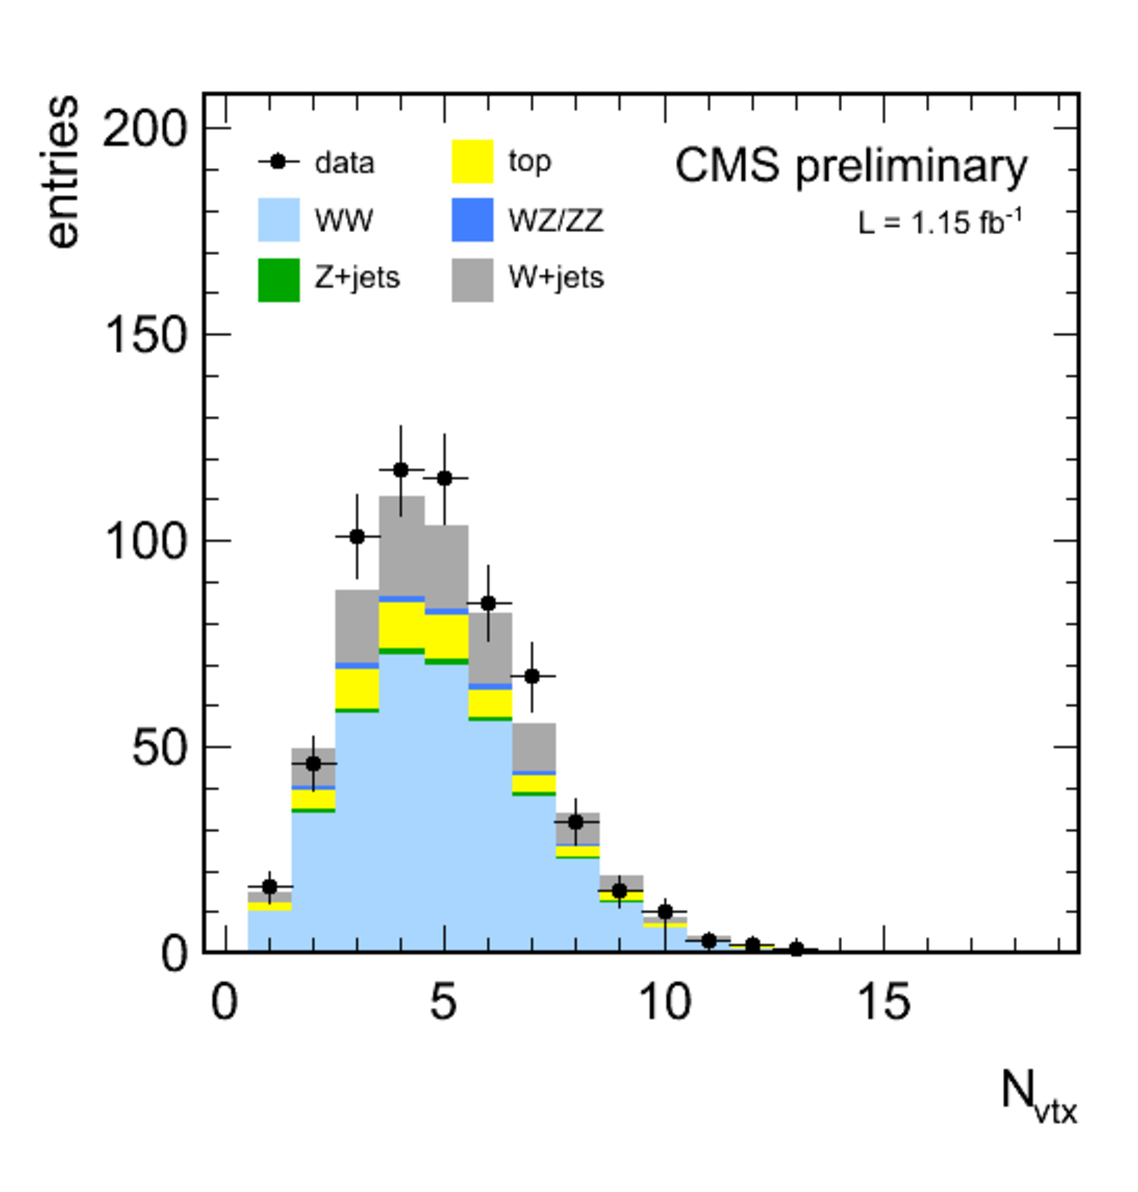
\includegraphics[width=.32\textwidth]{lp_figures/puReweight/histo_nvtx_ww0j_allhwwcuts_EPS.pdf}}
\subfigure[]{
\centering
\label{subfig:lp_pureweight_posteps}
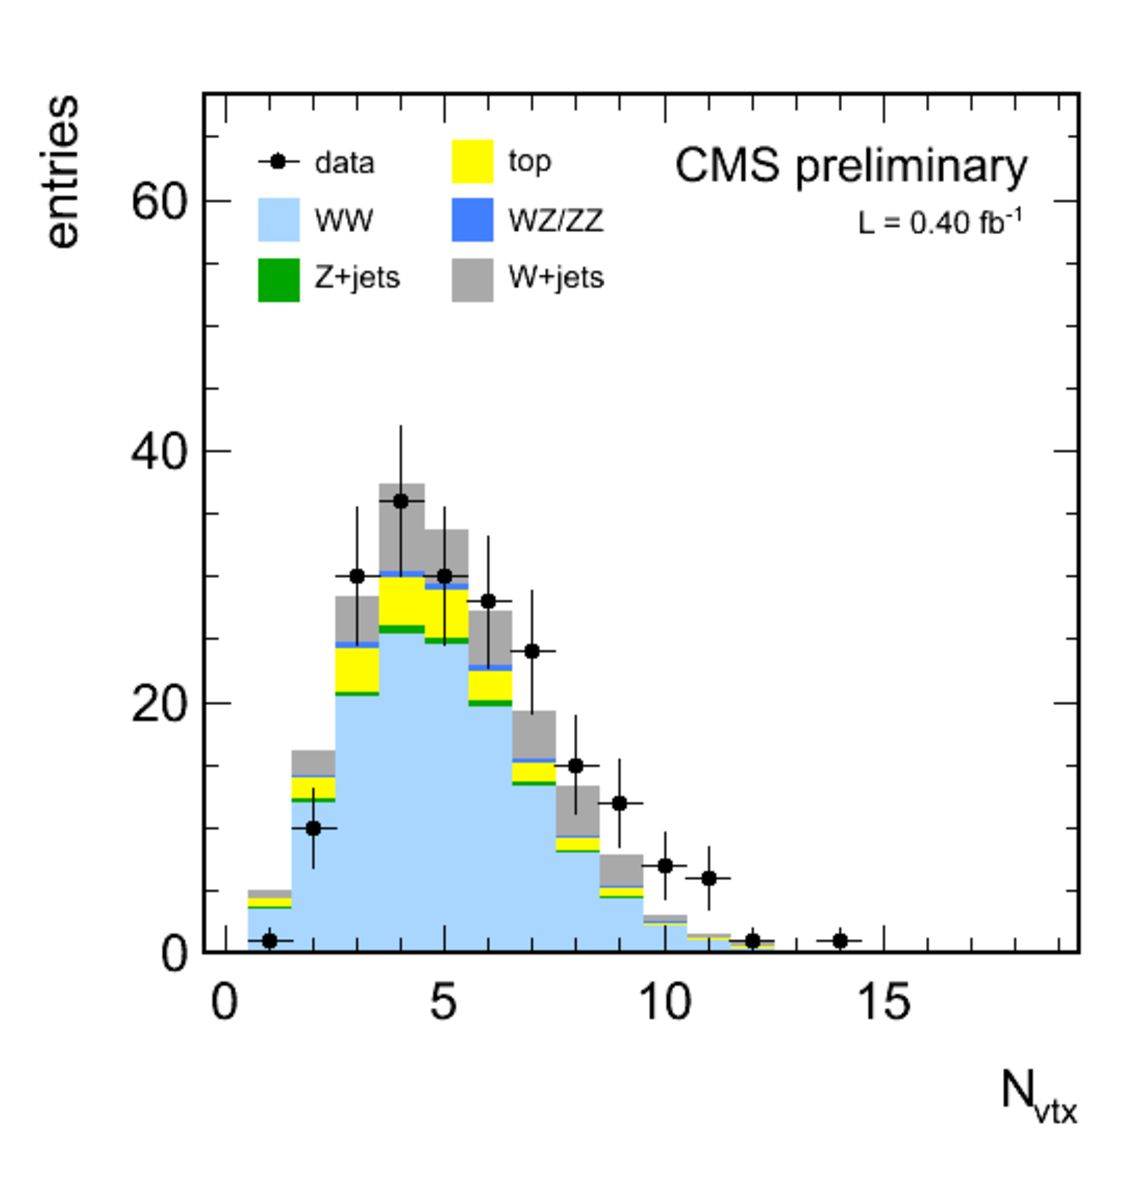
\includegraphics[width=.32\textwidth]{lp_figures/puReweight/histo_nvtx_ww0j_allhwwcuts_POSTEPS.pdf}}
\subfigure[]{
\centering
\label{subfig:lp_pureweight_lp}
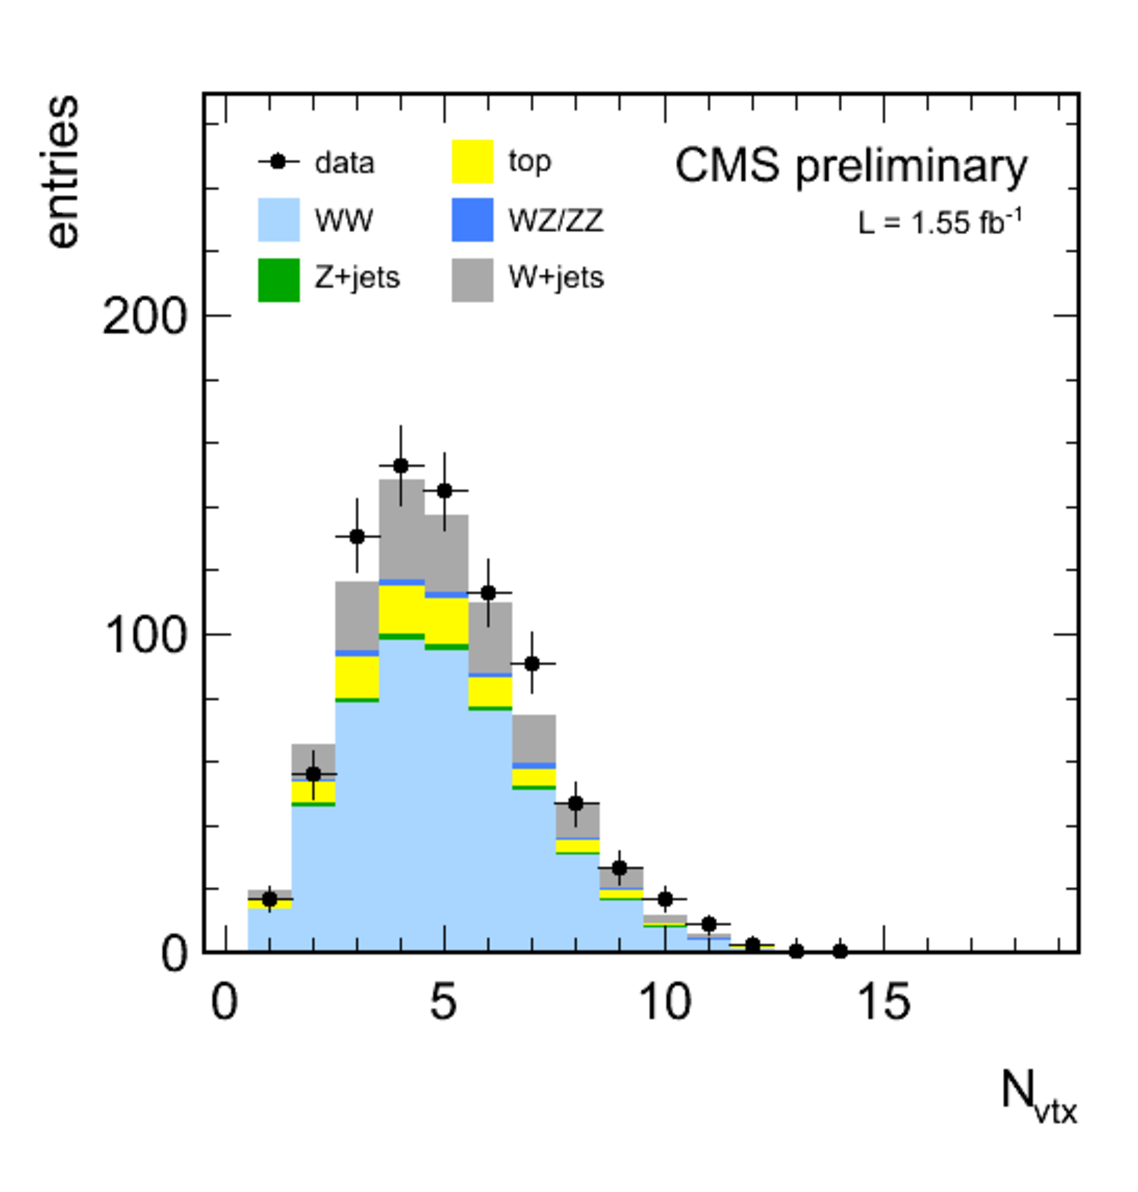
\includegraphics[width=.32\textwidth]{lp_figures/puReweight/histo_nvtx_ww0j_allhwwcuts.pdf}}
\caption{The number of reconstructed vertices in data and simulation
at the WW preselection level after pile-up reweighting
according to the expected pile-up multiplicity
\subref{subfig:lp_pureweight_eps} in the EPS dataset;
\subref{subfig:lp_pureweight_posteps} in the post-EPS dataset;
\subref{subfig:lp_pureweight_lp} in the LP dataset;
}
\label{fig:lp_ww0j_dilep}
\end{figure}





%===================================================================================================
% Background Estimation tables
\section{Background Estimation}
\label{app:lp_bkgestim}
This is a background Estimation for 1.545$\fb$


\section{Data Validation Plots}
\label{app:lp_postEPSdist}
Plots are normalized to 1$/fb$. 
Error bars are the sum in quadrature of the statistical uncertainty of EPS and post-EPS data. 
EPS dataset corresponds to run$<$170826, post-EPS to run$\geq$170826.

\clearpage

\begin{figure}[!hbtp]
\centering
\subfigure[]{
\centering
\label{subfig:lp_dPhi_ww0j}
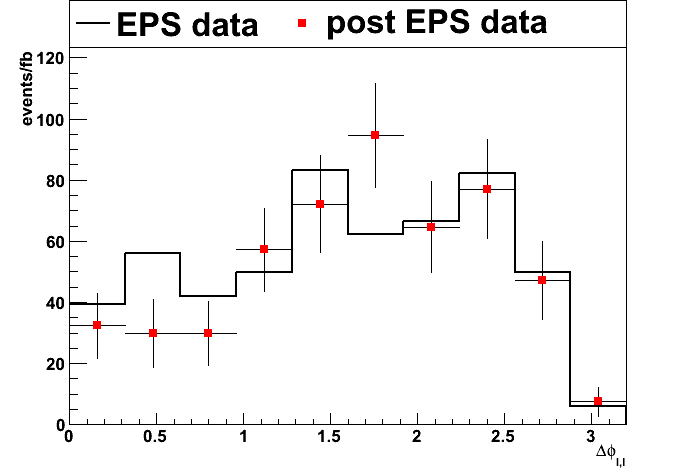
\includegraphics[width=.32\textwidth]{lp_figures/postEPSvalid/hm0/dPhi_ww0j.png}}
\subfigure[]{
\centering
\label{subfig:lp_dilepmass_ww0j}
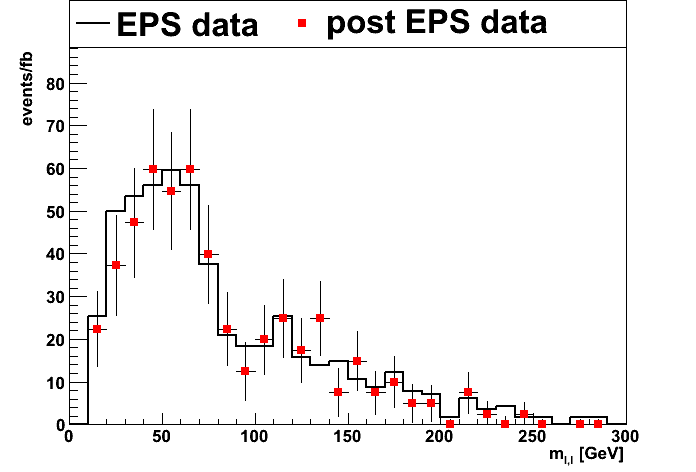
\includegraphics[width=.32\textwidth]{lp_figures/postEPSvalid/hm0/dilepmass_ww0j.png}}\\
\subfigure[]{
\centering
\label{subfig:lp_dileppt_ww0j}
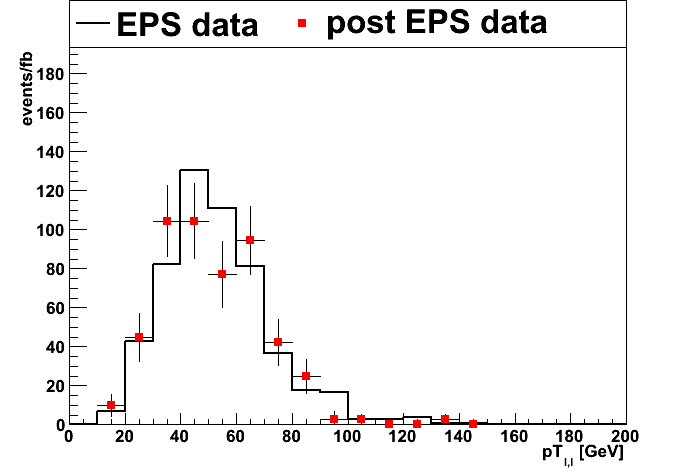
\includegraphics[width=.32\textwidth]{lp_figures/postEPSvalid/hm0/dileppt_ww0j.png}}
\subfigure[]{
\centering
\label{subfig:lp_type_ww0j}
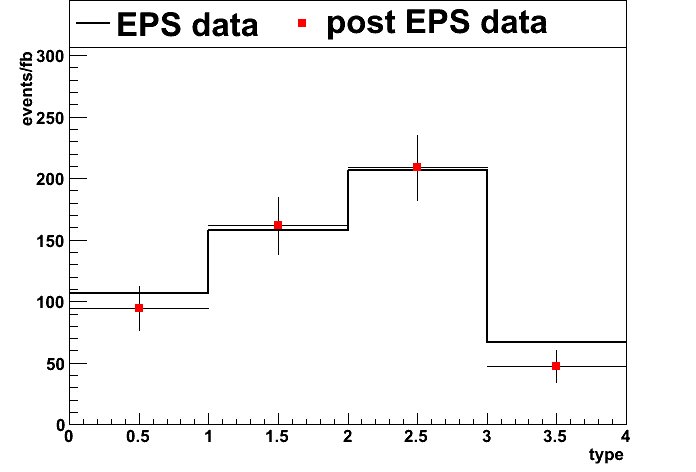
\includegraphics[width=.32\textwidth]{lp_figures/postEPSvalid/hm0/type_ww0j.png}}
\caption{EPS and post-EPS data comparison: 0-jet bin, all final states. 
\subref{subfig:lp_dPhi_ww0j} $\Delta\phi$ between the two leptons;
\subref{subfig:lp_dilepmass_ww0j} di-lepton invariant mass;
\subref{subfig:lp_dileppt_ww0j} di-lepton transverse momentum;
\subref{subfig:lp_type_ww0j} di-lepton type ($\mu\mu$=0, $\mu e$=2, $e\mu$=2, $ee$=3).
}
\label{fig:lp_ww0j_dilep}
\end{figure}

\begin{figure}[!hbtp]
\centering
\subfigure[]{
\centering
\label{subfig:lp_lep1pt_ww0j}
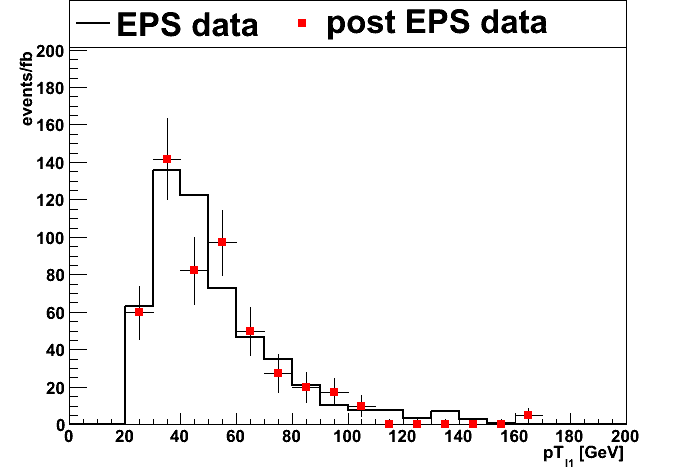
\includegraphics[width=.32\textwidth]{lp_figures/postEPSvalid/hm0/lep1pt_ww0j.png}}
\subfigure[]{
\centering
\label{subfig:lp_lep2pt_ww0j}
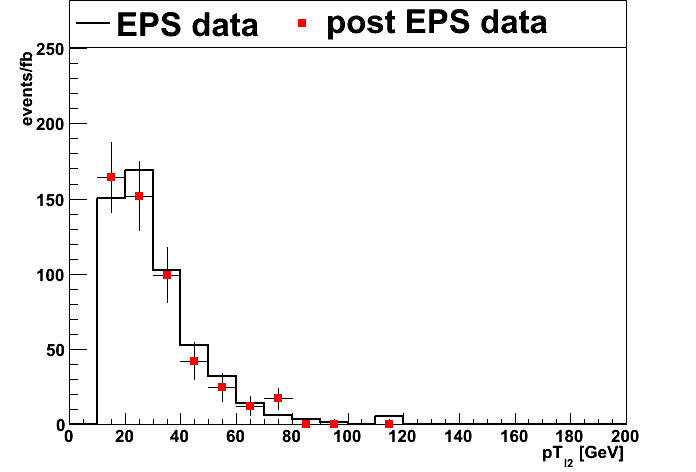
\includegraphics[width=.32\textwidth]{lp_figures/postEPSvalid/hm0/lep2pt_ww0j.png}}
\subfigure[]{
\centering
\label{subfig:lp_jet1pt_ww0j}
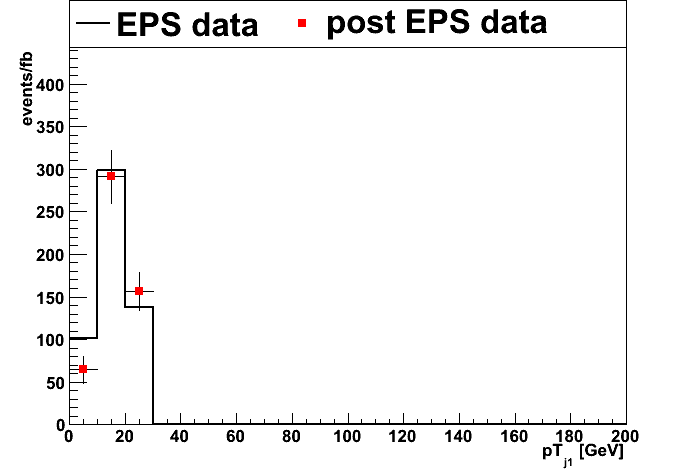
\includegraphics[width=.32\textwidth]{lp_figures/postEPSvalid/hm0/jet1pt_ww0j.png}}\\
\subfigure[]{
\centering
\label{subfig:lp_pmet_ww0j}
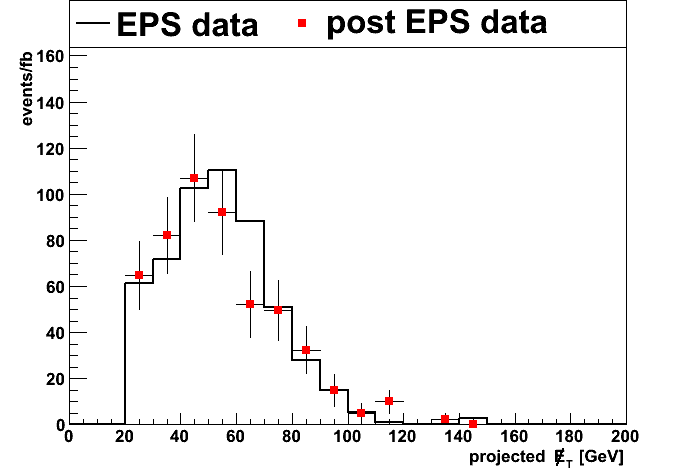
\includegraphics[width=.32\textwidth]{lp_figures/postEPSvalid/hm0/pmet_ww0j.png}}
\subfigure[]{
\centering
\label{subfig:lp_pTrackMet_ww0j}
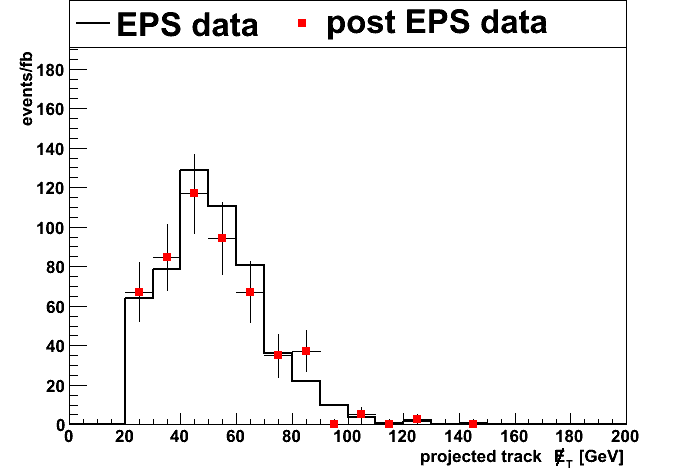
\includegraphics[width=.32\textwidth]{lp_figures/postEPSvalid/hm0/pTrackMet_ww0j.png}}
\subfigure[]{
\centering
\label{subfig:lp_mt_ww0j}
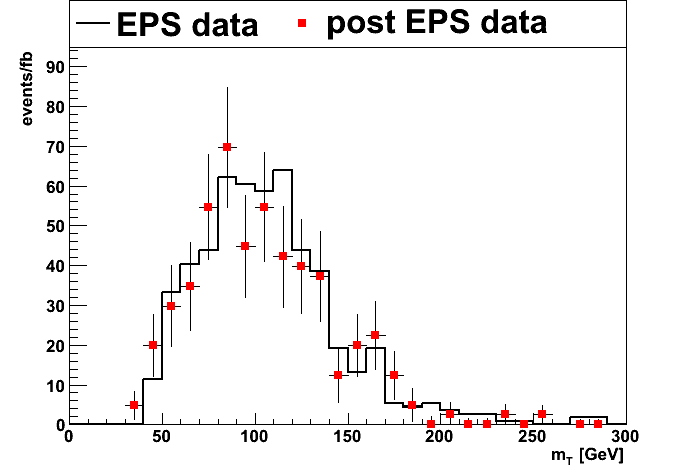
\includegraphics[width=.32\textwidth]{lp_figures/postEPSvalid/hm0/mt_ww0j.png}}
\caption{EPS and post-EPS data comparison: 0-jet bin, all final states. 
\subref{subfig:lp_lep1pt_ww0j} leading lepton $p_T$;
\subref{subfig:lp_lep2pt_ww0j} trailing lepton $p_T$;
\subref{subfig:lp_jet1pt_ww0j} leading jet $p_T$;
\subref{subfig:lp_pmet_ww0j} projected MET;
\subref{subfig:lp_pTrackMet_ww0j} projected track-MET;
\subref{subfig:lp_mt_ww0j} transverse mass of dilepton-MET system.
}
\label{fig:lp_ww0j_lepjetmet}
\end{figure}

\clearpage

\begin{figure}[!hbtp]
\centering
\subfigure[]{
\centering
\label{subfig:lp_dPhi_ww0jmm}
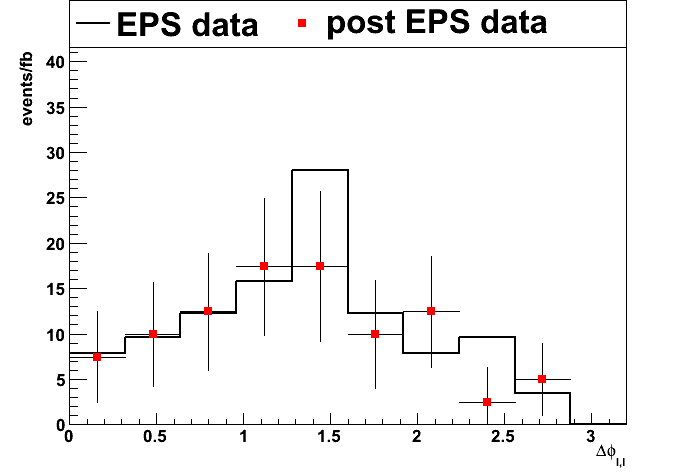
\includegraphics[width=.32\textwidth]{lp_figures/postEPSvalid/hm0/dPhi_ww0jmm.png}}
\subfigure[]{
\centering
\label{subfig:lp_dilepmass_ww0jmm}
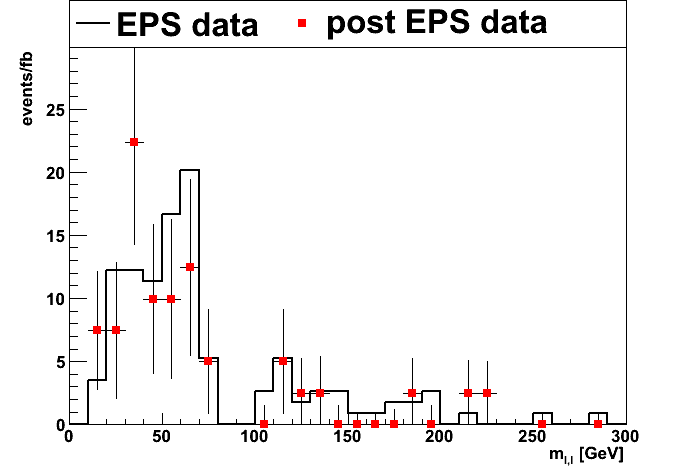
\includegraphics[width=.32\textwidth]{lp_figures/postEPSvalid/hm0/dilepmass_ww0jmm.png}}\\
\subfigure[]{
\centering
\label{subfig:lp_dileppt_ww0jmm}
\includegraphics[width=.32\textwidth]{lp_figures/postEPSvalid/hm0/dileppt_ww0jmm.png}}
\subfigure[]{
\centering
\label{subfig:lp_type_ww0jmm}
\includegraphics[width=.32\textwidth]{lp_figures/postEPSvalid/hm0/type_ww0jmm.png}}
\caption{EPS and post-EPS data comparison: 0-jet bin, $\mu\mu$ final state. 
\subref{subfig:lp_dPhi_ww0jmm} $\Delta\phi$ between the two leptons;
\subref{subfig:lp_dilepmass_ww0jmm} di-lepton invariant mass;
\subref{subfig:lp_dileppt_ww0jmm} di-lepton transverse momentum;
\subref{subfig:lp_type_ww0jmm} di-lepton type ($\mu\mu$=0, $\mu e$=2, $e\mu$=2, $ee$=3).
}
\label{fig:lp_ww0jmm_dilep}
\end{figure}

\begin{figure}[!hbtp]
\centering
\subfigure[]{
\centering
\label{subfig:lp_lep1pt_ww0jmm}
\includegraphics[width=.32\textwidth]{lp_figures/postEPSvalid/hm0/lep1pt_ww0jmm.png}}
\subfigure[]{
\centering
\label{subfig:lp_lep2pt_ww0jmm}
\includegraphics[width=.32\textwidth]{lp_figures/postEPSvalid/hm0/lep2pt_ww0jmm.png}}
\subfigure[]{
\centering
\label{subfig:lp_jet1pt_ww0jmm}
\includegraphics[width=.32\textwidth]{lp_figures/postEPSvalid/hm0/jet1pt_ww0jmm.png}}\\
\subfigure[]{
\centering
\label{subfig:lp_pmet_ww0jmm}
\includegraphics[width=.32\textwidth]{lp_figures/postEPSvalid/hm0/pmet_ww0jmm.png}}
\subfigure[]{
\centering
\label{subfig:lp_pTrackMet_ww0jmm}
\includegraphics[width=.32\textwidth]{lp_figures/postEPSvalid/hm0/pTrackMet_ww0jmm.png}}
\subfigure[]{
\centering
\label{subfig:lp_mt_ww0jmm}
\includegraphics[width=.32\textwidth]{lp_figures/postEPSvalid/hm0/mt_ww0jmm.png}}
\caption{EPS and post-EPS data comparison: 0-jet bin, $\mu\mu$ final state. 
\subref{subfig:lp_lep1pt_ww0jmm} leading lepton $p_T$;
\subref{subfig:lp_lep2pt_ww0jmm} trailing lepton $p_T$;
\subref{subfig:lp_jet1pt_ww0jmm} leading jet $p_T$;
\subref{subfig:lp_pmet_ww0jmm} projected MET;
\subref{subfig:lp_pTrackMet_ww0jmm} projected track-MET;
\subref{subfig:lp_mt_ww0jmm} transverse mass of dilepton-MET system.
}
\label{fig:lp_ww0jmm_lepjetmet}
\end{figure}

\clearpage

\begin{figure}[!hbtp]
\centering
\subfigure[]{
\centering
\label{subfig:lp_dPhi_ww1j}
\includegraphics[width=.32\textwidth]{lp_figures/postEPSvalid/hm0/dPhi_ww1j.png}}
\subfigure[]{
\centering
\label{subfig:lp_dilepmass_ww1j}
\includegraphics[width=.32\textwidth]{lp_figures/postEPSvalid/hm0/dilepmass_ww1j.png}}\\
\subfigure[]{
\centering
\label{subfig:lp_dileppt_ww1j}
\includegraphics[width=.32\textwidth]{lp_figures/postEPSvalid/hm0/dileppt_ww1j.png}}
\subfigure[]{
\centering
\label{subfig:lp_type_ww1j}
\includegraphics[width=.32\textwidth]{lp_figures/postEPSvalid/hm0/type_ww1j.png}}
\caption{EPS and post-EPS data comparison: 1-jet bin, all final states. 
\subref{subfig:lp_dPhi_ww1j} $\Delta\phi$ between the two leptons;
\subref{subfig:lp_dilepmass_ww1j} di-lepton invariant mass;
\subref{subfig:lp_dileppt_ww1j} di-lepton transverse momentum;
\subref{subfig:lp_type_ww1j} di-lepton type ($\mu\mu$=0, $\mu e$=2, $e\mu$=2, $ee$=3).
}
\label{fig:lp_ww1j_dilep}
\end{figure}

\begin{figure}[!hbtp]
\centering
\subfigure[]{
\centering
\label{subfig:lp_lep1pt_ww1j}
\includegraphics[width=.32\textwidth]{lp_figures/postEPSvalid/hm0/lep1pt_ww1j.png}}
\subfigure[]{
\centering
\label{subfig:lp_lep2pt_ww1j}
\includegraphics[width=.32\textwidth]{lp_figures/postEPSvalid/hm0/lep2pt_ww1j.png}}
\subfigure[]{
\centering
\label{subfig:lp_jet1pt_ww1j}
\includegraphics[width=.32\textwidth]{lp_figures/postEPSvalid/hm0/jet1pt_ww1j.png}}\\
\subfigure[]{
\centering
\label{subfig:lp_pmet_ww1j}
\includegraphics[width=.32\textwidth]{lp_figures/postEPSvalid/hm0/pmet_ww1j.png}}
\subfigure[]{
\centering
\label{subfig:lp_pTrackMet_ww1j}
\includegraphics[width=.32\textwidth]{lp_figures/postEPSvalid/hm0/pTrackMet_ww1j.png}}
\subfigure[]{
\centering
\label{subfig:lp_mt_ww1j}
\includegraphics[width=.32\textwidth]{lp_figures/postEPSvalid/hm0/mt_ww1j.png}}
\caption{EPS and post-EPS data comparison: 1-jet bin, all final states. 
\subref{subfig:lp_lep1pt_ww1j} leading lepton $p_T$;
\subref{subfig:lp_lep2pt_ww1j} trailing lepton $p_T$;
\subref{subfig:lp_jet1pt_ww1j} leading jet $p_T$;
\subref{subfig:lp_pmet_ww1j} projected MET;
\subref{subfig:lp_pTrackMet_ww1j} projected track-MET;
\subref{subfig:lp_mt_ww1j} transverse mass of dilepton-MET system.
}
\label{fig:lp_ww1j_lepjetmet}
\end{figure}

\clearpage

\begin{figure}[!hbtp]
\centering
\subfigure[]{
\centering
\label{subfig:lp_dPhi_ww2j}
\includegraphics[width=.32\textwidth]{lp_figures/postEPSvalid/hm0/dPhi_ww2j.png}}
\subfigure[]{
\centering
\label{subfig:lp_dilepmass_ww2j}
\includegraphics[width=.32\textwidth]{lp_figures/postEPSvalid/hm0/dilepmass_ww2j.png}}\\
\subfigure[]{
\centering
\label{subfig:lp_dileppt_ww2j}
\includegraphics[width=.32\textwidth]{lp_figures/postEPSvalid/hm0/dileppt_ww2j.png}}
\subfigure[]{
\centering
\label{subfig:lp_type_ww2j}
\includegraphics[width=.32\textwidth]{lp_figures/postEPSvalid/hm0/type_ww2j.png}}
\caption{EPS and post-EPS data comparison: 2-jet bin, all final states. 
\subref{subfig:lp_dPhi_ww2j} $\Delta\phi$ between the two leptons;
\subref{subfig:lp_dilepmass_ww2j} di-lepton invariant mass;
\subref{subfig:lp_dileppt_ww2j} di-lepton transverse momentum;
\subref{subfig:lp_type_ww2j} di-lepton type ($\mu\mu$=0, $\mu e$=2, $e\mu$=2, $ee$=3).
}
\label{fig:lp_ww2j_dilep}
\end{figure}

\begin{figure}[!hbtp]
\centering
\subfigure[]{
\centering
\label{subfig:lp_lep1pt_ww2j}
\includegraphics[width=.32\textwidth]{lp_figures/postEPSvalid/hm0/lep1pt_ww2j.png}}
\subfigure[]{
\centering
\label{subfig:lp_lep2pt_ww2j}
\includegraphics[width=.32\textwidth]{lp_figures/postEPSvalid/hm0/lep2pt_ww2j.png}}
\subfigure[]{
\centering
\label{subfig:lp_jet1pt_ww2j}
\includegraphics[width=.32\textwidth]{lp_figures/postEPSvalid/hm0/jet1pt_ww2j.png}}\\
\subfigure[]{
\centering
\label{subfig:lp_pmet_ww2j}
\includegraphics[width=.32\textwidth]{lp_figures/postEPSvalid/hm0/pmet_ww2j.png}}
\subfigure[]{
\centering
\label{subfig:lp_pTrackMet_ww2j}
\includegraphics[width=.32\textwidth]{lp_figures/postEPSvalid/hm0/pTrackMet_ww2j.png}}
\subfigure[]{
\centering
\label{subfig:lp_mt_ww2j}
\includegraphics[width=.32\textwidth]{lp_figures/postEPSvalid/hm0/mt_ww2j.png}}
\caption{EPS and post-EPS data comparison: 2-jet bin, all final states. 
\subref{subfig:lp_lep1pt_ww2j} leading lepton $p_T$;
\subref{subfig:lp_lep2pt_ww2j} trailing lepton $p_T$;
\subref{subfig:lp_jet1pt_ww2j} leading jet $p_T$;
\subref{subfig:lp_pmet_ww2j} projected MET;
\subref{subfig:lp_pTrackMet_ww2j} projected track-MET;
\subref{subfig:lp_mt_ww2j} transverse mass of dilepton-MET system.
}
\label{fig:lp_ww2j_lepjetmet}
\end{figure}

\clearpage


%%      \subsection{Background Estimation for \lpintlumi}
%%     \label{app:lp_bkgestim}
%%      This is a background Estimation for 1.545$\fb$


%%      \subsection{Final limits for \lpintlumi}
%%     \label{app:lp_limits}
%%      This is a final limit



%%     \subsection{MVA output plots}
%%     \label{app:lp_mvaplots}
%%     \subsubsection{EPS distributions}

This section contains the MVA output plots for the EPS dataset for $m_H$=115, 120, 130, 140, 150, 160, 200 GeV analyses split in opposte and same flavor, 
0-jet and 1-jet bin (Figures~\ref{fig:lp_mva_115_EPS}-\ref{fig:lp_mva_200_EPS}).

\begin{figure}[!hbtp]
\centering
\subfigure[]{
\centering
\label{subfig:lp_mva_115_0j_of_EPS}
\includegraphics[width=.40\textwidth]{lp_figures/histo_mva_115_0j_of_EPS.png}}
\subfigure[]{
\centering
\label{subfig:lp_mva_115_0j_sf_EPS}
\includegraphics[width=.40\textwidth]{lp_figures/histo_mva_115_0j_sf_EPS.png}}\\
\subfigure[]{
\centering
\label{subfig:lp_mva_115_1j_of_EPS}
\includegraphics[width=.40\textwidth]{lp_figures/histo_mva_115_1j_of_EPS.png}}
\subfigure[]{
\centering
\label{subfig:lp_mva_115_1j_sf_EPS}
\includegraphics[width=.40\textwidth]{lp_figures/histo_mva_115_1j_sf_EPS.png}}
\caption{
MVA output for $m_H$=115 GeV EPS analysis: 
0-jet OF \subref{subfig:lp_mva_115_0j_of_EPS},
0-jet SF \subref{subfig:lp_mva_115_0j_sf_EPS},
1-jet OF \subref{subfig:lp_mva_115_1j_of_EPS},
1-jet SF \subref{subfig:lp_mva_115_1j_sf_EPS}
.}
\label{fig:lp_mva_115_EPS}
\end{figure}

\begin{figure}[!hbtp]
\centering
\subfigure[]{
\centering
\label{subfig:lp_mva_120_0j_of_EPS}
\includegraphics[width=.40\textwidth]{lp_figures/histo_mva_120_0j_of_EPS.png}}
\subfigure[]{
\centering
\label{subfig:lp_mva_120_0j_sf_EPS}
\includegraphics[width=.40\textwidth]{lp_figures/histo_mva_120_0j_sf_EPS.png}}\\
\subfigure[]{
\centering
\label{subfig:lp_mva_120_1j_of_EPS}
\includegraphics[width=.40\textwidth]{lp_figures/histo_mva_120_1j_of_EPS.png}}
\subfigure[]{
\centering
\label{subfig:lp_mva_120_1j_sf_EPS}
\includegraphics[width=.40\textwidth]{lp_figures/histo_mva_120_1j_sf_EPS.png}}
\caption{
MVA output for $m_H$=120 GeV EPS analysis: 
0-jet OF \subref{subfig:lp_mva_120_0j_of_EPS},
0-jet SF \subref{subfig:lp_mva_120_0j_sf_EPS},
1-jet OF \subref{subfig:lp_mva_120_1j_of_EPS},
1-jet SF \subref{subfig:lp_mva_120_1j_sf_EPS}
.}
\label{fig:lp_mva_120_EPS}
\end{figure}

\begin{figure}[!hbtp]
\centering
\subfigure[]{
\centering
\label{subfig:lp_mva_130_0j_of_EPS}
\includegraphics[width=.40\textwidth]{lp_figures/histo_mva_130_0j_of_EPS.png}}
\subfigure[]{
\centering
\label{subfig:lp_mva_130_0j_sf_EPS}
\includegraphics[width=.40\textwidth]{lp_figures/histo_mva_130_0j_sf_EPS.png}}\\
\subfigure[]{
\centering
\label{subfig:lp_mva_130_1j_of_EPS}
\includegraphics[width=.40\textwidth]{lp_figures/histo_mva_130_1j_of_EPS.png}}
\subfigure[]{
\centering
\label{subfig:lp_mva_130_1j_sf_EPS}
\includegraphics[width=.40\textwidth]{lp_figures/histo_mva_130_1j_sf_EPS.png}}
\caption{
MVA output for $m_H$=130 GeV EPS analysis: 
0-jet OF \subref{subfig:lp_mva_130_0j_of_EPS},
0-jet SF \subref{subfig:lp_mva_130_0j_sf_EPS},
1-jet OF \subref{subfig:lp_mva_130_1j_of_EPS},
1-jet SF \subref{subfig:lp_mva_130_1j_sf_EPS}
.}
\label{fig:lp_mva_130_EPS}
\end{figure}

\begin{figure}[!hbtp]
\centering
\subfigure[]{
\centering
\label{subfig:lp_mva_140_0j_of_EPS}
\includegraphics[width=.40\textwidth]{lp_figures/histo_mva_140_0j_of_EPS.png}}
\subfigure[]{
\centering
\label{subfig:lp_mva_140_0j_sf_EPS}
\includegraphics[width=.40\textwidth]{lp_figures/histo_mva_140_0j_sf_EPS.png}}\\
\subfigure[]{
\centering
\label{subfig:lp_mva_140_1j_of_EPS}
\includegraphics[width=.40\textwidth]{lp_figures/histo_mva_140_1j_of_EPS.png}}
\subfigure[]{
\centering
\label{subfig:lp_mva_140_1j_sf_EPS}
\includegraphics[width=.40\textwidth]{lp_figures/histo_mva_140_1j_sf_EPS.png}}
\caption{
MVA output for $m_H$=140 GeV EPS analysis: 
0-jet OF \subref{subfig:lp_mva_140_0j_of_EPS},
0-jet SF \subref{subfig:lp_mva_140_0j_sf_EPS},
1-jet OF \subref{subfig:lp_mva_140_1j_of_EPS},
1-jet SF \subref{subfig:lp_mva_140_1j_sf_EPS}
.}
\label{fig:lp_mva_140_EPS}
\end{figure}

\begin{figure}[!hbtp]
\centering
\subfigure[]{
\centering
\label{subfig:lp_mva_150_0j_of_EPS}
\includegraphics[width=.40\textwidth]{lp_figures/histo_mva_150_0j_of_EPS.png}}
\subfigure[]{
\centering
\label{subfig:lp_mva_150_0j_sf_EPS}
\includegraphics[width=.40\textwidth]{lp_figures/histo_mva_150_0j_sf_EPS.png}}\\
\subfigure[]{
\centering
\label{subfig:lp_mva_150_1j_of_EPS}
\includegraphics[width=.40\textwidth]{lp_figures/histo_mva_150_1j_of_EPS.png}}
\subfigure[]{
\centering
\label{subfig:lp_mva_150_1j_sf_EPS}
\includegraphics[width=.40\textwidth]{lp_figures/histo_mva_150_1j_sf_EPS.png}}
\caption{
MVA output for $m_H$=150 GeV EPS analysis: 
0-jet OF \subref{subfig:lp_mva_150_0j_of_EPS},
0-jet SF \subref{subfig:lp_mva_150_0j_sf_EPS},
1-jet OF \subref{subfig:lp_mva_150_1j_of_EPS},
1-jet SF \subref{subfig:lp_mva_150_1j_sf_EPS}
.}
\label{fig:lp_mva_150_EPS}
\end{figure}

\begin{figure}[!hbtp]
\centering
\subfigure[]{
\centering
\label{subfig:lp_mva_160_0j_of_EPS}
\includegraphics[width=.40\textwidth]{lp_figures/histo_mva_160_0j_of_EPS.png}}
\subfigure[]{
\centering
\label{subfig:lp_mva_160_0j_sf_EPS}
\includegraphics[width=.40\textwidth]{lp_figures/histo_mva_160_0j_sf_EPS.png}}\\
\subfigure[]{
\centering
\label{subfig:lp_mva_160_1j_of_EPS}
\includegraphics[width=.40\textwidth]{lp_figures/histo_mva_160_1j_of_EPS.png}}
\subfigure[]{
\centering
\label{subfig:lp_mva_160_1j_sf_EPS}
\includegraphics[width=.40\textwidth]{lp_figures/histo_mva_160_1j_sf_EPS.png}}
\caption{
MVA output for $m_H$=160 GeV EPS analysis: 
0-jet OF \subref{subfig:lp_mva_160_0j_of_EPS},
0-jet SF \subref{subfig:lp_mva_160_0j_sf_EPS},
1-jet OF \subref{subfig:lp_mva_160_1j_of_EPS},
1-jet SF \subref{subfig:lp_mva_160_1j_sf_EPS}
.}
\label{fig:lp_mva_160_EPS}
\end{figure}

\begin{figure}[!hbtp]
\centering
\subfigure[]{
\centering
\label{subfig:lp_mva_200_0j_of_EPS}
\includegraphics[width=.40\textwidth]{lp_figures/histo_mva_200_0j_of_EPS.png}}
\subfigure[]{
\centering
\label{subfig:lp_mva_200_0j_sf_EPS}
\includegraphics[width=.40\textwidth]{lp_figures/histo_mva_200_0j_sf_EPS.png}}\\
\subfigure[]{
\centering
\label{subfig:lp_mva_200_1j_of_EPS}
\includegraphics[width=.40\textwidth]{lp_figures/histo_mva_200_1j_of_EPS.png}}
\subfigure[]{
\centering
\label{subfig:lp_mva_200_1j_sf_EPS}
\includegraphics[width=.40\textwidth]{lp_figures/histo_mva_200_1j_sf_EPS.png}}
\caption{
MVA output for $m_H$=200 GeV EPS analysis: 
0-jet OF \subref{subfig:lp_mva_200_0j_of_EPS},
0-jet SF \subref{subfig:lp_mva_200_0j_sf_EPS},
1-jet OF \subref{subfig:lp_mva_200_1j_of_EPS},
1-jet SF \subref{subfig:lp_mva_200_1j_sf_EPS}
.}
\label{fig:lp_mva_200_EPS}
\end{figure}

\clearpage

%%     \subsection{Post-EPS distributions}

This section contains the MVA output plots for the post-EPS dataset for $m_H$=115, 120, 130, 140, 150, 160, 200 GeV analyses split in opposte and same flavor, 
0-jet and 1-jet bin (Figures~\ref{fig:lp_mva_115_POSTEPS}-\ref{fig:lp_mva_200_POSTEPS}).

\begin{figure}[!hbtp]
\centering
\subfigure[]{
\centering
\label{subfig:lp_mva_115_0j_of_POSTEPS}
\includegraphics[width=.40\textwidth]{lp_figures/histo_mva_115_0j_of_POSTEPS.png}}
\subfigure[]{
\centering
\label{subfig:lp_mva_115_0j_sf_POSTEPS}
\includegraphics[width=.40\textwidth]{lp_figures/histo_mva_115_0j_sf_POSTEPS.png}}\\
\subfigure[]{
\centering
\label{subfig:lp_mva_115_1j_of_POSTEPS}
\includegraphics[width=.40\textwidth]{lp_figures/histo_mva_115_1j_of_POSTEPS.png}}
\subfigure[]{
\centering
\label{subfig:lp_mva_115_1j_sf_POSTEPS}
\includegraphics[width=.40\textwidth]{lp_figures/histo_mva_115_1j_sf_POSTEPS.png}}
\caption{
MVA output for $m_H$=115 GeV post-EPS analysis: 
0-jet OF \subref{subfig:lp_mva_115_0j_of_POSTEPS},
0-jet SF \subref{subfig:lp_mva_115_0j_sf_POSTEPS},
1-jet OF \subref{subfig:lp_mva_115_1j_of_POSTEPS},
1-jet SF \subref{subfig:lp_mva_115_1j_sf_POSTEPS}
.}
\label{fig:lp_mva_115_POSTEPS}
\end{figure}

\begin{figure}[!hbtp]
\centering
\subfigure[]{
\centering
\label{subfig:lp_mva_120_0j_of_POSTEPS}
\includegraphics[width=.40\textwidth]{lp_figures/histo_mva_120_0j_of_POSTEPS.png}}
\subfigure[]{
\centering
\label{subfig:lp_mva_120_0j_sf_POSTEPS}
\includegraphics[width=.40\textwidth]{lp_figures/histo_mva_120_0j_sf_POSTEPS.png}}\\
\subfigure[]{
\centering
\label{subfig:lp_mva_120_1j_of_POSTEPS}
\includegraphics[width=.40\textwidth]{lp_figures/histo_mva_120_1j_of_POSTEPS.png}}
\subfigure[]{
\centering
\label{subfig:lp_mva_120_1j_sf_POSTEPS}
\includegraphics[width=.40\textwidth]{lp_figures/histo_mva_120_1j_sf_POSTEPS.png}}
\caption{
MVA output for $m_H$=120 GeV post-EPS analysis: 
0-jet OF \subref{subfig:lp_mva_120_0j_of_POSTEPS},
0-jet SF \subref{subfig:lp_mva_120_0j_sf_POSTEPS},
1-jet OF \subref{subfig:lp_mva_120_1j_of_POSTEPS},
1-jet SF \subref{subfig:lp_mva_120_1j_sf_POSTEPS}
.}
\label{fig:lp_mva_120_POSTEPS}
\end{figure}

\begin{figure}[!hbtp]
\centering
\subfigure[]{
\centering
\label{subfig:lp_mva_130_0j_of_POSTEPS}
\includegraphics[width=.40\textwidth]{lp_figures/histo_mva_130_0j_of_POSTEPS.png}}
\subfigure[]{
\centering
\label{subfig:lp_mva_130_0j_sf_POSTEPS}
\includegraphics[width=.40\textwidth]{lp_figures/histo_mva_130_0j_sf_POSTEPS.png}}\\
\subfigure[]{
\centering
\label{subfig:lp_mva_130_1j_of_POSTEPS}
\includegraphics[width=.40\textwidth]{lp_figures/histo_mva_130_1j_of_POSTEPS.png}}
\subfigure[]{
\centering
\label{subfig:lp_mva_130_1j_sf_POSTEPS}
\includegraphics[width=.40\textwidth]{lp_figures/histo_mva_130_1j_sf_POSTEPS.png}}
\caption{
MVA output for $m_H$=130 GeV post-EPS analysis: 
0-jet OF \subref{subfig:lp_mva_130_0j_of_POSTEPS},
0-jet SF \subref{subfig:lp_mva_130_0j_sf_POSTEPS},
1-jet OF \subref{subfig:lp_mva_130_1j_of_POSTEPS},
1-jet SF \subref{subfig:lp_mva_130_1j_sf_POSTEPS}
.}
\label{fig:lp_mva_130_POSTEPS}
\end{figure}

\begin{figure}[!hbtp]
\centering
\subfigure[]{
\centering
\label{subfig:lp_mva_140_0j_of_POSTEPS}
\includegraphics[width=.40\textwidth]{lp_figures/histo_mva_140_0j_of_POSTEPS.png}}
\subfigure[]{
\centering
\label{subfig:lp_mva_140_0j_sf_POSTEPS}
\includegraphics[width=.40\textwidth]{lp_figures/histo_mva_140_0j_sf_POSTEPS.png}}\\
\subfigure[]{
\centering
\label{subfig:lp_mva_140_1j_of_POSTEPS}
\includegraphics[width=.40\textwidth]{lp_figures/histo_mva_140_1j_of_POSTEPS.png}}
\subfigure[]{
\centering
\label{subfig:lp_mva_140_1j_sf_POSTEPS}
\includegraphics[width=.40\textwidth]{lp_figures/histo_mva_140_1j_sf_POSTEPS.png}}
\caption{
MVA output for $m_H$=140 GeV post-EPS analysis: 
0-jet OF \subref{subfig:lp_mva_140_0j_of_POSTEPS},
0-jet SF \subref{subfig:lp_mva_140_0j_sf_POSTEPS},
1-jet OF \subref{subfig:lp_mva_140_1j_of_POSTEPS},
1-jet SF \subref{subfig:lp_mva_140_1j_sf_POSTEPS}
.}
\label{fig:lp_mva_140_POSTEPS}
\end{figure}

\begin{figure}[!hbtp]
\centering
\subfigure[]{
\centering
\label{subfig:lp_mva_150_0j_of_POSTEPS}
\includegraphics[width=.40\textwidth]{lp_figures/histo_mva_150_0j_of_POSTEPS.png}}
\subfigure[]{
\centering
\label{subfig:lp_mva_150_0j_sf_POSTEPS}
\includegraphics[width=.40\textwidth]{lp_figures/histo_mva_150_0j_sf_POSTEPS.png}}\\
\subfigure[]{
\centering
\label{subfig:lp_mva_150_1j_of_POSTEPS}
\includegraphics[width=.40\textwidth]{lp_figures/histo_mva_150_1j_of_POSTEPS.png}}
\subfigure[]{
\centering
\label{subfig:lp_mva_150_1j_sf_POSTEPS}
\includegraphics[width=.40\textwidth]{lp_figures/histo_mva_150_1j_sf_POSTEPS.png}}
\caption{
MVA output for $m_H$=150 GeV post-EPS analysis: 
0-jet OF \subref{subfig:lp_mva_150_0j_of_POSTEPS},
0-jet SF \subref{subfig:lp_mva_150_0j_sf_POSTEPS},
1-jet OF \subref{subfig:lp_mva_150_1j_of_POSTEPS},
1-jet SF \subref{subfig:lp_mva_150_1j_sf_POSTEPS}
.}
\label{fig:lp_mva_150_POSTEPS}
\end{figure}

\begin{figure}[!hbtp]
\centering
\subfigure[]{
\centering
\label{subfig:lp_mva_160_0j_of_POSTEPS}
\includegraphics[width=.40\textwidth]{lp_figures/histo_mva_160_0j_of_POSTEPS.png}}
\subfigure[]{
\centering
\label{subfig:lp_mva_160_0j_sf_POSTEPS}
\includegraphics[width=.40\textwidth]{lp_figures/histo_mva_160_0j_sf_POSTEPS.png}}\\
\subfigure[]{
\centering
\label{subfig:lp_mva_160_1j_of_POSTEPS}
\includegraphics[width=.40\textwidth]{lp_figures/histo_mva_160_1j_of_POSTEPS.png}}
\subfigure[]{
\centering
\label{subfig:lp_mva_160_1j_sf_POSTEPS}
\includegraphics[width=.40\textwidth]{lp_figures/histo_mva_160_1j_sf_POSTEPS.png}}
\caption{
MVA output for $m_H$=160 GeV post-EPS analysis: 
0-jet OF \subref{subfig:lp_mva_160_0j_of_POSTEPS},
0-jet SF \subref{subfig:lp_mva_160_0j_sf_POSTEPS},
1-jet OF \subref{subfig:lp_mva_160_1j_of_POSTEPS},
1-jet SF \subref{subfig:lp_mva_160_1j_sf_POSTEPS}
.}
\label{fig:lp_mva_160_POSTEPS}
\end{figure}

\begin{figure}[!hbtp]
\centering
\subfigure[]{
\centering
\label{subfig:lp_mva_200_0j_of_POSTEPS}
\includegraphics[width=.40\textwidth]{lp_figures/histo_mva_200_0j_of_POSTEPS.png}}
\subfigure[]{
\centering
\label{subfig:lp_mva_200_0j_sf_POSTEPS}
\includegraphics[width=.40\textwidth]{lp_figures/histo_mva_200_0j_sf_POSTEPS.png}}\\
\subfigure[]{
\centering
\label{subfig:lp_mva_200_1j_of_POSTEPS}
\includegraphics[width=.40\textwidth]{lp_figures/histo_mva_200_1j_of_POSTEPS.png}}
\subfigure[]{
\centering
\label{subfig:lp_mva_200_1j_sf_POSTEPS}
\includegraphics[width=.40\textwidth]{lp_figures/histo_mva_200_1j_sf_POSTEPS.png}}
\caption{
MVA output for $m_H$=200 GeV post-EPS analysis: 
0-jet OF \subref{subfig:lp_mva_200_0j_of_POSTEPS},
0-jet SF \subref{subfig:lp_mva_200_0j_sf_POSTEPS},
1-jet OF \subref{subfig:lp_mva_200_1j_of_POSTEPS},
1-jet SF \subref{subfig:lp_mva_200_1j_sf_POSTEPS}
.}
\label{fig:lp_mva_200_POSTEPS}
\end{figure}

\clearpage

%%     \subsection{LP distributions}

This section contains the MVA output plots for the LP dataset for $m_H$=115, 120, 130, 140, 150, 160, 200 GeV analyses split in opposte and same flavor, 
0-jet and 1-jet bin (Figures~\ref{fig:lp_mva_115}-\ref{fig:lp_mva_200}).

\begin{figure}[!hbtp]
\centering
\subfigure[]{
\centering
\label{subfig:lp_mva_115_0j_of}
\includegraphics[width=.40\textwidth]{lp_figures/histo_mva_115_0j_of.png}}
\subfigure[]{
\centering
\label{subfig:lp_mva_115_0j_sf}
\includegraphics[width=.40\textwidth]{lp_figures/histo_mva_115_0j_sf.png}}\\
\subfigure[]{
\centering
\label{subfig:lp_mva_115_1j_of}
\includegraphics[width=.40\textwidth]{lp_figures/histo_mva_115_1j_of.png}}
\subfigure[]{
\centering
\label{subfig:lp_mva_115_1j_sf}
\includegraphics[width=.40\textwidth]{lp_figures/histo_mva_115_1j_sf.png}}
\caption{
MVA output for $m_H$=115 GeV LP analysis: 
0-jet OF \subref{subfig:lp_mva_115_0j_of},
0-jet SF \subref{subfig:lp_mva_115_0j_sf},
1-jet OF \subref{subfig:lp_mva_115_1j_of},
1-jet SF \subref{subfig:lp_mva_115_1j_sf}
.}
\label{fig:lp_mva_115}
\end{figure}

\begin{figure}[!hbtp]
\centering
\subfigure[]{
\centering
\label{subfig:lp_mva_120_0j_of}
\includegraphics[width=.40\textwidth]{lp_figures/histo_mva_120_0j_of.png}}
\subfigure[]{
\centering
\label{subfig:lp_mva_120_0j_sf}
\includegraphics[width=.40\textwidth]{lp_figures/histo_mva_120_0j_sf.png}}\\
\subfigure[]{
\centering
\label{subfig:lp_mva_120_1j_of}
\includegraphics[width=.40\textwidth]{lp_figures/histo_mva_120_1j_of.png}}
\subfigure[]{
\centering
\label{subfig:lp_mva_120_1j_sf}
\includegraphics[width=.40\textwidth]{lp_figures/histo_mva_120_1j_sf.png}}
\caption{
MVA output for $m_H$=120 GeV LP analysis: 
0-jet OF \subref{subfig:lp_mva_120_0j_of},
0-jet SF \subref{subfig:lp_mva_120_0j_sf},
1-jet OF \subref{subfig:lp_mva_120_1j_of},
1-jet SF \subref{subfig:lp_mva_120_1j_sf}
.}
\label{fig:lp_mva_120}
\end{figure}

\begin{figure}[!hbtp]
\centering
\subfigure[]{
\centering
\label{subfig:lp_mva_130_0j_of}
\includegraphics[width=.40\textwidth]{lp_figures/histo_mva_130_0j_of.png}}
\subfigure[]{
\centering
\label{subfig:lp_mva_130_0j_sf}
\includegraphics[width=.40\textwidth]{lp_figures/histo_mva_130_0j_sf.png}}\\
\subfigure[]{
\centering
\label{subfig:lp_mva_130_1j_of}
\includegraphics[width=.40\textwidth]{lp_figures/histo_mva_130_1j_of.png}}
\subfigure[]{
\centering
\label{subfig:lp_mva_130_1j_sf}
\includegraphics[width=.40\textwidth]{lp_figures/histo_mva_130_1j_sf.png}}
\caption{
MVA output for $m_H$=130 GeV LP analysis: 
0-jet OF \subref{subfig:lp_mva_130_0j_of},
0-jet SF \subref{subfig:lp_mva_130_0j_sf},
1-jet OF \subref{subfig:lp_mva_130_1j_of},
1-jet SF \subref{subfig:lp_mva_130_1j_sf}
.}
\label{fig:lp_mva_130}
\end{figure}

\begin{figure}[!hbtp]
\centering
\subfigure[]{
\centering
\label{subfig:lp_mva_140_0j_of}
\includegraphics[width=.40\textwidth]{lp_figures/histo_mva_140_0j_of.png}}
\subfigure[]{
\centering
\label{subfig:lp_mva_140_0j_sf}
\includegraphics[width=.40\textwidth]{lp_figures/histo_mva_140_0j_sf.png}}\\
\subfigure[]{
\centering
\label{subfig:lp_mva_140_1j_of}
\includegraphics[width=.40\textwidth]{lp_figures/histo_mva_140_1j_of.png}}
\subfigure[]{
\centering
\label{subfig:lp_mva_140_1j_sf}
\includegraphics[width=.40\textwidth]{lp_figures/histo_mva_140_1j_sf.png}}
\caption{
MVA output for $m_H$=140 GeV LP analysis: 
0-jet OF \subref{subfig:lp_mva_140_0j_of},
0-jet SF \subref{subfig:lp_mva_140_0j_sf},
1-jet OF \subref{subfig:lp_mva_140_1j_of},
1-jet SF \subref{subfig:lp_mva_140_1j_sf}
.}
\label{fig:lp_mva_140}
\end{figure}

\begin{figure}[!hbtp]
\centering
\subfigure[]{
\centering
\label{subfig:lp_mva_150_0j_of}
\includegraphics[width=.40\textwidth]{lp_figures/histo_mva_150_0j_of.png}}
\subfigure[]{
\centering
\label{subfig:lp_mva_150_0j_sf}
\includegraphics[width=.40\textwidth]{lp_figures/histo_mva_150_0j_sf.png}}\\
\subfigure[]{
\centering
\label{subfig:lp_mva_150_1j_of}
\includegraphics[width=.40\textwidth]{lp_figures/histo_mva_150_1j_of.png}}
\subfigure[]{
\centering
\label{subfig:lp_mva_150_1j_sf}
\includegraphics[width=.40\textwidth]{lp_figures/histo_mva_150_1j_sf.png}}
\caption{
MVA output for $m_H$=150 GeV LP analysis: 
0-jet OF \subref{subfig:lp_mva_150_0j_of},
0-jet SF \subref{subfig:lp_mva_150_0j_sf},
1-jet OF \subref{subfig:lp_mva_150_1j_of},
1-jet SF \subref{subfig:lp_mva_150_1j_sf}
.}
\label{fig:lp_mva_150}
\end{figure}

\begin{figure}[!hbtp]
\centering
\subfigure[]{
\centering
\label{subfig:lp_mva_160_0j_of}
\includegraphics[width=.40\textwidth]{lp_figures/histo_mva_160_0j_of.png}}
\subfigure[]{
\centering
\label{subfig:lp_mva_160_0j_sf}
\includegraphics[width=.40\textwidth]{lp_figures/histo_mva_160_0j_sf.png}}\\
\subfigure[]{
\centering
\label{subfig:lp_mva_160_1j_of}
\includegraphics[width=.40\textwidth]{lp_figures/histo_mva_160_1j_of.png}}
\subfigure[]{
\centering
\label{subfig:lp_mva_160_1j_sf}
\includegraphics[width=.40\textwidth]{lp_figures/histo_mva_160_1j_sf.png}}
\caption{
MVA output for $m_H$=160 GeV LP analysis: 
0-jet OF \subref{subfig:lp_mva_160_0j_of},
0-jet SF \subref{subfig:lp_mva_160_0j_sf},
1-jet OF \subref{subfig:lp_mva_160_1j_of},
1-jet SF \subref{subfig:lp_mva_160_1j_sf}
.}
\label{fig:lp_mva_160}
\end{figure}

\begin{figure}[!hbtp]
\centering
\subfigure[]{
\centering
\label{subfig:lp_mva_200_0j_of}
\includegraphics[width=.40\textwidth]{lp_figures/histo_mva_200_0j_of.png}}
\subfigure[]{
\centering
\label{subfig:lp_mva_200_0j_sf}
\includegraphics[width=.40\textwidth]{lp_figures/histo_mva_200_0j_sf.png}}\\
\subfigure[]{
\centering
\label{subfig:lp_mva_200_1j_of}
\includegraphics[width=.40\textwidth]{lp_figures/histo_mva_200_1j_of.png}}
\subfigure[]{
\centering
\label{subfig:lp_mva_200_1j_sf}
\includegraphics[width=.40\textwidth]{lp_figures/histo_mva_200_1j_sf.png}}
\caption{
MVA output for $m_H$=200 GeV LP analysis: 
0-jet OF \subref{subfig:lp_mva_200_0j_of},
0-jet SF \subref{subfig:lp_mva_200_0j_sf},
1-jet OF \subref{subfig:lp_mva_200_1j_of},
1-jet SF \subref{subfig:lp_mva_200_1j_sf}
.}
\label{fig:lp_mva_200}
\end{figure}

\clearpage

%%     \subsubsection{LP distributions with $80<m_T<m_H$}

This section contains the MVA output plots for the LP dataset for $m_H$=115, 120, 130, 140, 150, 160, 200 GeV analyses split in opposte and same flavor, 
0-jet and 1-jet bin requiring a transverse mass value greater than 80 GeV and smaller than the considered Higgs mass 
(Figures~\ref{fig:lp_mva_115_MTCUTGT80}-\ref{fig:lp_mva_200_MTCUTGT80}).

\begin{figure}[!hbtp]
\centering
\subfigure[]{
\centering
\label{subfig:lp_mva_115_0j_of_MTCUTGT80}
\includegraphics[width=.40\textwidth]{lp_figures/histo_mva_115_0j_of_MTCUTGT80.png}}
\subfigure[]{
\centering
\label{subfig:lp_mva_115_0j_sf_MTCUTGT80}
\includegraphics[width=.40\textwidth]{lp_figures/histo_mva_115_0j_sf_MTCUTGT80.png}}\\
\subfigure[]{
\centering
\label{subfig:lp_mva_115_1j_of_MTCUTGT80}
\includegraphics[width=.40\textwidth]{lp_figures/histo_mva_115_1j_of_MTCUTGT80.png}}
\subfigure[]{
\centering
\label{subfig:lp_mva_115_1j_sf_MTCUTGT80}
\includegraphics[width=.40\textwidth]{lp_figures/histo_mva_115_1j_sf_MTCUTGT80.png}}
\caption{
MVA output for $m_H$=115 GeV LP ($80<m_T<m_H$) analysis: 
0-jet OF \subref{subfig:lp_mva_115_0j_of_MTCUTGT80},
0-jet SF \subref{subfig:lp_mva_115_0j_sf_MTCUTGT80},
1-jet OF \subref{subfig:lp_mva_115_1j_of_MTCUTGT80},
1-jet SF \subref{subfig:lp_mva_115_1j_sf_MTCUTGT80}
.}
\label{fig:lp_mva_115_MTCUTGT80}
\end{figure}

\begin{figure}[!hbtp]
\centering
\subfigure[]{
\centering
\label{subfig:lp_mva_120_0j_of_MTCUTGT80}
\includegraphics[width=.40\textwidth]{lp_figures/histo_mva_120_0j_of_MTCUTGT80.png}}
\subfigure[]{
\centering
\label{subfig:lp_mva_120_0j_sf_MTCUTGT80}
\includegraphics[width=.40\textwidth]{lp_figures/histo_mva_120_0j_sf_MTCUTGT80.png}}\\
\subfigure[]{
\centering
\label{subfig:lp_mva_120_1j_of_MTCUTGT80}
\includegraphics[width=.40\textwidth]{lp_figures/histo_mva_120_1j_of_MTCUTGT80.png}}
\subfigure[]{
\centering
\label{subfig:lp_mva_120_1j_sf_MTCUTGT80}
\includegraphics[width=.40\textwidth]{lp_figures/histo_mva_120_1j_sf_MTCUTGT80.png}}
\caption{
MVA output for $m_H$=120 GeV LP ($80<m_T<m_H$) analysis: 
0-jet OF \subref{subfig:lp_mva_120_0j_of_MTCUTGT80},
0-jet SF \subref{subfig:lp_mva_120_0j_sf_MTCUTGT80},
1-jet OF \subref{subfig:lp_mva_120_1j_of_MTCUTGT80},
1-jet SF \subref{subfig:lp_mva_120_1j_sf_MTCUTGT80}
.}
\label{fig:lp_mva_120_MTCUTGT80}
\end{figure}

\begin{figure}[!hbtp]
\centering
\subfigure[]{
\centering
\label{subfig:lp_mva_130_0j_of_MTCUTGT80}
\includegraphics[width=.40\textwidth]{lp_figures/histo_mva_130_0j_of_MTCUTGT80.png}}
\subfigure[]{
\centering
\label{subfig:lp_mva_130_0j_sf_MTCUTGT80}
\includegraphics[width=.40\textwidth]{lp_figures/histo_mva_130_0j_sf_MTCUTGT80.png}}\\
\subfigure[]{
\centering
\label{subfig:lp_mva_130_1j_of_MTCUTGT80}
\includegraphics[width=.40\textwidth]{lp_figures/histo_mva_130_1j_of_MTCUTGT80.png}}
\subfigure[]{
\centering
\label{subfig:lp_mva_130_1j_sf_MTCUTGT80}
\includegraphics[width=.40\textwidth]{lp_figures/histo_mva_130_1j_sf_MTCUTGT80.png}}
\caption{
MVA output for $m_H$=130 GeV LP ($80<m_T<m_H$) analysis: 
0-jet OF \subref{subfig:lp_mva_130_0j_of_MTCUTGT80},
0-jet SF \subref{subfig:lp_mva_130_0j_sf_MTCUTGT80},
1-jet OF \subref{subfig:lp_mva_130_1j_of_MTCUTGT80},
1-jet SF \subref{subfig:lp_mva_130_1j_sf_MTCUTGT80}
.}
\label{fig:lp_mva_130_MTCUTGT80}
\end{figure}

\begin{figure}[!hbtp]
\centering
\subfigure[]{
\centering
\label{subfig:lp_mva_140_0j_of_MTCUTGT80}
\includegraphics[width=.40\textwidth]{lp_figures/histo_mva_140_0j_of_MTCUTGT80.png}}
\subfigure[]{
\centering
\label{subfig:lp_mva_140_0j_sf_MTCUTGT80}
\includegraphics[width=.40\textwidth]{lp_figures/histo_mva_140_0j_sf_MTCUTGT80.png}}\\
\subfigure[]{
\centering
\label{subfig:lp_mva_140_1j_of_MTCUTGT80}
\includegraphics[width=.40\textwidth]{lp_figures/histo_mva_140_1j_of_MTCUTGT80.png}}
\subfigure[]{
\centering
\label{subfig:lp_mva_140_1j_sf_MTCUTGT80}
\includegraphics[width=.40\textwidth]{lp_figures/histo_mva_140_1j_sf_MTCUTGT80.png}}
\caption{
MVA output for $m_H$=140 GeV LP ($80<m_T<m_H$) analysis: 
0-jet OF \subref{subfig:lp_mva_140_0j_of_MTCUTGT80},
0-jet SF \subref{subfig:lp_mva_140_0j_sf_MTCUTGT80},
1-jet OF \subref{subfig:lp_mva_140_1j_of_MTCUTGT80},
1-jet SF \subref{subfig:lp_mva_140_1j_sf_MTCUTGT80}
.}
\label{fig:lp_mva_140_MTCUTGT80}
\end{figure}

\begin{figure}[!hbtp]
\centering
\subfigure[]{
\centering
\label{subfig:lp_mva_150_0j_of_MTCUTGT80}
\includegraphics[width=.40\textwidth]{lp_figures/histo_mva_150_0j_of_MTCUTGT80.png}}
\subfigure[]{
\centering
\label{subfig:lp_mva_150_0j_sf_MTCUTGT80}
\includegraphics[width=.40\textwidth]{lp_figures/histo_mva_150_0j_sf_MTCUTGT80.png}}\\
\subfigure[]{
\centering
\label{subfig:lp_mva_150_1j_of_MTCUTGT80}
\includegraphics[width=.40\textwidth]{lp_figures/histo_mva_150_1j_of_MTCUTGT80.png}}
\subfigure[]{
\centering
\label{subfig:lp_mva_150_1j_sf_MTCUTGT80}
\includegraphics[width=.40\textwidth]{lp_figures/histo_mva_150_1j_sf_MTCUTGT80.png}}
\caption{
MVA output for $m_H$=150 GeV LP ($80<m_T<m_H$) analysis: 
0-jet OF \subref{subfig:lp_mva_150_0j_of_MTCUTGT80},
0-jet SF \subref{subfig:lp_mva_150_0j_sf_MTCUTGT80},
1-jet OF \subref{subfig:lp_mva_150_1j_of_MTCUTGT80},
1-jet SF \subref{subfig:lp_mva_150_1j_sf_MTCUTGT80}
.}
\label{fig:lp_mva_150_MTCUTGT80}
\end{figure}

\begin{figure}[!hbtp]
\centering
\subfigure[]{
\centering
\label{subfig:lp_mva_160_0j_of_MTCUTGT80}
\includegraphics[width=.40\textwidth]{lp_figures/histo_mva_160_0j_of_MTCUTGT80.png}}
\subfigure[]{
\centering
\label{subfig:lp_mva_160_0j_sf_MTCUTGT80}
\includegraphics[width=.40\textwidth]{lp_figures/histo_mva_160_0j_sf_MTCUTGT80.png}}\\
\subfigure[]{
\centering
\label{subfig:lp_mva_160_1j_of_MTCUTGT80}
\includegraphics[width=.40\textwidth]{lp_figures/histo_mva_160_1j_of_MTCUTGT80.png}}
\subfigure[]{
\centering
\label{subfig:lp_mva_160_1j_sf_MTCUTGT80}
\includegraphics[width=.40\textwidth]{lp_figures/histo_mva_160_1j_sf_MTCUTGT80.png}}
\caption{
MVA output for $m_H$=160 GeV LP ($80<m_T<m_H$) analysis: 
0-jet OF \subref{subfig:lp_mva_160_0j_of_MTCUTGT80},
0-jet SF \subref{subfig:lp_mva_160_0j_sf_MTCUTGT80},
1-jet OF \subref{subfig:lp_mva_160_1j_of_MTCUTGT80},
1-jet SF \subref{subfig:lp_mva_160_1j_sf_MTCUTGT80}
.}
\label{fig:lp_mva_160_MTCUTGT80}
\end{figure}

\begin{figure}[!hbtp]
\centering
\subfigure[]{
\centering
\label{subfig:lp_mva_200_0j_of_MTCUTGT80}
\includegraphics[width=.40\textwidth]{lp_figures/histo_mva_200_0j_of_MTCUTGT80.png}}
\subfigure[]{
\centering
\label{subfig:lp_mva_200_0j_sf_MTCUTGT80}
\includegraphics[width=.40\textwidth]{lp_figures/histo_mva_200_0j_sf_MTCUTGT80.png}}\\
\subfigure[]{
\centering
\label{subfig:lp_mva_200_1j_of_MTCUTGT80}
\includegraphics[width=.40\textwidth]{lp_figures/histo_mva_200_1j_of_MTCUTGT80.png}}
\subfigure[]{
\centering
\label{subfig:lp_mva_200_1j_sf_MTCUTGT80}
\includegraphics[width=.40\textwidth]{lp_figures/histo_mva_200_1j_sf_MTCUTGT80.png}}
\caption{
MVA output for $m_H$=200 GeV LP ($80<m_T<m_H$) analysis: 
0-jet OF \subref{subfig:lp_mva_200_0j_of_MTCUTGT80},
0-jet SF \subref{subfig:lp_mva_200_0j_sf_MTCUTGT80},
1-jet OF \subref{subfig:lp_mva_200_1j_of_MTCUTGT80},
1-jet SF \subref{subfig:lp_mva_200_1j_sf_MTCUTGT80}
.}
\label{fig:lp_mva_200_MTCUTGT80}
\end{figure}

\clearpage
%%     \subsection{LP distributions with $m_T<80$}

This section contains the MVA output plots for the LP dataset for $m_H$=115, 120, 130, 140, 150, 160, 200 GeV analyses split in opposte and same flavor, 
0-jet and 1-jet bin requiring a transverse mass value smaller than 80 GeV (Figures~\ref{fig:lp_mva_115_MTCUTLT80}-\ref{fig:lp_mva_200_MTCUTLT80}).

\begin{figure}[!hbtp]
\centering
\subfigure[]{
\centering
\label{subfig:lp_mva_115_0j_of_MTCUTLT80}
\includegraphics[width=.40\textwidth]{lp_figures/histo_mva_115_0j_of_MTCUTLT80.png}}
\subfigure[]{
\centering
\label{subfig:lp_mva_115_0j_sf_MTCUTLT80}
\includegraphics[width=.40\textwidth]{lp_figures/histo_mva_115_0j_sf_MTCUTLT80.png}}\\
\subfigure[]{
\centering
\label{subfig:lp_mva_115_1j_of_MTCUTLT80}
\includegraphics[width=.40\textwidth]{lp_figures/histo_mva_115_1j_of_MTCUTLT80.png}}
\subfigure[]{
\centering
\label{subfig:lp_mva_115_1j_sf_MTCUTLT80}
\includegraphics[width=.40\textwidth]{lp_figures/histo_mva_115_1j_sf_MTCUTLT80.png}}
\caption{
MVA output for $m_H$=115 GeV LP ($m_T<80$) analysis: 
0-jet OF \subref{subfig:lp_mva_115_0j_of_MTCUTLT80},
0-jet SF \subref{subfig:lp_mva_115_0j_sf_MTCUTLT80},
1-jet OF \subref{subfig:lp_mva_115_1j_of_MTCUTLT80},
1-jet SF \subref{subfig:lp_mva_115_1j_sf_MTCUTLT80}
.}
\label{fig:lp_mva_115_MTCUTLT80}
\end{figure}

\begin{figure}[!hbtp]
\centering
\subfigure[]{
\centering
\label{subfig:lp_mva_120_0j_of_MTCUTLT80}
\includegraphics[width=.40\textwidth]{lp_figures/histo_mva_120_0j_of_MTCUTLT80.png}}
\subfigure[]{
\centering
\label{subfig:lp_mva_120_0j_sf_MTCUTLT80}
\includegraphics[width=.40\textwidth]{lp_figures/histo_mva_120_0j_sf_MTCUTLT80.png}}\\
\subfigure[]{
\centering
\label{subfig:lp_mva_120_1j_of_MTCUTLT80}
\includegraphics[width=.40\textwidth]{lp_figures/histo_mva_120_1j_of_MTCUTLT80.png}}
\subfigure[]{
\centering
\label{subfig:lp_mva_120_1j_sf_MTCUTLT80}
\includegraphics[width=.40\textwidth]{lp_figures/histo_mva_120_1j_sf_MTCUTLT80.png}}
\caption{
MVA output for $m_H$=120 GeV LP ($m_T<80$) analysis: 
0-jet OF \subref{subfig:lp_mva_120_0j_of_MTCUTLT80},
0-jet SF \subref{subfig:lp_mva_120_0j_sf_MTCUTLT80},
1-jet OF \subref{subfig:lp_mva_120_1j_of_MTCUTLT80},
1-jet SF \subref{subfig:lp_mva_120_1j_sf_MTCUTLT80}
.}
\label{fig:lp_mva_120_MTCUTLT80}
\end{figure}

\begin{figure}[!hbtp]
\centering
\subfigure[]{
\centering
\label{subfig:lp_mva_130_0j_of_MTCUTLT80}
\includegraphics[width=.40\textwidth]{lp_figures/histo_mva_130_0j_of_MTCUTLT80.png}}
\subfigure[]{
\centering
\label{subfig:lp_mva_130_0j_sf_MTCUTLT80}
\includegraphics[width=.40\textwidth]{lp_figures/histo_mva_130_0j_sf_MTCUTLT80.png}}\\
\subfigure[]{
\centering
\label{subfig:lp_mva_130_1j_of_MTCUTLT80}
\includegraphics[width=.40\textwidth]{lp_figures/histo_mva_130_1j_of_MTCUTLT80.png}}
\subfigure[]{
\centering
\label{subfig:lp_mva_130_1j_sf_MTCUTLT80}
\includegraphics[width=.40\textwidth]{lp_figures/histo_mva_130_1j_sf_MTCUTLT80.png}}
\caption{
MVA output for $m_H$=130 GeV LP ($m_T<80$) analysis: 
0-jet OF \subref{subfig:lp_mva_130_0j_of_MTCUTLT80},
0-jet SF \subref{subfig:lp_mva_130_0j_sf_MTCUTLT80},
1-jet OF \subref{subfig:lp_mva_130_1j_of_MTCUTLT80},
1-jet SF \subref{subfig:lp_mva_130_1j_sf_MTCUTLT80}
.}
\label{fig:lp_mva_130_MTCUTLT80}
\end{figure}

\begin{figure}[!hbtp]
\centering
\subfigure[]{
\centering
\label{subfig:lp_mva_140_0j_of_MTCUTLT80}
\includegraphics[width=.40\textwidth]{lp_figures/histo_mva_140_0j_of_MTCUTLT80.png}}
\subfigure[]{
\centering
\label{subfig:lp_mva_140_0j_sf_MTCUTLT80}
\includegraphics[width=.40\textwidth]{lp_figures/histo_mva_140_0j_sf_MTCUTLT80.png}}\\
\subfigure[]{
\centering
\label{subfig:lp_mva_140_1j_of_MTCUTLT80}
\includegraphics[width=.40\textwidth]{lp_figures/histo_mva_140_1j_of_MTCUTLT80.png}}
\subfigure[]{
\centering
\label{subfig:lp_mva_140_1j_sf_MTCUTLT80}
\includegraphics[width=.40\textwidth]{lp_figures/histo_mva_140_1j_sf_MTCUTLT80.png}}
\caption{
MVA output for $m_H$=140 GeV LP ($m_T<80$) analysis: 
0-jet OF \subref{subfig:lp_mva_140_0j_of_MTCUTLT80},
0-jet SF \subref{subfig:lp_mva_140_0j_sf_MTCUTLT80},
1-jet OF \subref{subfig:lp_mva_140_1j_of_MTCUTLT80},
1-jet SF \subref{subfig:lp_mva_140_1j_sf_MTCUTLT80}
.}
\label{fig:lp_mva_140_MTCUTLT80}
\end{figure}

\begin{figure}[!hbtp]
\centering
\subfigure[]{
\centering
\label{subfig:lp_mva_150_0j_of_MTCUTLT80}
\includegraphics[width=.40\textwidth]{lp_figures/histo_mva_150_0j_of_MTCUTLT80.png}}
\subfigure[]{
\centering
\label{subfig:lp_mva_150_0j_sf_MTCUTLT80}
\includegraphics[width=.40\textwidth]{lp_figures/histo_mva_150_0j_sf_MTCUTLT80.png}}\\
\subfigure[]{
\centering
\label{subfig:lp_mva_150_1j_of_MTCUTLT80}
\includegraphics[width=.40\textwidth]{lp_figures/histo_mva_150_1j_of_MTCUTLT80.png}}
\subfigure[]{
\centering
\label{subfig:lp_mva_150_1j_sf_MTCUTLT80}
\includegraphics[width=.40\textwidth]{lp_figures/histo_mva_150_1j_sf_MTCUTLT80.png}}
\caption{
MVA output for $m_H$=150 GeV LP ($m_T<80$) analysis: 
0-jet OF \subref{subfig:lp_mva_150_0j_of_MTCUTLT80},
0-jet SF \subref{subfig:lp_mva_150_0j_sf_MTCUTLT80},
1-jet OF \subref{subfig:lp_mva_150_1j_of_MTCUTLT80},
1-jet SF \subref{subfig:lp_mva_150_1j_sf_MTCUTLT80}
.}
\label{fig:lp_mva_150_MTCUTLT80}
\end{figure}

\begin{figure}[!hbtp]
\centering
\subfigure[]{
\centering
\label{subfig:lp_mva_160_0j_of_MTCUTLT80}
\includegraphics[width=.40\textwidth]{lp_figures/histo_mva_160_0j_of_MTCUTLT80.png}}
\subfigure[]{
\centering
\label{subfig:lp_mva_160_0j_sf_MTCUTLT80}
\includegraphics[width=.40\textwidth]{lp_figures/histo_mva_160_0j_sf_MTCUTLT80.png}}\\
\subfigure[]{
\centering
\label{subfig:lp_mva_160_1j_of_MTCUTLT80}
\includegraphics[width=.40\textwidth]{lp_figures/histo_mva_160_1j_of_MTCUTLT80.png}}
\subfigure[]{
\centering
\label{subfig:lp_mva_160_1j_sf_MTCUTLT80}
\includegraphics[width=.40\textwidth]{lp_figures/histo_mva_160_1j_sf_MTCUTLT80.png}}
\caption{
MVA output for $m_H$=160 GeV LP ($m_T<80$) analysis: 
0-jet OF \subref{subfig:lp_mva_160_0j_of_MTCUTLT80},
0-jet SF \subref{subfig:lp_mva_160_0j_sf_MTCUTLT80},
1-jet OF \subref{subfig:lp_mva_160_1j_of_MTCUTLT80},
1-jet SF \subref{subfig:lp_mva_160_1j_sf_MTCUTLT80}
.}
\label{fig:lp_mva_160_MTCUTLT80}
\end{figure}

\begin{figure}[!hbtp]
\centering
\subfigure[]{
\centering
\label{subfig:lp_mva_200_0j_of_MTCUTLT80}
\includegraphics[width=.40\textwidth]{lp_figures/histo_mva_200_0j_of_MTCUTLT80.png}}
\subfigure[]{
\centering
\label{subfig:lp_mva_200_0j_sf_MTCUTLT80}
\includegraphics[width=.40\textwidth]{lp_figures/histo_mva_200_0j_sf_MTCUTLT80.png}}\\
\subfigure[]{
\centering
\label{subfig:lp_mva_200_1j_of_MTCUTLT80}
\includegraphics[width=.40\textwidth]{lp_figures/histo_mva_200_1j_of_MTCUTLT80.png}}
\subfigure[]{
\centering
\label{subfig:lp_mva_200_1j_sf_MTCUTLT80}
\includegraphics[width=.40\textwidth]{lp_figures/histo_mva_200_1j_sf_MTCUTLT80.png}}
\caption{
MVA output for $m_H$=200 GeV LP ($m_T<80$) analysis: 
0-jet OF \subref{subfig:lp_mva_200_0j_of_MTCUTLT80},
0-jet SF \subref{subfig:lp_mva_200_0j_sf_MTCUTLT80},
1-jet OF \subref{subfig:lp_mva_200_1j_of_MTCUTLT80},
1-jet SF \subref{subfig:lp_mva_200_1j_sf_MTCUTLT80}
.}
\label{fig:lp_mva_200_MTCUTLT80}
\end{figure}


\clearpage

\clearpage

\vspace*{-0.2cm}
\thebibliography{12}

\bibitem{pdg}
 K. Nakamura et al. (Particle Data Group), "Review of particle physics", J. Phys.G37 , 2010.

\bibitem{Higgs1}
F. Englert and R. Brout, "Broken symmetries and the masses of gauge bosons", Phys. Rev. Lett. 13,  1964.

\bibitem{Higgs2}
P. W. Higgs, "Broken symmetry and the mass of gauge vector mesons", Phys. Rev. Lett. 13, 1964.

\bibitem{Higgs3}
Guralnik, G.S. and Hagen, C.R. and Kibble, T.W.B., "Global Conservation Laws and Massless Particles", 
Phys.Rev.Lett. 13, 1964.

\bibitem{dittmar}
M.~Dittmar and H.~K.~Dreiner, Phys.\ Rev.\  D {\bf 55} (1997) 167".

\bibitem{HWW2010}
CMS Collaboration, "Measurement of WW Production and Search for the Higgs Boson in 
pp Collisions at $\sqrt{s}$ = 7 TeV", arXiv:1102.5429

\bibitem{HWW2011AN}
L.~Bauerdick et al, "A Higgs Boson Search in the Fully Leptonic $W^+W^-$ Final State", CMS AN-2011/155

\bibitem{VBTFCrossSectionNote}
J. Alcaraz Maestre, \textit{et al.}, "Updated Measurements of Inclusive W and Z Cross Sections 
at $\sqrt{s}=7$ TeV", CMS AN-2010/264.

\bibitem{ggWWError}
F.~ Stoeckli, "http://indico.cern.ch/getFile.py/access?contribId=0\&resId=1\&materialId=slides\&confId=49009", 
EWK Diboson meeting of March 12 2009.

\bibitem{json}
{\small
/afs/cern.ch/cms/CAF/CMSCOMM/COMM\_DQM/certification/Collisions11/7TeV/Prompt/Cert\_160404-163869\_7TeV\_PromptReco\_Collisions11\_JSON.txt
}

\bibitem{ElIso}
A. Vartak, M. LeBourgeois, V. Sharma, "Lepton Isolation in the CMS Tracker, ECAL and HCAL", CMS AN-2010/106.

\bibitem{PVDA}
W. Erdmann, M. LeBourgeois, B. Mangano, 
https://indico.cern.ch/getFile.py/access?contribId=5\&sessionId=3\&resId=1\&materialId=slides\&confId=127127, 
note in preparation.

\bibitem{NExpHits}
B. Mangano \textit{et al.}, "Improvement in Photon Conversion Rejection Performance Using 
Advanced Tracking Tools", AN-10-283.

\bibitem{fakeLeptonNote1}
S.~Xie, \textit{et al.}", "Study of Data-Driven Methods for Estimation of Fake Lepton Backgrounds", 
CMS AN-2009/120.

\bibitem{fakeLeptonNote2}
W.~Andrews, \textit{et al.}, "Fake Rates for dilepton Analyses", CMS AN-2010/257.

\bibitem{fakeLeptonBkgSpillage1}
 F. Golf, D. Evans, J. Mulmenstadt  \textit{et al.}, ``Expectations for observation of top quark pair production in the dilepton final state with the early CMS data'', CMS AN-2009/050.

\bibitem{dyestnote}
W. Andrews, et al., “A Method to Measure the Contribution of $\dyll$ to a di-lepton+ MET Selection”, CMS AN-2009/023 (2009).

\bibitem{jes}
CMS Collaboration, "Jet Energy Calibration with Photon+Jet Events", PAS JME-09-004.

\bibitem{jetpas}
CMS Collaboration, "Jet Performance in pp Collisions at $\sqrt{s}=7 \rm\ TeV$", PAS JME-10-003.

\bibitem{btag}
CMS collaboration, "Commissioning of b-jet identification with pp collisions at $\sqrt{s}=7~\TeV$, BTV-10-001.

\bibitem{antikt}
Cacciari, Matteo and Salam, Gavin P. and Soyez, Gregory, "The anti-$k_t$ jet clustering 
algorithm", JHEP 04,  2008.

\bibitem{ConversionNote}
W.~Andrews, \textit{et al.}, "Study of photon conversion rejection at CMS", CMS AN-2009/159.

\bibitem{tmva}
A. Hoecker, \textit{et al.}, "TMVA - Toolkit for Multivariate Data Analysis", arXiv:physics/0703039, 2007.

\bibitem{XS}
CMS Generator group, Standard Model Cross Sections for CMS at 7 TeV, 2010.

\bibitem{PDF4LHC}
PDF4LHC Working Group, 
{\tt http://www.hep.ucl.ac.uk/pdf4lhc/PDF4LHCrecom.pdf}

\bibitem{Nadolsky:2008zw}
Nadolsky, Pavel M. and others, "Implications of CTEQ global analysis for 
collider observables", Phys. Rev. D78 2008.

\bibitem{Martin:2009iq}
Martin, A. D. and Stirling, W. J. and Thorne, R. S. and Watt, G., "Parton 
distributions for the LHC, Eur. Phys. J. C63 2009.

\bibitem{Ball:2010de}
Ball, Richard D. and others, "A first unbiased global NLO determination 
of parton distributions and their uncertainties", arXiv 1002.4407.

\bibitem{bayesian}
A. O'Hagan and J.J. Forster, "Bayesian Inference", Kendall's Advanced Theory of Statistics, 
Arnold, London, 2B, 2004.

\bibitem{ref:tagprobe_mit_w}
G. Bauer {\it et. al.}, "Lepton ef?iencies for the inclusive W cross section measurement with 36.1pb$^{-1}$", AN2011/097

\bibitem{ref:tagprobe_snt_top}
W. Andrews {\it et. al.}, "Uncertainties on the Lepton Selection Efficiency for t$t\bar{t}$ Cross Section Analysis", AN2010/274

\bibitem{LHCHiggsCrossSectionWorkingGroup:2011ti}
LHC Higgs Cross Section Working Group, "Handbook of LHC Higgs Cross Sections: 
Inclusive Observables", CERN-2011-002, 2011.

\bibitem{PFMET} 
CMS Collaboration, ``CMS MET Performance in Events Containing Electroweak Bosons from pp Collisions at $\sqrt{s}=7$ TeV'', CMS PAS JME-2010-005 (2010)


\bibitem{trkMET} 
Marco Zanetti, ``MET with PU in $\hww\to2\ell$'', https://indico.cern.ch/conferenceDisplay.py?confId=131580
Benjamin Hooberman, ``MET with PU in MC and First 2011 Data'', https://indico.cern.ch/contributionDisplay.py?contribId=5\&confId=132579. 


\bibitem{lands}
Mingshui Chen and Andrey Korytov, https://mschen.web.cern.ch/mschen/lands/

\bibitem{MCFMHiggsProduction}
J. Campbell, R.K. Ellis, G. Zanderighi, ``Next-to-Leading order Higgs + 2 jet production via gluon fusion.'', JHEP 0610:028 (2006), hep-ph/0608194

\bibitem{MCFMVVProduction}
J. Campbell, R.K. Ellis, C. Williams, ``Vector boson pair production at the LHC.'', arxiv:hep-ph/1105.0020.

\bibitem{MITHggNote} 
G. Bauer et al., ``Higgs Search in the pp $\rightarrow$ H $\rightarrow$ $\gamma\gamma$ channel at $\sqrt{s}=7$ TeV'', CMS AN-2011/168. 



\end{document}
